%%%%%%%%%%%%%%%%%%%%%%%%%%%%%%%%%%%%%%%%%%%%%%%%%%%%%%%%%%%%%%%%%%%%%%%%%
%  Zawarto: Gwny plik szablonu pracy dyplomowej (magisterskiej/inynierskiej). 
%  Opracowa: Tomasz Kubik <tomasz.kubik@pwr.edu.pl>
%  Data: 9 lutego 2021
%  Wersja: 0.5
%  Wymagania: dedykowany do kompilatora pdflatex.
%%%%%%%%%%%%%%%%%%%%%%%%%%%%%%%%%%%%%%%%%%%%%%%%%%%%%%%%%%%%%%%%%%%%%%%%%

\documentclass[a4paper,onecolumn,oneside,12pt,extrafontsizes]{memoir}
%  W celu przygotowania wydruku  do archiwum mona:
%  a) przygotowa pdf, w ktrym dwie strony zostan wstawione na jedn fizyczn stron i taki dokument wydrukowa dwustronnie (podejcie zalecane)
%
%   Taki dokument mona przygotowa poprzez
%   - wydruk z Adobe Acrobat Reader z opcj "Wiele" - sekcja "Rozmiar i obsuga stron"
%   - wykorzystanie narzdzi psutils
%
%      Windows (zakadajc, e w dystrybucji MiKTeX jest pakiet miktex-psutils-bin-x64-2.9):
%        "c:\Program Files\MiKTeX 2.9\miktex\bin\x64\pdf2ps.exe" Dyplom.pdf Dyplom.ps
%        "c:\Program Files\MiKTeX 2.9\miktex\bin\x64\psnup.exe" -2 Dyplom.ps Dyplom2.ps
%        "c:\Program Files\MiKTeX 2.9\miktex\bin\x64\ps2pdf.exe" Dyplom2.ps Dyplom2.pdf
%        Del Dyplom2.ps Dyplom.ps
%
%     Linux:
%        pdf2ps Dyplom.pdf - | psnup -2 | ps2pdf - Dyplom2.pdf
%
%  b) przekomplilowa dokument zmniejszajc czcionk (podejcie niezalecane, bo zmienia formatowanie dokumentu)
%
%    Do tego wystarczy posuy si poniszymi komendami (zamiast documentclass z pierwszej linijki):
%   \documentclass[a4paper,onecolumn,twoside,10pt]{memoir} 
%   \renewcommand{\normalsize}{\fontsize{8pt}{10pt}\selectfont}

%\usepackage[cp1250]{inputenc} % Prosz zostawi, jeli kodowanie edytowanych plikw to cp1250 
\usepackage[utf8]{inputenc} % Prosz uy zamiast powyszego, jeli kodowanie edytowanych plikw to UTF8
\usepackage[T1]{fontenc}
\usepackage[english,polish]{babel} % Tutaj wana jest kolejno atrybutw (dla pracy po polsku polish powinno by na kocu)
%\DisemulatePackage{setspace}
\usepackage{setspace}
\usepackage{geometry}
\usepackage{color,calc}
%\usepackage{soul} % pakiet z komendami do podkrelania, przekrelania, podwietlania tekstu (raczej niepotrzebny)

\usepackage{ebgaramond} % pakiet z czcionkami garamond, potrzebny tylko do strony tytuowej, musi wystpi przed pakietem tgtermes

%% Aby uzyska polskie literki w pdfie (a nie zlepki) korzystamy z pakietu czcionek tgterms. 
%% W pakiecie tym s zdefiniowane klony czcionek Times o ksztatach: normalny, pogrubiony, italic, italic pogrubiony.
%% W pakiecie tym brakuje czcionki o ksztacie: slanted (podobny do italic). 
%% Jeli w dokumencie gdzie zostanie zastosowana czcionka slanted (np. po uyciu komendy \textsl{}), to
%% latex dokona podstawienia na czcionk standardow i zgosi to w ostrzeeniu (warningu).
%% Ponadto tgtermes to czcionka do tekstu. Wszelkie matematyczne wzory bd sformatowane domyln czcionk do wzorw.
%% Jeli wzory maj by sformatowane z wykorzystaniem innych czcionek, trzeba to jawnie zadeklarowa.

%% Po zainstalowaniu pakietu tgtermes moe bdzie trzeba zauktualizowa informacje 
%% o dostpnych fontach oraz mapy. Mona to zrobi z konsoli (jako administrator)
%% initexmf --admin --update-fndb
%% initexmf --admin --mkmaps

\usepackage{tgtermes}   
\renewcommand*\ttdefault{txtt}



\usepackage{multicol} % pakiet umoliwiajcy stworzenie wielokolumnowego tekstu
%%%%%%%%%%%%%%%%%%%%%%%%%%%%%%%%%%%%%%%%%%%%%%%%%%%
%% Pakiety do formatowania tabel
%%%%%%%%%%%%%%%%%%%%%%%%%%%%%%%%%%%%%%%%%%%%%%%%%%%
\usepackage{tabularx}
% Prosz uywa tylko tabularx. Innych pakietw prosz nie stosowa !!!
% Dokument na pewno da si zredagowa bez ich uycia.
\usepackage{longtable}
\usepackage{multirow}
%\usepackage{ltxtable}
%\usepackage{tabulary}

%%%%%%%%%%%%%%%%%%%%%%%%%%%%%%%%%%%%%%%%%%%%%%%%%%%
%% Pakiet do wstawiania fragmentw kodu
%%%%%%%%%%%%%%%%%%%%%%%%%%%%%%%%%%%%%%%%%%%%%%%%%%%
\usepackage{listings} 
\usepackage{xpatch}
\makeatletter
\xpatchcmd\l@lstlisting{1.5em}{0em}{}{}
\makeatother
% Pakiet dostarcza otoczenia lstlisting. Jest ono wysoce konfigurowalne. 
% Konfigurowa mona indywidualnie kady z listingw lub globalnie, w poleceniu \lstset{}.

% Zalecane jest, by kod rdowy by wyprowadzany z uyciem czcionki maszynowej \ttfamily
% Poniewa kod rdowy, nawet po obciciu do interesujcych fragmentw, bywa obszerny, naley zmniejszy czcionk.
% Zalecane jest \small (dla krtkich fragmentw) oraz \footnotesize (dla duszych fragmentw).

% Ponadto podczas konfiguracji mona zadeklarowa sposb numerowania linii. Numerowanie linii zalecane jest jednak 
% tylko w przypadkach, gdy w opisie zamieszczonym w tekcie znajduj si jakie odwoania do konkretnych linii.
% Jeli w opisie nie ma takich odwoa, numerowanie linii jest zbdne. Prosz wtedy go nie stosowa.
% Przy wczaniu numerowania linii naley zwrci uwag na to, gdzie pojawi si te numery.
% Bez zmiany dodatkowych parametrw pojawiaj si one na marginesie strony (co jest nieporzdane).

\lstset{
  basicstyle=\small\ttfamily, % lub basicstyle=\footnotesize\ttfamily
  %%columns=fullflexible,
	%%showstringspaces=false,
	%%showspaces=false,
  breaklines=true,
  postbreak=\mbox{\textcolor{red}{$\hookrightarrow$}\space}, 
  %%numbers=left,  % ta i ponisze linie dotycz ustawienia numerowania i sposobu jego wyprowadzania
  %%firstnumber=1, 
  %%numberfirstline=true, 
	%%xleftmargin=17pt,
  %%framexleftmargin=17pt,
  %%framexrightmargin=5pt,
  %%framexbottommargin=4pt,
	belowskip=.5\baselineskip
}

% Jeli edytowany plik nie jest w kodowaniu cp1250, to jest problem z polskimi znakami wystpujcymi we wstawianym kodzie.
% Dlatego podczas pracy na plikach w kodowaniu UTF-8 trzeba zadeklarowa mapowanie jak niej (wystarczy odmarkowa).
% Niestety, jak si zastosuje to mapowanie mog pojawi si problemy z podwietlaniem skadni (patrz dalej).
%%\lstset{literate=%-
%%{}{{\k{a}}}1 {}{{\'c}}1 {}{{\k{e}}}1 {}{{\l{}}}1 {}{{\'n}}1 {}{{\'o}}1 {}{{\'s}}1 {}{{\.z}}1 {}{{\'z}}1 {}{{\k{A}}}1 {}{{\'C}}1 {}{{\k{E}}}1 {}{{\L{}}}1 {}{{\'N}}1 {}{{\'O}}1 {}{{\'S}}1 {}{{\.Z}}1 {}{{\'Z}}1 
    %%{}{{\"O}}1
    %%{}{{\"A}}1
    %%{}{{\"U}}1
    %%{}{{\ss}}1
    %%{}{{\"u}}1
    %%{}{{\"a}}1
    %%{}{{\"o}}1
    %%{~}{{\textasciitilde}}1
		%%{}{{{\textemdash} }}1
%%}%{\ \ }{{\ }}1}


%% lstlisting pozwala na ostylowania podwietlania skadni wybranych jzykw.
%% Dziaa to na zasadzie zdefiniowania sw kluczowych oraz sposobu ich wywietlania.
%% Poniewa jest to prosty mechanizm, czasem trudno osign takie efekty, jakie daj narzdzia IDE. 
%% Jednak w wikszoci przypadku osigane rezutlaty s zadowalajce.
%%\lstloadlanguages{% Check Dokumentation for further languages ...
%%C,
%%C++,
%%csh,
%%Java
%%}


%% lstlisting obsuguje domylnie kilka najpopularniejszych jzykw.
%% Inne jzyki musz by dodefiniowane. Poniej podano przykady definicji jzykw i styli.

\definecolor{lightgray}{rgb}{.9,.9,.9}
\definecolor{darkgray}{rgb}{.4,.4,.4}
\definecolor{purple}{rgb}{0.65, 0.12, 0.82}
\definecolor{javared}{rgb}{0.6,0,0} % for strings
\definecolor{javagreen}{rgb}{0.25,0.5,0.35} % comments
\definecolor{javapurple}{rgb}{0.5,0,0.35} % keywords
\definecolor{javadocblue}{rgb}{0.25,0.35,0.75} % javadoc
 
\lstdefinelanguage{JavaScript}{ 
	keywords={typeof, new, true, false, catch, function, return, null, catch, switch, var, if, in, while, do, else, case, break},
	keywordstyle=\color{blue}\bfseries,
	ndkeywords={class, export, boolean, throw, implements, import, this},
	ndkeywordstyle=\color{darkgray}\bfseries,
	identifierstyle=\color{black},
	sensitive=false,
	comment=[l]{//},
	morecomment=[s]{/*}{*/},
	commentstyle=\color{purple}\ttfamily,
	stringstyle=\color{red}\ttfamily,
	morestring=[b]',
	morestring=[b]"
}
\lstdefinestyle{JavaScriptStyle}{
	language=JavaScript,
	commentstyle=\color{javagreen}, % niestety, jeli w linii komentarza pojawi si sowa kluczowe, to zostan pokolorowane
	backgroundcolor=,%\color{lightgray}, % mona ustwi kolor ta, ale jest to niezalecane
	extendedchars=true,
	basicstyle=\footnotesize\ttfamily,
	showstringspaces=false,
	showspaces=false,
	numbers=none,%left,
	numberstyle=\footnotesize,
	numbersep=9pt,
	tabsize=2,
	breaklines=true,
	showtabs=false,
	captionpos=t
}

\lstdefinestyle{JavaStyle}{
basicstyle=\footnotesize\ttfamily,
keywordstyle=\color{javapurple}\bfseries,
stringstyle=\color{javared},
commentstyle=\color{javagreen},
morecomment=[s][\color{javadocblue}]{/**}{*/},
numbers=none,%left,
numberstyle=\tiny\color{black},
stepnumber=2,
numbersep=10pt,
tabsize=4,
showspaces=false,
showstringspaces=false,
captionpos=t
}

\definecolor{pblue}{rgb}{0.13,0.13,1}
\definecolor{pgreen}{rgb}{0,0.5,0}
\definecolor{pred}{rgb}{0.9,0,0}
\definecolor{pgrey}{rgb}{0.46,0.45,0.48}
\definecolor{dark-grey}{rgb}{0.4,0.4,0.4}
% styl json
\newcommand\JSONnumbervaluestyle{\color{blue}}
\newcommand\JSONstringvaluestyle{\color{red}}

\newif\ifcolonfoundonthisline

\makeatletter

\lstdefinestyle{json-style}  
{
	showstringspaces    = false,
	keywords            = {false,true},
	alsoletter          = 0123456789.,
	morestring          = [s]{"}{"},
	stringstyle         = \ifcolonfoundonthisline\JSONstringvaluestyle\fi,
	MoreSelectCharTable =%
	\lst@DefSaveDef{`:}\colon@json{\processColon@json},
	basicstyle          = \footnotesize\ttfamily,
	keywordstyle        = \ttfamily\bfseries,
	numbers				= left, % zamarkowa, jeli numeracja linii jest niepotrzebna
	numberstyle={\footnotesize\ttfamily\color{dark-grey}},
	xleftmargin			= 2em % zamarkowa, jeli numeracja linii jest niepotrzebna
}

\newcommand\processColon@json{%
	\colon@json%
	\ifnum\lst@mode=\lst@Pmode%
	\global\colonfoundonthislinetrue%
	\fi
}

\lst@AddToHook{Output}{%
	\ifcolonfoundonthisline%
	\ifnum\lst@mode=\lst@Pmode%
	\def\lst@thestyle{\JSONnumbervaluestyle}%
	\fi
	\fi
	\lsthk@DetectKeywords% 
}

\lst@AddToHook{EOL}%
{\global\colonfoundonthislinefalse}

\makeatother

%%\definecolor{red}{rgb}{0.6,0,0} % for strings
%%\definecolor{blue}{rgb}{0,0,0.6}
%%\definecolor{green}{rgb}{0,0.8,0}
%%\definecolor{cyan}{rgb}{0.0,0.6,0.6}
%%
%%\lstdefinestyle{sqlstyle}{
%%language=SQL,
%%basicstyle=\footnotesize\ttfamily, 
%%numbers=left, 
%%numberstyle=\tiny, 
%%numbersep=5pt, 
%%tabsize=2, 
%%extendedchars=true, 
%%breaklines=true, 
%%showspaces=false, 
%%showtabs=true, 
%%xleftmargin=17pt,
%%framexleftmargin=17pt,
%%framexrightmargin=5pt,
%%framexbottommargin=4pt,
%%keywordstyle=\color{blue}, 
%%commentstyle=\color{green}, 
%%stringstyle=\color{red}, 
%%}
%%
%%\lstdefinestyle{sharpcstyle}{
%%language=[Sharp]C,
%%basicstyle=\footnotesize\ttfamily, 
%%numbers=left, 
%%numberstyle=\tiny, 
%%numbersep=5pt, 
%%tabsize=2, 
%%extendedchars=true, 
%%breaklines=true, 
%%showspaces=false, 
%%showtabs=true, 
%%xleftmargin=17pt,
%%framexleftmargin=17pt,
%%framexrightmargin=5pt,
%%framexbottommargin=4pt,
%%morecomment=[l]{//}, %use comment-line-style!
%%morecomment=[s]{/*}{*/}, %for multiline comments
%%showstringspaces=false, 
%%morekeywords={  abstract, event, new, struct,
                %%as, explicit, null, switch,
                %%base, extern, object, this,
                %%bool, false, operator, throw,
                %%break, finally, out, true,
                %%byte, fixed, override, try,
                %%case, float, params, typeof,
                %%catch, for, private, uint,
                %%char, foreach, protected, ulong,
                %%checked, goto, public, unchecked,
                %%class, if, readonly, unsafe,
                %%const, implicit, ref, ushort,
                %%continue, in, return, using,
                %%decimal, int, sbyte, virtual,
                %%default, interface, sealed, volatile,
                %%delegate, internal, short, void,
                %%do, is, sizeof, while,
                %%double, lock, stackalloc,
                %%else, long, static,
                %%enum, namespace, string},
%%keywordstyle=\color{cyan},
%%identifierstyle=\color{red},
%%stringstyle=\color{blue}, 
%%commentstyle=\color{green},
%%}


\newcommand{\listingcaption}[1]% dodane, by mona byo robi podpis nad dwukolumnowym listingiem
{%
\vspace*{\abovecaptionskip}\small 
\refstepcounter{lstlisting}\hfill%
Listing \thelstlisting: #1\hfill%\hfill%
\addcontentsline{lol}{lstlisting}{\protect\numberline{\thelstlisting}#1}
}%

% Redefinitions of labels for tables, figures and bibliography 
%\AtBeginDocument{% 
        \addto\captionspolish{% 
        \renewcommand{\lstlistlistingname}{Spis listingów}%
}%} 
\newlistof{lstlistoflistings}{lol}{\lstlistlistingname}


%%%%%%%%%%%%%%%%%%%%%%%%%%%%%%%%%%%%%%%%%%%%%%%%%%%
%% Ustawienia odpowiedzialne za sposb amania dokumentu
%% i uoenie elementw pywajcych
%%%%%%%%%%%%%%%%%%%%%%%%%%%%%%%%%%%%%%%%%%%%%%%%%%%
%\hyphenpenalty=10000		% nie dziel wyrazw zbyt czsto
\clubpenalty=10000      %kara za sierotki
\widowpenalty=10000  % nie pozostawiaj wdw
%\brokenpenalty=10000		% nie dziel wyrazw midzy stronami - trzeba byo wyczy, bo nie amay si linie w lstlisting
%\exhyphenpenalty=999999		% nie dziel sw z mylnikiem - trzeba byo wyczy, bo nie amay si linie w lstlisting
\righthyphenmin=3			% dziel minimum 3 litery

%\tolerance=4500
%\pretolerance=250
%\hfuzz=1.5pt
%\hbadness=1450

\renewcommand{\topfraction}{0.95}
\renewcommand{\bottomfraction}{0.95}
\renewcommand{\textfraction}{0.05}
\renewcommand{\floatpagefraction}{0.35}

%%%%%%%%%%%%%%%%%%%%%%%%%%%%%%%%%%%%%%%%%%%%%%%%%%%
%%  Ustawienia rozmiarw: tekstu, nagwka i stopki, marginesw
%%  dla dokumentw klasy memoir 
%%%%%%%%%%%%%%%%%%%%%%%%%%%%%%%%%%%%%%%%%%%%%%%%%%%
\setlength{\headsep}{10pt} 
\setlength{\headheight}{13.6pt} % warto baselineskip dla czcionki 11pt tj. \small wynosi 13.6pt
\setlength{\footskip}{\headsep+\headheight}
\setlength{\uppermargin}{\headheight+\headsep+1cm}
\setlength{\textheight}{\paperheight-\uppermargin-\footskip-1.5cm}
\setlength{\textwidth}{\paperwidth-5cm}
\setlength{\spinemargin}{2.5cm}
\setlength{\foremargin}{2.5cm}
\setlength{\marginparsep}{2mm}
\setlength{\marginparwidth}{2.3mm}
%\settrimmedsize{297mm}{210mm}{*}
%\settrims{0mm}{0mm}	
\checkandfixthelayout[fixed] % konieczne, aby si dobrze wszystko poustawiao
%%%%%%%%%%%%%%%%%%%%%%%%%%%%%%%%%%%%%%%%%%%%%%%%
%%  Ustawienia odlegoci linii, wci, odstpw
%%%%%%%%%%%%%%%%%%%%%%%%%%%%%%%%%%%%%%%%%%%%%%%%
\linespread{1}
%\linespread{1.241}
\setlength{\parindent}{14.5pt}

\setlength{\cftbeforechapterskip}{0pt} % odstpy w spisie treci przed rozdziaem, dziaa w korelacji z:
\renewcommand{\aftertoctitle}{\afterchaptertitle\vspace{0pt}} % 

%\cftsetindents{section}{1.5em}{2.3em}

%\setbeforesecskip{10pt plus 0.5ex}%{-3.5ex \@plus -1ex \@minus -.2ex}
%\setaftersecskip{10pt plus 0.5ex}%\onelineskip}
%\setbeforesubsecskip{8pt plus 0.5ex}%{-3.5ex \@plus -1ex \@minus -.2ex}
%\setaftersubsecskip{8pt plus 0.5ex}%\onelineskip}
%\setlength\floatsep{6pt plus 2pt minus 2pt} 
%\setlength\intextsep{12pt plus 2pt minus 2pt} 
%\setlength\textfloatsep{12pt plus 2pt minus 2pt} 

%%%%%%%%%%%%%%%%%%%%%%%%%%%%%%%%%%%%%%%%%%%%%%%%%%%
%%  Pakiety i komendy zastosowane tylko do zamieszczenia informacji o uytych komendach i fontach w tym szablonie.
%%  Normalnie nie s one potrzebne. Prosz ponisze deklaracje zamarkowa podczas redakcji pracy !!!!
%%%%%%%%%%%%%%%%%%%%%%%%%%%%%%%%%%%%%%%%%%%%%%%%%%%
\usepackage{memlays}     % extra layout diagrams, zastosowane w szblonie do 'debuggowania', uywa pakietu layouts
%\usepackage{layouts}
\usepackage{printlen} % pakiet do wywietlania wartoci zdefiniowanych dugoci, stosowany do 'debuggowania'
\uselengthunit{pt}
\makeatletter
\newcommand{\showFontSize}{\f@size pt} % makro wypisujce wielko biecej czcionki
\makeatother
% do pokazania ramek mona byoby uy:
%\usepackage{showframe} 


%%%%%%%%%%%%%%%%%%%%%%%%%%%%%%%%%%%%%%%%%%%%%%%%%%%
%%  Formatowanie list wyliczeniowych, wypunktowa i wasnych otocze
%%%%%%%%%%%%%%%%%%%%%%%%%%%%%%%%%%%%%%%%%%%%%%%%%%%

% Domylnie wypunktowania maj zadeklatorowane znaki, ktre nie wystpuj w tgtermes
% Aby latex nie podstawia w ich miejsca znakw z czcionki standardowej mona zrobi podstawienie:
%    \DeclareTextCommandDefault{\textbullet}{\ensuremath{\bullet}}
%    \DeclareTextCommandDefault{\textasteriskcentered}{\ensuremath{\ast}}
%    \DeclareTextCommandDefault{\textperiodcentered}{\ensuremath{\cdot}}
% Jednak jeszcze lepszym pomysem jest zdefiniowanie otocze z wykorzystaniem enumitem
\usepackage{enumitem} % pakiet pozwalajcy zarzdza formatowaniem list wyliczeniowych
\setlist{noitemsep,topsep=4pt,parsep=0pt,partopsep=4pt,leftmargin=*} % zadeklarowane parametry pozwalaj uzyska 'zwart' posta wypunktowania bd wyliczenia
\setenumerate{labelindent=0pt,itemindent=0pt,leftmargin=!,label=\arabic*.} % mona zmieni \arabic na \alph, jeli wyliczenia maj by z literkami
\setlistdepth{4} % definiujemy gboko zagniedenia list wyliczeniowych do 4 poziomw
\setlist[itemize,1]{label=$\bullet$}  % definiujemy, jaki symbol ma by uyty w wyliczeniu na danym poziomie
\setlist[itemize,2]{label=\normalfont\bfseries\textendash}
\setlist[itemize,3]{label=$\ast$}
\setlist[itemize,4]{label=$\cdot$}
\renewlist{itemize}{itemize}{4}

%%%http://tex.stackexchange.com/questions/29322/how-to-make-enumerate-items-align-at-left-margin
%\renewenvironment{enumerate}
%{
%\begin{list}{\arabic{enumi}.}
%{
%\usecounter{enumi}
%%\setlength{\itemindent}{0pt}
%%\setlength{\leftmargin}{1.8em}%{2zw} % 
%%\setlength{\rightmargin}{0zw} %
%%\setlength{\labelsep}{1zw} %
%%\setlength{\labelwidth}{3zw} % 
%\setlength{\topsep}{6pt}%
%\setlength{\partopsep}{0pt}%
%\setlength{\parskip}{0pt}%
%\setlength{\parsep}{0em} % 
%\setlength{\itemsep}{0em} % 
%%\setlength{\listparindent}{1zw} % 
%}
%}{
%\end{list}
%}

\makeatletter
\renewenvironment{quote}{
	\begin{list}{}
	{
	\setlength{\leftmargin}{1em}
	\setlength{\topsep}{0pt}%
	\setlength{\partopsep}{0pt}%
	\setlength{\parskip}{0pt}%
	\setlength{\parsep}{0pt}%
	\setlength{\itemsep}{0pt}
	}
	}{
	\end{list}}
\makeatother

%%%%%%%%%%%%%%%%%%%%%%%%%%%%%%%%%%%%%%%%%
%%  Pakiet i komendy do generowania indeksu 
%% (wane, by pojawiy si przed pakietem hyperref)
%%%%%%%%%%%%%%%%%%%%%%%%%%%%%%%%%%%%%%%%%
% pdftex jest w stanie wygenerowa indeks (czyli spis hase z referencjami do stron, na ktrych te hasa si pojawiy).
% Generalnie z indeksem jest sporo problemw, zwaszcza, gdy pojawiaj si polskie literki.
% Trzeba wtedy korzysta z xindy.
% Zwykle w pracach dyplomowych indeksy nie s wykorzystywane. Dlatego s zamarkowane.
%\DisemulatePackage{imakeidx}
%\usepackage[makeindex,noautomatic]{imakeidx} % tutaj mwimy, eby indeks nie generowa si automatycznie, 
%\makeindex
%
%\makeatletter
%%%%\renewenvironment{theindex}
							 %%%%{\vskip 10pt\@makeschapterhead{\indexname}\vskip -3pt%
								%%%%\@mkboth{\MakeUppercase\indexname}%
												%%%%{\MakeUppercase\indexname}%
								%%%%\vspace{-3.2mm}\parindent\z@%
								%%%%\renewcommand\subitem{\par\hangindent 16\p@ \hspace*{0\p@}}%%
								%%%%\phantomsection%
								%%%%\begin{multicols}{2}
								%%%%%\thispagestyle{plain}
								%%%%\parindent\z@                
								%%%%%\parskip\z@ \@plus .3\p@\relax
								%%%%\let\item\@idxitem}
							 %%%%{\end{multicols}\clearpage}
%%%%
%\makeatother



%%%%%%%%%%%%%%%%%%%%%%%%%%%%%%%%%%%%%%%%%
%%  Sprawy metadanych w wynikowym pdf, hyperlinkw itp.
%%%%%%%%%%%%%%%%%%%%%%%%%%%%%%%%%%%%%%%%%
% Szablon przygotowano gwnie dla pdflatex. Specyficzne komendy dla pdf-owej kompilacj wstawiono 
% w instrukcj warunkow dostarczan przez pakiet ifpdf 
\usepackage{ifpdf}
%\newif\ifpdf \ifx\pdfoutput\undefined
%\pdffalse % we are not running PDFLaTeX
%\else
%\pdfoutput=1 % we are running PDFLaTeX
%\pdftrue \fi
\ifpdf
 \usepackage{datetime2} % INFO: pakiet potrzeby do uzyskania i sformatowania daty 
 \usepackage[pdftex,bookmarks,breaklinks,unicode]{hyperref}
 \usepackage[pdftex]{graphicx}
 \DeclareGraphicsExtensions{.pdf,.jpg,.mps,.png} % po zadeklarowaniu rozszerze mona bdzie wstawia pliki z grafik bez koniecznoci podawania tych rozszerze w ich nazwach
\pdfcompresslevel=9
\pdfoutput=1

% Dobrze przygotowany dokument pdf to taki, ktry zawiera metadane.
% Poniej zadeklarowano pola metadanych, jakie bd wczone do dokumentu pdf.
% Naley je odpowiednio uzupeni (domylnie wstawiany jest tytu, autor, data modyfikacji)
\makeatletter
\AtBeginDocument{  
  \hypersetup{
	pdfinfo={
    Title = {\@title \the\uppermargin},
    Author = {\@author},
    Subject={},  
    Keywords={raz, dwa, trzy, cztery}, 
		Producer={}, 
	  CreationDate= {}, % zgodnie ze skadni: {D:yyyymmddhhmmss}, np. D:20210208175600
    ModDate={\pdfcreationdate},   % data modyfikacji bdzie dat kompilacji
		Creator={pdftex},
	}}
}
\pdftrailerid{} %Remove ID
\pdfsuppressptexinfo15 %Suppress PTEX.Fullbanner and info of imported PDFs

\makeatother
\else             % jeli kompilacja jest inna ni pdflatex
\usepackage{graphicx}
\DeclareGraphicsExtensions{.eps,.ps,.jpg,.mps,.png}
\fi
\sloppy

\def\UrlBreaks{\do\/\do-\do_} % dodane by lepiej ama urle 

%\graphicspath{{rys01/}{rys02/}}  % cho mona zadeklarowa foldery, w jakich pojawia si maj pliki z grafik, zaleca si jednak, by tego nie robi


%%%%%%%%%%%%%%%%%%%%%%%%%%%%%%%%%%%%%%%%%
%%  Formatowanie dokumentu
%%%%%%%%%%%%%%%%%%%%%%%%%%%%%%%%%%%%%%%%%
% INFO: Deklaracja gbokociu numeracji
\setcounter{secnumdepth}{2}
\setcounter{tocdepth}{2}
\setsecnumdepth{subsection} 
% INFO: Dodanie kropek po numerach sekcji
\makeatletter
\def\@seccntformat#1{\csname the#1\endcsname.\quad}
\def\numberline#1{\hb@xt@\@tempdima{#1\if&#1&\else.\fi\hfil}}
\makeatother
% INFO: Numeracja rozdziaw i separatory
\renewcommand{\chapternumberline}[1]{#1.\quad}
\renewcommand{\cftchapterdotsep}{\cftdotsep}

% Czcionka do podpisw tabel i rysunkw
\captionnamefont{\small}
\captiontitlefont{\small}
% INFO: Makro pozwalajce zmieni sposb wypisywania rozdziau (prosz z niego nie korzysta)
%\def\printchaptertitle##1{\fonttitle \space \thechapter.\space ##1} 

% Przedefiniowanie etykiet w podpisach tabel i rysunkw
%\AtBeginDocument{% 
        \addto\captionspolish{% 
        \renewcommand{\tablename}{Tab.}% 
}%} 

%\AtBeginDocument{% 
%        \addto\captionspolish{% 
%        \renewcommand{\chaptername}{Rozdzia}% 
%}} 

%\AtBeginDocument{% 
        \addto\captionspolish{% 
        \renewcommand{\figurename}{Rys.}% 
}%}


%\AtBeginDocument{% 
        \addto\captionspolish{% 
        \renewcommand{\bibname}{Literatura}% 
}%}

%\AtBeginDocument{% 
        \addto\captionspolish{% 
        \renewcommand{\listfigurename}{Spis rysunków}% 
}%}

%\AtBeginDocument{% 
        \addto\captionspolish{% 
        \renewcommand{\listtablename}{Spis tabel}% 
}%}

%\AtBeginDocument{% 
        \addto\captionspolish

%\AtBeginDocument{% 
    \addto\captionspolish{
\renewcommand\abstractname{Streszczenie} % niepotrzebne, bo przy polskich ustawieniach jzykowych jest 'Streszczenie'
}%}

%\AtBeginDocument{% 
    \addto\captionsenglish{
\renewcommand\abstractname{Abstract} % niepotrzebne, bo przy polskich ustawieniach jzykowych jest 'Streszczenie'
}%}

\renewcommand{\abstractnamefont}{\normalfont\Large\bfseries}
\renewcommand{\abstracttextfont}{\normalfont}

\makeatletter
\edef\kv{ }
\newcommand{\kvAdd}[1]{\edef\kv{\kv{}#1 }}
%% Niestety, nie da si skleja sw kluczowych, bo komendy nie s w preambule
\newcommand\mykeywords[1]{\kvAdd{#1}\hspace{\absleftindent}%
\parbox{\linewidth-2.0\absleftindent}{
       \iflanguage{polish}{\textbf{Słowa kluczowe:} #1}{%
			  \iflanguage{english}{\textbf{Keywords:} #1}}{}}
				}

%% Aby w pdfinfo pojawio si co trzeba, w preambule naleaoby
%% zdefiniowa sowa kluczowe, a potem je wykorzysta

%%%\newcommand\mykv{\hspace{\absleftindent}%
%%%\parbox{\linewidth-2.0\absleftindent}{
       %%%\iflanguage{polish}{\textbf{Sowa kluczowe:} \@kvPL}{%
			  %%%\iflanguage{english}{\textbf{Keywords:} \@kvEN}}{}}
				%%%}
				
%%\newcommand\kvPL[1]{\renewcommand\@kvPL{#1}}
%%\newcommand\@kvPL{}				
%%\newcommand\kvEN[1]{\renewcommand\@kvEN{#1}}
%%\newcommand\@kvEN{}				

				

\makeatother

%%%%%%%%%%%%%%%%%%%%%%%%%%%%%%%%%%%%%%%%%%%%%%%%%%%%%%%%%%%%%%%%%%                  
%% Definicje stopek i nagwkw
%%%%%%%%%%%%%%%%%%%%%%%%%%%%%%%%%%%%%%%%%%%%%%%%%%%%%%%%%%%%%%%%%%                  
\addtopsmarks{headings}{%
\nouppercaseheads % added at the beginning
}{%
\createmark{chapter}{both}{shownumber}{}{. \space}
%\createmark{chapter}{left}{shownumber}{}{. \space}
\createmark{section}{right}{shownumber}{}{. \space}
}%use the new settings

\makeatletter
\copypagestyle{outer}{headings}
\makeoddhead{outer}{}{}{\small\itshape\rightmark}
\makeevenhead{outer}{\small\itshape\leftmark}{}{}
\makeoddfoot{outer}{\small\@author:~\@titleShort}{}{\small\thepage}
\makeevenfoot{outer}{\small\thepage}{}{\small\@author:~\@title}
\makeheadrule{outer}{\linewidth}{\normalrulethickness}
\makefootrule{outer}{\linewidth}{\normalrulethickness}{2pt}
\makeatother

% fix plain
\copypagestyle{plain}{headings} % overwrite plain with outer
\makeoddhead{plain}{}{}{} % remove right header
\makeevenhead{plain}{}{}{} % remove left header
\makeevenfoot{plain}{}{}{}
\makeoddfoot{plain}{}{}{}

\copypagestyle{empty}{headings} % overwrite plain with outer
\makeoddhead{empty}{}{}{} % remove right header
\makeevenhead{empty}{}{}{} % remove left header
\makeevenfoot{empty}{}{}{}
\makeoddfoot{empty}{}{}{}


%%%%%%%%%%%%%%%%%%%%%%%%%%%%%%%%%%%%%%%
%% Definicja strony tytuowej 
%%%%%%%%%%%%%%%%%%%%%%%%%%%%%%%%%%%%%%%
\makeatletter
%Uczelnia
\newcommand\uczelnia[1]{\renewcommand\@uczelnia{#1}}
\newcommand\@uczelnia{}
%Wydzia
\newcommand\wydzial[1]{\renewcommand\@wydzial{#1}}
\newcommand\@wydzial{}
%Kierunek
\newcommand\kierunek[1]{\renewcommand\@kierunek{#1}}
\newcommand\@kierunek{}
%Specjalno
\newcommand\specjalnosc[1]{\renewcommand\@specjalnosc{#1}}
\newcommand\@specjalnosc{}
%Tytu po angielsku
\newcommand\titleEN[1]{\renewcommand\@titleEN{#1}}
\newcommand\@titleEN{}
%Tytu krtki
\newcommand\titleShort[1]{\renewcommand\@titleShort{#1}}
\newcommand\@titleShort{}
%Promotor
\newcommand\promotor[1]{\renewcommand\@promotor{#1}}
\newcommand\@promotor{}

\def\maketitle{%
  \pagestyle{empty}%
%%\garamond 
	\fontfamily{\ebgaramond@family}\selectfont % na stronie tytuowej czcionka garamond
%%%%%%%%%%%%%%%%%%%%%%%%%%%%%%%%%%%%%	
%% Poniej, w otoczniu picture, wstawiono tytu i autora. 
%% Tytu (z autorem) musi znale si w obszarze 
%% odpowiadajcym okienku 110mmx75mm, ktrego lewy grny rg 
%% jest w pooeniu 77mm od lewej i 111mm od grnej  krawdzi strony 
%% (tak wynika z wycicia na okadce). 
%% Poniszy kod musi by uyty dokadnie w miejscu gdzie jest.
%% Jeli tytu nie mieci si w okienku, to naley tak pozmienia 
%% parametry uytych komend, aby ten przydugi tytu jednak 
%% upakowa go do okienka.
%%
%% Sama okadka (kolorowa strona z wyciciem, do pobrania z dydaktyki) 
%% powinna by przycita o 3mm od kadej z krawdzi.
%% Te 3mm pewnie zostawiono na ewentualne spady czy te specjaln opraw.
%%%%%%%%%%%%%%%%%%%%%%%%%%%%%%%%%%%%%	
\newlength{\tmpfboxrule}
\setlength{\tmpfboxrule}{\fboxrule}
\setlength{\fboxsep}{2mm}
\setlength{\fboxrule}{0mm} 
%\setlength{\fboxrule}{0.1mm} %% INFO: Jeli chcemy zobaczy ramk, wystarczy odmarkowa t linijk
\setlength{\unitlength}{1mm}
\begin{picture}(0,0)
\put(26,-124){\fbox{
\parbox[c][71mm][c]{104mm}{\centering%\lineskip=34pt 
{\fontsize{18pt}{20pt}\bfseries\selectfont \@title}\\[5mm]
{\fontsize{18pt}{20pt}\bfseries\selectfont \@titleEN}\\[10mm]
%\fontsize{16pt}{18pt}\selectfont AUTOR:\\[2mm]
{\fontsize{16pt}{18pt}\selectfont \@author}}
}
}
\end{picture}
\setlength{\fboxrule}{\tmpfboxrule} 
%%%%%%%%%%%%%%%%%%%%%%%%%%%%%%%%%%%%%
%% Reszta strony z nazw uczelni, wydziau, kierunkiem, specjalnoci
%% promotorem, ocen pracy, miastem i rokiem
	{\vskip 9pt\centering
		{\fontsize{20pt}{22pt}\bfseries\selectfont \@uczelnia}\\[5pt]
		{\fontsize{16pt}{18pt}\bfseries\selectfont \@wydzial}\\[1pt]
		  \hrule
	}
{\vskip 24pt\raggedright\fontsize{14pt}{16pt}\selectfont%
\begin{tabular}{ll}
Kierunek: & {\bfseries \@kierunek}\\
Specjalno: & {\bfseries \@specjalnosc}\\
\end{tabular}\\[1.3cm]
}
{\vskip 29pt\centering{\fontsize{24pt}{26pt}\selectfont%
{\fontsize{26pt}{28pt}\selectfont P}RACA {\fontsize{26pt}{24pt}\selectfont D}YPLOMOWA\\[7pt]
{\fontsize{26pt}{28pt}\selectfont M}AGISTERSKA}\\[2.5cm]
}
\vfill
{\centering
		{\fontsize{14pt}{16pt}\selectfont Opiekun pracy}\\[2mm] %INFO: tutaj jest miejsce na nazwisko promotora pracy
		{\fontsize{14pt}{16pt}\bfseries\selectfont \@promotor}\\[10mm]
%		&{\fontsize{16pt}{18pt}\selectfont OCENA PRACY:}\\[20mm]
% Tekst 'OCENA PRACY:' mona usun, jeli praca ma by dostarczona bez podpisu promotora (w dobie pandemii)
}
\vspace{6cm}
\hrule\vspace*{0.3cm}
{\centering
{\fontsize{14pt}{16pt}\selectfont \@date}\\[0cm]
}
%\ungaramond
\normalfont
 \cleardoublepage
}
\makeatother
%%%%%%%%%%%%%%%%%%%%%%%%%%%%%%%%%%%%%%%%%

%\AtBeginDocument{\addtocontents{toc}{\protect\thispagestyle{empty}}}


%%%%%%%%%%%%%%%%%%%%%%%%%%%%%%%%%%%%%%%%%
%%  Metadane dokumentu 
%%%%%%%%%%%%%%%%%%%%%%%%%%%%%%%%%%%%%%%%%
\title{Analiza wydajnościowa interfejsów API w technologiach C\# oraz NodeJS}
\titleShort{Analiza wydajnościowa interfejsów API w technologiach C\# oraz NodeJS}
\titleEN{Performance analysis of C\# and NodeJS APIs}
\author{Maciej Grzela}
\uczelnia{Politechnika Wrocławska}
\wydzial{Wydział Informatyki i Telekomunikacji}
\kierunek{Informatyka techniczna}
\specjalnosc{Inżynieria systemów informatycznych}
\promotor{dr inż., Michał Kucharzak}
\date{WROCAW, 2022}

% Ustawienie odstpu od gry w nienumerowanych rozdziaach oraz wykazach:
% Spis treci, Spis tabel, Spis rysunkw, Indeks rzeczowy

%\newlength{\linespace}
%\setlength{\linespace}{-\beforechapskip-\topskip+\headheight+\topsep}
%%%\makechapterstyle{noNumbered}{%
%%%\renewcommand\chapterheadstart{\vspace*{\linespace}}
%%%}

%% powysza komenda zaatwia to, co robi komendy ponisze dla spisw
%\renewcommand*{\tocheadstart}{\vspace*{\linespace}}
%\renewcommand*{\lotheadstart}{\vspace*{\linespace}}
%\renewcommand*{\lofheadstart}{\vspace*{\linespace}}

%%%%%%%%%%%%%%%%%%%%%%%%%%%%%%%%%%%%%%%%%
%                  Pocztek dokumentu 
%%%%%%%%%%%%%%%%%%%%%%%%%%%%%%%%%%%%%%%%%
% INFO: Za pomoc polecenia \includeonly{} mona dokona selekcji czci skadowych dokumentu (plikw z latexowym kodem), jakie maj by kompilowane. 
%       Przydaje si to szczeglnie podczas pracy nad duymi dokumentami. 
%       Bo im mniej jest czci skadowych do przetworzenia, tym szybsza jest kompilacja.
%       Prosz nie myli tej komendy z poleceniem \include{}, ktr uywa si do zadeklarowania czci skadowych dokumentu (plikw z latexowym kodem).

%\includeonly{skroty,rozdzial01}  

\begin{document}
% Komendami poniej mona przeczy odstp midzy liniami. Prosz jednak tego nie robi !!!
%\SingleSpacing
%\OnehalfSpacing
%\DoubleSpacing

%\settypeoutlayoutunit{cm} % do debugowania
%\typeoutstandardlayout    % wypisuje na stdout informacje o ustawieniach

%\frontmatter
\pdfbookmark[0]{Tytuł}{Tytul.1}
\maketitle
\clearpage
%\chapterstyle{noNumbered}
\pdfbookmark[0]{Streszczenie}{streszczenie.1}
%\phantomsection
%\addcontentsline{toc}{chapter}{Streszczenie}
%%% Ponisze zostao niewykorzystane (tj. zrezygnowano z utworzenia nienumerowanego rozdziau na abstrakt)
%%%\begingroup
%%%\setlength\beforechapskip{48pt} % z jakiego powodu bya maleka rnica w pooeniu nagwka rozdziau numerowanego i nienumerowanego
%%%\chapter*{\centering Abstrakt}
%%%\endgroup
%%%\label{sec:abstrakt}
%%%Lorem ipsum dolor sit amet eleifend et, congue arcu. Morbi tellus sit amet, massa. Vivamus est id risus. Sed sit amet, libero. Aenean ac ipsum. Mauris vel lectus. 
%%%
%%%Nam id nulla a adipiscing tortor, dictum ut, lobortis urna. Donec non dui. Cras tempus orci ipsum, molestie quis, lacinia varius nunc, rhoncus purus, consectetuer congue risus. 
%\mbox{}\vspace{2cm} % mona przesun, w zalenoci od dugoci streszczenia
\begin{abstract}
Streszczenie w jzyku polskim powininno zmieci si na poowie strony (drug poow powinien zaj abstract w jzyku angielskim).

Lorem ipsum dolor sit amet eleifend et, congue arcu. Morbi tellus sit amet, massa. Vivamus est id risus. Sed sit amet, libero. Aenean ac ipsum. Mauris vel lectus. 

Nam id nulla a adipiscing tortor, dictum ut, lobortis urna. Donec non dui. Cras tempus orci ipsum, molestie quis, lacinia varius nunc, rhoncus purus, consectetuer congue risus. 


\end{abstract}
\mykeywords{raz, dwa, trzy, cztery}

% Dobrze byoby skopiowa sowa kluczowe do metadanych dokumentu pdf (w pliku Dyplom.tex)
% Niestety, zaimplementowane makro nie robi tego z automatu, wic pozostaje kopiowanie rczne.

{
\selectlanguage{english}
\begin{abstract}
Streszczenie in Polish should fit on the half of the page (the other half should be covered by the abstract in English). 

Lorem ipsum dolor sit amet eleifend et, congue arcu. Morbi tellus sit amet, massa. Vivamus est id risus. Sed sit amet, libero. Aenean ac ipsum. Mauris vel lectus. 

Nam id nulla a adipiscing tortor, dictum ut, lobortis urna. Donec non dui. Cras tempus orci ipsum, molestie quis, lacinia varius nunc, rhoncus purus, consectetuer congue risus. 
\end{abstract}
\mykeywords{one, two, three, four}
}
 
\pagestyle{outer}

\clearpage
\pdfbookmark[0]{Spis treści}{spisTresci.1}%
%%\phantomsection
%%\addcontentsline{toc}{chapter}{Spis treci}
\tableofcontents* 
\clearpage
\pdfbookmark[0]{Spis rysunków}{spisRysunkow.1} % jeli chcemy mie w spisie treci, to zamarkowa t lini, a odmarkowa linie ponisze
%%\phantomsection
%%\addcontentsline{toc}{chapter}{Spis rysunkw}
\listoffigures*
\clearpage
\pdfbookmark[0]{Spis tabel}{spisTabel.1} %
%%\phantomsection
%%\addcontentsline{toc}{chapter}{Spis tabel}
\listoftables*
\clearpage
\pdfbookmark[0]{Spis listingów}{spisListingow.1} %
%%\phantomsection
%%\addcontentsline{toc}{chapter}{Spis listingw}
\lstlistoflistings*
\clearpage


%\mainmatter
\chapterstyle{default}
\chapter{Wstęp}
\section{Geneza pracy}
Usługi sieciowe, zarówno te dostępne publicznie jak i te realizowane dla celów prywatnych, pełnią kluczową rolę w kontekście funkcjonowania współczesnej sieci internetowej. Zapewne nikt z nas, nie jest w stanie wyobrazić sobie kształtu obecnego Internetu bez takich rozwiązań sieciowych jak obsługa poczty elektronicznej, realizacja transferu plików, czy też przede wszystkim dostęp do aplikacji oraz witryn internetowych. Szczególnie w obrębie ostatniej spośród wymienionych usług, na przestrzeni ostatnich lat zauważyć można bardzo dużą liczbę zmian dotyczących sposobu ich definiowania oraz realizacji. Powodem pojawiania się tych zmian, jest niewątpliwie konieczność zachowania bądź też zwiększenia poziomów wydajności, niezawodności oraz bezpieczeństwa oferowanych rozwiązań, uwzględniając coraz to większy ruch sieciowy, generowany przez nieustannie zwiększającą się liczbę użytkowników Internetu. Ponadto, od nowoczesnego systemu internetowego, wymaga się coraz to większego poziomu skalowalności, a także płynności działania.

Poparciem niniejszych słów, może być treść wydawanego w kilkuletnich odstępach czasu raportu firmy Cisco, dotyczącego przewidywań oraz trendów sieciowych (tj. Cisco Annual Internet Report). Zgodnie z przedstawionymi w przytoczonym raporcie informacjami, a także porównując informacje te, z faktycznymi wartościami wskaźników dotyczących ruchu w internecie, zaobserwować możemy niemalże trzykrotny wzrost globalnego ruchu sieciowego na przestrzeni ostatnich pięciu lat. Ponadto, liczba klienckich urządzeń sieciowych, wykorzystywanych w celu uzyskania dostępu do usług udostępnianych w Internecie, na przestrzeni analogicznego przedziału czasowego, zwiększyła się z wartości 2,4 urządzenia na osobę, do poziomu niemalże czterech hostów sieciowych przypadających na pojedynczego reprezentanta globalnej populacji.

Należy także zwrócić uwagę, jakiego typu ruch sieciowy pełni dominującą rolę w kontekście dzisiejszego Internetu. Ponad 80\% globalnego konsumenckiego ruchu internetowego stanowią dane dotyczące usług wideo, około dziesięciu procent światowego ruchu obejmują pozostałe treści udostępniane w ramach aplikacji oraz witryn internetowych, a pozostałe 10\% to ruch generowany m.in. przez usługi transferu plików, poczty elektronicznej, czy też gier online. Na podstawie tych informacji, zauważyć można, że ponad 90\% całości danych, przesyłanych w ramach globalnej sieci, musi być przetwarzanych przez aplikacje internetowe, bądź usługi sieciowe z nimi powiązane. Dlatego też, zaawansowane witryny internetowe komunikujące się z usługami sieciowymi, zwane dziś systemami internetowymi, tworzone są z wykorzystaniem coraz to bardziej udoskonalonych modeli architektonicznych, pozwalających na coraz to łatwiejszą budowę i rozwój rozwiązań przystosowanych do potrzeb aktualnego ruchu sieciowego \cite{CAIR20182023}.

Jednym z pierwszych, a także najbardziej podstawowych podejść do projektowania i implementacji systemów internetowych było wprowadzenie modelu architektury definiującego aplikacje monolityczne. W modelu tym, użytkownik aplikacji, wykorzystując oprogramowanie klienckie, którym w tym przypadku jest przeglądarka internetowa, wysyłał żądanie uzyskania zasobu definiując odpowiedni adres url (\textit{(ang. Uniform Resource Locator)}). Żądanie to, odwoływało się bezpośrednio do fizycznego zasobu zlokalizowanego na serwerze, który przed dostarczeniem do klienta był przetwarzany przez serwer w celu uzupełnienia go danymi uzyskanymi z zewnętrznych źródeł - m.in. z systemu bazodanowego. Odpowiednio przygotowana statyczna zawartość odpowiedzi serwera, przybierająca postać pliku HTML (\textit{ang. HyperText Markup Language}) była następnie przesyłana bezpośrednio do przeglądarki internetowej. Podejście to, wyróżniało się całkowitym brakiem dynamiki działania systemu internetowego, ponieważ każde zdarzenie wywoływane przez oprogramowanie klienta, wymagało zaadresowania i wygenerowania nowego żądania w kierunku serwera, którego odpowiedzią była nowa zawartość warstwy prezentacyjnej systemu.

W związku z zauważeniem pewnej regularności dotyczącej funkcjonowania większości systemów internetowych, związanej z faktem niejednokrotnego generowania nieznacznie różniących się od siebie odpowiedzi serwera, a także w związku z rozwojem języka skryptowego JavaScript oraz technologii Flash, aplikacje w ramach architektury monolitycznej zaczęły uwzględniać obsługę żądań zawierających przetworzone fragmenty warstwy prezentacyjnej. Ponadto, możliwa stała się dynamiczna podmiana określonych fragmentów treści, bez konieczności ponownego pozyskiwania pozostałej zawartości widoku. Usprawnienie to, opierające się na technice realizacji żądań asynchronicznych w ramach JavaScript (\textit{ang. AJAX - Asynchronous JavaScript and XML}) pozwoliło na poprawę wydajności działania aplikacji internetowych przyczyniając się do zmniejszenia częstotliwości generowania zapytań, a także redukcji rozmiaru pojedynczej odpowiedzi serwera. Rozwiązanie to, nie wpływało jednakże bezpośrednio na strukturę systemu, której głównymi mankamentami były: pojedynczy centralny punkt przetwarzania żądań, a także brak separacji logiki działania systemu od warstwy prezentacyjnej.

Niedoskonałości omówionego powyżej modelu zostały zniwelowane poprzez wprowadzenie architektury zorientowanej na serwisy (\textit{ang. SOA - Service Oriented Architecture}). W podejściu tym, dokonano separacji warstwy prezentacyjnej systemu, a także wszystkich pozostałych funkcjonalności dotyczących logiki biznesowej oraz przetwarzania danych. Reużywalne oraz autonomiczne usługi sieciowe pozwalały na realizację określonych funkcji systemu, a sposób komunikacji klienta z usługą, jak i komunikacji pomiędzy poszczególnymi serwisami definiowany był przez standaryzowane kontrakty. Zdefiniowanie architektury zorientowanej na serwisy umożliwiło budowę skalowalnych systemów internetowych, których poszczególne części mogły być realizowane w dowolnej technologii, a implementacja nowej funkcjonalności nie wymagała przebudowy pozostałych komponentów. Rozwiązanie to, wprowadzało jednak dodatkowy narzut dla każdej z przesyłanych wiadomości, wynikający ze ściśle określonej struktury żądania, tworzonej z wykorzystaniem języka XML (\textit{ang. Extensible Markup Language}). Ponadto, wraz ze wzrostem poziomu zaawansowania systemu internetowego, autonomiczoność oraz reużywalność poszczególnych komponentów malała ze względu na powstawanie specyficznych dla określonego rozwiązania zależności \cite{WANG2004309}.

W związku z coraz to większymi wymaganiami dotyczącymi aplikacji internetowych, dominująca ówcześnie architektura rozproszonych usług sieciowych zastąpiona została poprzez model uwzględniający warstwę kliencką oraz interfejs programowania aplikacji (\textit{ang. Application Programming Interface}). W przypadku nowoczesnych systemów internetowych, oba z tych komponentów budowane są w oparciu o architekturę n-warstwową (\textit{ang. N-Tier Architecture Application}). W ramach niniejszego modelu, klient wysyła żądanie do interfejsu API, który na początku przetwarza jego treść, a następnie wywołuje usługę utworzoną w celu realizacji określonego zadania. Celem serwisu jest przetworzenie logiki biznesowej dla danej funkcjonalności, a także odwołanie się do usług dostępu do danych w celu ich uzyskania z zewnętrznego źródła informacji. Odpowiednio przygotowana odpowiedź jest następnie przekazywana do warstwy obsługi żądania, która zwraca ją określonemu klientowi. W przeciwieństwie do pierwszego z przytoczonych modeli, odpowiedzią API nie jest dokument HTML, a jedynie dane dotyczące zasobu, które chce uzyskać klient. Sam zasób natomiast, nie jest elementem warstwy prezentacji systemu a zbiorem danych lub typem operacji, które można na tym zbiorze wykonać. Upraszczając, stwierdzić można, że API pełni rolę pośrednika pomiędzy warstwą prezentacji a zbiorem danych oraz operacji ich przetwarzania, a także dostarczania. Poszczególne usługi realizujące logikę biznesową aplikacji zawarte są bezpośrednio wewnątrz API, co nie oznacza jednakże, że nie mogą odwoływać się do serwisów zewnętrznych. Takie podejście do budowania systemów internetowych zapewnia zarówno skalowalność poszczególnych aplikacji wchodzących w skład systemu, jak i rozwiązuje problemy architektury SOA związane z zależnościami występującymi pomiędzy usługami. Dlatego też, architektura ta jest powszechnie wykorzystywana w celu budowy i zarządzania nowoczesnymi oraz zaawansowanymi systemami internetowymi \cite{SHENG2014218}.

Zarówno zdecentralizowana architektura zorientowana na serwisy, jak i centralna architektura oparta o interfejs programowania aplikacji, w przeciwieństwie do architektury monolitycznej, dostarcza zdecydowanie więcej możliwości związanych z ewaluacją działania poszczególnych komponentów systemu. Dzięki powstaniu ostatnich dwóch, spośród trzech przedstawionych modeli architektonicznych, możliwe jest nie tylko zbudowanie efektywnie działającej aplikacji internetowej, ale także ciągła ocena poprawności implementacji jej komponentów, w celu ustawicznego doskonalenia całego systemu.

Niniejsza praca, traktować będzie o ewaluacji efektywności działania interfejsów programowania aplikacji, w kontekście jednych z dwóch najpopularniejszych środowisk rozwoju oraz uruchamiania api. Ponadto, porównane zostaną parametry wydajnościowe w kontekście określonych przypadków użycia interfejsu API, będącego niezbędną częścią powszechnie wykorzystywanej architektury systemów internetowych.
\section{Cel i zakres pracy}
Celem pracy jest porównanie wydajności działania interfejsów programowania aplikacji, tworzonych z wykorzystaniem języków programowania C\# oraz JavaScript. Interfejsy, wykonywane są w dwóch różnych środowiskach uruchomieniowych. Dla języka C\#, środowiskiem tym jest platforma .NET, natomiast dla języka JavaScript – platforma NodeJS. Analiza porównawcza, obejmować ma zarówno aspekty dotyczące efektywności działania samego interfejsu programowania aplikacji, jaki i rozwiązań wchodzących w skład tworzonego systemu. Wśród rozwiązań tych, wyróżnić należy mappery obiektowo-relacyjne, systemy bazodanowe, czy też mechanizmy zarządzania pamięcią podręczną. Niektóre spośród wymienionych elementów stanowią integralną część API, natomiast pozostałe służą do rozszerzenia jego funkcjonalności.

Zakres pracy obejmuje: przegląd literaturowy, implementację środowiska badawczego, realizację badań oraz opracowanie wyników. Przegląd literatury tyczy się aspektów związanych ze strukturą i zasadą działania interfejsów programowania aplikacji, a także kwestii dotyczących wykonywania pomiarów wydajności dla poszczególnych operacji sieciowych. Operacje sieciowe realizowane są w ramach obsługi żądania przez API. Etap implementacji środowisk badawczych składa się z budowy interfejsów w oparciu o porównywane środowiska rozwoju i uruchamiania aplikacji, a także konfiguracji platformy lokalnej oraz platform chmurowych, pozwalających na przeprowadzanie analizy działania systemów. Realizacja badań, przeprowadzona została pod kątem pomiaru czasu odpowiedzi na żądania użytkownika końcowego, biorąc pod uwagę aspekty: wywołania serii żądań, obsługi współbieżności procesów, dostępności zasobów platformy hostingowej, a także możliwości oferowanych przez mappery obiektowo-relacyjne oraz systemy bazodanowe. Celem etapu opracowania wyników jest przedstawienie, wizualizacja oraz analiza różnic wartości czasów odpowiedzi interfesjów API na poszczególne żądania, w odniesieniu do przeprowadzonych badań. Zastosowanymi kryteriami oceny podczas przeprowadzanej analizy jest czas odpowiedzi interfejsu programowania aplikacji dla wygenerowanego żądania, a także maksymalna liczba żądań jakie jest w stanie obsłużyć określone API. Przedstawione kryteria, uwzględniane będą w kontekście wykorzystywanego środowiska uruchomieniowego oraz technologii implementacyjnej. Przeprowadzone badania, mają służyć wskazaniu zarówno pozytywnych aspektów, jak i problemów dotyczących wydajności działania aplikacji tworzonych z wykorzystaniem porównywanych technologii. Ponadto, celem jest także przedstawienie możliwości zwiększenia efektywności tworzonych interfejsów programowania aplikacji.
\section{Struktura pracy}
Niniejsza praca, podzielona została na sześć rozdziałów.

Pierwszy z nich, napisany został w celu zobrazowania dziedziny rozważanego problemu, a także podkreślenia jego wagi w kontekście zagadnienia usług sieciowych. Ponadto, w rozdziale tym zdefiniowano cel popełnionej pracy oraz przedstawiono zakres czynności realizowanych w ramach przeprowadzonych badań.

W rozdziale drugim dokonano wprowadzenia teoretycznego do tematyki interfejsów programowania aplikacji oraz testowania usług sieciowych. Wprowadzenie to, w kontekście interfejsów API dotyczy zarówno struktury i zasady działania omawianej usługi sieciowej, jak i sposobu realizacji połączeń tej usługi z zewnętrznymi źródłami danych. W ramach wprowadzenia do tematyki testowania usług sieciowych wyjaśniono fundamentalne pojęcia teorii testowania oraz omówiono dostępne modele realizacji testów. Co więcej, nakreślono strategię wykonywania pomiarów wydajności w kontekście usług pracujących w sieciach komputerowych. W niniejszym rozdziale, zawarto również przegląd pozycji literaturowych, pomocnych w aspekcie realizacji badań, a także przegląd technologii informatycznych, wykorzystywanych w celu implementacji środowiska badawczego oraz wykonania pomiarów.

W ramach trzeciego z rozdziałów, zdefiniowano i omówiono każdy z aspektów problemu badawczego. Dzięki czemu, w kolejnej z sekcji pracy, możliwe było sformułowanie określonych scenariuszy badawczych.

Rozdział czwarty, stanowi o projekcie oraz implementacji środowiska badawczego, wykorzystywanego w celu dokonywania pomiarów...

Piąty z rozdziałów, ma na celu przedstawienie rezultatów wykonywanych badań. Rezultaty te, w ramach niniejszego rozdziału zostały zgrupowane względem zdefiniowanych uprzednio scenariuszy badawczych. Ponadto, dla uzyskanych pomiarów wykonano testy parametryczne, dzięki którym możliwa jest ocena istotności statystycznej zaobserwowanych różnic wynikowych. W ramach tego rozdziału, dokonano także analizy uzyskanych wyników.

Ostatni z rozdziałów pełni rolę podsumowania. Autor przedstawia w nim uzyskane efekty wykonanej pracy, a także nakreśla możliwości związane z dalszym rozwojem badań.
\chapter{Wprowadzenie teoretyczne}
\section{Wykorzystywane terminy}
\label{sec:terminy}
W niniejszej pracy, posłużono się terminologią dystynktywną z punktu widzenia realizacji, rozwoju oraz ewaluacji usług sieciowych. Najbardziej istotne spośród wykorzystywanych terminów wymieniono poniżej. Dla każdego z pojęć przedstawiono obcojęzyczne tłumaczenie, a także zdefiniowano spójny oraz zwięzły opis.

\subsection*{Usługa sieciowa}
\subsubsection{\textit{Web Service}}
Rodzaj systemu informatycznego cechującego się permanentnym wykonywaniem zdefiniowanych funkcji tuż po uzyskaniu żądania. Żądanie to, przybiera postać danych przekazanych w ramach systematycznej struktury. Sposób dostarczenia żądania, jego format, a także metoda odpowiedzi na żądanie definiowane są poprzez protokół sieciowy z którego korzysta dana usługa.

\subsection*{Interfejs Programowania Aplikacji}
\subsubsection{\textit{Application Programming Interface}}
Zbiór reguł oraz struktur programistycznych określający metodę oraz cel interakcji pomiędzy komponentami oprogramowania. Pojęcie interfejsu programowania aplikacji jest niezależne od warstwy implementacji systemu i może tyczyć się dowolnego rodzaju programu komputerowego. Interfejs API definiowany jest na poziomie kodu źródłowego poszczególnych fragmentów oprogramowania a jego zadaniem jest dostarczenie wymaganych specyfikacji struktur programistycznych, a także protokołu pozwalającego na ich wykorzystanie przez zewnętrzny komponent programowy.  

\subsection*{API wykonane w technologii REST}
\subsubsection{\textit{RESTful API}}
Interfejs programowania aplikacji bazujący zarówno w swojej strukturze jak i funkcjonalności na zbiorze ściśle określonych reguł dostarczanych w ramach metodologii REST. Reguły metodologii tej implementowane są najczęściej w stosunku do interfejsów programowania aplikacji, które wykorzystują w kontekście zewnętrznej komunikacji protokół hipertekstowy. Podstawowa charakterystyka interfejsu programowania aplikacji opartego o zbiór reguł REST definiowana jest poprzez bezstanowość transmisji danych, pojęcia zasobów i reprezentacji, a także cechę jednolitości interfejsu komunikacyjnego.

\subsection*{Kontroler}
\subsubsection{\textit{Controller}}
Struktura programistyczna (w przypadku języków programowania opartych o paradygmat obiektowy klasa), której celem jest obsługa żądania dostarczonego od aplikacji klienckiej, zweryfikowania zgodności jego treści a następnie przekierowanie wykonania programu do odpowiedniej metody warstwy logiki biznesowej.
Po zakończeniu wszystkich operacji dotyczących omawianego zapytania metoda dostępna w ramach klasy kontrolera formułuje odpowiedź zwracaną bezpośrednio do konsumenta żądania.

\subsection*{Serwis}
\subsubsection{\textit{Service}}
Struktura programistyczna (w przypadku języków programowania opartych o paradygmat obiektowy klasa), której zadaniem jest realizacja obliczeń związanych z określonym obiektem lub domeną, w ramach której określony obiekt się znajduje. Klasy serwsisów (nazywane również klasami logiki biznesowej) stanowią centralny punkt przetwarzania w ramach interfejsów programowania aplikacji, a także pełnią rolę pośrednika pomiędzy komponentami odpowiedzialnymi za zarządzanie żądaniem (tj. metodami kontrolerów) oraz pozyskiwanie danych z określonych źródeł (tj. metodami repozytoriów).

\subsection*{Repozytorium}
\subsubsection{\textit{Repository}}
Struktura programistyczna (w przypadku języków programowania opartych o paradygmat obiektowy klasa), której rolą jest wykonywanie operacji na obiektach modelu danych komunikując się bezpośrednio z wykorzystywanym systemem bazodanowym. Operacje zawarte wewnątrz metod klas repozytoriów mogą mieć postać kwerend lub komend definiowanych w języku zapytań dostarczanym przez serwer bazodanowy. Mogą również operować na dostępnej w pamięci aplikacji strukturze danych bądź też odwoływać się do zewnętrznego zbioru bazodanowego manipulując instancjami klas zdefiniowanego wewnątrz aplikacji modelu. W ostatnim z omawianych przypadków, aktualizacje wartości w ramach encji modelu danych są identyfikowane przez maper obiektowo-relacyjny, który generuje polecenia języka zapytań systemu bazodanowego mające na celu synchronizację stanu danych aplikacji oraz zewnętrznego źródła informacji. Metody klas repozytoriów są wywoływane wewnątrz metod logiki biznesowej.

\subsection*{Mapper obiektowo-relacyjny}
\subsubsection{\textit{Object-relational mapper}}
Oprogramowanie, którego głównym zadaniem jest konwersja struktury klas modelu danych do fizycznej organizacji tabel w ramach systemu bazodanowego. Ponadto, mapper obiektowo-relacyjny dostarcza zbiór właściwości oraz metod stanowiących fasadę dla niskopoziomowych procedur dostępu do bazy danych, a także modyfikacji danych w niej zawartych.

\subsection*{Pamięć podręczna}
\subsubsection{\textit{Cache}}
Wydzielony fragment pamięci cechujący się szybkim czasem dostępu, wysoką przepustowością transmisji, a także ograniczonym okresem trwałego przechowywania danych. Pamięć ta, w kontekście webowego interfejsu programowania aplikacji wykorzystywana jest w celu przechowywania wyników często realizowanych operacji, a także magazynowania uprzednio dostarczonych do klienta fragmentów odpowiedzi na żądania.

\subsection*{Przetwarzanie współbieżne}
\subsubsection{\textit{Concurrent Computing}}
Technika programistyczna oparta o wykorzystanie wielu współistniejących procesów oraz wątków dostępnych w obrębie jednej aplikacji, a także odwołujących się do współdzielonych struktur danych. Poszczególne wątki stanowią elementy składowe pojedynczego procesu i są uruchamiane na tej samej centralnej jednostce przetwarzania. Procesor wykonuje operacje przełączania pomiędzy kontekstami poszczególnych wątków dzięki czemu uzyskać można wrażenie, że wykonania wielu spośród tych elementów odbywają się w sposób równoległy. Z punktu widzenia interfejsu programowania aplikacji, który implementuje technikę przetwarzania współbieżnego wyróżnić możemy punkty końcowe, które definiowane są jako osobne wątki aplikacji. Dlatego też interfejs programowania aplikacji cechuje się dostępnością pomimo jednoczesnego przetwarzania wielu niekiedy długotrwałych żądań klientów.

\subsection*{Algorytm metaheurystyczny}
\subsubsection{\textit{Metaheuristic algorithm}}
Technika projektowania algorytmów nie zapewniających gwarancji uzyskania optimum dla rozważanego problemu jednakże pozwalająca na zbudowanie systemu dostarczającego rozwiązanie złożonego zagadnienia w akceptowalnym czasie, a także uzyskiwanego przy wykorzystaniu akceptowalnej ilości zasobów sprzętowych. Algorytm metaheurystyczny poza konwencjonalnymi regułami stosowanymi w ramach standardowych wzorców programowania implementuje reguły rozwiązywania problemów oparte na losowości bądź też wywnioskowane na podstawie zjawisk fizycznych.

\subsection*{Punkt końcowy interfejsu programowania aplikacji}
\subsubsection{\textit{API Endpoint}}
Punkt końcowy usługi sieci web definiuje jeden z końców kanału komunikacyjnego pomiędzy aplikacją kliencką a serwerową. W momencie interakcji interfejsu programowania aplikacji z odrębnym systemem punkt styku dwóch usług sieciowych w ramach omawianej interakcji nazywany jest punktem końcowym. W odniesieniu do wewnętrznej struktury interfejsu programowania aplikacji, punkt końcowy wywołuje związaną z nim metodę klasy kontrolera a samo powiązanie identyfikowane jest (w przypadku usługi sieciowej bazującej na protokole hipertekstowym i metodologii REST) poprzez nazwę zasobu, rodzaj metody, a także parametry żądania.

\subsection*{Żądanie realizowane w ramach usługi protokołu hipertekstowego}
\subsubsection{\textit{HTTP Request}}
Struktura danych wysyłana od aplikacji klienckiej (tj. aplikacji internetowej, przeglądarki, czy też programu klienta HTTP) w kierunku usługi sieciowej. Żądanie protokołu hipertekstowego charakteryzuje się jednoznacznie zdefiniowaną strukturą uwzględniającą m.in. unikalny identyfikator zasobu, listę zdefiniowanych nagłówków, ciało żądania oraz jedną z dziewięciu dopuszczalnych metod HTTP. 

\subsection*{Odpowiedź usługi protokołu hipertekstowego}
\subsubsection{\textit{HTTP Response}}
Struktura danych wysyłana przez usługę sieciową w kierunku aplikacji klienckiej. Odpowiedź HTTP ma na celu poinformowanie klienta serwisu webowego o statusie realizacji wysłanego przez niego uprzednio żądania. Podstawowymi elementami odpowiedzi usługi protokołu hipertekstowego są: ciało odpowiedzi (zdefiniowane najczęściej z wykorzystaniem notacji JSON lub języka XML), kod odpowiedzi (liczba determinująca stan wykonania żądania), a także zbiór informacji nagłówkowych dotyczących typu danych zawartych w odpowiedzi czy też fizycznych informacji o serwerze usługi sieciowej.

\subsection*{Kod odpowiedzi usługi protokołu hipertekstowego}
\subsubsection{\textit{HTTP Response Code}}
Liczba determinująca status realizacji żądania wysłanego przez aplikację kliencką. Kod odpowiedzi stanowi jedną z wymaganych składowych dotyczących standardowego rezultatu zwracanego w ramach usługi opartej o protokół hipertekstowy. Wyróżnić możemy pięć kategorii kodów odpowiedzi niosących ze sobą odmienną informacje. Kategoriami tymi są: kody informacyjnej odpowiedzi (100--199), kody poprawnej odpowiedzi (200--299), kody wiadomości o przekierowaniu (300--399), kody błędu aplikacji klienckiej (400--499) oraz kody błędu aplikacji serwerowej (500--599).

\subsection*{Czas odpowiedzi usługi protokołu hipertekstowego}
\subsubsection{\textit{HTTP Response Time}}
Wyrażony w milisekundach przedział czasu od momentu otrzymania żądania wygenerowanego przez aplikację kliencką do chwili zwrócenia rezultatu wykonywanych przez usługę sieciową obliczeń. Liczba ta stanowi jedną z wartości pomiarowych w kontekście której rozpatrywana jest efektywność działania interfejsu programowania aplikacji.  

\subsection*{Obiektowa notacja JavaScript}
\subsubsection{\textit{JavaScript Object Notation -- JSON}}
Format definicji, reprezentacji, a także wymiany danych w postaci obiektów niezależny od określonego języka programowania. Obiektowa notacja JavaScript jest powszechnie wykorzystywana jako format komunikatów przekazywanych pomiędzy interfejsami programowania aplikacji a systemami klienckimi. W odróżnieniu od języka reprezentacji danych opartego o znaczniki \textit{Extensible Markup Language -- XML}, obiektowa notacja JavaScript cechuje się mniejszym rozmiarem przesyłanych obiektów (poprzez redukcję liczby metadanych), jednolitym standardem niezależnym od technologii, a także brakiem przechowywania informacji o typie poszczególnej wartości zadanego obiektu.

\subsection*{Testy wzorcowe}
\subsubsection{\textit{Benchmark}}
Rodzaj ewaluacji oprogramowania, której zadaniem jest określenie referencyjnego poziomu wydajności dla testowanego systemu. Metryki uzyskane w ramach testów wzorcowych mogą zostać wykorzystane jako wartości ograniczeń względem testów obciążeniowych oraz przeciążeniowych. 

\subsection*{Testy dymne}
\subsubsection{\textit{Smoke testing}}
Metoda testowania oprogramowania, której celem jest sprawdzenie poprawności funkcjonowania poszczególnych elementów systemu. Testy dymne wykonywane są przed testami wydajnościowymi po to aby upewnić się co do braku błędów implementacyjnych w ramach analizowanego oprogramowania.

\subsection*{Testy wydajności podstawowej}
\subsubsection{\textit{Baseline performance testing}}
Metoda ewaluacji oprogramowania pozwalająca na weryfikację działania systemu w warunkach analogicznych do realiów standardowego działania. Na podstawie testów wydajności podstawowej określić można wartości metryk, które będą miały zastosowanie jako punkt odniesienia dla kolejnych rodzajów testów. Ponadto, wykorzystując standard pomiaru wydajności aplikacji internetowych (taki jak np. APDEX) wartości uzyskane w ramach ewaluacji podstawowych mogą posłużyć w celu określenia punktów satysfakcji, tolerancji oraz frustracji.

\subsection*{Testy obciążające}
\subsubsection{\textit{Load testing}}
Rodzaj testów, które mają na celu określenie maksymalnego poziomu natężenia operacji jakie mogą być generowane w kierunku oprogramowania. W kontekście niniejszej pracy operacjami tymi są żądania wysyłane do interfejsu programowania aplikacji. Kluczowym aspektem testu obciążeniowego jest zdefiniowanie progu obciążenia aplikacji powyżej którego system jest nie w stanie generować poprawnych odpowiedzi w akceptowalnym czasie.

\subsection*{Testy przeciążeniowe}
\subsubsection{\textit{Stress testing}}
Metoda ewaluacji oprogramowania w ramach której natężenie operacji generowanych w kierunku testowanego oprogramowania zwiększone jest ponad ustalony próg tolerancji. Celem testu przeciążeniowego jest obserwacja sposobu działania systemu w momencie, w którym nie jest on w stanie przetwarzać otrzymywanych żądań w sposób poprawny.

\subsection*{Asercja}
\subsubsection{\textit{Assertion}}
Wyrażenie typu prawda/fałsz zdefiniowane w dowolnym miejscu programu, które przyjmuje wartość prawdziwą w momencie spełnienia hipotezy zawartej w ramach określonego przypadku testowego. Praktyczne podejście do procesu testowania funkcjonalności oprogramowania sprowadza się do definiowania hipotez oraz ciągów operacji w kontekście przypadków testowych a następnie weryfikacji tych hipotez z wykorzystaniem asercji.

\section{Interfejsy programowania aplikacji}
\label{sec:api-teoria}
Webowy interfejs programowania aplikacji to usługa sieciowa, której celem jest realizacja zadań zleconych przez oprogramowanie klienta. Zadania te dotyczą operacji wykonywanych w kontekście określonych zasobów. Wyróżnić możemy operacje zwane zapytaniami (tj. dotyczące pozyskiwania danych z ich źródeł), a także komendami (tj. związane z wykonywaniem operacji na danych).

Interfejsy API budowane są z wykorzystaniem protokołu HTTP dlatego też w ich kontekście możemy mówić o komunikacji bezstanowej definiującej pojęcia żądania oraz odpowiedzi. W związku z charakterystyką protokołu hipertekstowego zarówno żądanie jak i odpowiedź cechuje się regularną strukturą zawierającą predefiniowane elementy.

Żądanie protokołu http wysyłane jest od aplikacji klienta do interfejsu API. Podstawową składową tego polecenia stanowi unikalny identyfikator zasobu URI (\textit{ang. Uniform Resource Identifier}) na podstawie którego możliwe jest określenie fragmentu dziedziny obsługiwanego modelu danych. Informacja ta jednak nie jest wystarczająca w kontekście realizacji jednej z funkcjonalności zdefiniowanych w ramach API. Żądanie klienta musi zostać uzupełnione o jedną z dziewięciu ustalonych metod http obsługiwaną wersję protokołu a także zbiór linii nagłówkowych. Opcjonalnie informacja wysyłana w kierunku interfejsu może zostać wzbogacona o zawartość tekstową określaną ciałem żądania (\textit{ang. Request body}). Taki zbiór informacji pozwala na jednoznaczną identyfikacje fragmentu kodu programu, który ma zostać wykonany wewnątrz interfejsu programowania aplikacji. W tabelach \ref{tab:metody-http} oraz \ref{tab:naglowki-zadanie} przedstawiono kolejno listę zdefiniowanych metod protokołu hipertekstowego wraz z wyjaśnieniem ich przeznaczenia, a także zbiór najczęściej wykorzystywanych linii nagłówkowych w kontekście realizacji żądań.

\begin{longtable}{|l|p{12cm}|}
    \caption{Zbiór dozwolonych metod protokołu hipertekstowego}
    \label{tab:metody-http} \\
    \hline
    Nazwa metody & Opis \\ \hline\hline
    \endhead
    GET &
      Pozyskanie danych dotyczących pojedynczej instancji określonego zasobu lub grupy instancji z opcjonalnym uwzględnieniem warunków kwalifikacji poszczególnej instancji do grupy. \\ \hline
    POST &
      Definiowanie nowej instancji dotyczącej określonego typu zasobu. Przy zastosowaniu metody POST, wymagane jest zdefiniowanie ciała żądania, jako części składowej generowanej instrukcji. \\ \hline
    PUT &
      Aktualizacja pełni zawartości instancji występującej w ramach odwołania się do określonego zasobu. Przy zastosowaniu metody PUT, wymagane jest zdefiniowanie ciała żądania, jako części składowej generowanej instrukcji. \\ \hline
    DELETE &
      Usunięcie istniejącej instancji dotyczącej określonego typu zasobu. \\ \hline
    PATCH &
      Aktualizacja fragmentu zawartości instancji występującej w ramach odwołania się do określonego zasobu. Przy zastosowaniu metody PATCH, wymagane jest zdefiniowanie ciała żądania, jako części składowej generowanej instrukcji. \\ \hline
    HEAD &
      Pozyskanie zbioru linii nagłówkowych, które byłyby dostarczone wraz z ciałem odpowiedzi w ramach żądania wykorzystującego metodę GET. Wygenerowanie żądania HEAD umożliwia określenie charakteru danych, przed ich ewentualnym pozyskaniem. \\ \hline
    OPTIONS &
      Pozyskanie informacji dotyczących charakterystyki oraz struktury serwera. Definiując żądanie typu OPTIONS, klient może dowiedzieć się o dopuszczalnych metodach HTTP obsługiwanych przez serwer, czy też uzyskać informacje o nazwie serwera oraz wykorzystywanym systemie operacyjnym. \\ \hline
    CONNECT &
      Ustanowienie dwukierunkowej komunikacji pomiędzy klientem a serwerem. W przypadku realizacji komunikacji szyfrowanej, żądanie typu CONNECT pozwala na zestawienie zabezpieczonego tunelu pomiędzy hostami. \\ \hline
    TRACE &
      Wygenerowanie komunikatu diagnostycznego w ramach pętli zwrotnej, którego celem jest osiągnięcie każdego z hostów, biorących udział w komunikacji. \\ \hline
\end{longtable}

\begin{longtable}{|l|p{6cm}|p{5cm}|}
    \caption{Zbiór najczęściej wykorzystywanych linii nagłówkowych w kontekście żądania protokołu hipertekstowego}
    \label{tab:naglowki-zadanie} \\
    \hline
    Linia nagłówkowa & Znaczenie & Dopuszczalna zawartość \\ \hline\hline
    \endhead
    accept & Typ zawartości, którą jest w stanie przetwarzać aplikacja kliencka & Identyfikator typu MIME (\textit{ang. Multipurpose Internet Mail Extensions}) lub zapis */* oznaczający dowolną zawartość  \\ \hline
accept-encoding & Sposób kodowania znaków, rozumiany przez stronę klienta & Zbiór formatów kodowania zdefiniowany w ramach rejestru formatów IANA\\ \hline
accept-language & Język naturalny, preferowany przez stronę kliencką & Pojedyncza wartość reprezentująca określony kraj lub region, bądź też lista niniejszych wartości wraz z parametrem istotności poszczególnego kodu lokalizacji\\ \hline
content-length & Długość ciała żądania wyrażona w bajtach & Liczba naturalna\\ \hline
content-type & Format zawartości ciała żądania & Identyfikator typu MIME wraz ze sposobem kodowania wiadomości\\ \hline
cookie & Zbiór informacji pozwalających na wprowadzenie oraz utrzymanie stanowego charakteru transmisji & Zestaw par klucz-wartość, gdzie klucz jest wartością tekstową, a wartość przyjmuje postać dowolną\\ \hline
origin & Informacja determinująca pochodzenie żądania & Ciąg tekstowy składający się z nazwy protokołu, nazwy hosta oraz numeru portu\\ \hline
user-agent & Specyfikacja techniczna oprogramowania klienta & Ciąg znaków zawierający informacje o nazwie produktu, jego wersji, platformie sprzętowej, czy też systemie operacyjnym \\ \hline
\end{longtable}

Po wykonaniu kodu programu przypisanego do określonego rodzaju polecenia generowanego przez aplikacje kliencką z interfejsu programowania aplikacji zwracana jest odpowiedź na żądanie (\textit{ang. HTTP response}). Analogicznie do instrukcji realizacji danej czynności także odpowiedź dotycząca statusu jej wykonania jest ustrukturyzowana zgodnie z wytycznymi zawartymi w definicji protokołu hipertekstowego. W ramach rezultatu zwróconego przez API wyróżnić należy: adres docelowy klienta, kod statusu, ciało odpowiedzi, a także zbiór linii nagłówkowych. Informacja zawarta w ramach kodu statusu determinuje powodzenie realizowanej operacji a treść dostarczanych linii nagłówkowych może zostać wykorzystana w celu wnioskowania o charakterystyce odbywającej się komunikacji. Ciało odpowiedzi powinno zawierać dane dotyczące definiowanego w ramach identyfikatora żądania zasobu w przypadku żądań wykorzystujących metodę GET. W kontekście pozostałych żądań zgodnie z wytycznymi dokumentu RFC (\textit{ang. Request For Comments}) o numerze 7230 powinno ono posiadać charakter informacji pomocniczej bądź też pozostać puste \cite{rfc7230}. W ramach tabel \ref{tab:naglowki-odpowiedz} oraz \ref{tab:kody-odpowiedzi} wymienione zostały kolejno: zbiór najczęściej zwracanych linii nagłówkowych w kontekście odpowiedzi na żądanie, a także przedziały liczbowe dla kodów statusu odpowiedzi wraz z ich semantyką.

\begin{table}[htbp] \small
\centering
\caption{Zbiór najczęściej zwracanych linii nagłówkowych w kontekście odpowiedzi protokołu hipertekstowego}
\label{tab:naglowki-odpowiedz}
\begin{tabularx}{\linewidth}{|p{5cm}|X|X|} \hline\
Linia nagłówkowa & Znaczenie & Dopuszczalna zawartość \\ \hline\hline
access-control-allow-credentials & Określenie, czy odpowiedź serwera ma być osiągalna z kodu JavaScript aplikacji klienckiej, w momencie gdy nagłówek żądania dotyczący poświadczeń, zezwala na ich dołączenie & Wartość prawda/fałsz \\ \hline
access-control-allow-origin & Informacja dotycząca pochodzenia klienta, który może ubiegać się o otrzymanie odpowiedzi od serwera & adres hosta klienckiego lub symbol gwiazdki oznaczający zezwolenie dla wszystkich hostów\\ \hline
cache-control & Dane konfiguracyjne dotyczące obsługi pamięci podręcznej & Zbiór par klucz-wartość określających zachowanie pamięci cache w kontekście określonej komunikacji\\ \hline
content-length & Długość ciała odpowiedzi wyrażona w bajtach & Liczba naturalna\\ \hline
content-type & Format zawartości ciała odpowiedzi & Identyfikator typu MIME wraz ze sposobem kodowania wiadomości\\ \hline
cross-origin-resource-policy & Polecenie ignorowania żądań realizowanych pomiędzy źródłami bądź witrynami w kontekście określonego zasobu  & Wartość prawda/fałsz \\ \hline
expires & Data wygaśnięcia ważności niniejszej odpowiedzi & Określona data \\ \hline
server & Nazwa hosta dostarczającego odpowiedź klientowi & Ciąg znaków \\ \hline
\end{tabularx}
\end{table}

\begin{table}[htbp] \small
\centering
\caption{Zbiór kodów statusu odpowiedzi protokołu hipertekstowego}
\label{tab:kody-odpowiedzi}
\begin{tabularx}{\linewidth}{|p{4cm}|X|X|} \hline\
Przedział liczbowy & Semantyka w kontekście odpowiedzi\\ \hline\hline
100 -- 199 & Zbiór kodów informacyjnych -- żądanie jest aktualnie przetwarzanie\\ \hline
200 -- 299 & Zbiór kodów poprawnej odpowiedzi -- wystosowane żądanie zostało zrealizowane poprawnie \\ \hline
300 -- 399 & Zbiór kodów przekierowań -- istnieć może wiele akceptowalnych odpowiedzi dla żądania bądź realizacja określonej operacji wymusza odwołanie się pod adres identyfikujący odmienny zasób \\ \hline
400 -- 499 & Zbiór kodów błędu po stronie klienta -- wygenerowane żądanie zawiera błędy, oczekiwany zasób nie istnieje, klient nie jest uwierzytelniony lub nie posiada określonego poziomu uprawnień \\ \hline
500 -- 599 & Zbiór kodów błędu po stronie serwera -- pomimo poprawnej struktury wygenerowanego żądania, serwer nie jest w stanie zrealizować przydzielonej mu operacji\\ \hline
\end{tabularx}
\end{table}

Przedstawiony w niniejszy sposób interfejs programowania aplikacji scharakteryzować należy jako deterministyczny system wejściowo-wyjściowy. Ponadto należy zauważyć, że w ramach systemu tego występuje zjawisko inercji powodowane koniecznością realizacji zdefiniowanego w ramach API kodu programu. Na podstawie tego założenia ewaluację działania oraz wydajności interfejsu programowania aplikacji przeprowadzić można poprzez wprowadzanie określonego wejścia (tj. generowanie żądania) oraz obserwację wartości zwróconej na wyjściu (tj. uzyskana odpowiedź).

\subsection*{Proces przetwarzania żądania wewnątrz interfejsu API}
Po uzyskaniu żądania otrzymanego od strony klienta zadaniem interfejsu programowania aplikacji jest wybór określonej klasy kontrolera, a także zawartej w niej metody. Każda z klas kontrolerów stworzona jest w celu obsługi operacji związanych z konkretnym zasobem a poszczególna metoda tej klasy implementuje zachowanie które ma zostać wywołane w kontekście dostarczonego typu oraz identyfikatora polecenia.

Wewnątrz metody klasy warstwy kontrolerów wywoływane zostają operacje zdefiniowane w usługach warstwy biznesowej. Usługi te, realizowane mogą być zarówno wewnątrz api jak i stanowić odrębny system internetowy. Klasy warstwy logiki biznesowej zwane serwisami złożone są z metod, których głównym celem jest weryfikacja poprawności otrzymanych informacji w kontekście obsługiwanych zasobów, a także pozyskiwanie danych oraz wykonywanie operacji na nich poprzez odwoływanie się do metod warstwy dostępu do danych.

Zbiór klas warstwy dostępu do danych stanowi ostatni z logicznych poziomów definiowanych w ramach architektury API. Fragmenty kodu zdefiniowane w tej warstwie zwane repozytoriami mają za zadanie obsłużyć komunikację pomiędzy interfejsem programowania aplikacji a określonym źródłem danych. Ponadto, metody klas repozytoriów dostarczają warstwie logiki biznesowej interfejs operacji na danych. Dzięki temu żądanie może być przetwarzane od warstw najwyższych (tj. warstwy kontrolerów) do warstwy najniższej (tj. warstwy dostępu do danych) natomiast odpowiedź na żądanie jest konsolidowana w kierunku odwrotnym \cite{kambalyal20103}. Na ilustracji \ref{fig:architektura-api} przedstawiono przepływ informacji wewnątrz interfejsu API od momentu wygenerowania żądania do chwili uzyskania odpowiedzi.

\begin{figure}[ht]
 \centering
  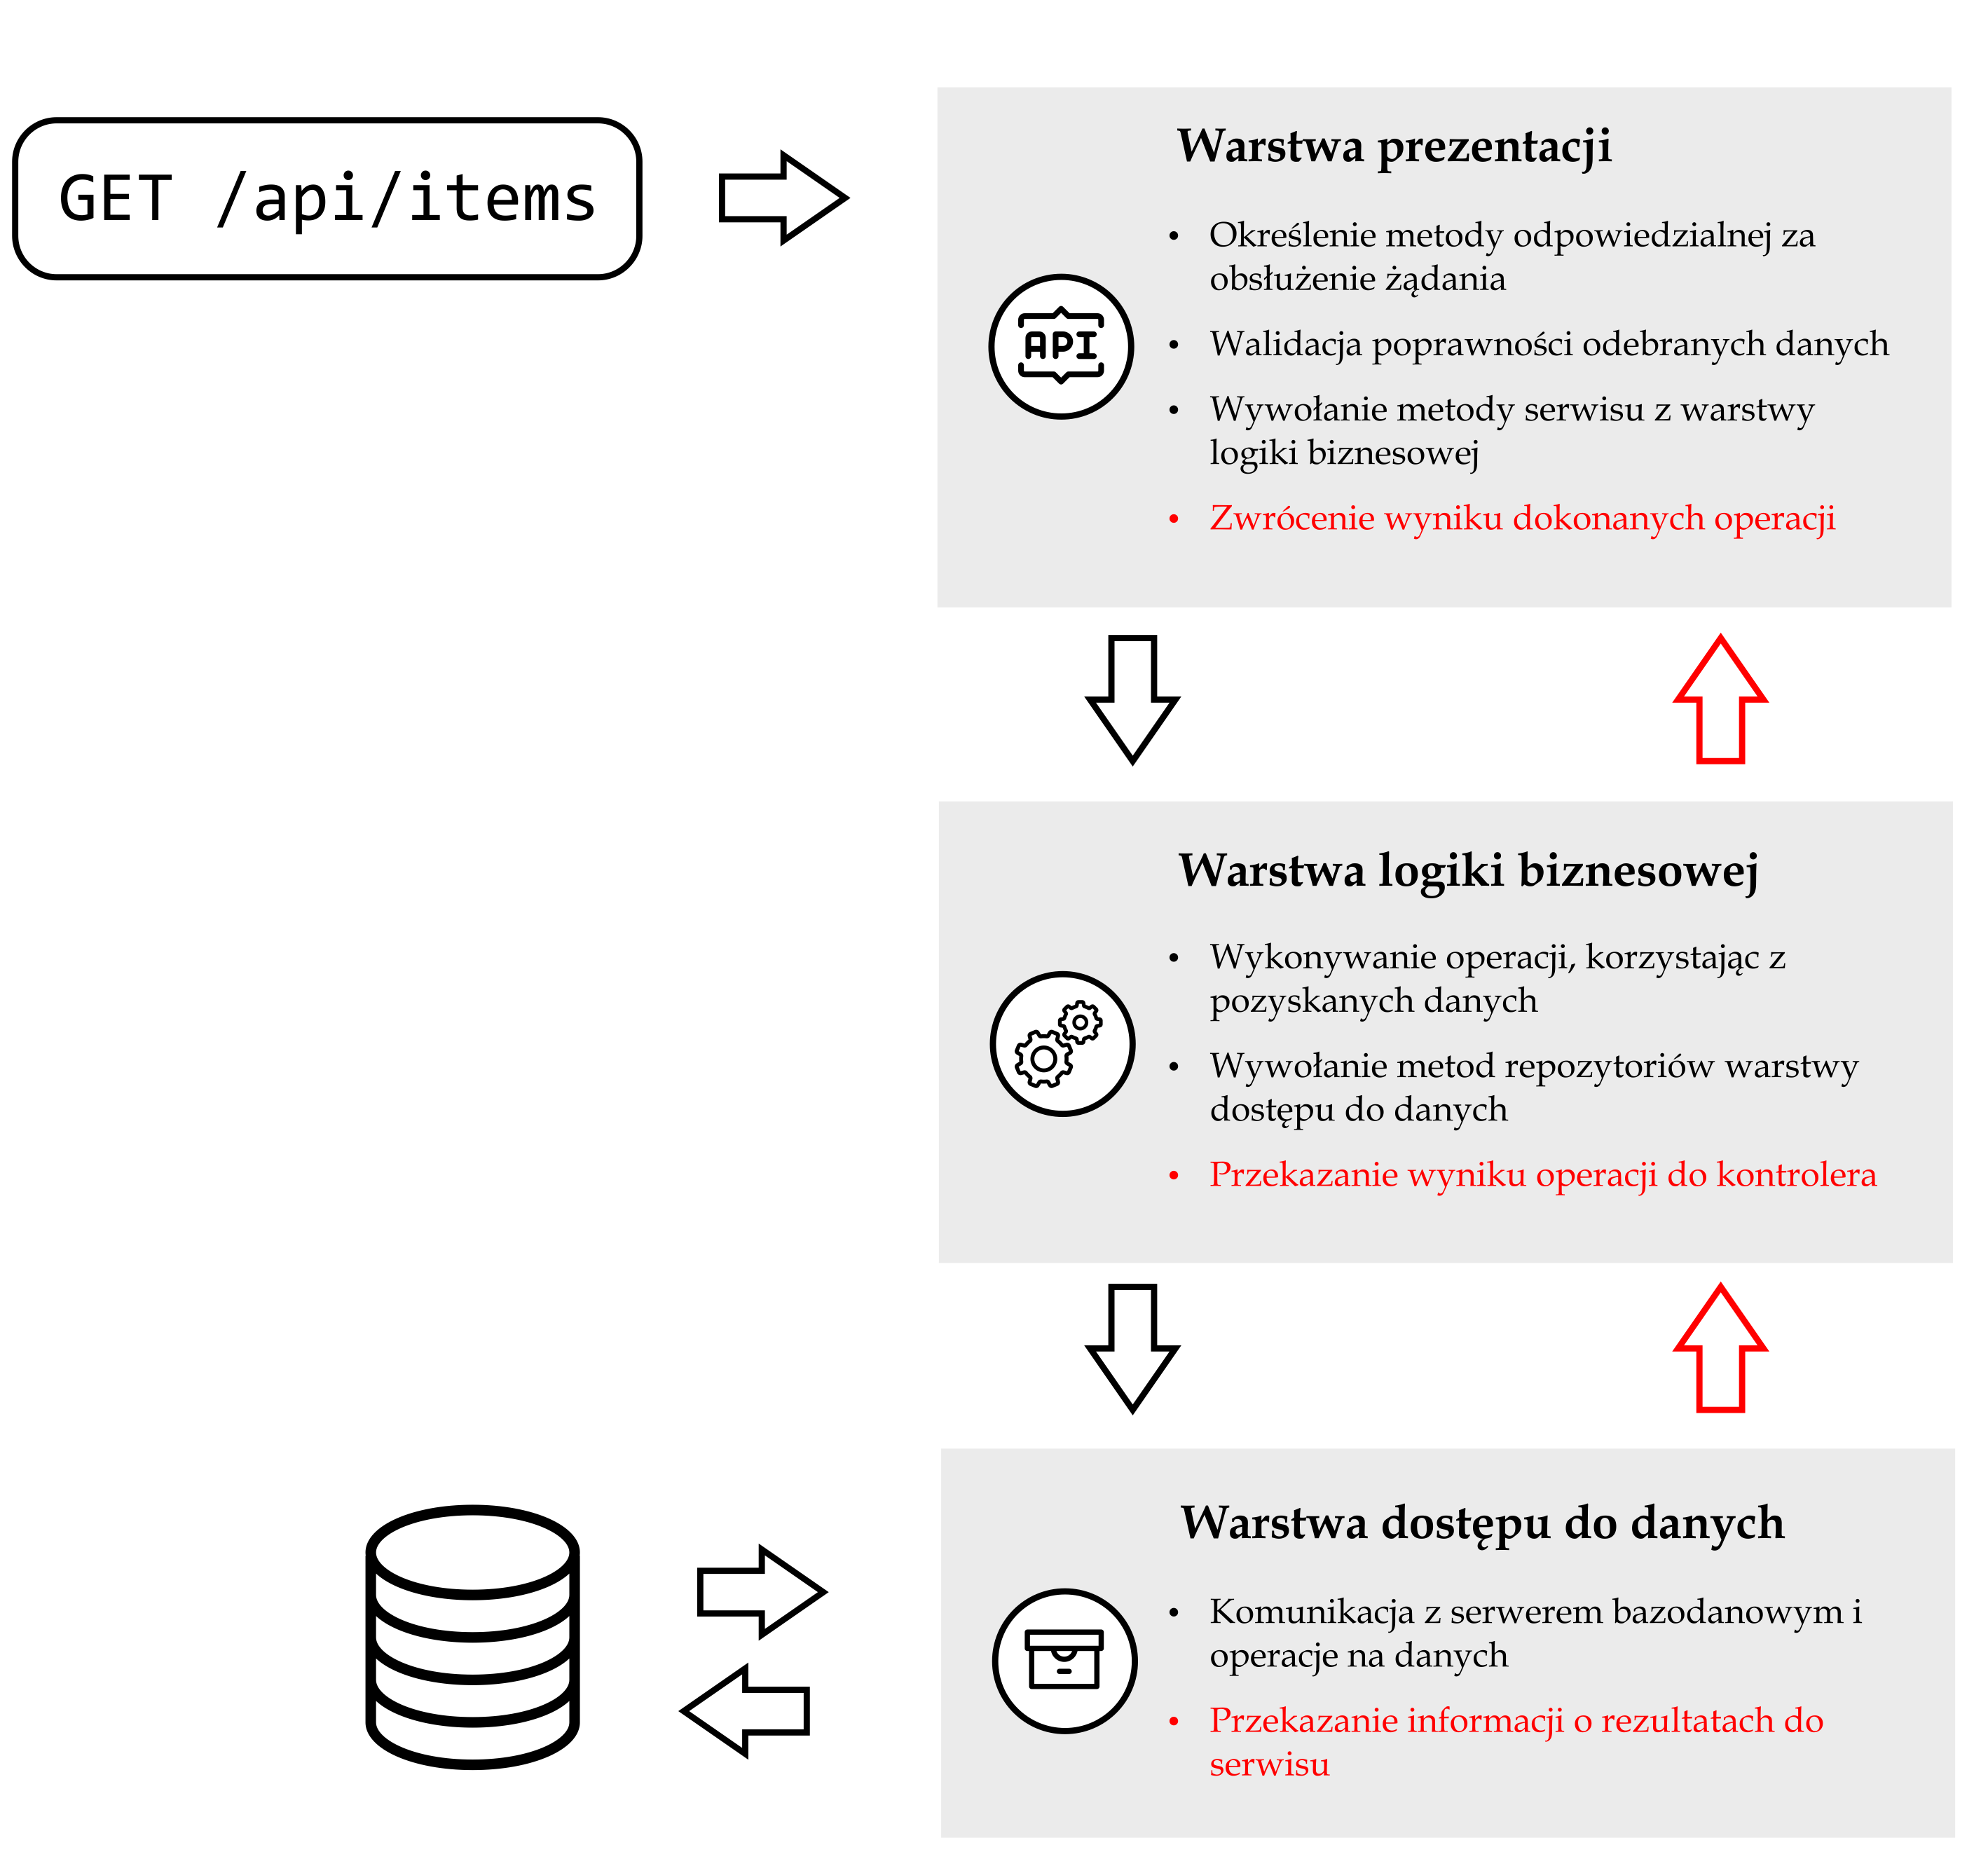
\includegraphics[width=0.9\linewidth]{rys02/architektura-api}
 \caption{Proces przetwarzania żądania wewnątrz interfejsu API}
 \label{fig:architektura-api}
\end{figure}
 
\subsection*{Konwersja obiektowo-relacyjna}
W celu uproszczenia procesu pozyskiwania oraz modyfikacji danych z zewnętrznych źródeł, a także unifikacji sposobu interakcji z nimi w ramach interfejsów programowania aplikacji powszechnie wykorzystywane jest oprogramowanie zwane mapperem obiektowo-relacyjnym (\textit{ang. Object-Relational Mapper}). Założeniem oprogramowania tego jest zdefiniowanie warstwy abstrakcji pomiędzy interfejsem programowania aplikacji a językiem programowania bądź zbiorem poleceń wykorzystywanym w ramach obsługi źródła danych.

Podstawowe składowe oprogramowania typu ORM to jednolity interfejs operacji na zbiorze danych, klasy kontekstu bazodanowego, a także metody obsługi komunikacji z bazą danych.

Dzięki wprowadzeniu jednolitego interfejsu operacji na danych niezależnie od źródła informacji z jakim komunikuje się API wydanie konkretnego polecenia do dowolnego systemu bazodanowego równoznaczne jest z każdorazowym wywołaniem funkcji o takiej samej sygnaturze. Stosując takie podejście, konstruktor interfejsu programowania aplikacji nie staje się uzależniony od źródła danych z którym pracuje. Ponadto, istnieje możliwość zamiany lub połączenia dodatkowego systemu bazodanowego, a operacja ta, nie wpływa w jakikolwiek sposób na działanie interfejsu API. Niniejsza zależność została zilustrowana na rysunku \ref{fig:orm-wyjasnienie}

\begin{figure}[ht]
 \centering
  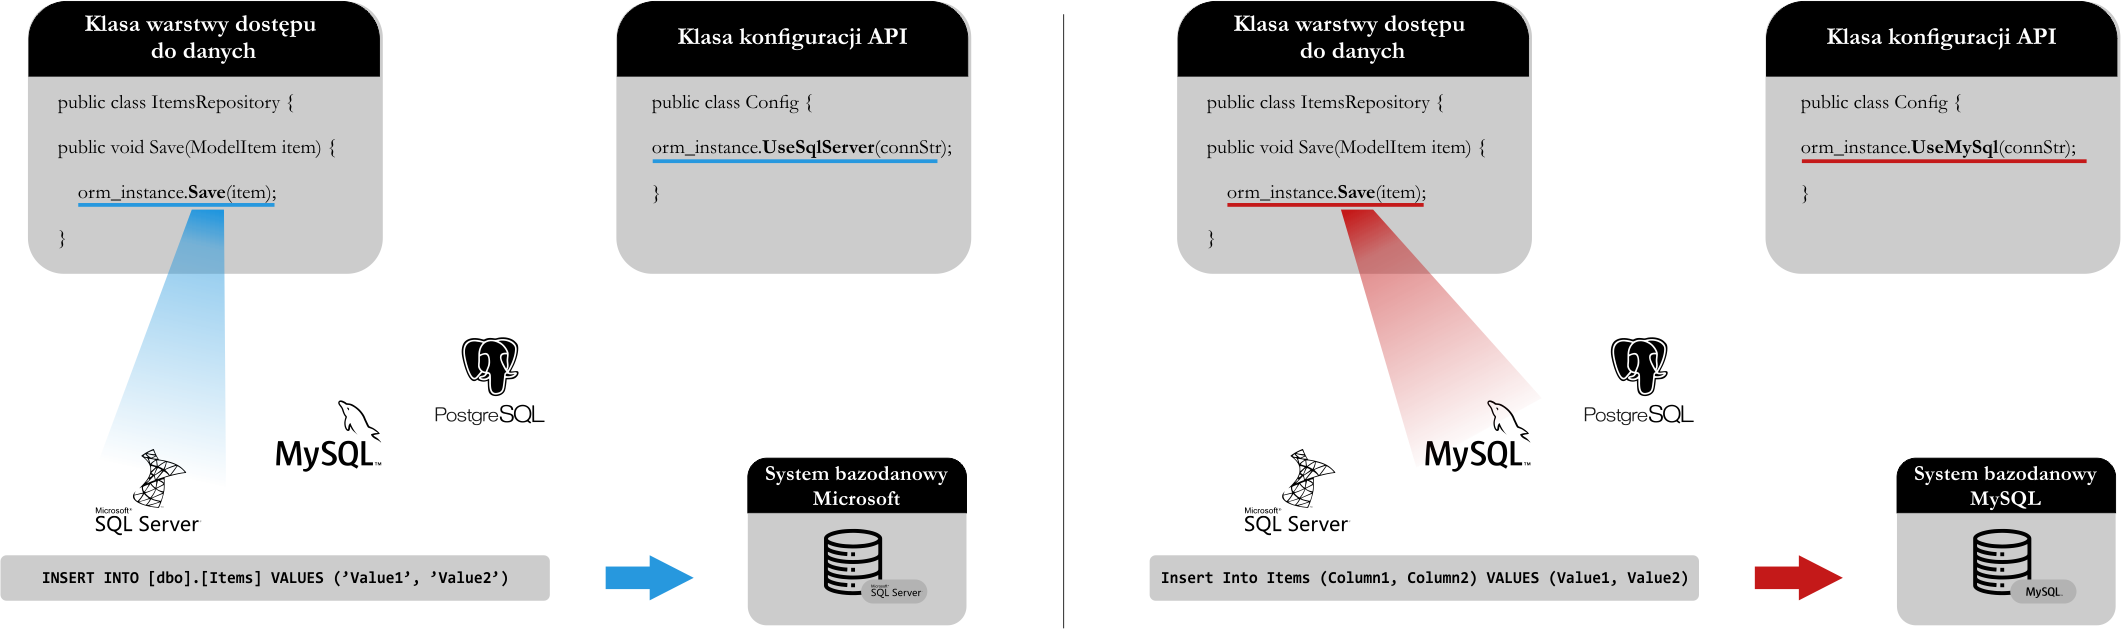
\includegraphics[width=1\linewidth]{rys02/orm-wyjasnienie}
 \caption{Zasada działania oprogramowania mappera obiektowo-relacyjnego w kontekście jednolitego interfejsu operacji na zbiorze danych}
 \label{fig:orm-wyjasnienie}
\end{figure}

Dystynktywnym elementem oprogramowania mappera obiektowo-relacyjnego jest klasa kontekstu bazodanowego. Klasa ta, jest kontenerem struktur w ramach których wyróżnić możemy zbiory elementów modelu danych, a także konfigurację poszczególnych ich właściwości. Podstawową ideą omawianej konwersji dziedziny obiektowej do domeny relacyjnej jest zdefiniowanie zbioru klas opisujących wykorzystywane zasoby, a następnie odwzorowanie ich w relacyjnym modelu danych obsługiwanym przez wybrany system bazodanowy. Klasa kontekstu pozwala na określenie, które spośród struktur danych zdefiniowanych w ramach API powinny zostać rzutowane na obiekty tabel generowanych w obrębie bazy danych. Ponadto, dla właściwości każdej z klas modelu danych zdefiniować należy konfigurację, która zostanie przetransformowana do modelu relacyjnego. W zakresie klasy kontekstu bazy danych opisywane są także relacje jakie mają zostać wygenerowane pomiędzy poszczególnymi elementami modelu.

W celu nawiązania, utrzymania, a także zakończenia komunikacji z zewnętrznym źródłem danych, oprogramowanie ORM wykorzystuje klasy zwane konektorami. Klasy te, dostarczają przejrzysty interfejs obsługi połączenia, który następnie jest opakowywany w zunifikowany interfejs dostępny bezpośrednio dla twórcy API \cite{TORRES20171}.

\subsection*{Uwierzytelnienie oraz autoryzacja}
Proces uwierzytelnienia oraz autoryzacji użytkownika odwołującego się do interfejsu programowania aplikacji przedstawić należy w trzech następujących krokach.

Pierwszym z nich jest wygenerowanie żądania odwołującego się do punktu końcowego odpowiedzialnego za obsługę uwierzytelnienia wewnątrz API. Żądanie to, musi posiadać ciało zawierające informacje poświadczające o konkretnymi użytkowniku. Najczęściej informacją tą jest nazwa użytkownika oraz hasło.

Następnie dostarczone referencje są analizowane przez mechanizmy uwierzytelniania implementowane w ramach API. W rezultacie tych operacji zwrócona zostaje pozytywna odpowiedź zawierająca token autoryzujący bądź też negatywna posiadająca w sobie informację o błędzie uwierzytelnienia klienta.

Strona kliencka może autoryzować dysponowane operacje przed interfejsem programowania aplikacji uwzględniając w ramach linii nagłówkowej żądania token uwierzytelniający. Dostarczona w ten sposób informacja pozwala na identyfikację użytkownika w ramach interfejsu API, a także na określenie przypisanego użytkownikowi poziomu uprawnień. W ramach struktury tokenu zawarta jest także informacja o jego czasie ważności. Dlatego też, procedura uwierzytelniania musi być regularnie ponawiana \cite{lakshmiraghavan2013pro}.

Na rysunku \ref{fig:uwierzytelnienie-autoryzacja} zilustrowany został proces uwierzytelnienia i autoryzacji aplikacji klienta przez interfejsem programowania aplikacji. 

\begin{figure}[ht]
 \centering
  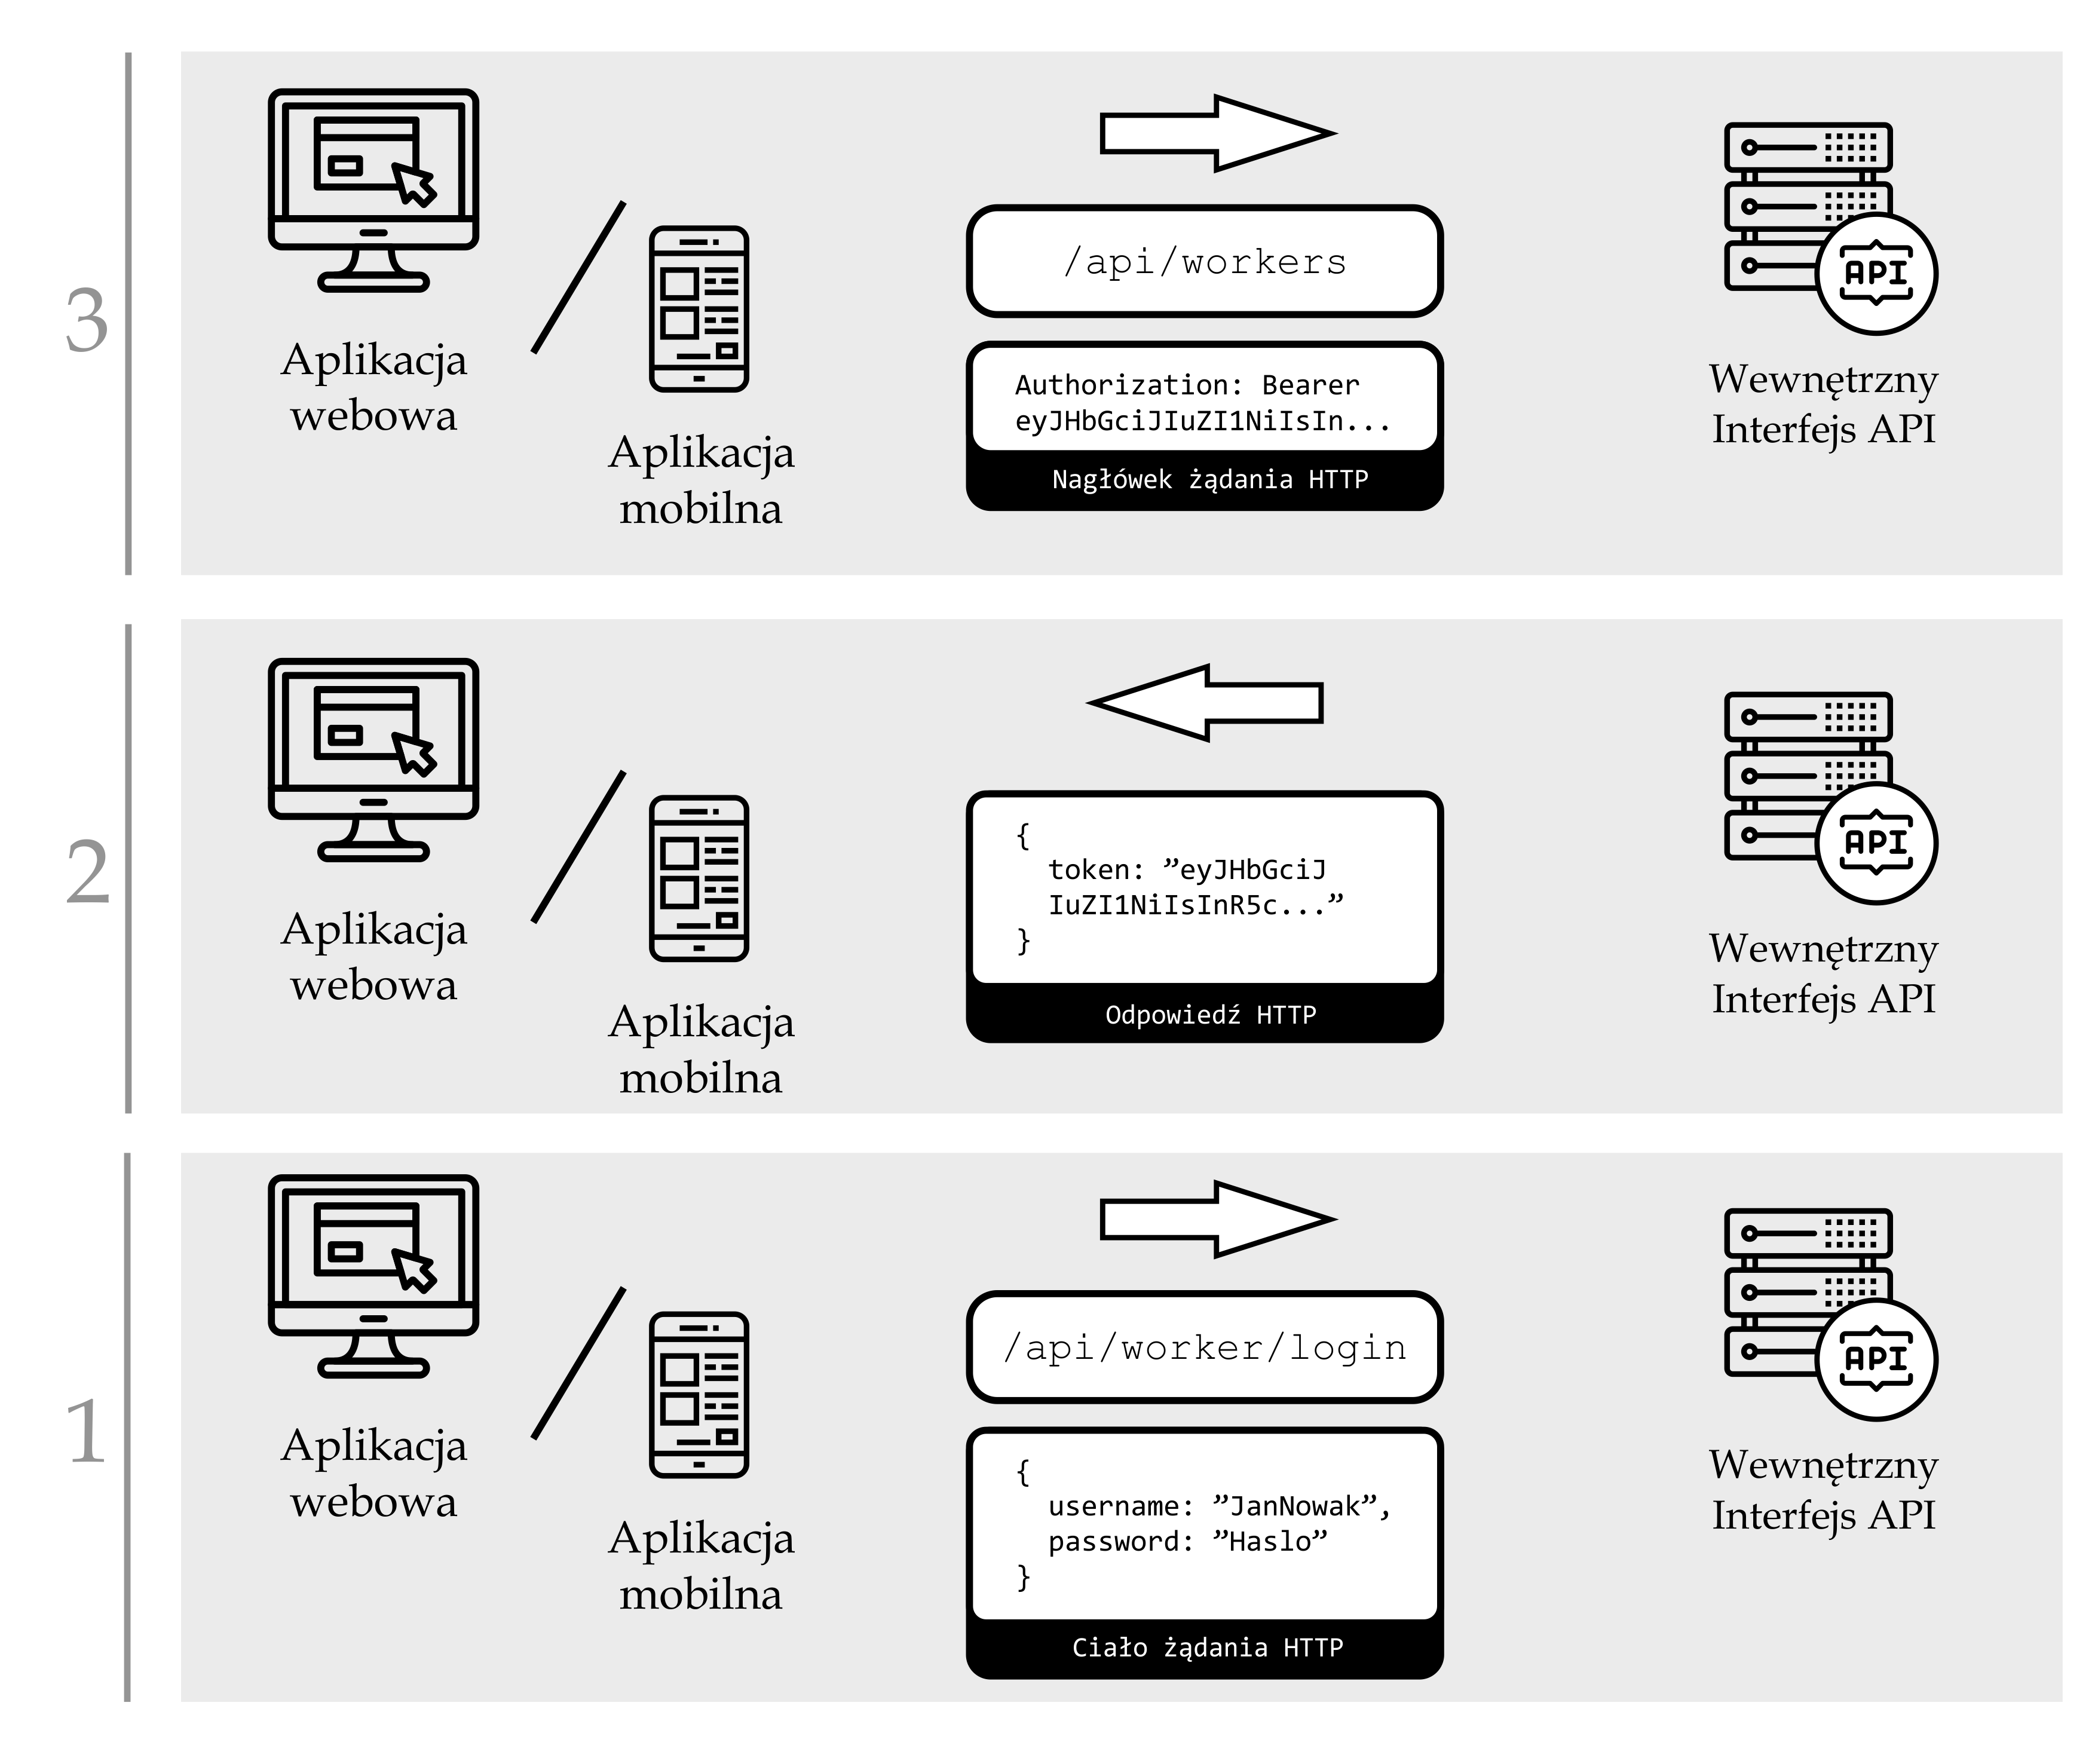
\includegraphics[width=1\linewidth]{rys02/uwierzytelnianie-autoryzacja}
 \caption{Proces uwierzytelnienia oraz autoryzacji użytkownika przed interfejsem API}
 \label{fig:uwierzytelnienie-autoryzacja}
\end{figure}


\subsection*{Separacja zapytań oraz komend w kontekście odwołań do źródeł danych}
Wraz z rosnącą liczbą żądań obsługiwanych w ramach zaawansowanych interfejsów programowania aplikacji zauważone zostało zjawisko asymetrii w kontekście typów wiadomości generowanych przez klientów. Zapytania dotyczące pozyskiwania danych z API realizowane jest z nieporównywalnie większą częstością niż operacje ich modyfikacji. Dlatego też, zdefiniowany został wzorzec projektowy dotyczący separacji zapytań oraz komend generowanych względem usługi sieciowej \textit{(ang. Command Query Responsibility Segregation)}.

Zastosowanie przedstawionego powyżej wzorca projektowego wiąże się z koniecznością budowy dwóch osobnych modeli danych. Pierwszy z nich, wykorzystywany jest w kontekście odczytu informacji. Na modelu tym, dokonywana jest najczęściej operacja optymalizacji, której celem jest redukcja rozmiaru składowych modelu, a także szybkości przetwarzania bardziej złożonych struktur będących jego częścią. Drugi z modeli danych znajduje zastosowanie w aspekcie modyfikacji określonych zasóbów. Biorąc pod uwagę standardowy sposób eksploatacji interfejsu programowania aplikacji model ten cechować się może niższą wydajnością. W zależności od specyfiki określonej usługi sieciowej optymalizowany może być albo model odczytu, albo też model zapisu. Ponadto, implementując wzorzec projektowy separacji zapytań oraz komend wykorzystać można dwa osobne zewnętrzne źródła danych przystosowane do wydajniejszego wykonywania określonego typu operacji bądź też dostosowane do obsługi większego ruchu sieciowego.   

Niewątpliwymi zaletami wynikającymi z zastosowania opisywanego wzorca projektowego są: zwiększenie efektywności operacji realizowanych z dużą częstotliwością, możliwość korzystania z osobnych źródeł danych dla operacji odczytu oraz zapisu, zachowanie zasady pojedynczej odpowiedzialności \textit{(ang. Single Responsibility Principle)} względem klas logiki biznesowej API, a także redukcja liczby wstrzykiwanych zależności \textit{(ang. Dependency Injection)} w ramach klas kontrolerów interfejsu \cite{cs7194}.

Na ilustracjach \ref{fig:standard-vs-cqrs1} oraz \ref{fig:standard-vs-cqrs2} przedstawiono kolejno schemat przetwarzania żądań wewnątrz API z uwzględnieniem wzorca CQRS, a także przy wykorzystaniu pojedynczego modelu danych.

\begin{figure}[ht]
    \centering
     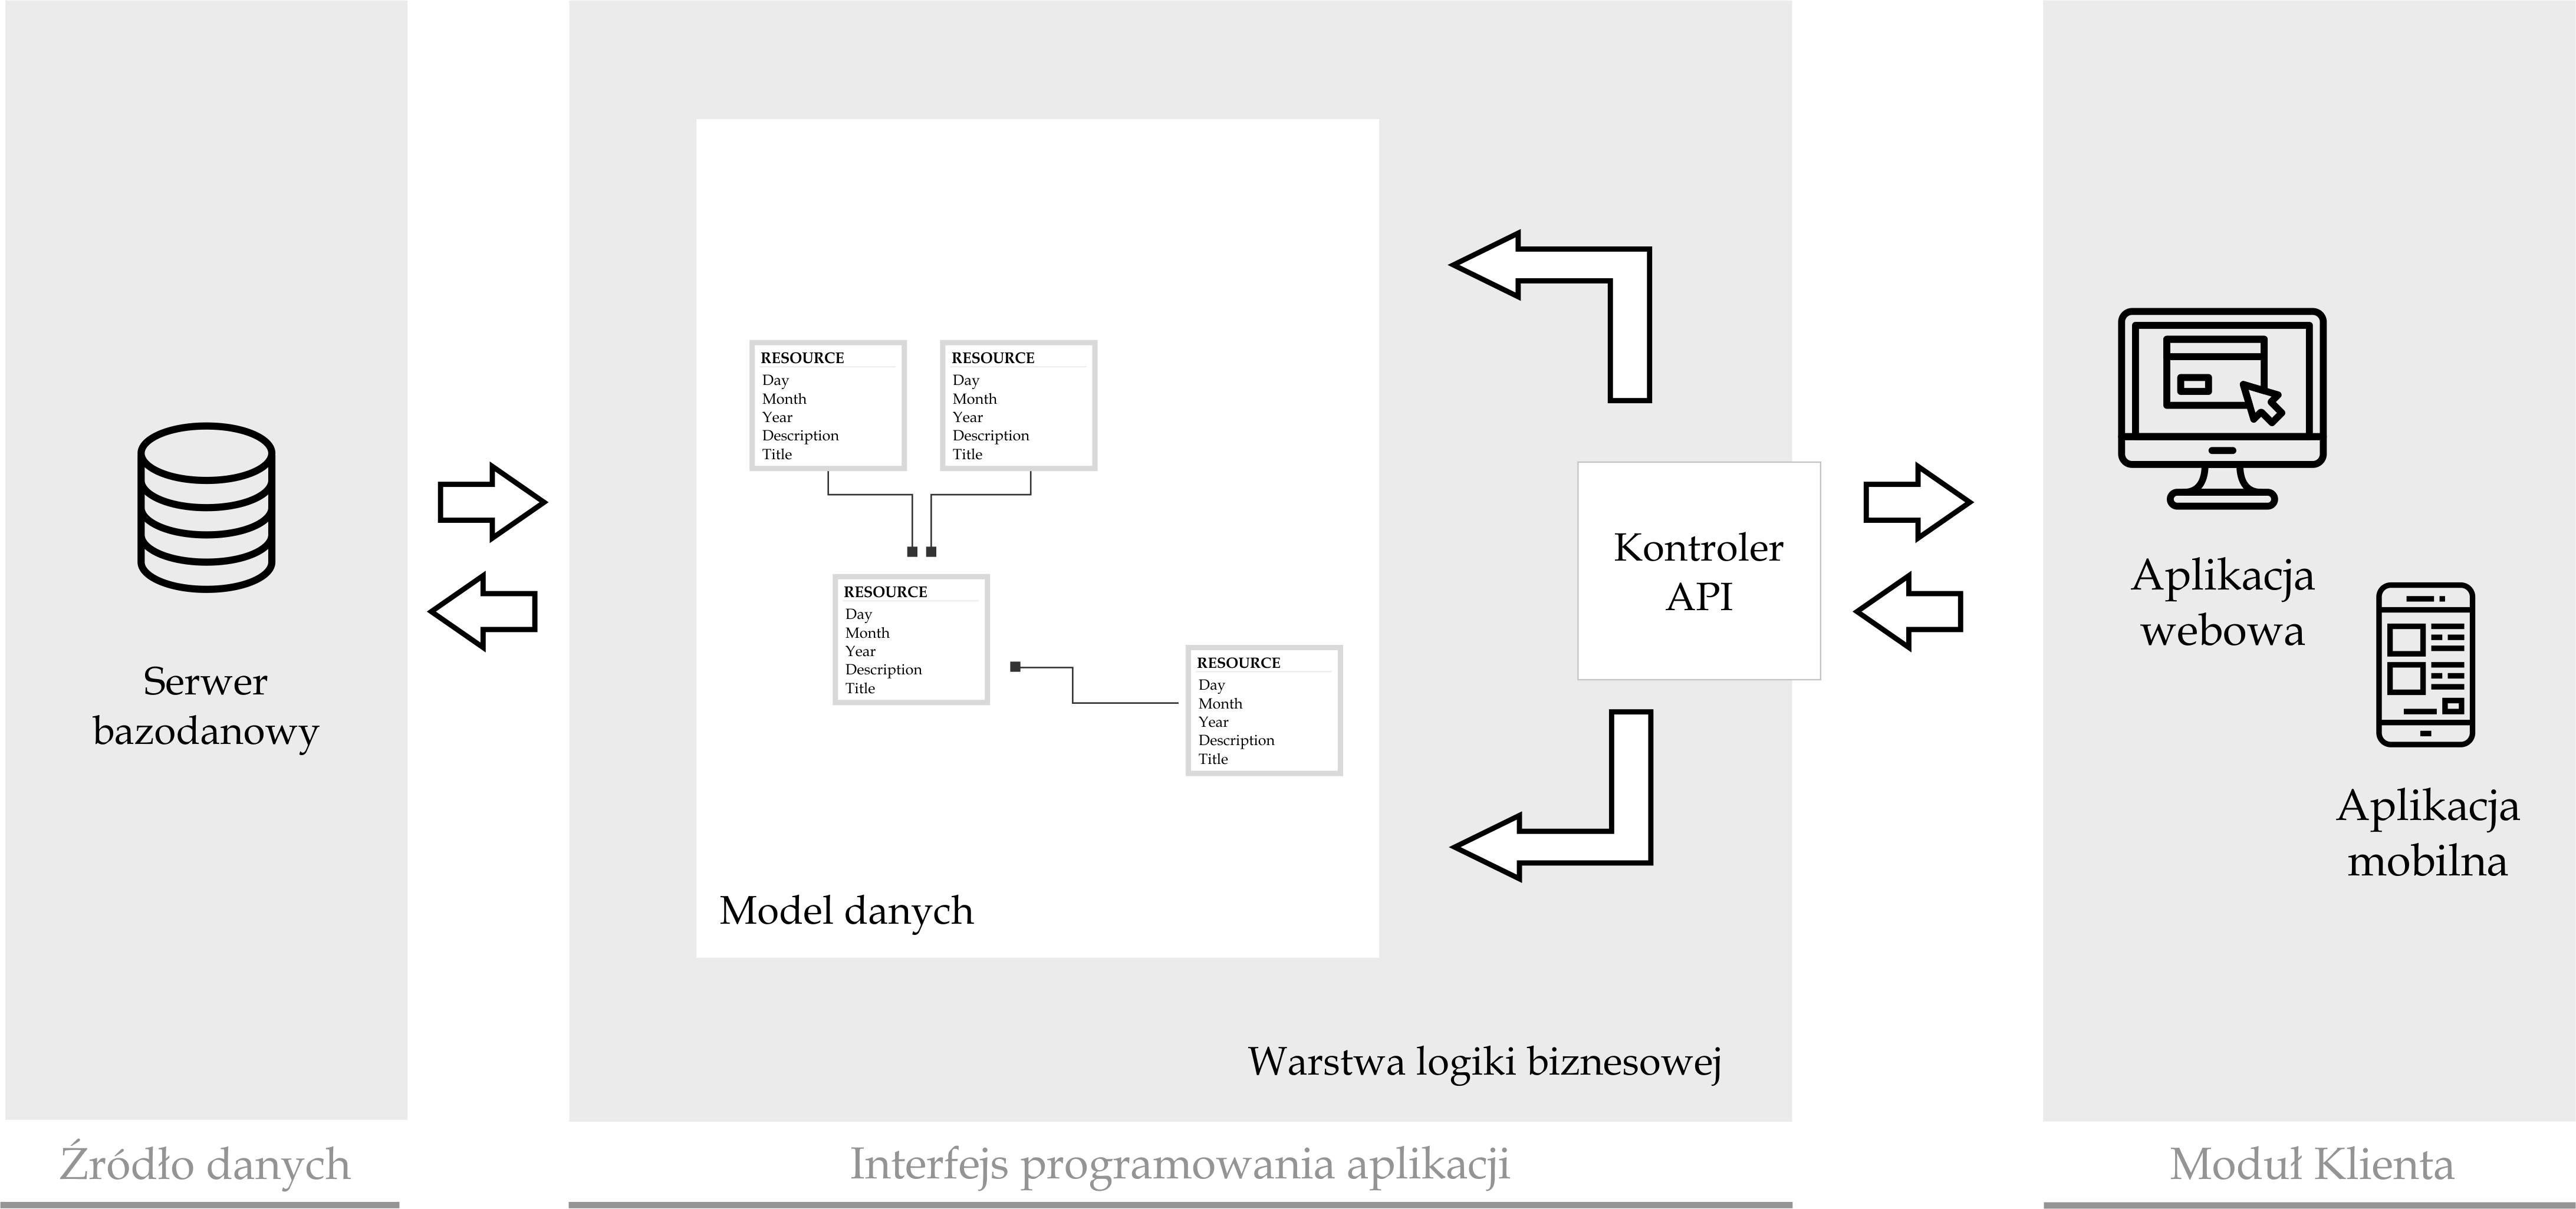
\includegraphics[width=0.9\linewidth]{rys02/standard-vs-cqrs1.png}
    \caption{Schemat przetworzenia żądania przez interfejs API dla architektury z jednym modelem danych}
    \label{fig:standard-vs-cqrs1}
   \end{figure}

   \begin{figure}[ht]
    \centering
     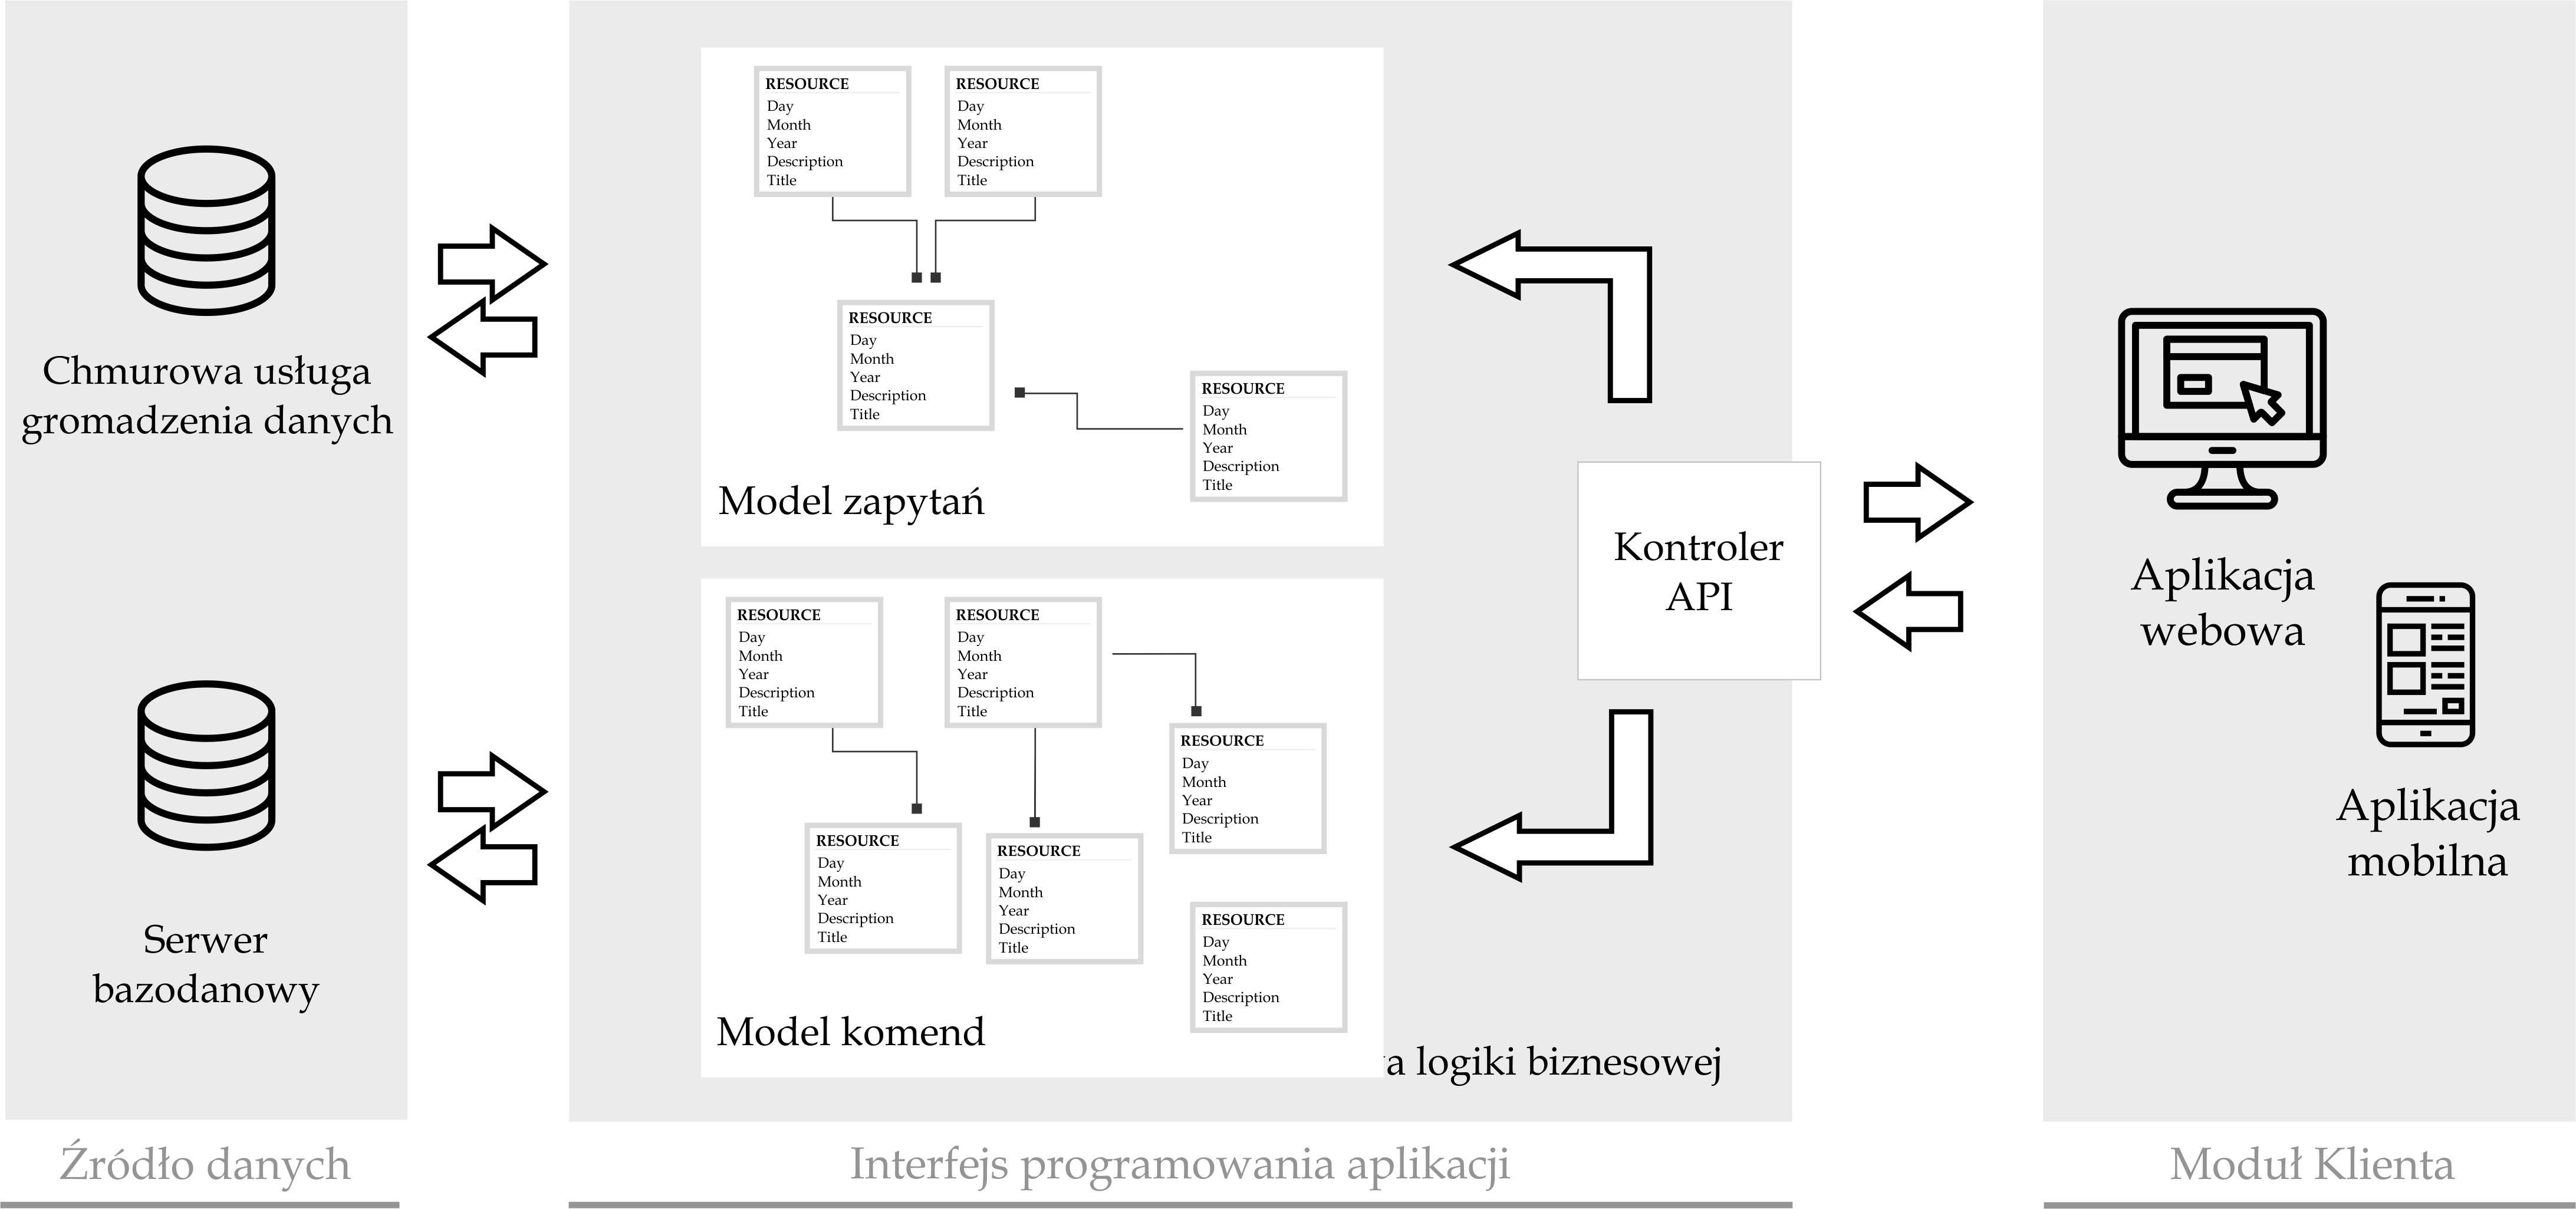
\includegraphics[width=0.9\linewidth]{rys02/standard-vs-cqrs2.png}
    \caption{Schemat przetworzenia żądania przez interfejs API dla architektury wykorzystującej wzorzec projektowy CQRS}
    \label{fig:standard-vs-cqrs2}
   \end{figure}


Odwołując się do ilustracji \ref{fig:standard-vs-cqrs2} należy zaznaczyć, że jest to jedna z możliwości implementacji wzorca CQRS uwzględniająca wykorzystanie odseparowanych źródeł danych. Architektura separacji zapytań oraz komend w kontekście żądań wysyłanych do interfejsu API może być także wprowadzona przy wykorzystaniu pojedynczego systemu bazodanowego.

\subsection*{Konwencja REST}
Niezależnie od struktury wewnętrznej omawianych usług sieciowych, współczesne interfejsy programowania aplikacji projektowane są tak aby ich zewnętrzna warstwa (tj. widziana z perspektywy aplikacji klienckiej) cechowała się jednolitą kompozycją.

Jednym z najpopularniejszych sposobów zapewnienia jednolitego interfejsu komunikacyjnego pomiędzy klientami i usługami sieciowymi przetwarzającymi informacje z wykorzystaniem protokołu HTTP jest konwencja oraz styl architektoniczny REST \textit{(ang. Representational State Transfer)}.

Konwencja ta, definiuje zbiór zasad dotyczących m.in. zachowania usługi sieciowej w kontekście przetwarzania żądania konkretnego typu, struktury i elementów odpowiedzi na określone żądanie, semantyki wykorzystywanych statusów rezultatu przetwarzania, bezstanowego charakteru komunikacji czy też syntaktyki odwołań do poszczególnych punktów końcowych.

W kontekście stopnia implementacji stylu architektonicznego REST w ramach interfejsu programowania aplikacji wprowadzić należy pojęcie modelu dojrzałości Richardsona \textit{(ang. Richardson Maturity Model)}. Pojęcie to definiuje cztery poziomy przystosowania interfejsu API do omawianej w niniejszej sekcji konwencji.

W odniesieniu do poziomu zerowego, powinnością interfejsu programowania aplikacji jest udostępnienie usług w ramach pojedynczego adresu sieciowego niezależnie od wykorzystywanych metod HTTP. Struktura żadania klienckiego w sposób jednoznaczny dostarczać ma informację na temat wykonywanego wewnątrz usługi sieciowej działania.

Zasada poziomu pierwszego odnosi się do charakterystyki interfejsu API jako usługi zorientowanej na zasoby. Niezależnie od czynności jaka ma zostać wykonana przez omawianą usługę sieciową opis tej czynności wskazywać ma na zasób którego ona dotyczy.

Reguła stanowiąca definicję poziomu trzeciego związana jest z semantyką poszczególnych typów żądań protokołu hipertekstowego. Żądanie o takim samym adresie sieciowym pełnić powinno odmienną rolę w zależności od rodzaju żądania HTTP.

Ostatnim z poziomów dojrzałości interfejsu programowania aplikacji opartego o konwencję REST jest reguła HATEOAS \textit{(ang. Hypertext As The Engine Of Application State)}. Reguła ta, definiuje interfejs API jako źródło informacji dotyczącej obsługi stanu całego systemu internetowego (tj. usługi sieciowej wraz z aplikacjami klienckimi). Klient, po uzyskaniu odpowiedzi serwera na żądanie powinien na podstawie zawartości tej odpowiedzi móc zdefiniować przyszłe czynności które wolno mu wykonać \cite{webber2010rest}.  

\section{Testowanie oprogramowania}
Aspekt badawczy niniejszej pracy związany jest z realizacją procesu ewaluacji wydajności interfejsów programowania aplikacji pod kątem wykorzystania odmiennych środowisk implementacyjnych oraz uruchomieniowych. Proces ten, jest tylko jednym z wielu elementów domeny testowania oprogramowania, której charakterystyka uwzględnia zbiór sztywno zdefiniowanych reguł cechujących się wysokim poziomem sformalizowania. W następnych sekcjach niniejszego akapitu dokonane zostało wprowadzenie dotyczące zagadnienia ewaluacji oprogramowania, nakreślone zostały zasady testowania systemów informatycznych, zdefiniono taksonomię technik testowania, a także omówiono proces przeprowadzania ewaluacji wydajności usługi sieciowej jaką jest interfejs programowania aplikacji. 
\subsection*{Wprowadzenie do zagadnienia ewaluacji oprogramowania}
Ewaluacja poszczególnych składowych tworzonego oprogramowania jest niezbędną częścią procesu budowy systemu informatycznego niezależnie od jego charakterystyki, czy też wykorzystywanej do jego budowy technologii. W rozumieniu ogólnym, proces testowania często sprowadzany jest do zbioru dwóch czynności. Czynnościami tymi są uruchamianie oprogramowania, a także eksploracja jego funkcjonalności w celu dostrzegania tych w ramach których zauważyć można niezgodność ich działania w stosunku do specyfikacji. Takie wnioskowanie jednak jest niepełne i uwzględnia ono tylko jeden z etapów składających się na cały proces testowania. Dziedzinę ewaluacji cech programów komputerowych poszerzyć należy ponadto o takie elementy jak: planowanie testów, wybór kryteriów oceny oprogramowania, nadzór oraz kontrolę realizacji badań, projektowanie przypadków testowych, czy też analizę spełnienia ustalonych kryteriów zakończenia.

Wyróżnić możemy znaczącą liczbę definicji testowania oprogramowania a każda z nich wprowadza inny poziom szczegółowości. Ponadto, wiele spośród formułowanych pojęć nawiązuje do różnych aspektów omawianego procesu. Zgodnie z jedną z najbardziej generycznych definicji wprowadzoną przez Hetzla w publikacji \cite{hetzel}, proces testowania oprogramowania określić należy jako zbiór wszystkich czynności, które nakierowane są na weryfikację atrybutów i właściwości programu, a także sprawdzenie tego czy określony system spełnia założone wymagania. Definicja ta względem wielu innych popularnych sformułowań dotyczących ewaluacji oprogramowania uwzględnia możliwość zastosowania statycznych technik testowania. Ponadto, jej autor bierze pod uwagę fakt, że w ramach procesu ewaluacji oceniany powinien być każdy z artefaktów tworzonych w ramach systemu a nie tylko i wyłącznie kod źródłowy programu.
\subsection*{Taksonomia technik testowania}
Jako jedno z podstawowych kryteriów podziału technik testowania oprogramowania wskazać należy rodzaj czynności wykonywanej przez stronę testującą, której realizacja prowadzi do uzyskania charakterystyki programu poddanego ewaluacji. Według kryterium tego wyróżnić należy statyczne oraz dynamiczne techniki testowania.

Pierwsze spośród przytoczonych metod opierają się na analizie artefaktów oprogramowania (takich jak m.in.: kod źródłowy, specyfikacja, dokumentacja, czy też lista wymagań) bez ich wykonywania. Jako praktyczne przykłady przedstawionej techniki zdefiniować należy: generowanie metryk kodu źródłowego programu, analizę przepływu sterowania, formalne dowodzenie poprawności działania, a także interpretację grafów wywołań.

Metody dynamiczne natomiast związane są z weryfikacją właściwości poszczególnych elementów systemu informatycznego w trakcie jego wykonywania. Ten rodzaj testowania nie uwzględnia formalnych struktur liczbowych jakimi są grafy przepływu sterowania czy też metryki kodu źródłowego programu. Zorientowany jest on na odbiór systemu z perspektywy korzystającego z niego klienta.

Innym z rozważanych kryteriów podziału technik testowania jest ich umiejscowienie metody względem określonego fragmentu procesu wytwórczego. W nawiązaniu do tego aspektu zdefiniować należy pojęcie poziomu testów, które jest powiązaniem sposobu ewaluacji oprogramowania z etapem jego realizacji. Istotą rozróżniania danych poziomów testów jest założenie różnorodności celów testowania, a także testowanych obiektów określanych w kontekście każdej z warstw. W odniesieniu do najbardziej popularnych systematyk poziomów testowania wyróżnić można następujące elementy:
\begin{itemize}
    \item testy jednostkowe (zwane także modułowymi lub testami komponentów),
    \item testy integracyjne,
    \item testy systemowe,
    \item testy akceptacyjne.
\end{itemize}

Pierwszy z poziomów dotyczy znajdowania niezgodności specyfikacyjnych w obrębie logicznie oddzielonych jednostek oprogramowania \textit{(ang. Software Units)}. Każda z jednostek powinna być testowana w izolacji od pozostałych elementów systemu. Ze względu na złożoność rozwiązań informatycznych, a także statystycznie wysoki współczynnik wzajemnych zależności modułowych warunek ten często nie może zostać spełniony. W takich sytuacjach, aby dostarczyć zależność do testowanej jednostki budowane są moduły zastępcze imitujące poprawne zachowanie określonego fragmentu programu \textit{(ang. Mocks)}. Omawiany poziom testowania często postrzegany jest jako jeden z etapów procesu wytwórczego, szczególnie w ramach takich technik jak rozwój oprogramowania napędzany testowaniem \textit{(ang. Test Driven Development)}.

Celem kolejnego z poziomów testowania jest weryfikacja poprawności współoddziaływania indywidualnych komponentów a także prawidłowości funkcjonowania interfejsów definiowanych pomiędzy nimi. Przykładem współdziałania jednostek oprogramowania może być współpraca interfejsu programowania aplikacji będącego systemem poddawanym analizie w ramach niniejszej pracy, a także określonego silnika bazodanowego. W zależności od liczności weryfikowanych powiązań pomiędzy poszczególnymi jednostkami oprogramowania, a także w odniesieniu do liczby samych modułów będących częścią testowanego fragmentu systemu wyróżnić możemy testy małej oraz dużej skali integracji.

Na temat testów systemowych należy mówić wtedy, gdy wszystkie z elementów rozwiązania informatycznego zostały ze sobą powiązane w sposób spójny. Celem testów realizowanych w ramach tego poziomu jest weryfikacja wysokopoziomowej funkcjonalności oprogramowania, a także wykonywanie scenariuszy ewaluacji systemu z poziomu regularnego użytkownika \textit{(ang. End-to-End testing)}.

Ostatnim z wymienionych poziomów ewaluacji są testy akceptacyjne. Przedmiotem oceny w ramach tego rodzaju testów jest gotowe rozwiązanie informatyczne w postaci komercyjnego produktu. Podmiot odpowiedzialny za realizację omawianych testów przygotowuje listę kryteriów akceptacji \textit{(ang. acceptance criteria)} a następnie na podstawie obsługi testowanego rozwiązania potwierdza lub odrzuca spełnienie każdego z nich. Celem omawianych ewaluacji nie jest znajdowanie błędów działania systemu a nabranie zaufania co do jakości jego funkcjonalnych oraz niefunkcjonalnych atrybutów.

Wykonując testy definiowane w ramach kolejnych poziomów ewaluacji weryfikowane zostają na początek funkcjonalne, a następnie niefunkcjonalne elementy testowanego systemu. Jako weryfikację elementów funkcjonalnych rozumieć należy wszystkie te czynności, które podejmowane są w ramach wszystkich wymienionych powyżej poziomów testów z wyjątkiem testów akceptacyjnych. Ewaluacja niefunkcjonalna natomiast odnosi się tylko do ostatniego spośród wyróżnionych poziomów testowania.

Podział charakteryzujący przedmiot ewaluacji względem omówionych aspektów definiuje pojęcia testów funkcjonalnych oraz niefunkcjonalnych i w kontekście niniejszej pracy jest on podziałem kluczowym.

Badania przeprowadzone w ramach tej pracy posiadają charakter testów niefunkcjonalnych, a ich wykonanie poprzedzone jest weryfikacją funkcjonalną, której poprawność traktowana jest jako wymóg.
\subsection*{Ewaluacja wydajności interfejsów programowania aplikacji}
Zgodnie z teorią przedstawioną w sekcji \ref{sec:api-teoria} niniejszej pracy interfejs programowania aplikacji postrzegać można jako deterministyczny system wejściowo-wyjściowy o charakterze dyskretnym. Takie podejście, w znaczący sposób ułatwia proces ewaluacji wydajności interfejsów API.

Definiowanie interfejsu API jako systemu pobudzanego pojedynczym wejściem, a także generującego pojedynczą wartość wyjściową, pozwala na wykorzystanie sposobu oceny wydajności zwanego testem czarnoskrzynkowym \textit{(ang. Black-box testing)}. W ramach tego rodzaju testu, określone kryterium ewaluacji wyliczane jest jako różnica wartości pomiaru na wyjściu systemu, względem tej, której kalkulacja nastąpiła na jego wejściu. Taki rodzaj testu, umożliwia wyliczenie metryki wydajności, bez konieczności przygotowywania systemu do przeprowadzenia procesu testowania.

Podstawowym kryterium oceny wydajności interfejsu programowania aplikacji jest czas odpowiedzi na żądanie. Metrykę tę, określić należy jako czas od momentu wygenerowania żądania przez stronę klienta, do chwili uzyskania przez niego odpowiedzi. Zauważyć należy również zależność czasu odpowiedzi na żądanie, zarówno od rozmiaru żądania jak i wielkości jego odpowiedzi. Ponadto, czynnikiem wpływającym na uzyskany rezultat pomiaru jest niewątpliwie przepustowość łącza sieciowego pomiędzy klientem a serwerem.

Aby rezultaty uzyskane w ramach oceny wydajności API mogły zostać postrzegane jako rzetelne, omówione powyżej czynniki muszą cechować się statyczną charakterystyką, bądź też zostać całkowicie wyeliminowane z procesu testowego. W ramach niniejszej pracy, rozmiar odpowiedzi generowanej przez interfejsy programowania aplikacji jest stały niezależnie od zastosowanej technologii, a także środowiska uruchomieniowego. Wynika to z zastosowania pojedynczego i ustrukturyzowanego modelu danych, który jest identyczny, niezależnie od API. W odniesieniu do zmienności prędkości łącza internetowego, aspekt ten został wyeliminowany poprzez przeprowadzanie testów w obrębie lokalnej sieci komputerowej, a także umiejscowienie interfejsów oraz systemów bazodanowych w ramach tej właśnie sieci.

Kolejnym z kryteriów oceny wydajności, uwzględnianym w ramach procesu testowania usług sieciowych jest poprawność uzyskanej odpowiedzi w odniesieniu do liczby klientów, równolegle generujących żądania. Kryterium to, charakteryzuje się silną korelacją z czasem odpowiedzi na pojedyncze zapytanie.

Uwzględniając oba opisane powyżej parametry, podstawowy schemat scenariusza badawczego dotyczącego ewaluacji wydajności API składa się z następujących testów:
\begin{itemize}
    \item testy linii bazowej -- pojedynczy klient generuje żadania w kierunku API w celu zdefiniowania średniego czasu odpowiedzi usługi w standardowych warunkach jej działania. W ramach niniejszej pracy, podczas wykonywania omawianego testu, zdefiniowane zostaną ponadto wartości współczynników satysfakcji, toleracji oraz frustracji, będące składowymi wskaźnika jakości APDEX. Wartości te, stanowią uogólnioną ocenę wydajności i posłużą jako punkt odniesienia dla kolejnych testów.
    \item testy obciążeniowe -- uwzględniana zostaje zmienna liczba klientów generujących żądania, w kontekście której ustalane są średnie czasu odpowiedzi na żądanie, a także dokonywane zostaje odniesienie uzyskanego rezultatu do współczynników zdefiniowanych uprzednio w ramach miary APDEX.
    \item testy przeciążające -- liczba klientów generujących żądanie zostaje dobrana w taki sposób, aby doprowadzić do obciążenia testowanej usługi, niepozwalającego na poprawne funkcjonowanie interfejsu programowania aplikacji. Ewaluacja ta, ma na celu znalezienie punktu krytycznego w kontekście działania testowanego oprogramowania.
\end{itemize}

Poza czarnoskrzynkowymi testami wydajności, cechującymi się omówioną powyżej strkturą, przeprowadzone mogą zostać ewaluacje efektywności działania poszczególnych fragmentów usługi sieciowej, w ramach których interfejs programowania aplikacji postrzegać należy w odmienny sposób, aniżeli jako system wejściowo-wyjściowy.

Przykładem oceny wydajności określonego fragmentu interfejsu programowania aplikacji może być ewaluacja modułu realizacji zaawansowanych operacji obliczeniowych, dostępnego z poziomu punktu końcowego API. W takim przypadku, oprogramowanie musi zostać dostosowane do przeprowadzenia procedury testowej, a metryka wydajności - powiązana z postępem realizacji obliczeń.
\section{Wykorzystywane narzędzia i technologie}
Zarówno w trakcie procesu implementacji badanych interfejsów programowania aplikacji, jak i procedurze przeprowadzenia badań pod kontem ich wydajności, wykorzystano obszerny zbiór sprawdzonych i powszechnie stosowanych rozwiązań technologicznych. W ramach niniejszej sekcji, opisane zostanie każde z nich.

\subsection*{C\#}
C\# jest wieloparadygmatowym, a także nowoczesnym językiem programowania ogólnego przeznaczenia, charakteryzującym się bezpieczeństwem i niezawodnością w aspekcie typowania struktur danych. Pierwsza z wersji tego języka, stworzona została przez Andersa Hejlsberga w roku 1998. Od tamtej chwili, do momentu napisania niniejszej pracy, upublicznionych zostało 9 kolejnych,  stabilnych wydań projektu C\#. Każda z następnych wersji omawianego języka programowania wprowadzała zarówno usprawnienia w kontekście ekosystemu budowy i kompilacji programów źródłowych, jak i wzbogacała interfejs bibliotek funkcyjnych o kluczowe z punktu widzenia doświadczonego programisty rozwiązania. Do rozwiązań tych, zaliczyć należy między innymi: mechanizmy programowania współbieżnego, typy anonimowe, operatory zmiennych typów niezdefiniowanych, obsługę referencji, typy generyczne, czy też wyrażenia lambda. 

W ramach niniejszej pracy, język C\# wykorzystany został do implementacji jednego z dwóch zbiorów interfejsów programowania aplikacji. Ze względu na zastosowanie rozwiązań z zakresu przetwarzania współbieżnego (tj. operacji asynchronicznych oraz wielowątkowych) udostępnianych przez omawiany język programowania, interfejsy API realizowane w tej technologii mogą obsługiwać w sposób równoległy żądania pochodzące od wielu klientów, a także utrzymywać sekwencyjny charakter przetwarzanych procedur niezależnie od czasu ich wykonywania. Należy także zwrócić uwagę na mechanizm wewnętrznych usprawnień wydajnościowych implementowany w ramach kompilatora i uruchamiany w momencie tłumaczenia kodu języka do tzw. języka pośredniego \textit{(ang. Intermediate Language)}. Dzięki zastosowaniu przedstawionego mechanizmu, operacje zdefiniowane przez programistę mogą być modyfikowane w procesie kompilacji, tak aby nie wpłynąć na zaimplementowaną funkcjonalność, zwiększając jednocześnie wydajność generowanego programu \cite{hejlsberg2003c}.
\subsection*{.NET Core}
.NET Core postrzegać należy jako środowisko budowy, kompilacji oraz wykonywania rozwiązań implementowanych w języku C\#. Przedstawiana technologia stanowi podzbiór bibliotek, dzięki którym programista jest w stanie budować systemy różnorodnego przeznaczenia, a także uruchamiać je w wielu wspieranych środowiskach programowych. W przeciwieństwie do technologii .NET Framework będącej poprzednikiem .NET Core, aplikacje tworzone na bazie omawianej biblioteki mogą być wydawane nie tylko na system operacyjny Windows, ale także na systemy Linux oraz MacOS.

W ramach omawianego środowiska wykorzystywany zostaje komponent języka C\# zwany biblioteką standardową \textit{(ang. .NET Standard Library)}. Biblioteka ta jest wspólna dla wielu środowisk uruchomieniowych, a zawarte w niej funkcjonalności, traktować należy jako metody ogólnego przeznaczenia.

Ponadto, środowisko .NET Core, w ramach procesu budowy i kompilacji rozwiązania nawiązuje komunikację z komponentem wspólnej infrastruktury \textit{(ang. Common Infrastructure)}. Komponent ten, podobnie jak biblioteka standardowa, współdzielony jest przez wiele środowisk wykonawczych. W kontekście wspólnej infrastruktury, wspomnieć należy o wspólnej specyfikacji języka \textit{(ang. CLS -- Common Language Specification)}, wspólnym systemie typów \textit{(ang. CTS -- Common Type System)}, a także środowisku uruchomieniowym wspólnego języka \textit{(ang. CLR -- Common Language Runtime)}. Wykorzystanie między innymi tych trzech elementów, pozwala na budowę systemu dostępnego na wielu platformach \cite{troelsen2017pro}.

W kontekście realizowanej pracy, technologia .NET Core użyta została jako środowisko uruchomieniowe dla interfejsów programowania aplikacji tworzonych w języku C\#. W obrębie technologii tej, poza przedstawionymi powyżej komponentami, wyróżnić możemy natywną bibliotekę ASP.NET Core, stanowiącą zbiór metod przydatnych w procesie definiowania internetowych usług sieciowych oraz aplikacji webowych. Dzięki zastosowaniu ASP.NET Core operacje takie jak, między innymi: obsługa definicji kontrolerów API, zarządzanie stanem ciała żądania oraz jego rzutowaniem na określony typ danych, czy też implementacja mechanizmów uwierzytelniania i autoryzacji klienta, wykonane mogą zostać na wysokim poziomie abstrakcji z jednoczesnym zapewnieniem należytego poziomu ich wydajności.
\subsection*{Entity Framework Core}
Entity Framework Core stanowi narzędzie stworzone przez firmę Microsoft, którego zastosowaniem jest mapowanie obiektowo-relacyjne realizowane w kontekście usług internetowych tworzonych z wykorzystaniem języka C\# oraz uruchamianych na platformie .NET Core. Przedstawiana biblioteka zapewnia programiście zorientowany obiektowo interfejs, za pomocą którego może on uzyskać dostęp do danych, a także je definiować oraz przetwarzać. Zbiory obiektów mogą być składowane zarówno w relacyjnych jak i niereleacyjnych bazach danych. Niniejsza biblioteka, podobnie do środowiska uruchomieniowego .NET Core, jest rozwiązaniem wieloplatformowym i może być wykorzystywana przy budowie systemów internetowych wdrażanych na systemach Windows, Linux oraz MacOS.

Zastosowanie biblioteki mapera obiektowo-relacyjnego jaką jest Entity Framework Core umożliwia zastosowanie podejścia zorientowanego na kod źródłowy w kontekście aplikacji komunikujących się i wykorzystujących zewnętrzne zbiory danych \textit{(ang. Code-First Approach)}. Podejście to, polega na definiowaniu w ramach kodu źródłowego zbioru klas modelu danych, które będą następnie przekształcane do postaci tabel określonego systemu bazodanowego. Przedstawiona operacja przekształcenia wykonywana jest bezpośrednio za pomocą mechanizmów mapera obiektowo-relacyjnego. 

Niezaprzeczalną zaletę wykorzystania biblioteki ORM jaką jest Entity Framework Core stanowi możliwość operowania na jednolitym interfejsie realizacji operacji na danych, niezależnie od obsługiwanego systemu bazodanowego. Oznacza to, że w momencie zmiany dostawcy zewnętrznego źródła danych, zawartość kodu źródłowego programu nie musi podlegać modyfikacji \cite{smith2021entity}.
\subsection*{MediatR}
MediatR to otwartoźródłowa biblioteka języka C\#, z wykorzystaniem której zaimplementowany może zostać wzorzec projektowy, dotyczący separacji odpowiedzialności za obsługę zapytań oraz komend przetwarzanych przez usługę sieciową. Kluczowym elementem biblioteki MediatR jest para generycznych interfejsów, za pomocą których implementowana jest obsługa zarówno żądań jak i zapytań dotyczących danych. Interfejsami tymi są kolejno: \textit{IRequest} -- struktura programistyczna implementowana przez klasy definiujące zawartość ciała żądania lub komendy, a także powiązany z nią \textit{IRequestHandler}, który jest konkretyzowany przez klasę definicji metody obsługi żądania bądź operacji na danych. 

Ponadto, należy również podkreślić znaczenie metody \textit{Send} dostępnej w ramach głównego API pakietu MediatR. Dzięki niej, wywołana może zostać procedura obsługi określonego żądania lub operacji, z dowolnego miejsca kodu źródłowego interfejsu programowania aplikacji \cite{mediatr}.
\subsection*{JavaScript}
JavaScript to wielofunkcyjny oraz wieloplatformowy skryptowy język programowania cechujący się wysokim poziomem abstrakcji. Najbardziej popularnym przeznaczeniem omawianego języka jest budowa systemów internetowych, a także mobilnych. Historyczną rolą technologii JavaScript było udostępnianie programiście funkcjonalności umożliwiających określanie różnorodnych sposobów interakcji pomiędzy użytkownikiem serwisu internetowego, a jego statycznymi elementami. Podstawowym środowiskiem wykonania oraz interpretacji omawianego języka była uwcześnie przeglądarka internetowa. Wraz z pojawieniem się serwerowego środowiska uruchomieniowego NodeJS, przeznaczonego dla języka JavaScript, popularność omawianej technologii wzrosła w gwałtownym tempie. Zmianie uległo również główne przeznaczenie technologii, która od tej pory stała się pełnoprawnym językiem programowania, stosowanym w kontekście budowy zarówno systemów internetowych, rozwiązań mobilnych, jak i programów desktopowych.

Język JavaScript uznać należy za technologię charakteryzującą się typowaniem słabym oraz dynamicznym. W związku z zastosowaniem przez twórców rozwiązania takiego właśnie podejścia, tworzone kody programów narażone są na występowanie zjawisk niezgodności typów, a także niejawnej koercji. Ponadto, w kontekście mechanizmów omawianego języka, realizacja operacji przetwarzania współbieżnego oraz wykonania metod asynchronicznych, zależna jest w całkowitym stopniu od rozwiązań implementacyjnych poczynionych w ramach środowiska uruchomieniowego. Oznacza to, że przetwarzanie i wykonywanie operacji wielowątkowych może cechować się zróżnicowaną wydajnością, w zależności od konkretnego interpretera języka.  

Niewątpliwymi zaletami technologii JavaScript są: składnia cechująca się niskim poziomem złożoności poleceń, możliwość dowolnego wykorzystywania wielu spośród wspieranych paradygmatów programowania, modułowość i skalowalność implementowanych rozwiązań, a także elastyczność w kontekście operowania na wykorzystywanych strukturach danych \cite{jensen2009type}.

W ramach niniejszej pracy, język JavaScript zastosowany został w celu implementacji jednego z dwóch zbiorów badanych interfejsów programowania aplikacji. Tworzone w omawianym języku API, wykonywane będą w środowisku uruchomieniowym NodeJS.
\subsection*{TypeScript}
TypeScript stanowi statycznie typowany nadzbiór języka JavaScript. Określenie to, oznacza że omawiana technologia nie jest stricte językiem programowania, a tylko określoną grupą instrukcji oraz procedur, które włączyć można do języka JavaScript, po to, aby zapewnić w jego kontekście statyczny sposób typowania danych. Technologia TypeScript nie może być wykorzystywana samodzielnie, a środowisko wykonawcze JavaScript jest wymagane w celu uruchomienia skompilowanego modułu, definiowanego zgodnie ze składnią omawianego języka.

Kluczowym elementem przedstawianej technologii jest transpilator języka TypeScript o nazwie tsc \textit{(ang. TypeScript Compiler)}. Program ten, uruchamiany jest tuż przed rozpoczęciem procedury interepretacji kodu JavaScript i przekształca on metody odpowiedzialne za obsługę typów danych, do struktur dostępnych w ramach standardowej implementacji języka. Dlatego też, z punktu widzenia środowiska uruchomieniowego, dostępne programistom mechanizmy definicji typów czy interfejsów, nie są znane.

Celem zastosowania omawianego nadzbioru językowego jest możliwość kontroli zgodności definiowanych obiektów programistycznych pod kątem ich wewnętrznej struktury. Ponadto, wykorzystanie TypeScript umożliwia weryfikację faktu nieumyślnego odwołania się do struktury typu nieokreślonego, jeszcze przed rozpoczęciem procesu interpretacji kodu \cite{bierman2014understanding}.
\subsection*{NodeJS}
NodeJS jest środowiskiem uruchomieniowym języka JavaScript zbudowanym w oparciu o otwartoźródłowy silnik interpretacji kodu Chrome V8. Dzięki zastosowaniu omawianego środowiska uruchomieniowego, kod źródłowy języka JavaScript może być wykonywany poza ekosystemem przeglądarki internetowej. Rozwój niniejszej technologii, doprowadził do diametralnej zmiany w obszarze zastosowania języka JavaScript, a także gwałtownego wzrostu jego popularności w kontekście budowy systemów internetowych.

Podobnie do rozwiązania Microsoft .NET Core, platforma NodeJS składa się nie tylko ze środowiska uruchomieniowego, ale także ze zbioru bibliotek oraz narzędzi linii komend. Aplikacje budowane na bazie omawianej technologii cechują się zastosowaniem architektury sterowanej zdarzeniami \textit{(ang. Event-driven architecture)}, która ponadto wzbogacana jest (dzięki wykorzystaniu mechanizmu pętli) o możliwość obsługi operacji asynchronicznych. Co więcej, rozwiązania definiowane na podstawie środowiska NodeJS posiadają budowę modułową, co przyczynia się do zwiększenia ich zdolności w kontekście skalowania systemów.

Należy również uwypuklić generyczność charakterystyki środowiska NodeJS. Nie jest ono przeznaczone stricte do definiowania i wdrażania usług sieciowych, a wykorzystywane jest do uruchamiania dowolnego kodu języka JavaScript, jaki może zostać stworzony za pomocą jego składni. Dlatego też, aby dostarczać mechanizmy dotyczące specyficznych funkcjonalności, ekosystem NodeJS może być rozbudowywany poprzez otwartoźródłowe moduły. Liczność modułów tych, a także popularność ich wykorzystania stanowi niewątpliwie o sile omawianej technologii \cite{casciaro2020node}.
\subsection*{ExpressJS}
ExpressJS stanowi bibliotekę środowiska NodeJS, dostarczającą zbiór metod pozwalających na budowę webowych interfejsów programowania aplikacji w tym właśnie środowisku. Pakiet ExpressJS cechuje się minimalizmem w kontekście złożoności udostępnianych programiście operacji, elastycznością dotyczącą współpracy z zewnętrznymi pakietami, a także wysoką wydajnością działania tworzonych aplikacji, poprzez eliminację złożonych funkcjonalności przetwarzania zasobów w obrębie żądania.

Koncepcja przetwarzania zasobu uzyskanego od klienta w ramach ExpressJS sprowadza się do potokowej obsługi dostarczonego wejścia, przez kolejne funkcje pośredniczące \textit{(ang. Middleware functions)}. Ostatnia z funkcji ma za zadanie zwrócić odpowiedź wygenerowaną na podstawie operacji wykonywanych przez wszystkie poprzednie metody. Ciałem funkcji pośredniczącej może być zarówno kod źródłowy zdefiniowany przez programistę, jak i ten dostarczony poprzez referencję do zewnętrznego pakietu. Do każdej z metod przekazywane są parametry żądania, odpowiedzi, a także referencji do następnego middleware. Dzięki uruchomieniu napisanej w taki sposób aplikacji w środowisku NodeJS, poszczególne funkcje pośredniczące mogą być realizowane asynchronicznie \cite{mardan2014express}.
\subsection*{Prisma}
Prisma ORM to narzędzie pełniące rolę mapera obiektowo-relacyjnego wykorzystywanego w kontekście implementowania interfejsów programowania aplikacji w języku JavaScript. Dystynktywną cechą omawianego narzędzia jest prostota definiowania rzutowanego modelu danych. W przypadku pakietu Prisma, cała struktura modelu danych opisywana jest w ramach jednego pliku zwanego plikiem schematu. W pliku tym, określane zostają zarówno właściwości poszczególnych encji modelu, jak i relacje które między nimi występują.

Analogicznie do narzędzia Entity Framework Core, Prisma ORM wspiera zarówno relacyjne jak i nierelacyjne systemy bazodanowe. Ponadto, zauważyć należy kompatybilność omawianego narzędzia z omawianą wyżej technologią TypeScript \cite{prisma}.
\subsection*{Mongoose}
Biblioteka Mongoose stanowi narzędzie rzutowania obiektowego modelu danych definiowanego w ramach kodu programu, do postaci obiektowej nierelacyjnej bazy danych MongoDB. Technologii tej nie należy nazywać maperem obiektowo-relacyjnym, gdyż wykonywane przez nią operacje synchronizują struktury danych, które zarówno po stronie kodu, jak i po stronie źródła danych cechują się obiektową naturą.

Połączenie interfejsu programowania aplikacji z nierelacyjnym źródłem danych obsługiwanym poprzez bibliotekę Mongoose, prowadzić może do zwiększenia efektywności oraz zmniejszenia czasu wykonania operacji na danych. Jednakże, w związku z naturą przechowywanych informacji, a także brakiem uwzględniania w ich strukturze metadefinicji, zastosowanie omawianego mechanizmu może również prowadzić do braku spójności źródła danych, a także niemożliwości zastosowania usprawnień wydajnościowych w kontekście bazy danych \cite{holmes2013mongoose}.  
\subsection*{Apache JMeter}
Narzędzie Apache JMeter to otwartoźródłowe oprogramowanie stworzone w języku Java. Program ten, wykorzystywany jest przeprowadzania ewaluacji wydajności oprogramowania sieciowego opierającego swoje działanie o protokoły HTTP oraz FTP. Testy efektywności działania usług mogą zostać przeprowadzane w trybie lokalnym (tj. z wykorzystaniem jednego hosta wysyłającego żądania do określonej usługi sieciowej), jak i w trybie rozproszonym (tj. budowana zostaje hierarchia hostów będących generatorami żądań). W ramach niniejszej pracy, zastosowany został drugi z przedstawionych trybów ewaluacji.

Działanie oprogramowania Apache JMeter sprowadza się do wykonywania pętli testowej, w ramach określonych grup wątków. Pętla testowa symuluje sekwencyjne generowanie żądań w kierunku serwera, z uwzględnieniem stałej wartości opóźnienia pomiędzy wysyłanymi pakietami. Grupa wątków natomiast, określa współbieżny charakter testów obciążenia usługi sieciowej i może być utożsamiana zarówno z konkretnymi wątkami procesora lokalnego hosta, jak i z oddzielnie pracującymi generatorami żądań w trybie rozproszonym.

W celu zdefiniowania testu wydajności w ramach Apache JMeter, zbudowany powinien zostać plan testowy. Jest to podstawowa jednostka wyróżniana w ramach niniejszego oprogramowania i skupia ona w sobie między innymi komponenty grup wątków, próbników \textit{(ang. Samplers)}, a także elementów nasłuchujących na odpowiedź usługi \textit{(ang. Listeners)}. Zarówno próbniki, jak i elementy nasłuchujące mogą być powielane w ramach planu testowego, a także indywidualnie konfigurowane, w zależności od specyfiki usługi sieciowej.

Oprogramowanie Apache JMeter obsługiwać można zarówno z poziomu narzędzia linii komend, jak i udostępnionego graficznego interfejsu użytkownika \cite{halili2008apache}. 
\section{Przegląd literatury}
W niniejszym rozdziale przedstawione zostaną pozycje literaturowe, do których odnosić się będzie opisywana praca dyplomowa. Pozycje te, podzielone zostały na oddzielne grupy, związane z określoną tematyką.

Na początku, przedstawiona zostanie literatura powiązana z aspektem budowy interfejsów programowania aplikacji oraz będąca wprowadzeniem do wykorzystywanych technologii. Następnie, opisane zostaną pozycje traktujące o wydajności interfejsów API, a także o analizie działania powszechnie dostępnych serwisów internetowych opartych o metodologię REST. Kolejne prace, skupiać się będą na tematyce testowania usług sieciowych, teorii testowania, a także konfiguracji narzędzi dla testów rozproszonych. W następnej kolejności, wspomniane zostaną prace naukowe oraz dokumenty standaryzacyjne dotyczące sposobu działania protokołu przesyłania danych hipertekstowych. Ostatnią grupą pozycji literaturowych będą prace referencyjne dotyczące badań wydajności systemów internetowych.

Pozycja \cite{troelsen2017pro} stanowi wprowadzenie do zaawansowanych konceptów języka C\#, a także dostarcza informacji związanych z wykorzystaniem tego języka w środowiskach uruchomieniowych .NET oraz .NET Core. W początkowych rozdziałach przedstawiono sposób budowy, kompilacji oraz wykonywania programu w środowisku .NET. Kolejno opisana została struktura bazowych aplikacji uruchamianych w tym właśnie środowisku i tworzonych za pomocą języka C\#. Ostatnim elementem wprowadzenia do opisywanej technologii było przedstawienie struktur języka w kontekście obiektowego paradygmatu programowania.    W następnych sekcjach literatury, w sposób wyczerpujący poruszono tematykę bardziej zaawansowanych aspektów programowania w języku C\#, którymi są między innymi: kolekcje i typy generyczne, delegaty i wyrażenia lambda, czy też cykl życia obiektu w pamięci programu. Ważnym tematem, poruszonym w ramach tej książki jest struktura oraz zasada działania środowiska .net core, będącego podstawowym elementem interfejsów programowania aplikacji tworzonych w języku C\#.

Analogiczną do przedstawionej powyżej pozycji literaturowej, dotyczącą jednak technologii NodeJS oraz języka JavaScript jest \cite{casciaro2020node}. W ramach tej pracy zawarto obszerne wprowadzenie do platformy NodeJS uwzględniające ponadto kwestie obsługi operacji wejścia/wyjścia, wykonywania natywnego kodu JS, czy też przetwarzania operacji przez silnik NodeJS oraz bibliotekę libuv. Znaczna część pracy, obejmuje przedstawienie zaawansowanych wzorców projektowych, których głównym przeznaczeniem jest obsługa zdarzeń oraz operacji asynchronicznych. Wspomniane zostały także rozwiązania dotyczące skalowalności aplikacji z wykorzystaniem mechanizmów kolejkowania wiadomości.

Niezależnie od wykorzystywanej technologii, interfejsy programowania aplikacji, które zostały zbudowane na potrzeby tej pracy dyplomowej, oparte są o styl architektoniczny RESTful. Styl ten, jest pewnym zbiorem zasad projektowania usług sieciowych, określającym zarówno aspekty sposobu komunikacji klienta z usługą sieciową, jak i techniczne wymagania dotyczące przetwarzania żądań. Dobre praktyki, które uwzględnia metodologia REST, zawarte zostały w pozycji literaturowej \cite{subramanian2019hands}. Autorzy tego dokumentu, na wstępie dokonują porównania architektury zorientowanej na zasoby, będącej podstawą konwencji REST, z popularną uprzednio architekturą zorientowaną na usługi. Następnie, przedstawiane są najlepsze praktyki, cele oraz reguły REST dotyczące projektowania interfejsu programowania aplikacji. Co więcej, w omawianej książce zawarte zostały także podstawowe oraz zaawansowane wzorce projektowania API, uwzględniające aspekty bezstanowości, paginacji, osiągalności, a także identyfikacji zasobów interfejsu. Końcowe rozdziały książki, wprowadzają w kwestie testowania oraz bezpieczeństwa REST API, omawiają technikę kompozycji usług RESTful, a także przedstawiają rozwiązania (biblioteki oraz języki programowania) pozwalające na tworzenie interfejsów API zgodnych z metodologią REST.

Podstawowym celem działania interfejsu programowania aplikacji jest dostarczenie danych do konsumenta, bądź też ich manipulacja zgodnie z jego żądaniem. Aby operować na danych, interfejs API musi komunikować się ze źródłem danych, którym najczęściej jest serwer bazodanowy. W celu dostarczenia metod komunikacji pomiędzy API a źródłem danych, które jednocześnie są niezależne od wykorzystywanego źródła, a także pozwalają na zarządzanie danymi z poziomu struktur języka, stworzone zostały biblioteki zwane maperami obiektowo-relacyjnymi (ang. Object-Relational Mappers). Dla API napisanego w języku C\# podstawowym rozwiązaniem ORM jest biblioteka Entity Framework Core, która przedstawiona została w pozycji \cite{smith2021entity}. Pozycja ta, uwzględnia zarówno opis działania najczęściej wykorzystywanych metod służących do manipulacji danymi, jak i rolę klasy kontekstu bazodanowego w procesie tłumaczenia operacji programistycznych na polecenia bazodanowe. Ponadto, dowiedzieć możemy się jak przetwarzać zaawansowane typy danych (takie jak np. DateTime), czy też w jaki sposób wykorzystywać zapytania LINQ do budowania kwerend.

Dla interfejsu programowania aplikacji napisanego w języku JavaScript i uruchamianego w środowisku NodeJS, w przeciwieństwie do platformy .NET, zastosować możemy zdecydowanie większą liczbę bibliotek pełniących rolę maperów obiektowo-relacyjnych. Biblioteki te, zostały opisane w pozycjach \cite{bojinov2018restful} i \cite{laksono2018testing}. Pozycja \cite{bojinov2018restful} pełni rolę całościowego wprowadzenia do tematyki tworzenia interfejsów API, korzystając z platformy NodeJS, frameworka ExpressJS oraz nierelacyjnej bazy danych MongoDB. Rodział piąty tej pracy, traktujący o wykorzystaniu baz danych NoSQL, przybliża tematykę jednego z najczęściej wykorzystywanych maperów obiektowo-relacyjnych dla Node czyli mongoose. Przedstawiono tutaj sposób zestawienia połączenia z serwerem bazodanowym, tworzenia encji modelu, przekształcanego następnie na struktury bazy danych, a także wykonywania operacji dostępu do danych i ich modyfikacji. W pracy \cite{laksono2018testing} natomiast, porównano nierelacyjne podejście do składowania danych typu geograficznego z podejściem relacyjnym, wykorzystując w tym przypadku biblioteki mongoose i sequelize. Oba mapery obiektowo relacyjne zostały użyte w ramach interfejsu API wykorzystującego technologie NodeJS/ExpressJS. Celem opisywanej pracy było przedstawienie różnic w czasach odpowiedzi API na uzyskane żądanie, dla różnej liczby danych geolokalizacyjnych, uwzględniając zastosowanie relacyjnych i nierelacyjnych baz danych.

Następne pozycje literaturowe, związane są z analizą usług REST oraz wydajnością webowych interfejsów programowania aplikacji.

Pozycja \cite{neumann2018analysis} stanowi analizę 500 serwisów internetowych z listy alexa.com4000 najpopularniejszych dostępnych publicznie usług sieciowych. Twórcy każdego z 500 serwisów deklarują zgodność swoich produktów z konwencją REST. Przeprowadzona analiza dotyczyła kluczowych aspektów technicznych związanych z funkcjonowaniem API, stopnia zgodności API z regułami dotyczącymi metodologii REST, a także przestrzegania najlepszych praktyk projektowania interfejsów programowania aplikacji, takich jak m.in. zastosowanie mechanizmu wersjonowania. W trakcie analizy, zaobserwowano określone trendy dla aplikacji REST API, takie jak m.in. rozpowszechnione wsparcie notacji JSON, czy wykorzystywanie narzędzi do dokumentacji generowanej programowo. Ponadto, zauważono, że tylko ok. 0.8\% analizowanych serwisów webowych przestrzega w sposób ścisły reguł zawartych w ramach konwencji REST.

Wydajność interfejsów programowania aplikacji, jako jeden z elementów miary jakości API została przedstawiona w pozycji \cite{bermbach2016benchmarking}. Na początku pracy, jej autorzy wskazują na interakcję interfejsu programowania aplikacji z systemami klienckimi. Opisany został tutaj zestaw protokołów sieciowych wykorzystywanych podczas formułowania i transmisji żądania, system zunifikowanych lokacji zasobów, a także semantyka interakcji w zależności od wykorzystywanych typów żądań protokołu hipertekstowego. Ponadto, wskazano najczęstsze przyczyny błędów przepływu danych dla http, uwzględniając działanie usługi DNS, błędy połączenia, błędy leżące po stronie klienta, a także błędy wynikające z działania serwera. Kolejna część pracy, związana jest ze składowymi metryki jakości, do których według autorów, poza wydajnością, zaliczyć możemy: dostępność, procent żądań dla których uzyskano pozytywną odpowiedź, osiągalność, a także możliwość sprawdzenia stanu usługi w dowolnym momencie jej działania. Dodatkowo, w niniejszej pracy zaproponowano podejście oraz zestaw narzędzi pozwalających na dokonanie ewaluacji jakości interfejsu programowania aplikacji, zgodnie z przyjętą normą jakości.

Kolejnym etapem następującym po zdefiniowaniu metryki wydajności, jest ustalenie wartości tejże metryki w kontekście testowanych usług sieciowych. Przytoczone poniżej pozycje literaturowe, związane są z wykonywaniem pomiarów wydajności API, czyli testowaniem.

Pozycja \cite{spillner2021software} stanowi obszerne wprowadzenie do teorii testowania oprogramowania. W pierwszych rozdziałach tego dokumentu, wyjaśniono czym jest testowanie, dlaczego jest ono niezbędne podczas tworzenia oprogramowania, a także jak wygląda podstawowy proces wykonywania testów. Następnie przedstawiono proces testowania w kontekście tworzenia oprogramowania. Uwzględniono tu zarówno modele cyklu życia rozwoju systemów w powiązaniu z testowaniem, poziomy realizowanych testów, ich typy, jak i sposoby zarządzania testami. Kolejne rozdziały tyczą się testowania statycznego (tj. testowania funkcjonalności lub modułu na poziomie jego specyfikacji lub implementacji bez wykonywania kodu testowanego oprogramowania), dostarczają teorii związanej z poszczególnymi technikami testowania rozwiązań oraz przedstawiają aspekt organizacji, planowania, monitorowania oraz uwzględniania ryzyka w czasie dokonywania ewaluacji systemów. W ostatnim z rozdziałów dokumentu, autorzy przedstawiają narzędzia przydatne w procesie testowania, a także sposób ich efektywnego wykorzystania w codziennej pracy.

Pozycja \cite{roman2015testowanie} zawiera wiele analogicznych treści do pracy opisanej powyżej, jednakże rozwija ona w sposób wyczerpujący, wspomniane tylko w poprzedniej pracy aspekty. W części drugiej dokumentu zawarto dogłębną analizę zagadnienia testowania statycznego, uwzględniając m.in. testowanie zgodności ze standardami oprogramowania, symboliczne wykonywanie kodu, a nawet wprowadzając aparat matematyczny do formalnego dowodzenia poprawności fragmentów oprogramowania. W ramach tej książki, przedstawiono także dynamiczną analizę systemu (tj. testowanie funkcjonalności lub modułu na poziomie wykonywanego kodu) uwzględniając często występujące błędy związane m.in. z nieumiejętnym zarządzaniem strukturami pamięci programu. Ponadto, uwzględniono zagadnienie priorytetyzacji przypadków testowych, wprowadzając pojęcie miary średniego procenta wykrytych usterek. Autor dokumentu przedstawia także testowanie charakterystyk jakościowych zgodnie z normą ISO 9126 oraz ISO 25010, tworzenie dokumentacji w ramach zarządzania testowaniem, czy chociażby zarządzanie incydentami występującymi w ramach procesu ewaluacji oprogramowania.

W ramach pozycji \cite{myers2011art}, dowiedzieć możemy się ponadto o testowaniu usług internetowych. Przedstawiono tutaj podstawową strukturę standardowej usługi sieciowej (w tym przypadku – usługi e-commerce) cechującej się architekturą trójwarstwową. Ponadto, wyjaśniono rolę każdej z warstw systemu, a także przedstawiono aspekty testowania oprogramowania w kontekście każdej z nich. Dodatkowo, zawarte zostały przykładowe przypadki testowe, dotyczące zarówno prezentacji danych w systemie, jak i dostępu do danych poprzez serwer webowy. Dla zaprezentowanych przypadków testowych, przedstawione zostały także scenariusze realizacji testów w postaci listy czynności jakie należy podjąć, aby dokonać ewaluacji systemu.

Aspekty technologii testowania oprogramowania ujęte zostały także w pozycji \cite{miller1981introduction}. Artykuł ten, stanowi sekcję wprowadzającą do książki pt. Tutorial: Software Testing and Valdation Techniques, tego samego autora. Pozycja ta, przedstawia przekrój technik oraz technologii testowania oprogramowania wykorzystywanych na przestrzeni ostatnich ok. 30 lat. Opisane zostały tutaj zarówno teoretyczne podstawy testowania, narzędzia i techniki analizy statycznej i dynamicznej, oceny efektywności przeprowadzanych testów, a także badania przeprowadzane w dziedzinie testowania i walidacji oprogramowania. Omawiany artykuł, wyszczególnia pozytywne oraz negatywne aspekty poszczególnych technik oraz wskazuje przydatność określonych rozwiązań do testowania oprogramowania różnego typu.

Ostatnią przytoczoną w ramach tego przeglądu literaturowego pozycją, dotyczącą teorii ewaluacji oprogramowania jest \cite{25010:2011}. Pozycja ta, stanowi normę międzynarodowej organizacji normalizacyjnej (ang. International Organization for Standardization) dotyczącą weryfikacji jakości oprogramowania. Uwzględniono tu przede wszystkim znaczenie pojęć stosowanych w dziedzinie testowania oprogramowania, wprowadzono definicje dla określonych terminów oraz zjawisk występujących w ramach ewaluacji systemów, a także określono zgodność wprowadzanych przez standard konceptów, z konceptami zawartymi w standardach pochodnych. Główną część dokumentu, stanowi wprowadzenie szkieletu modelu jakości, uwzględniającego określone modele jakościowe, modele jakości w użyciu, a także modele jakości produktu. Dodatkowo, przedstawiono cel oraz sposób wykorzystania modeli jakościowych, wyjaśniono różnicę w postrzeganiu modeli jakościowych z punktu widzenia różnych interesariuszy, a także zdefiniowano relacje pomiędzy określonymi modelami. Dokument ten, wraz z normą ISO 9126, stanowią definicję pojęcia jakości w kontekście testowania oprogramowania.

Pozycja \cite{prasad2004software} stanowi przegląd narzędzi wykorzystywanych do testowania działania systemów komputerowych. Na początku książki, wprowadzany jest termin zapewnienia jakości (ang. Quality Assurance), który w dzisiejszych czasach definiuje zakres odpowiedzialności osoby testującej oprogramowanie. Kolejno, przedstawiane są kryteria sukcesu dotyczące tworzonego systemu, a także fazy poszczególnych modeli rozwoju oprogramowania zorientowanych na procesy. Analogicznie do pozycji literaturowych przedstawionych uprzednio, w ramach tej pozycji określone zostały metryki i definicje jakości oprogramowania oraz omówiony został proces realizacji testów. Główna część omawianego dokumentu skupiona jest wokół narzędzi stosowanych do realizacji ewaluacji oprogramowania. Wyszczególniono tutaj narzędzie WinRunner, przedstawiając między innymi wykorzystywany w tym programie skryptowy język testów (ang. Test Script Language). Ponadto, przedstawiono architekturę oraz najważniejsze funkcjonalności narzędzi SilkTest, SQA Robot, LoadRunner, TestDirector, QuickTest Professional a także Apache JMeter. Ostatni z wymienionych programów, wykorzystywany zostanie w ramach niniejszej pracy dyplomowej, dlatego też dalszy przegląd tej pozycji literaturowej skupiony będzie na rozdziale dotyczącym właśnie tego narzędzia. Opis funkcjonalności aplikacji JMeter został w niniejszej pozycji podzielony na sekcje związane z testowaniem rozwiązań bazodanowych wykorzystujących interfejs JDBC (ang. Java DataBase Connectivity), a także sekcję dotyczącą testowania aplikacji bazujących w swoim działaniu na protokole hipertekstowym. Przedstawiono tutaj sposób tworzenia grup wątków reprezentujących użytkowników aplikacji, generowania żądania protokołu hipertekstowego, uruchomienia mechanizmu nasłuchiwania na odpowiedź serwisu, dodawania licznika czasu, a także zapisywania i przeglądania rezultatów przeprowadzonego testu.

W ramach dokumentów \cite{nevedrov2006using} oraz \cite{halili2008apache} przedstawiono pełen zakres funkcjonalności dostępnych w ramach narzędzia Apache JMeter. Pierwsza z prac (tj. \cite{nevedrov2006using}), skupia się na wykorzystaniu narzędzia w celu wykonywania testów wydajności usług sieciowych, natomiast druga z pozycji (tj. \cite{halili2008apache}), przedstawia aplikację JMeter dla różnych kontekstów jej potencjalnego użycia. W obu pracach wyszczególnione zostają podstawowe elementy, na które składa się środowisko testowe. Elementami tymi są: grupy wątków, komponenty próbkujące, kontrolery, komponenty nasłuchujące, liczniki czasu oraz asercje. Ponadto,  omówiono elementy graficznego interfejsu użytkownika dla aplikacji, przedstawiono proces instalacji oraz uruchamiania narzędzia JMeter, a także zdefiniowano pojęcie planu testów. W kontekście pracy \cite{nevedrov2006using}, poza wymienionymi uprzednio kwestiami, zobrazowany został także proces wykonywania testu przeciążeniowego dla usługi zorientowanej na serwisy (ang. Service Oriented Application). Proces ten uwzględniał: tworzenie grupy wątków, konfigurację struktury żądania wysyłanego do usługi, uruchomienie testu, a także pozyskanie wyniku. W pracy \cite{halili2008apache} natomiast, analogiczny proces, możemy zaobserwować dla monolitycznej aplikacji internetowej oraz interfejsu programowania aplikacji. Ponadto, przedstawione zostały zaawansowane opcje konfiguracji elementów nasłuchujących oraz liczników czasu, a także pokazany został proces wykorzystania pośredniczącego serwera http, w celu dokumentowania realizowanych żądań.

Następne pozycje literaturowe omówione w ramach tej pracy, dotyczą budowy oraz zasady działania internetowego protokołu hipertekstowego (ang. Hypertext Transfer Protocol), a także implementacji mechanizmu zarządzania stanem. Mechanizm ten, w związku z naturą protokołu http, nie jest w nim domyślnie realizowany.

Pozycja \cite{fielding2014hypertext} stanowi techniczny dokument dotyczący semantyki oraz budowy internetowego protokołu hipertekstowego w wersji 1.1. Zdefiniowano w nim pojęcie zasobu żądania oraz omówiono cykl życia jego przetwarzania. Wskazano także moment, w którym zasób rekonstruowany jest przez serwer na podstawie jego efektywnego identyfikatora URI (ang. Uniform Resource Identifier). Ponadto, nakreślono pojęcie reprezentacji danych przesyłanych za pomocą protokołu http, definiując określone pola nagłówkowe dotyczące: typu danych, sposobu kodowania, języka danych, a także lokalizacji zasobu. Kolejne rozdziały dokumentu zawierają informacje dotyczące definicji dozwolonych metod protokołu http oraz znaczenia jakie te metody wprowadzają w kontekście operacji na zasobie. W dokumencie przedstawiono także kody statusu odpowiedzi na żądnie, grupując je w sposób semantyczny. Dla każdego z przedstawionych kodów statusu nakreślono kontekst, w jakim odpowiedź, oznaczona tym właśnie kodem, powinna być zwracana klientowi. Na końcu pracy, omówiono kwestie związane z bezpieczeństwem protokołu takie jak: ataki bazujące na wstrzykiwaniu kodu czy ochrona przed ujawnianiem informacji wrażliwych w identyfikatorach zasobów.

Pozycja \cite{gourley2002http} pozwala na poszerzenie wiedzy dotyczącej protokołu hipertekstowego w bardziej praktycznym kontekście. Podobnie jak w dokumencie \cite{fielding2014hypertext}, przedstawiono tutaj informacje teoretyczne dotyczące architektury protokołu, definicji zasobów czy też ujednoliconego formatu ich adresowania. Ponadto, wskazano i scharakteryzowano określone typy połączeń realizowanych z wykorzystaniem protokołu hipertekstowego. Co więcej, dla każdego z nich rozważono kwestie związane z wydajnością połączenia pomiędzy klientem a serwerem. Kolejne rozdziały pracy \cite{gourley2002http} traktują o identyfikacji klienta w ramach serwera, jego uwierzytelniania przed serwerem, a także szyfrowania danych przesyłanych pomiędzy tymi dwiema jednostkami.  W niniejszej pracy wspomniano także o internacjonalizacji żądań w kontekście zastosowania nagłówka ‘Accept-Language’. Ostatnie rozdziały dokumentu dotyczą kwestii publikowania i dystrybucji zawartości. Wyszczególnione zostały tu takie elementy jak: web hosting, systemy publikacji treści, czy też mechanizm przekierowań oraz równoważenia obciążeń.

Zgodnie z charakterystyką protokołu http, realizuje on komunikację w sposób bezstanowy. Oznacza to, że domyślnie, pomiędzy klientem a serwerem nie jest utrzymywana sesja połączeniowa, a każde żądanie generowane przez klienta w kierunku serwera rozpatrywane jest indywidualnie. Rozwiązanie takie, pozwala na znaczące przyspieszenie działania protokołu hipertekstowego, a także uproszczenie jego konstrukcji. Jednakże, szczególnie w przypadku aplikacji internetowych komunikujących się z serwerem http, bezstanowy charakter protokołu bywa problematyczny w aspekcie kontekstu wysyłanych sekwencyjnie żądań. Dlatego też, do protokołu http wprowadzono mechanizm zarządzania stanem opisany w dokumencie \cite{barth2011rfc}. Dokument ten, definiuje pola nagłówkowe o nazwach ‘HTTP Cookie’ oraz ‘Set-Cookie’. Pola te, mogą być używane przez serwery http w celu przechowywania stanu w ramach aplikacji klienckich, dając serwerom tym możliwość zarządzania, zawierającą stan sesją, przy wykorzystaniu protokołu bezstanowego. W niniejszym dokumencie, dla obu przedstawionych pól wyszczególniono atrybuty składowe pola, a także określono znaczenie każdego z nich. Ponadto, dokument definiuje wymagania dla klienta http, dotyczące możliwości wykorzystania mechanizmu zarządzania stanem. Pod uwagę wzięte zostały także kwestie bezpieczeństwa takie jak identyfikatory sesji, słaba poufność danych, czy też zaufanie do usługi nazw domenowych w celu prawidłowego działania mechanizmu zarządzania stanem.

Ostatnia grupa pozycji literaturowych, zawartych w ramach niniejszego przeglądu literaturowego dotyczy badań związanych z testowaniem wydajności aplikacji internetowych w środowisku rozproszonym. Pozycje przedstawione poniżej, będą stanowić prace referencyjne względem niniejszej pracy dyplomowej.

Artykuł \cite{hyttinen2021net} dotyczy porównania wydajności działania interfejsów programowania aplikacji tworzonych z wykorzystaniem platform .NET Core 3.1 oraz .NET 5. Celem powstania tego dokumentu była weryfikacja zjawiska wzrostu wydajności działania programów, tworzonych i uruchamianych z wykorzystaniem nowszej z platform firmy Microsoft. Praca ta, ma także na celu pomóc pozwolić odpowiedzieć na pytanie, czy kod źródłowy interfejsu programowania aplikacji o określonych funkcjonalnościach, a także korzystający z określonych narzędzi, powinien zostać zaktualizowany w taki sposób, aby wspierać najnowszą, stabilną wersję środowiska .NET. W ramach dokumentu, w celu realizowania pomiarów wydajności wykorzystano opisane w poprzednich akapitach narzędzie Apache JMeter, a także dedykowaną środowisku .NET, bibliotekę BenchmarkDotNet. Kolejne rozdziały artykułu przedstawiają przygotowane środowisko testowe, plan wykonywanych testów, a także uzyskane rezultaty wraz z ich analizą. Autor pracy, zobrazował wyniki sześciu testów wydajnościowych, biorących pod uwagę proces serializacji oraz deserializacji obiektów typu JSON za pomocą bibliotek NewtonsoftJson, a także System.Text.Json. Ponadto, przygotowany został test wyszukiwania wzorca z obszernym ciągu tekstowym oraz test wykorzystania punktu końcowego jako klienta zewnętrznego API. Na podstawie otrzymanych rezultatów, wnioskować możemy o około 24 procentowym średnim wzroście wydajności wykonywania operacji realizowanych w ramach testów. Ponadto, wykazano także dość znaczący (około 35 procentowy) średni spadek wydajności nowego rozwiązania względem poprzednika, w kontekście testów obciążeniowych.

Analogiczne badania przeprowadzono w ramach pracy \cite{zacharuk}. W tym przypadku jednak, nie skupiały się one na aspekcie porównania technologii, a na sposobie wykonywania pomiarów, a także definiowaniu kryteriów oceny jakości. W pracy tej, interfejs programowania aplikacji zbudowany w oparciu o metodologię REST poddawany był zmiennym obciążeniom (tj. testy linii bazowej, testy obciążeniowe oraz testy przeciążeniowe). W czasie dokonywania ewaluacji monitorowano średni czas odpowiedzi serwera, zgodność kodów statusu zawartych w ramach uzyskiwanych odpowiedzi, informacje o zużyciu zasobów sprzętowych serwera, czy też wartość wskaźnika satysfakcji klienta. Rezultaty przeprowadzonych badań wykazały kluczowe znaczenie optymalizacji kodu źródłowego aplikacji, w kontekście realizacji rozbudowanych i skalowalnych usług sieciowych.
\chapter{Opis problemu badawczego}
W ramach niniejszego rozdziału omówiony został podjmowany problem badawczy. W związku z jego złożonością, autor pracy zdecydował się na podział tego zagadnienia na określone aspekty, będące różnorodnymi względem funkcjonalności internetowych interfejsów programowania aplikacji. Na koniec tej części pracy, na podstawie sformułowanych konktekstów badawczych, zdefiniowano listę scenariuszy realizacji badań.
\section{Przedstawienie aspektów problemu badawczego}
Podejmowany w ramach niniejszej pracy problem badawczy, tyczy się wydajności usług sieciowych, których charakterystyka wyróżnia zastosowanie wielu odrębnych komponentów programistycznych. Komponentami tymi, mogą być zarówno: biblioteki obsługujące proces mapowania obiektowo-relacyjnego, zastosowany wzorzec projektowy w kontekście wewnętrznej architektury API, rodzaj wykorzystywanego zewnętrznego źródła danych, czy też wybrana chmurowa platforma wdrożeniowa. W związku z mnogością zagadnień występujących w ramach niniejszego problemu badawczego, zdecydowano się na dokonanie podziału jego opisu w taki sposób, aby na podstawie każdego z aspektów, możliwe było zdefiniowanie wyspecyfikowanych scenariuszy realizacji badań.

Każdy z aspektów problemu badawczego wymieniony poniżej, rozpatrywany będzie względem dwóch odrębnych zestawów technologii programistycznych (tj. C\#/.NET oraz JavaScript/NodeJS). Scenariusze badawcze, opracowane na podstawie, każdego z opisanych w tym podrozdziale aspektów, uwzględniać będą porównanie uzyskanych wyników badań dla obu wymienionych rozwiązań informatycznych.
\subsection*{Wydajność interfejsu API względem liczby żądań generowanych przez klientów}
Pierwszym z omawianych aspektów rozważanego problemu badawczego jest wpływ wydajności działania interfejsu programowania aplikacji, względem liczby klientów, którzy w sposób równoległy generują żądania w kierunku API.

Wydajność, w kontekście tego właśnie aspektu, interpretowana jest poprzez metryki czasu odpowiedzi na żądanie, a także procentowe wartości wykorzystania zasobów sprzętowych interfejsu programowania aplikacji, takich jak centralna jednostka przetwarzania, czy też pamięć operacyjna o dostępie swobodnym.

Zgodnie z obowiązującymi praktykami realizacji pomiarów wydajności usług sieciowych, charakterystyka ta, powinna być wyliczana w oparciu o technikę testowania rozproszonego \textit{(ang. Distributed Testing)}. Przedstawiana technika, zakłada wykorzystanie wielu odrębnych systemów informatycznych, wykonujących równolegle ewaluację obciążeniową. Wartości metryk, uzyskane dla każdej z maszyn przeprowadzających testy, powinny zostać zgrupowane, a także analizowane jako pochodzące z jednego źródła.

Zmiana wydajności, obserwowana powinna być wraz ze stałym zwiększeniem natężenia liczby klientów, a dla każdego z kolejnych przedziałów liczbowych, uwzględniających kolejne przyrosty wysyłanych pakietów, metryki wydajnościowe powinny być porównywane względem ustalonego wskaźnika referencyjnego. Kalkulacja tego wskaźnika natomiast, wykonywana jest w oparciu o ewaluację wydajności dla standardowych warunków pracy interfejsu programowania aplikacji. Przykładem takich warunków, może być realizacja testu obciążeniowego dla pojedynczej maszyny testującej.

Jednym z podstawowych, otwartych standardów, które posłużyć mogą do budowy wskaźnika referencyjnego jest APDEX \textit{(ang. Application Performance Index)}. Indeks ten, pozwala na zdefiniowanie trzech przedziałów liczbowych, określających odczucia klienta testującego oprogramowanie. Przedziały te, przedstawiane są jako progi satysfakcji, tolerancji oraz frustracji. Po wykonaniu testów odbywających się w standardowych warunkach pracy usługi sieciowej, ustalenie wartości metryk wydajnościowych dla każdego z trzech progów jest możliwe, a co za tym idzie, możliwe jest także porównanie wyników uzyskiwanych przy dowolnej liczbie klientów API, względem ustalonych progów.

Na podstawie weryfikacji wydajności interfejsu API względem liczby generowanych równolegle żądań, należy także ustalić graniczną wartość sumy maszyn klienckich, dla których interfejs programowania aplikacji jest w stanie obsługiwać zapytania, w czasie zawierającym się w każdym z przedziałów referencyjnych. 
\subsection*{Korelacja charakterystyk wydajnościowych względem określonego zewnętrznego źródła danych}
Kolejny z kontekstów problemu badawczego dotyczy wpływu zastosowania odmiennych zewnętrznych źródeł danych, na efektywność pracy usługi sieciowej jaką jest interfejs API.

Koncepcja wydajności w przypadku tego aspektu problemu, rozumiana jest w sposób analogiczny do pojęcia, wprowadzonego w ramach poprzedniej sekcji.

W związku z istotnością uwzgladnienia zewnętrznych źródeł danych, jako elementów z którymi nieustannie komunikują się nowoczesne usługi sieciowe, w ramach niniejszego aspektu omawianego problemu badawczego, weryfikowany jest wpływ sposobu obsługi najpopularniejszych spośród dostępnych nieodpłatnie systemów bazodanowych, na efektywność operacji realizowanych przez poszczególne interfejsy programowania aplikacji. Problem badawczy, uwzględnia zastosowanie zarówno czterech relacyjnych systemów baz danych, jak i jednego nierelacyjnego. 

Sposób obserwacji zmiany wydajności usługi sieciowej, również jest analogiczny, do tego, który został przedstawiony w ramach poprzedniego aspektu, jednakże należy zwrócić uwagę, na konieczność ponownego zdefiniowania przedziałów satysfakcji, tolerancji oraz frustracji dla wskaźnika referencyjnego. Referencja do wartości tego wskaźnika, obliczonego bez uwzględnienia połączenia z systemem bazodanowym, prowadziła by do zaniżenia wartości ogólnej wydajności testowanego oprogramowania.

Kluczowym czynnikiem omawianego aspektu problemu badawczego jest zapewnienie deterministycznego charakteru stanu łącza sieciowego, występującego pomiędzy serwerem bazodanowym a usługą interfejsu programowania aplikacji. Dlatego też, w przypadku testów realizowanych w środowisku lokalnym, oba komponenty programowo-sprzętowe powinny znajdować się w tej samej lokalizacji. Należy podkreślić jednak, że ważnym jest, aby obie usługi informatyczne nie były uruchomione w ramach tego samego środowiska sprzętowego. Dzięki temu, pozyskane wartości metryk wykorzystania zasobów sprzętowych nie będą obarczone niedokładnością. W kontekście realizacji badań w środowisku chmurowym natomiast, ważnym jest wdrożenie zarówno API, jak i serwera bazy danych, w ramach tego samego centrum obliczeniowego, a także rozdzielenie obu usług, pomiędzy odmienne fizyczne urządzenia. Ponadto, modyfikacji powinien ulec jeden z elementów kryterium wydajności, który definiowany jest jako czas odpowiedzi interfejsu na żądanie klienta. W związku z dyspersją geograficzną obu stron komunikacji, niemożliwym jest zachowanie przewidywalnego charakteru łącza sieciowego wykorzystywanego do transmisji danych. Twierdzenie to, implikuje konieczność realizacji pomiaru czasu działania usługi sieciowej w sposób odmienny. Kryterium czasu odpowiedzi na żądanie, rozumiane w tym przypadku jest jako przedział czasowy od momentu pozyskania żądania, do momentu zakończenia wszystkich operacji, realizowanych w kontekście tego żądania. 
\subsection*{Efektywność realizacji złożonych obliczeń oraz wsparcia dla programowania współbieżnego i metod asynchronicznych}
Niniejszy aspekt problemu badawczego dotyczy wpływu wykorzystania, dostępnych w ramach określonego języka mechanizmów programowania współbieżnego, a także sposobu realizacji operacji asynchronicznych, na efektywność przeprowadzania kalkulacji w obrębie warstwy logiki biznesowej interfejsu programowania aplikacji.

Pojęcie efektywności dokonywanych kalkulacji postrzegane jest poprzez liczbę wykonanych iteracji głównej pętli zaimplementowanego algorytmu metaheurystycznego, rozwiązującego określony problem z rodziny NP-trudnych.

W celu zachowania rzetelności badań, omawiany fragment problemu badawczego uwzględnia zastosowanie analogicznego algorytmu, realizującego operacje w ten sam sposób, a także rozwiązującego ten sam problem obliczeniowy. W tym przypadku, zaobserwować będzie można fakt przystosowania technologii poddawanej ewaluacji, do dokonywania procesu zrównoleglania obliczeń, a także przeprowadzania wewnętrznej optymalizacji określonych linii zdefiniowanego kodu źródłowego.

Zaimplementowany algorytm metaheurystyczny, dostępny będzie bezpośrednio z poziomu punktów końcowych badanych interfejsów programowania aplikacji, a liczba iteracji głównej pętli algorytmu, mierzona będzie dla ustalonego, stałego czasu wykonania programu.

Ponadto, omawiany aspekt badawczy dotyczy także weryfikacji wydajności w kontekście zastosowania metod asynchronicznych. W związku ze znacząco odmienną strukturą badanych środowisk uruchomieniowych oraz języków programowania, mechanizmy obsługi operacji asynchronicznych zaimplementowane są w tych technologiach, na różnych poziomach obsługi programu. W jedym przypadku, obsługa operacji tych, jest wykonywana bezpośrednio w ramach języka programowania, natomiast w kontekście drugiej z technologii, metody których wynik nie jest dostarczany natychmiastowo, muszą zostać obsłużone wewnątrz środowiska uruchomieniowego.

Badanie weryfikacji wydajności dla funkcji asynchronicznych, oparte jest o odwołanie się interfejsu API, do współpracującej z nim hipertekstowej usługi sieciowej, pełniącej rolę pośrednika w dostępie do zdefiniowanych wewnątrz niej informacji. Przedstawiona usługa sieciowa, zostanie zaimplementowana jako odrębne oprogramowanie i będzie niezależna od obu porównywanych technologii.

W kontekście drugiej z części aspektu problemu badawczego, metryką wydajności będzie czas odpowiedzi interfejsu na żądanie.
\subsection*{Wpływ zastosowania wzorca projektowego podziału odpowiedzialności na efektywność realizacji operacji bazodanowych}
Rozważany aspekt problemu badawczego tyczy się wpływu implementacji optymalizacji wydajnościowych w kontekście komunikacji interfejsu programowania aplikacji z zewnętrznym źródłem danych.

Wykorzystując konwencjonalną trójwarstwową architekturę interfejsu API, stosowany zostaje ten sam model danych, zarówno do operacji odczytu jak i zapisu. Powoduje to brak możliwości dostosowania modelu, względem specyfiki konkretnego rodzaju operacji. Wprowadzenie wzorca projektowego separacji zapytań oraz komend ma na celu umożliwienie dokonania optymalizacji wydajnościowych wyizolowanych fragmentów modelu danych, a także wykorzystywanie ich tylko i wyłącznie w kontekście jednego typu operacji.

Co więcej, optymalizacja może być wykonana nie tylko na poziomie modelu danych, ale także w ramach fizyczynych struktur zawartych wewnątrz obsługiwanego systemu bazodanowego. Dlatego też, przedstawiany aspekt problemu badawczego dotyczy zastosowania zarówno odrębnych modeli danych wewnątrz API, odrębnych struktur programistycznych obsługujących dane modelu, jak i odseparowanych zewnętrznych źródeł danych.

Oba zastosowane źródła danych, powinny cechować się taką samą strukturą, jednakże każde z nich powinno wprowadzać charakterystyczne dla typu wykonywanych operacji, usprawnienia wydajnościowe. Ponadto, aby zachować spójność zawartości dostępnej dla klienta w ramach API, po odwołaniu się do systemu bazodanowego w celu zapisania rekordu, musi on zostać następnie zreplikowany do źródła danych obsługującego operację odczytu.

Wydajność, rozumiana poprzez czas odpowiedzi interfejsu API na żądanie klienta, powinna zostać porównana z tą, wykazywaną przez usługę sieciową opierającą się na architekturze 3-warstwowej i wykorzystującą pojedyncze źródło danych.
\subsection*{Wpływ zastosowania mechanizmów pamięci podręcznej na wydajność interfejsów API}
Problem badawczy w kontekście wykorzystania mechanizmów pamięci podręcznej, dotyczy porównania efektywności działania interfejsów programowania aplikacji implementujących standardowy oraz autorski mechanizm przechowywania rezultatów wykonanych uprzednio żądań.

Standardowy mechanizm przechowywania żądań w ramach pamięci podręcznej uwzględniać powinien stały czas ważności pojedynczego wpisu, a także jego unieważnienie w przypadku wykonania operacji modyfikującej dane. W takim przypadku, czas odpowiedzi na żądanie powinien być zwiększony w momencie konieczności odwołania się API do zewnętrznego źródła danych, a następnie zredukowany w przedziale czasowym, w ramach którego wpis pamięci podręcznej jest aktywny.

Zaimplementowany autorski mechanizm pamięci podręcznej wyróżniać będzie się zmiennym czasem ważności poszczególnych wpisów, który zależny będzie od prawdopodobieństwa wywołania określonego punktu końcowego, na podstawie informacji o liczbie historycznych wywołań. Czym większe istnieje prawdopodobieństwo ponownego wywołania punktu końcowego, tym czas ważności rezultatu przechowywanego w pamięci podręcznej będzie większy. Analogicznie do standardowego mechanizmu pamięci podręcznej, operacja modyfikacji danych unieważnia wszystkie spośród wpisów, które odwołują się do przekształconych informacji.

Celem niniejszego aspektu badawczego w ramach rozważanego problemu jest porównanie zmiany wydajności działania API, postrzeganej jako średni czas odpowiedzi na żądanie w ustalonym, stałym przedziale czasowym. Porównywane zostaną mechanizmy standardowy oraz autorski, odrębnie dla każdej z technologii programistycznych.
\subsection*{Wpływ wdrożenia interfejsu API na dedykowanej platformie chmurowej na jego efektywność działania}
Ostatni z przedstawianych aspektów problemu badawczego odnosi się do wpływu wydajności pracy interfejsu API, w zależności od rodzaju zatosowanej platformy chmurowej, na jakiej zostanie on wdrożony.

Interfejs programowania aplikacji jest usługą, której funkcjonowanie jest nieodłącznie powiązane z serwerem internetowym. Serwer sieci Web pełni rolę warstwy opakowującej, wewnątrz której działać może interfejs API. Wdrożenie rozważanej usługi sieciowej w ramach sieci Internet, wiąże się w związku z tym z uruchomieniem serwera sieci web w ramach komputera eksponowanego w sieci rozległej. Należy również zauważyć konieczność zastosowania hipertekstowego serwera pośredniczącego, po to, aby klient usługi, mógł się z nią komunikować z wykorzystaniem protokołu HTTP.

System informatyczny, składający się z przedstawionych powyżej komponentów może zostać uruchomiony w ramach wirtualnego serwera prywatnego, udostępnianego przez określonego dostawcę infrastruktury serwerowej. Model taki, definiowany jest jako infrastruktura w postaci usługi klienckiej \textit{(ang. Infrastructure as a Service)}. Ponadto, przygotowane oprogramowanie może zostać wdrożone na dedykowanej określonej technologii, platformie chmurowej. W ramach platformy tej, użytkownik, za pomocą dostarczonego interfejsu komunikacji może wdrażać oraz konfigurować działanie swojego oprogramowania. Taki model dostarczania zasobu z kolei, nazywany jest platformą w postaci usługi klienckiej \textit{(ang. Platform as a Service)}.

Niniejszy aspekt problemu badawczego, dotyczy porównania wydajności API, w zależności od jego wdrożenia na generycznym wirtualnym serwerze prywatnym, a także dedykowanej platformie chmurowej, dostosowanej pod kątem określonego środowiska uruchomieniowego oraz języka programowania.

Wskaźnik ewaluacji efektywności działania interfejsu programowania aplikacji, obejmuje te same metryki, które przedstawione zostały w pierwszym spośród omawianych aspektów problemu badawczego. Kryterium czasu odpowiedzi na żądanie, musi zostać jednakże uniezależnione od niedeterministycznego charakteru łącza internetowego, dlatego też, ten właśnie parametr, będzie dotyczył czasu od momentu otrzymania żądania przez API, do chwili wygenerowania odpowiedzi na żądanie.
\section{Sformułowanie scenariuszy badawczych}
Na podstawie przedstawionych w poprzednim podrozdziale aspektów problemu badawczego, sformułowane zostały konkretne scenariusze badawcze. W każdym ze scenariuszy, zdefiniowano zbiór czynności wykonywanych w ramach określonego badania, wyszczególniono kryteria porównawcze dla danej obserwacji, wymieniono dostosowywalne parametry badania, a także skonkretyzowano czynności, które muszą zostać podjęte, jako warunki konieczne przed wykonaniem badania. Każdy ze scenariuszy badawczych odzwierciedlony został w formie tabeli.

\setlength{\LTcapwidth}{\textwidth}
\setlength\LTleft{0pt}
\setlength\LTright{0pt}
\begin{longtable}[c]{|llll|}
    \caption{Scenariusz badawczy - badanie przeprowadzone w kontekście systemów bazodanowych}
    \label{tab:research-scenario-1}                                                  \\ \hline
    \multicolumn{4}{|l|}{\textbf{Nazwa scenariusza badawczego:}}                     \\ \hline
    \multicolumn{4}{|p{\linewidth}|}{
        \begin{itemize}[label={}]
            \item Wpływ zastosowanego systemu bazodanowego na efektywność działania interfejsu programowania aplikacji przy zmiennej liczbie żądań klientów
          \end{itemize}
    } \\ \hline
    \multicolumn{4}{|l|}{\textbf{Topologia fizyczna środowiska badawczego:}}         \\ \hline
    \multicolumn{4}{|p{\linewidth}|}{
        \begin{itemize}[label={}]
            \item Konfiguracja pierwsza lokalnego środowiska badawczego \ref{fig:lokalne-srodowisko-badawcze-ver-1}
          \end{itemize}
    }\\ \hline
    \multicolumn{4}{|l|}{\textbf{Czynności implementacyjne:}}                        \\ \hline
    \multicolumn{4}{|p{\linewidth}|}{
        \begin{itemize}
            \item Zaimplementowanie interfejsów programowania aplikacji w technologiach C\#/.NET oraz NodeJS/ExpressJS.
            \item Konfiguracja interfejsów programowania aplikacji w celu obsługi systemów bazodanowych: Microsoft SQL Server, MySQL, PostgreSQL, SQLite oraz MongoDB.
            \item Konfiguracja topologii fizycznej środowiska badawczego.
            \item Konfiguracja narzędzia do wykonywania testów wydajnościowych.
        \end{itemize}}                                                           \\ \hline
    \multicolumn{4}{|l|}{\textbf{Czynności badawcze:}}                               \\ \hline
    \multicolumn{4}{|p{\linewidth}|}{
        \begin{itemize}
            \item Realizacja testów wydajnościowych z uwzględnieniem zmienności liczby klientów.
            \item Obserwacja oraz gromadzenie wartości pomiarowych dotyczących kryteriów porównawczych.
            \item Dostosowywanie wartości parametrów przeprowadzanego badania.
            \item Analiza statystyczna otrzymanych wyników.
        \end{itemize}
    }                                                           \\ \hline
    \multicolumn{4}{|l|}{\textbf{Warunki początkowe podjęcia czynności badawczych:}} \\ \hline
    \multicolumn{4}{|p{\linewidth}|}{
        \begin{itemize}[label={}]
            \item Przed realizacją testów wydajnościowych zagwarantowana zostanie poprawność działania każdego z interfejsów programowania aplikacji poprzez wykonanie ewaluacji funkcjonalnej.
          \end{itemize}
    }                                                           \\ \hline
    \multicolumn{4}{|l|}{\textbf{Opis scenariusza badawczego:}}                      \\ \hline
    \multicolumn{4}{|p{\linewidth}|}{
        \begin{itemize}[label={}]
            \item Po wykonaniu konfiguracji topologii fizycznej środowiska badawczego, urządzenia klienckie będą wysyłać żądania protokołu hipertekstowego w kierunku interfejsu programowania aplikacji. Liczba żądań tych będzie sukcesywnie zwiększana, poprzez uruchamianie kolejnych równolegle pracujących wątków oprogramowania testowego. Dla każdej wartości liczby urządzeń klienckich, badanie zostanie wykonane dziesięciokrotnie, a uzyskane wyniki zostaną następnie uśrednione. Odpowiednie przedziały wartości omawianego parametru wyznaczać będą granicę pomiędzy testami linii bazowej, obciążeniowymi, a także przeciążającymi. Badanie zostanie powtórzone dla każdego z rozważanych systemów bazodanowych w obrębie obu porównywanych technologii programistycznych. Po zgromadzeniu wyników badań przeprowadzone zostaną parowe testy statystyczne wykazujące istotność różnic pomiarowych.
          \end{itemize}
    }                                                           \\ \hline
    \multicolumn{4}{|l|}{\textbf{Kryteria porównawcze:}}                             \\ \hline
    \multicolumn{4}{|p{\linewidth}|}{
        \begin{itemize}
            \item Czas odpowiedzi interfejsu programowania aplikacji na żądanie klienta.
            \item Procent wykorzystania centralnej jednostki przetwarzania serwera, na którym uruchomiony został interfejs programowania aplikacji.
            \item Ilość wykorzystanej pamięci operacyjnej serwera, na którym uruchomiony został interfejs programowania aplikacji.
        \end{itemize}
    }                                                           \\ \hline
    \multicolumn{4}{|l|}{\textbf{Parametry badania:}}                                \\ \hline
    \multicolumn{4}{|p{\linewidth}|}{
        \begin{itemize}
            \item Liczba klientów równolegle wysyłających żądania.
            \item Technologia programistyczna zastosowana do implementacji interfejsu programowania aplikacji.
            \item Rodzaj systemu bazodanowego komunikującego się z interfejsem programowania aplikacji.
        \end{itemize}
    }                                                           \\ \hline
\end{longtable}


\setlength{\LTcapwidth}{\textwidth}
\setlength\LTleft{0pt}
\setlength\LTright{0pt}
\begin{longtable}[c]{|llll|}
    \caption{Scenariusz badawczy - badanie przeprowadzone w kontekście realizacji operacji współbieżnych}
    \label{tab:research-scenario-2}                                                  \\ \hline
    \multicolumn{4}{|l|}{\textbf{Nazwa scenariusza badawczego:}}                     \\ \hline
    \multicolumn{4}{|p{\linewidth}|}{
        \begin{itemize}[label={}]
            \item Wpływ zastosowanej technologii programistycznej na wydajność realizacji operacji współbieżnych
          \end{itemize}
    } \\ \hline
    \multicolumn{4}{|l|}{\textbf{Topologia fizyczna środowiska badawczego:}}         \\ \hline
    \multicolumn{4}{|p{\linewidth}|}{
        \begin{itemize}[label={}]
            \item Konfiguracja druga lokalnego środowiska badawczego \ref{fig:lokalne-srodowisko-badawcze-ver-2}
          \end{itemize}
    }\\ \hline
    \multicolumn{4}{|l|}{\textbf{Czynności implementacyjne:}}                        \\ \hline
    \multicolumn{4}{|p{\linewidth}|}{
        \begin{itemize}
            \item Zaimplementowanie genetycznego algorytmu metaheurystycznego dla symetrycznego problemu komiwojażera w językach programowania C\# oraz JavaScript.
            \item Zaimplementowanie mechanizmów pomiaru czasu wykonania algorytmu
            \item Konfiguracja interfejsów programowania aplikacji w celu obsługi algorytmów metaheurystycznych z poziomu punktu końcowego API.
            \item Konfiguracja topologii fizycznej środowiska badawczego.
            \item Konfiguracja narzędzia do wykonywania testów wydajnościowych.
        \end{itemize}}                                                           \\ \hline
    \multicolumn{4}{|l|}{\textbf{Czynności badawcze:}}                               \\ \hline
    \multicolumn{4}{|p{\linewidth}|}{
        \begin{itemize}
            \item Realizacja testów wydajnościowych dla porównywanych technologii programistycznych.
            \item Obserwacja oraz gromadzenie wartości pomiarowych dotyczących kryteriów porównawczych.
            \item Dostosowywanie wartości parametrów przeprowadzanego badania.
            \item Analiza statystyczna otrzymanych wyników.
        \end{itemize}
    }                                                           \\ \hline
    \multicolumn{4}{|l|}{\textbf{Warunki początkowe podjęcia czynności badawczych:}} \\ \hline
    \multicolumn{4}{|p{\linewidth}|}{
        \begin{itemize}[label={}]
            \item Przed realizacją testów wydajnościowych zagwarantowana zostanie poprawność działania każdego z algorytmów metaheurystycznych. Ponadto, kod źródłowy programów implementujących algorytmy zostanie przekształcony w taki sposób, aby niezależnie od języka programowania, realizował operacje w sposób analogiczny. 
          \end{itemize}
    }                                                           \\ \hline
    \multicolumn{4}{|l|}{\textbf{Opis scenariusza badawczego:}}                      \\ \hline
    \multicolumn{4}{|p{\linewidth}|}{
        \begin{itemize}[label={}]
            \item Po wykonaniu konfiguracji topologii fizycznej środowiska badawczego, pojedyncze urządzenie klienckie będzie wysyłać z ustaloną częstotliwością, żądania wykonania algorytmu. Po odebraniu zapytania od klienta, algorytm będzie uruchamiany, a czas trwania obliczeń będzie zawsze wartością stałą. W trakcie wykonywanych kalkulacji zliczana będzie liczba iteracji głównej pętli kodu algorytmu. Liczba ta, stanowić będzie kryterium porównawcze. Dla każdej z porównywanych technologii programistycznych wykonana zostanie seria dwudziestu cyklicznych żądań klienta. Po zgromadzeniu wyników badań przeprowadzone zostaną parowe testy statystyczne wykazujące istotność różnic pomiarowych.
          \end{itemize}
    }                                                           \\ \hline
    \multicolumn{4}{|l|}{\textbf{Kryteria porównawcze:}}                             \\ \hline
    \multicolumn{4}{|p{\linewidth}|}{
        \begin{itemize}
            \item Liczba iteracji głównej pętli algorytmu metaheurystycznego.
        \end{itemize}
    }                                                           \\ \hline
    \multicolumn{4}{|l|}{\textbf{Parametry badania:}}                                \\ \hline
    \multicolumn{4}{|p{\linewidth}|}{
        \begin{itemize}
            \item Częstotliwość generowania żądań protokołu hipertekstowego.
            \item Technologia programistyczna zastosowana do implementacji interfejsu programowania aplikacji.
        \end{itemize}
    }                                                           \\ \hline
\end{longtable}

\setlength{\LTcapwidth}{\textwidth}
\setlength\LTleft{0pt}
\setlength\LTright{0pt}
\begin{longtable}[c]{|llll|}
    \caption{Scenariusz badawczy - badanie przeprowadzone w kontekście obsługi operacji asynchronicznych}
    \label{tab:research-scenario-3}                                                  \\ \hline
    \multicolumn{4}{|l|}{\textbf{Nazwa scenariusza badawczego:}}                     \\ \hline
    \multicolumn{4}{|p{\linewidth}|}{
        \begin{itemize}[label={}]
            \item Wpływ zastosowanej technologii programistycznej na efektywność obsługi operacji asynchronicznych
          \end{itemize}
    } \\ \hline
    \multicolumn{4}{|l|}{\textbf{Topologia fizyczna środowiska badawczego:}}         \\ \hline
    \multicolumn{4}{|p{\linewidth}|}{
        \begin{itemize}[label={}]
            \item Konfiguracja trzecia lokalnego środowiska badawczego \ref{fig:lokalne-srodowisko-badawcze-ver-3}
          \end{itemize}
    }\\ \hline
    \multicolumn{4}{|l|}{\textbf{Czynności implementacyjne:}}                        \\ \hline
    \multicolumn{4}{|p{\linewidth}|}{
        \begin{itemize}
            \item Zaimplementowanie interfejsów programowania aplikacji w technologiach C\#/.NET, NodeJS/ExpressJS oraz Python/Flask.
            \item Zdefiniowanie punktów końcowych odpowiedzialnych za komunikację badanego interfejsu z zewnętrznym API.
            \item Konfiguracja topologii fizycznej środowiska badawczego.
            \item Konfiguracja narzędzia do wykonywania testów wydajnościowych.
        \end{itemize}}                                                           \\ \hline
    \multicolumn{4}{|l|}{\textbf{Czynności badawcze:}}                               \\ \hline
    \multicolumn{4}{|p{\linewidth}|}{
        \begin{itemize}
            \item Realizacja testów wydajnościowych dla porównywanych technologii programistycznych.
            \item Obserwacja oraz gromadzenie wartości pomiarowych dotyczących kryteriów porównawczych.
            \item Dostosowywanie wartości parametrów przeprowadzanego badania.
            \item Analiza statystyczna otrzymanych wyników.
        \end{itemize}
    }                                                           \\ \hline
    \multicolumn{4}{|l|}{\textbf{Warunki początkowe podjęcia czynności badawczych:}} \\ \hline
    \multicolumn{4}{|p{\linewidth}|}{
        \begin{itemize}[label={}]
            \item Przed realizacją testów wydajnościowych zagwarantowane zostanie poprawne połączenie pomiędzy każdym z badanych interfejsów programowania aplikacji a zewnętrzną usługą sieciową. Co więcej, zweryfikowana zostanie poprawność implementacji funkcjonalności zewnętrznej usługi sieciowej (tj. interfejsu API zaimplementowanego w języku Python) 
          \end{itemize}
    }                                                           \\ \hline
    \multicolumn{4}{|l|}{\textbf{Opis scenariusza badawczego:}}                      \\ \hline
    \multicolumn{4}{|p{\linewidth}|}{
        \begin{itemize}[label={}]
            \item Po wykonaniu konfiguracji topologii fizycznej środowiska badawczego, urządzenia klienckie będą równolegle wysyłać żądania http w kierunku interfejsu programowania aplikacji. Po odebraniu zapytania od klienta, interfejs API, łączyć się będzie ze znajdującą się w obrębie sieci lokalnej zewnętrzną usługą sieciową. Taki rodzaj operacji, kiedy strona wywołująca zleca wykonanie zadania, a odpowiedź na to zlecenie przyjść może w dowolnym momencie, nazywamy operacją asynchroniczną. W ramach punktu końcowego ewaluowanego API, wykonane zostaną cztery operacje asynchroniczne dotyczące różnych sposobów operowania na danych. Po uzyskaniu odpowiedzi na wszystkie z czterech operacji, interfejs programowania aplikacji będzie zwracał odpowiedź zawierającą informację o stopniu poprawności wykonania zleconych operacji, a także czas odpowiedzi na żądanie. Tak zdefiniowane badanie, będzie wykonywane dla określonej liczby klientów równolegle generujących żądania. Po zgromadzeniu wyników badań przeprowadzone zostaną parowe testy statystyczne wykazujące istotność różnic pomiarowych.
          \end{itemize}
    }                                                           \\ \hline
    \multicolumn{4}{|l|}{\textbf{Kryteria porównawcze:}}                             \\ \hline
    \multicolumn{4}{|p{\linewidth}|}{
        \begin{itemize}
            \item Czas odpowiedzi interfejsu programowania aplikacji na żądanie klienta.
            \item Procent poprawności wykonania zleconych operacji asynchronicznych.
        \end{itemize}
    }                                                           \\ \hline
    \multicolumn{4}{|l|}{\textbf{Parametry badania:}}                                \\ \hline
    \multicolumn{4}{|p{\linewidth}|}{
        \begin{itemize}
            \item Liczba klientów równolegle wysyłających żądania.
            \item Technologia programistyczna zastosowana do implementacji interfejsu programowania aplikacji.
        \end{itemize}
    }                                                           \\ \hline
\end{longtable}


\setlength{\LTcapwidth}{\textwidth}
\setlength\LTleft{0pt}
\setlength\LTright{0pt}
\begin{longtable}[c]{|llll|}
    \caption{Scenariusz badawczy - badanie przeprowadzone w kontekście zastosowania wzorca projektowego CQRS}
    \label{tab:research-scenario-4}                                                  \\ \hline
    \multicolumn{4}{|l|}{\textbf{Nazwa scenariusza badawczego:}}                     \\ \hline
    \multicolumn{4}{|p{\linewidth}|}{
        \begin{itemize}[label={}]
            \item Wpływ implementacji wzorca projektowego podziału odpowiedzialności na wydajność obsługi żądania klienta
          \end{itemize}
    } \\ \hline
    \multicolumn{4}{|l|}{\textbf{Topologia fizyczna środowiska badawczego:}}         \\ \hline
    \multicolumn{4}{|p{\linewidth}|}{
        \begin{itemize}[label={}]
            \item Konfiguracja pierwsza lokalnego środowiska badawczego \ref{fig:lokalne-srodowisko-badawcze-ver-1}
          \end{itemize}
    }\\ \hline
    \multicolumn{4}{|l|}{\textbf{Czynności implementacyjne:}}                        \\ \hline
    \multicolumn{4}{|p{\linewidth}|}{
        \begin{itemize}
            \item Zaimplementowanie interfejsów programowania aplikacji wykorzystujących wzorzec projektowy CQRS w technologiach C\#/.NET oraz NodeJS/ExpressJS.
            \item Konfiguracja interfejsów programowania aplikacji w celu obsługi systemów bazodanowych: Microsoft SQL Server, MySQL, PostgreSQL, SQLite oraz MongoDB.
            \item Wprowadzenie usprawnień wydajnościowych dotyczących odczytu i zapisu dla każdego z systemów bazodanowych
            \item Połączenie interfejsu API z dwoma systemami bazodanowymi tego samego typu i konfiguracja automatycznej replikacji danych w momencie ich zapisu
            \item Konfiguracja topologii fizycznej środowiska badawczego.
            \item Konfiguracja narzędzia do wykonywania testów wydajnościowych.
        \end{itemize}}                                                           \\ \hline
    \multicolumn{4}{|l|}{\textbf{Czynności badawcze:}}                               \\ \hline
    \multicolumn{4}{|p{\linewidth}|}{
        \begin{itemize}
            \item Realizacja testów wydajnościowych z uwzględnieniem zmienności liczby klientów.
            \item Obserwacja oraz gromadzenie wartości pomiarowych dotyczących kryteriów porównawczych.
            \item Dostosowywanie wartości parametrów przeprowadzanego badania.
            \item Analiza statystyczna otrzymanych wyników.
        \end{itemize}
    }                                                           \\ \hline
    \multicolumn{4}{|l|}{\textbf{Warunki początkowe podjęcia czynności badawczych:}} \\ \hline
    \multicolumn{4}{|p{\linewidth}|}{
        \begin{itemize}[label={}]
            \item Przed realizacją testów wydajnościowych zagwarantowana zostanie poprawność działania każdego z interfejsów programowania aplikacji poprzez wykonanie ewaluacji funkcjonalnej.
          \end{itemize}
    }                                                           \\ \hline
    \multicolumn{4}{|l|}{\textbf{Opis scenariusza badawczego:}}                      \\ \hline
    \multicolumn{4}{|p{\linewidth}|}{
        \begin{itemize}[label={}]
            \item Po wykonaniu konfiguracji topologii fizycznej środowiska badawczego, urządzenia klienckie będą wysyłać żądania protokołu hipertekstowego w kierunku interfejsu programowania aplikacji. Liczba żądań tych będzie sukcesywnie zwiększana, poprzez uruchamianie kolejnych równolegle pracujących wątków oprogramowania testowego. Dla każdej wartości liczby urządzeń klienckich, badanie zostanie wykonane dziesięciokrotnie, a uzyskane wyniki zostaną następnie uśrednione. Odpowiednie przedziały wartości omawianego parametru wyznaczać będą granicę pomiędzy testami linii bazowej, obciążeniowymi, a także przeciążającymi. Badanie zostanie powtórzone dla każdego z rozważanych systemów bazodanowych w obrębie obu porównywanych technologii programistycznych. Po zgromadzeniu wyników badań przeprowadzone zostaną parowe testy statystyczne wykazujące istotność różnic pomiarowych. Obserwacje uzyskane w ramach niniejszego badania, porównane zostaną z tymi, ustalonymi na podstawie pierwszego scenariusza badawczego \ref{tab:research-scenario-1}.
          \end{itemize}
    }                                                           \\ \hline
    \multicolumn{4}{|l|}{\textbf{Kryteria porównawcze:}}                             \\ \hline
    \multicolumn{4}{|p{\linewidth}|}{
        \begin{itemize}
            \item Czas odpowiedzi interfejsu programowania aplikacji na żądanie klienta.
            \item Procent wykorzystania centralnej jednostki przetwarzania serwera, na którym uruchomiony został interfejs programowania aplikacji.
            \item Ilość wykorzystanej pamięci operacyjnej serwera, na którym uruchomiony został interfejs programowania aplikacji.
        \end{itemize}
    }                                                           \\ \hline
    \multicolumn{4}{|l|}{\textbf{Parametry badania:}}                                \\ \hline
    \multicolumn{4}{|p{\linewidth}|}{
        \begin{itemize}
            \item Liczba klientów równolegle wysyłających żądania.
            \item Technologia programistyczna zastosowana do implementacji interfejsu programowania aplikacji.
            \item Rodzaj systemu bazodanowego komunikującego się z interfejsem programowania aplikacji.
        \end{itemize}
    }                                                           \\ \hline
\end{longtable}


\setlength{\LTcapwidth}{\textwidth}
\setlength\LTleft{0pt}
\setlength\LTright{0pt}
\begin{longtable}[c]{|llll|}
    \caption{Scenariusz badawczy - badanie przeprowadzone w kontekście wykorzystania mechanizmów pamięci podręcznej}
    \label{tab:research-scenario-5}                                                  \\ \hline
    \multicolumn{4}{|l|}{\textbf{Nazwa scenariusza badawczego:}}                     \\ \hline
    \multicolumn{4}{|p{\linewidth}|}{
        \begin{itemize}[label={}]
            \item Porównanie efektywności obsługi żądań klienckich w stałym czasie, uwzględniając odmienne implementacje mechanizmów pamięci podręcznej
          \end{itemize}
    } \\ \hline
    \multicolumn{4}{|l|}{\textbf{Topologia fizyczna środowiska badawczego:}}         \\ \hline
    \multicolumn{4}{|p{\linewidth}|}{
        \begin{itemize}[label={}]
            \item Konfiguracja druga lokalnego środowiska badawczego \ref{fig:lokalne-srodowisko-badawcze-ver-2}
          \end{itemize}
    }\\ \hline
    \multicolumn{4}{|l|}{\textbf{Czynności implementacyjne:}}                        \\ \hline
    \multicolumn{4}{|p{\linewidth}|}{
        \begin{itemize}
            \item Zaimplementowanie interfejsów programowania aplikacji w technologiach C\#/.NET oraz NodeJS/ExpressJS.
            \item Zaimplementowanie mechanizmów pamięci podręcznej (rozwiązanie autorskie oraz standardowe) w oparciu o bibliotekę Redis.
            \item Konfiguracja interfejsów programowania aplikacji w celu obsługi systemu bazodanowego MySQL.
            \item Konfiguracja topologii fizycznej środowiska badawczego.
            \item Konfiguracja narzędzia do wykonywania testów wydajnościowych.
        \end{itemize}}                                                           \\ \hline
    \multicolumn{4}{|l|}{\textbf{Czynności badawcze:}}                               \\ \hline
    \multicolumn{4}{|p{\linewidth}|}{
        \begin{itemize}
            \item Realizacja testów wydajnościowych z uwzględnieniem zmienności czasu trwania testu.
            \item Obserwacja oraz gromadzenie wartości pomiarowych dotyczących kryteriów porównawczych.
            \item Dostosowywanie wartości parametrów przeprowadzanego badania.
            \item Analiza statystyczna otrzymanych wyników.
        \end{itemize}
    }                                                           \\ \hline
    \multicolumn{4}{|l|}{\textbf{Warunki początkowe podjęcia czynności badawczych:}} \\ \hline
    \multicolumn{4}{|p{\linewidth}|}{
        \begin{itemize}[label={}]
            \item Przed realizacją testów wydajnościowych zagwarantowana zostanie poprawność działania każdego z interfejsów programowania aplikacji, a także każdego z zaimplementowanych mechanizmów pamięci podręcznej. Do autorskiego mechanizmu pamięci cache dostarczone zostaną przygotowane informacje historyczne, których zawartość dotyczy częstotliwości wywoływania określonych punktów końcowych interfejsu programowania aplikacji.  
          \end{itemize}
    }                                                           \\ \hline
    \multicolumn{4}{|l|}{\textbf{Opis scenariusza badawczego:}}                      \\ \hline
    \multicolumn{4}{|p{\linewidth}|}{
        \begin{itemize}[label={}]
            \item Po wykonaniu konfiguracji topologii fizycznej środowiska badawczego, pojedyncze urządzenie klienckie będzie w sposób sekwencyjny wysyłać żądania do zdefiniowanego zbioru punktów końcowych. Interfejsy programowania aplikacji, które implementować będą określone mechanizmy pamięci podręcznej, zwracać będą odpowiedź na żądanie, której wartość różnić będzie się w sposób znaczny, w zależności od tego, czy API musiało odwołać się do systemu bazodanowego, czy też pozyskać dane z cache. Pierwszy z systemów pamięci podręcznej uwzględniać będzie stały czas ważności wpisu, natomiast drugi system (tj. system autorski) wyliczać będzie czas ważności na podstawie częstotliwości odwołań do punktu końcowego. Zebrane rezultaty rozpatrywane będą dla różnych przedziałów czasowych. W każdym z przedziałów, wydajność systemu pamięci podręcznej determinować będzie średni czas odpowiedzi na żądanie oraz liczba odwołań do systemu bazodanowego. Badanie zostanie powtórzone w obrębie obu porównywanych technologii programistycznych. Po zgromadzeniu wyników badań przeprowadzone zostaną parowe testy statystyczne wykazujące istotność różnic pomiarowych.
          \end{itemize}
    }                                                           \\ \hline
    \multicolumn{4}{|l|}{\textbf{Kryteria porównawcze:}}                             \\ \hline
    \multicolumn{4}{|p{\linewidth}|}{
        \begin{itemize}
            \item Średni czas odpowiedzi interfejsu programowania aplikacji na żądanie klienta w określonym przedziale czasowym.
            \item Liczba odwołań interfejsu programowania aplikacji do systemu bazodanowego w określonym przedziale czasowym.
        \end{itemize}
    }                                                           \\ \hline
    \multicolumn{4}{|l|}{\textbf{Parametry badania:}}                                \\ \hline
    \multicolumn{4}{|p{\linewidth}|}{
        \begin{itemize}
            \item Długość przedziału czasowego.
            \item Technologia programistyczna zastosowana do implementacji interfejsu programowania aplikacji.
            \item Rodzaj zaimplementowanego mechanizmu przechowywania danych w pamięci podręcznej.
        \end{itemize}
    }                                                           \\ \hline
\end{longtable}

\setlength{\LTcapwidth}{\textwidth}
\setlength\LTleft{0pt}
\setlength\LTright{0pt}
\begin{longtable}[c]{|llll|}
    \caption{Scenariusz badawczy - badanie przeprowadzone w kontekście wdrażania oprogramowania na platformach chmurowych}
    \label{tab:research-scenario-5}                                                  \\ \hline
    \multicolumn{4}{|l|}{\textbf{Nazwa scenariusza badawczego:}}                     \\ \hline
    \multicolumn{4}{|p{\linewidth}|}{
        \begin{itemize}[label={}]
            \item Zmienność wydajności interfejsu API wdrożonego na generycznej oraz dedykowanej platformie chmurowej
          \end{itemize}
    } \\ \hline
    \multicolumn{4}{|l|}{\textbf{Topologia fizyczna środowiska badawczego:}}         \\ \hline
    \multicolumn{4}{|p{\linewidth}|}{
        \begin{itemize}[label={}]
            \item Konfiguracja pierwsza rozproszonego środowiska badawczego \ref{fig:rozproszone-srodowisko-badawcze-ver-1}
          \end{itemize}
    }\\ \hline
    \multicolumn{4}{|l|}{\textbf{Czynności implementacyjne:}}                        \\ \hline
    \multicolumn{4}{|p{\linewidth}|}{
        \begin{itemize}
            \item Zaimplementowanie interfejsów programowania aplikacji w technologiach C\#/.NET oraz NodeJS/ExpressJS.
            \item Konfiguracja interfejsów programowania aplikacji w celu obsługi dedykowanych systemów bazodanowych (rodzaj systemu bazodanowego będzie zależny od wyników badań uzyskanych poprzez realizację scenariusza badawczego \ref{tab:research-scenario-1}).
            \item Wdrożenie interfejsów programowania aplikacji na wirtualnych serwerach prywatnych
            \item Wdrożenie interfejsów programowania aplikacji na dedykowanych względem określonej technologii platformach chmurowych
            \item Implementacja mechanizmów pomiaru czasu wykonywanych operacji wewnątrz interfejsów API
            \item Konfiguracja topologii fizycznej rozproszonego środowiska badawczego.
            \item Konfiguracja narzędzia do wykonywania testów wydajnościowych.
        \end{itemize}}                                                           \\ \hline
    \multicolumn{4}{|l|}{\textbf{Czynności badawcze:}}                               \\ \hline
    \multicolumn{4}{|p{\linewidth}|}{
        \begin{itemize}
            \item Realizacja testów wydajnościowych z uwzględnieniem zmiennej liczby klientów API.
            \item Obserwacja oraz gromadzenie wartości pomiarowych dotyczących kryteriów porównawczych.
            \item Dostosowywanie wartości parametrów przeprowadzanego badania.
            \item Analiza statystyczna otrzymanych wyników.
        \end{itemize}
    }                                                           \\ \hline
    \multicolumn{4}{|l|}{\textbf{Warunki początkowe podjęcia czynności badawczych:}} \\ \hline
    \multicolumn{4}{|p{\linewidth}|}{
        \begin{itemize}[label={}]
            \item Przed realizacją testów wydajnościowych zagwarantowana zostanie poprawność działania każdego z interfejsów programowania aplikacji poprzez wykonanie ewaluacji funkcjonalnej. Ponadto, zweryfikowana zostanie dostępność każdej z platform chmurowych w czasie wykonywania testów.  
          \end{itemize}
    }                                                           \\ \hline
    \multicolumn{4}{|l|}{\textbf{Opis scenariusza badawczego:}}                      \\ \hline
    \multicolumn{4}{|p{\linewidth}|}{
        \begin{itemize}[label={}]
            \item Po wykonaniu konfiguracji topologii fizycznej rozproszonego środowiska badawczego, urządzenia klienckie będą równolegle generowały żądania hipertekstowe w kierunku interfejsu programowania aplikacji. Poszczególny interfejs API, analogicznie do obsługiwanego przez niego systemu bazodanowego, wdrożony zostanie w określonym środowisku chmurowym. Od momentu uzyskania żądania od aplikacji klienckiej, zliczany będzie czas wykonywania operacji wewnątrz API. Punktem końcowym czasu realizacji obliczeń będzie chwila wygenerowania odpowiedzi na żądanie. Czas odpowiedzi liczony w ten sposób, będzie odpowiednio pomniejszony względem standardowego czasu odpowiedzi na żądanie i nie będzie on uwzględniał faktu dostarczenia oraz zwrócenia wiadomości http w ramach sieci rozległej. Badanie zostanie powtórzone w obrębie obu porównywanych technologii programistycznych, uwzględniając dwa systemy bazodanowe, dla których efektywność wynikająca ze scenariusza badawczego \ref{tab:research-scenario-1} okazała się najwyższa. Uwzględniona zostanie ponadto zmienna liczba równolegle generowanych żądań. Po zgromadzeniu wyników badań przeprowadzone zostaną parowe testy statystyczne wykazujące istotność różnic pomiarowych.
          \end{itemize}
    }                                                           \\ \hline
    \multicolumn{4}{|l|}{\textbf{Kryteria porównawcze:}}                             \\ \hline
    \multicolumn{4}{|p{\linewidth}|}{
        \begin{itemize}
            \item Czas obsługi żądania wewnątrz interfejsu programowania aplikacji.
        \end{itemize}
    }                                                           \\ \hline
    \multicolumn{4}{|l|}{\textbf{Parametry badania:}}                                \\ \hline
    \multicolumn{4}{|p{\linewidth}|}{
        \begin{itemize}
            \item Liczba klientów równolegle generujących żądania.
            \item Wykorzystywana platforma chmurowa oraz wirtualny serwer prywatny.
        \end{itemize}
    }                                                           \\ \hline
\end{longtable}
\chapter{Implementacja środowiska badawczego}
W niniejszym rozdziale przedstawiono proces implementacji środowiska badawczego pod kątem realizacji zdefiniowanych uprzednio scenariuszy badawczych. Spośród składowych omawianego procesu wyróznić należy: przygotowanie odmian topologii fizycznych środowiska w zależności od scenariusza badawczego, budowę interfejsów programowania aplikacji z wykorzystaniem porównywanych technologii, czy też zastosowanie mechanizmów pozwalających na weryfikację działania API w aspekcie programowania współbieżnego. Ponadto, zaprezentowana została konfiguracja dedykowanych porównywanym technologiom platform chmurowych, a także struktura elementów składających się na plan testowy, identyfikujący przeprowadzoną ewaluację w ramach narzędzia przeznaczonego do realizacji badań.    
\section{Realizacja topologii fizycznych}
W zależności od scenariusza badawczego, wykorzystywanego w kontekście przeprowadzonych ewaluacji, zbudowanych zostało pięć odmiennych wariantów topologii fizycznych. Cztery spośród nich, tyczą się badań wykonywanych w środowisku lokalnym, natomiast piąta z topologii, związana jest z obserwacją funkcjonowania interfejsów programowania aplikacji uruchomionych w obrębie określonych platform chmurowych.

W odniesieniu do każdej z topologii zbudowanej w środowisku lokalnym, zauważyć należy fakt zastosowania techniki rozproszonego testowania \textit{(ang. Distributed Testing)}, a także jasny podział odpowiedzialności w kontekście wszystkich wykorzystywanych urządzeń. Procedura zbierania obserwacji za każdym razem realizowana jest wewnątrz odpowiednio dostosowanej lokalnej sieci komputerowej cechującej się brakiem dostępu do sieci Internet. Ponadto, w obszarze połączonych ze sobą urządzeń systemu komputerowego, dezaktywowane zostały protokoły i usługi sieciowe generujące cykliczne komunikaty rozgłoszeniowe. Dzięki temu, wyeliminowano błędy pomiarowe o charakterze niedeterministycznym.

Odwołując się do topologii sieciowej zbudowanej w środowisku rozległym, zauważyć należy odmienny sposób pozyskiwania informacji o czasie przetwarzania pojedynczego żądania. W tym przypadku, wykorzystywane narzędzie pomiarowe służy jako generator żądań, jednakże czasy odpowiedzi na żądanie, zwrócone przez to narzędzie nie mogą być brane pod uwagę. Informacja o czasie przetwarzania żądania zostaje dostarczana bezpośrednio z interfejsu programowania aplikacji.

\subsection*{Konfiguracja pierwsza lokalnej topologii fizycznej środowiska badawczego}
\label{sec:lokalne-srodowisko-badawcze-ver-1}
Pierwsza spośród lokalnych topologii fizycznych środowiska badawczego zastosowana została w celu badania wpływu wykorzystania odmiennych systemów bazodanowych na wydajność interfejsów programowania aplikacji.

W ramach niniejszej topologii, wyróżnić należy dwa interfejsy programowania aplikacji (tj. utworzone z wykorzystaniem technologii C\#/.NET oraz NodeJS/Express), komunikujące się z jednym z pięciu serwerów bazodanowych (tj. MySQL Server, PostgreSQL Server, Microsoft SQL Server, SQLite oraz MongoDB). W określonym momencie czasu, utrzymywane jest tylko jedno aktywne połączenie pomiędzy jednym z API a jednym z serwerów bazodanowych. Ponadto, wewnątrz lokalnej sieci komputerowej, wyróżnić należy urządzenie komunikacyjne którym jest router, a także trzy urządzenia końcowe. Pierwszy z hostów pełni rolę "dyrygenta testu", który dostarcza informacje o konfiguracji testowej bezpośrednio do dwóch pozostałych urządzeń końcowych. Te urządzenia z kolei, odpowiedzialne są za generowanie żądań zgodnie ze zdefiniowanym natężeniem, częstotliwością, a także czasem trwania ewaluacji. Każde z oddzielnych urządzeń fizycznych połączone jest z urządzeniem komunikacyjnym poprzez łącze przewodowe, o tej samej przepustowości (tj. 1Gb/s), a także identycznej kategorii przewodu (tj. kategoria 6).

Na ilustracji \ref{fig:topologia-1} przedstawiono schemat pierwszego wariantu lokalnej topologii fizycznej środowiska badawczego.

\begin{figure}[ht]
    \centering
     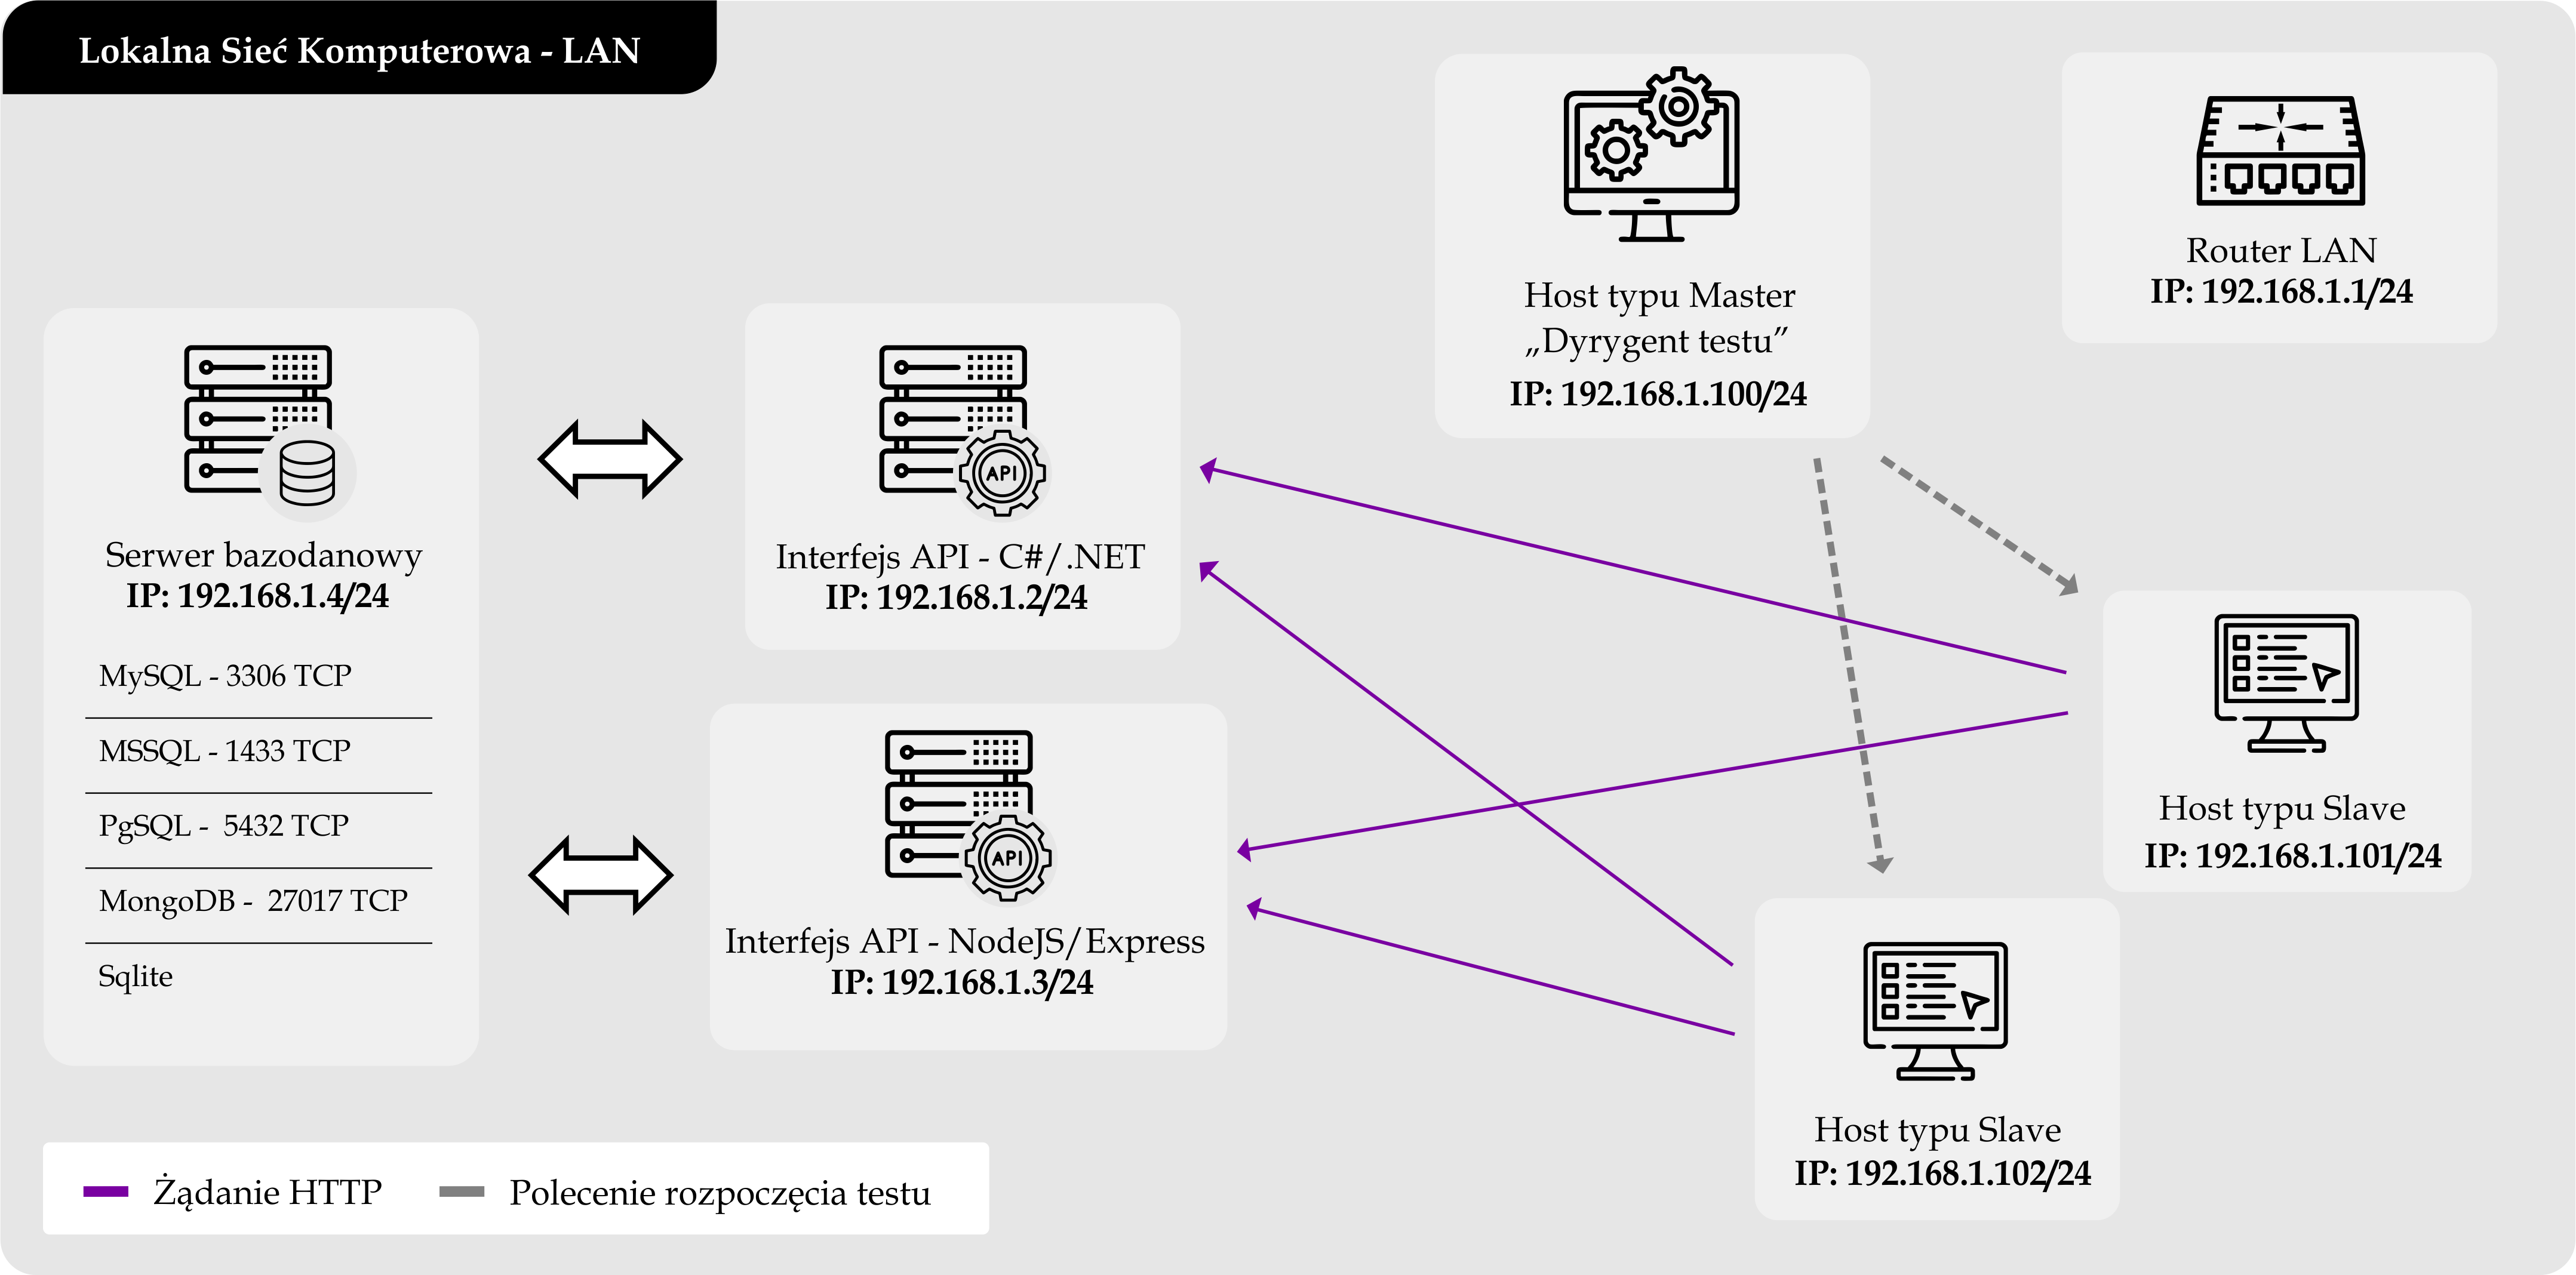
\includegraphics[width=\linewidth]{rys04/topologia-1.png}
    \caption{Konfiguracja pierwsza lokalnej topologii fizycznej środowiska badawczego}
    \label{fig:topologia-1}
\end{figure}

\subsection*{Konfiguracja druga lokalnej topologii fizycznej środowiska badawczego}
\label{sec:lokalne-srodowisko-badawcze-ver-2}
Druga topologia fizyczna środowiska badawczego, dotycząca ewaluacji w obrębie lokalnej sieci komputerowej, zbudowana została na potrzeby badań zaimplementowanych mechanizmów programowania współbieżnego, a także przechowywania odpowiedzi na żądania w ramach pamięci podręcznej.

W omawianej topologii wskazać należy dwa interfejsy programowania aplikacji, których implementacja dokonana została w porównywanych dwóch technologiach programistycznych. Obie usługi sieciowe, komunikują się z pojedyną instancją serwera bazodanowego - w przypadku badania pamięci cache, bądź też nie odwołują się do niego wcale - w przypadku badania efektywności operacji współbieżnych. Spośród urządzeń komunikacyjnych, wykorzystywanych do przeprowadzenia ewaluacji, wyróżnić należy jedno urządzenie typu Master (tzw. Dyrygent testu), a także jednego hosta typu Slave (tzw. generator żądań). Pierwszy z komputerów ma za zadanie przechowywać konfigurację wykonywanego badania, a także dostarczać komendy związane z rozpoczęciem i charakterystyką testu. Drugi host pełni rolę maszyny wytwarzającej i wysyłającej żądania protokołu hipertekstowego, zgodnie z koncepcją nakreśloną przez uzyskany plan ewaluacji. Wszystkie urządzenia znajdują się w obszarze pojedynczej, przewodowej lokalnej sieci komputerowej. Analogicznie do konfiguracji pierwszej, każde łącze przewodowe charakteryzuje się tym samym standardem oraz przepustowością.

Na ilustracji \ref{fig:topologia-2} przedstawiono schemat drugiego wariantu lokalnej topologii fizycznej środowiska badawczego.

\begin{figure}[ht]
    \centering
     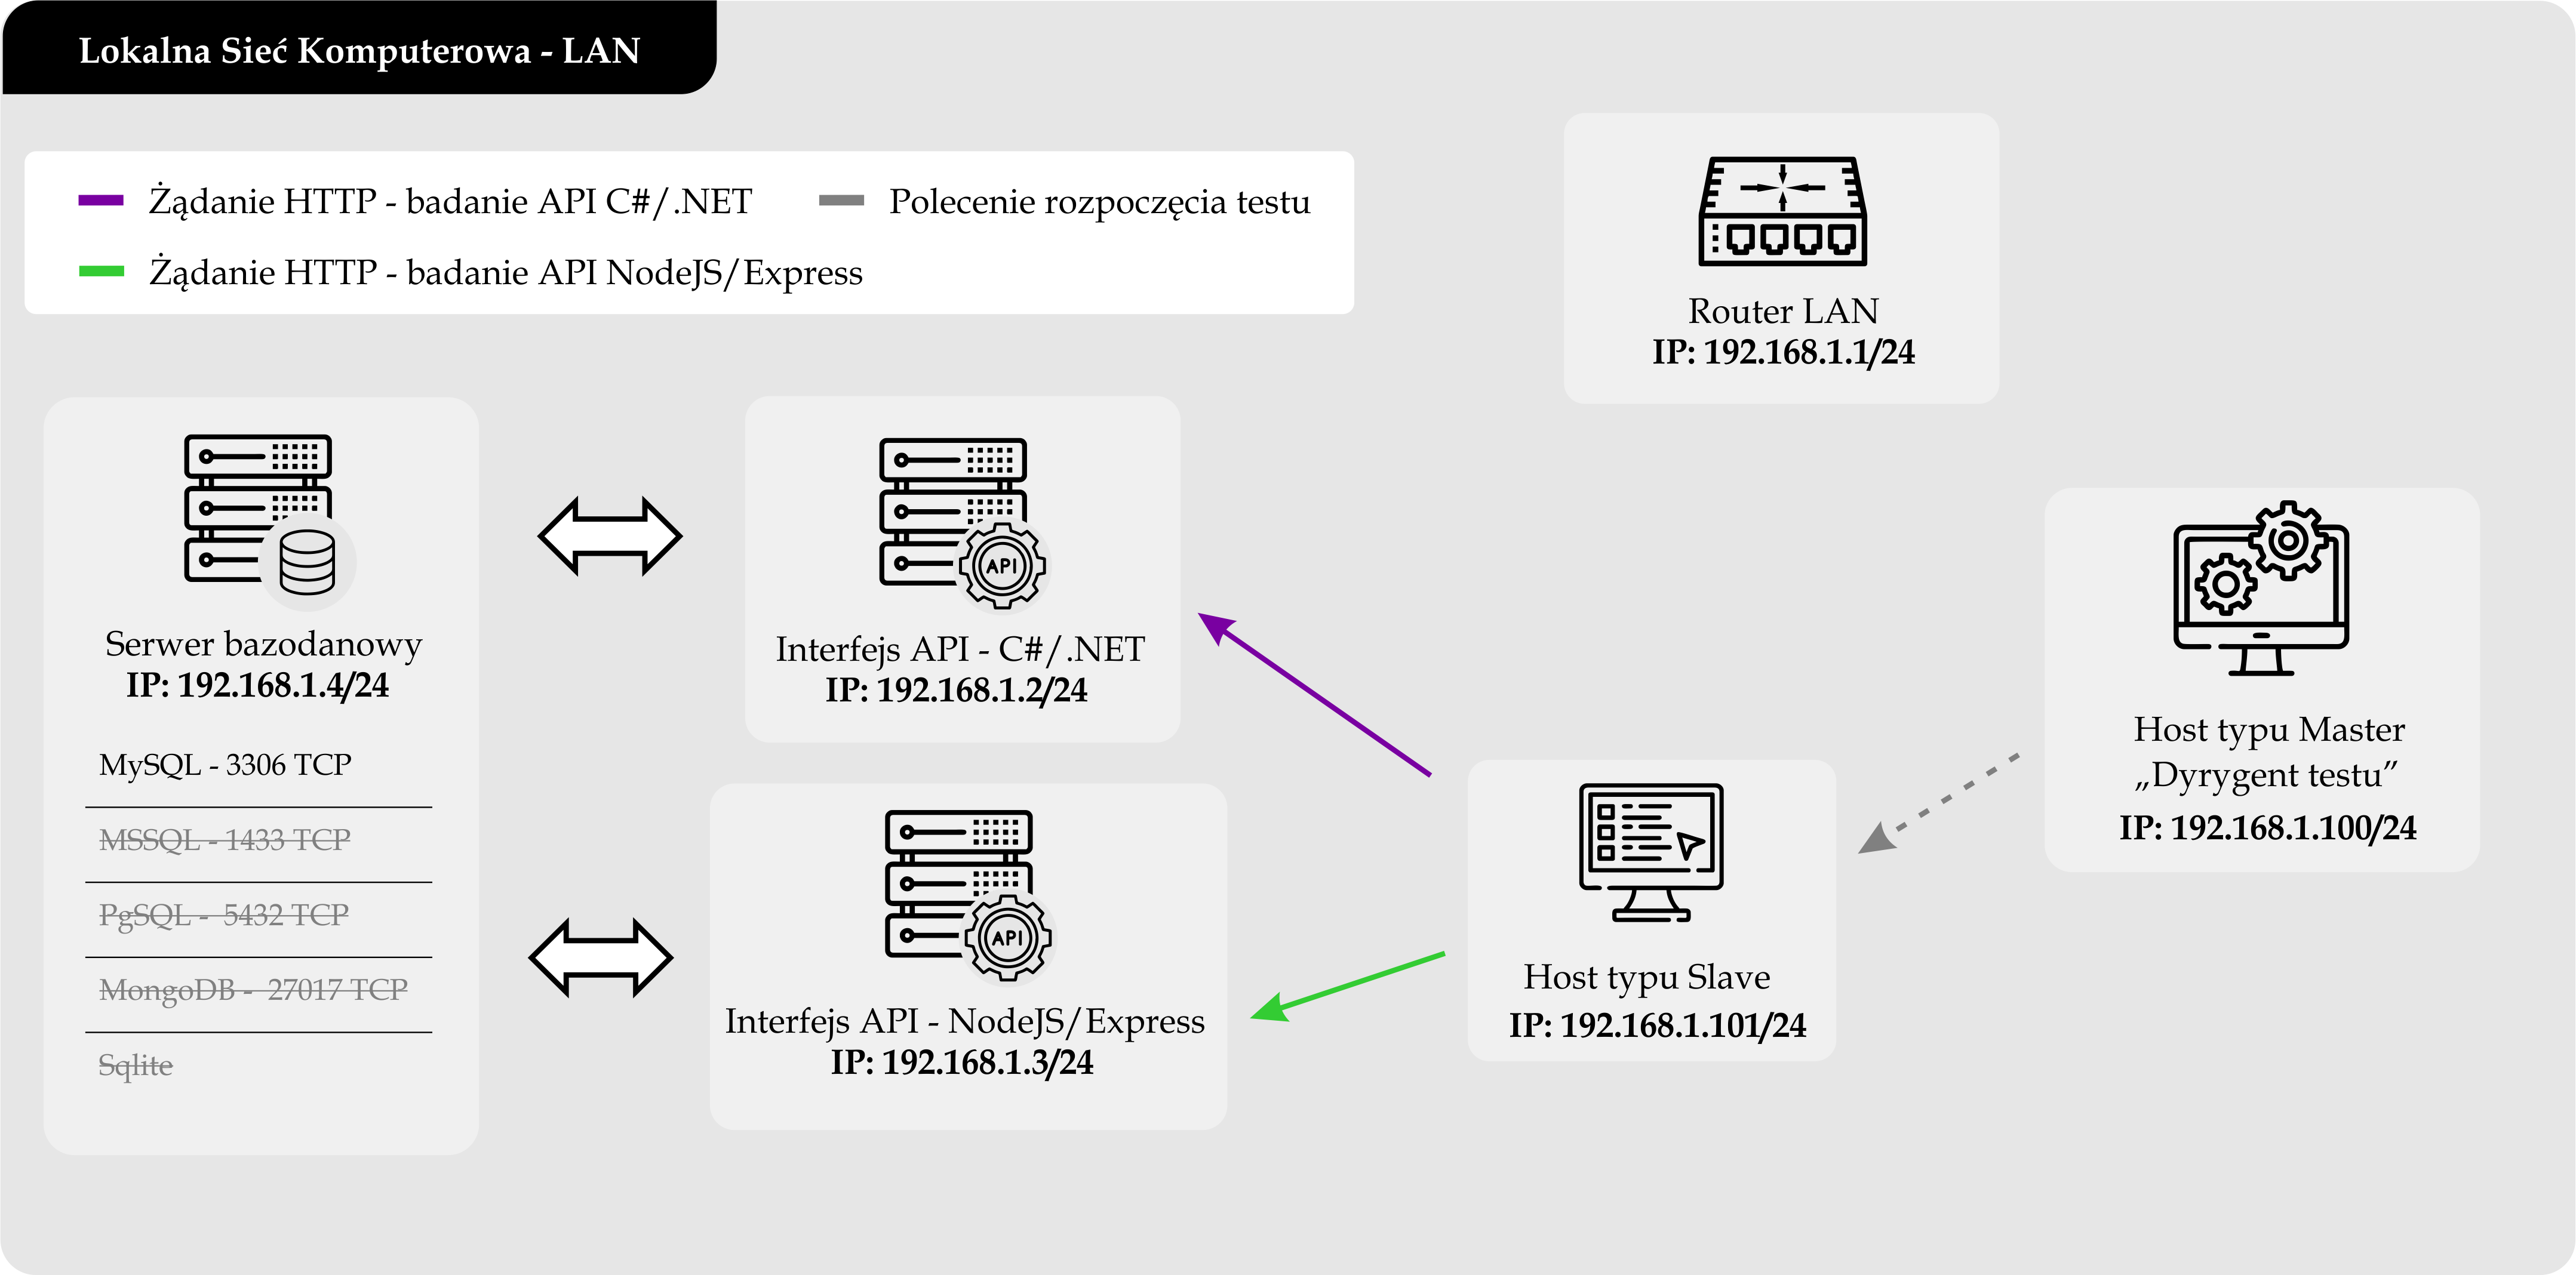
\includegraphics[width=\linewidth]{rys04/topologia-2.png}
    \caption{Konfiguracja druga lokalnej topologii fizycznej środowiska badawczego}
    \label{fig:topologia-2}
\end{figure}

\subsection*{Konfiguracja trzecia lokalnej topologii fizycznej środowiska badawczego}
\label{sec:lokalne-srodowisko-badawcze-ver-3}
Trzecia lokalna topologia fizyczna środowiska badawczego przystosowana została w celu umożliwienia realizacji badań dotyczących wydajności obsługi operacji asynchronicznych.

W schemacie tym, zauważyć można wystąpienie trzech interfejsów programowania aplikacji. Analogicznie do topologii opisanych powyżej, dwa spośród trzech API zaimplementowane są w technologiach będących przedmiotem analizy tej pracy. Trzecia usługa sieciowa, służy do udostępniania zgromadzonych w niej danych, w związku z czym posiada ona tylko i wyłącznie punkty końcowe obsługiwane z wykorzystaniem metody GET. Punkty styku ostatniego z interfejsów dostarczają funkcjonalności pobierania danych o zróżnicowanym rozmiarze.

Ponadto, zbieżnie do konfiguracji pierwszej lokalnego środowiska badawczego, wyszczególnić możemy dwa urządzenia końcowe w roli generatorów żądań, oraz jednego hosta działającego w trybie "Dyrygenta testu". Należy podkreślić, że ewaluacje dotyczące każdej z technologii, zarówno w scenariuszach badawczych wykorzystujących tę, jaki i pozostałe topologie, wykonywane są w odrębnych chwilach czasu. Implikuje to fakt, że połączenie pomiędzy hostem badającym, interfejsem badanym, a także interfejsem pomocniczym jest aktywne tylko dla aktualnie badanego rozwiązania technologicznego.

Poza interfejsami programowania aplikacji oraz urządzeniami końcowymi wskażać należy urządzenie sieciowe, jakim jest przewodowy router LAN, który łączy wszystkie elementy topologii w ramach pojedynczej sieci LAN. Standard oraz przepustowość wykorzystywanych łączy pozostaje niezmienna względem pierwszej oraz drugiej z topologii fizycznych.

Na ilustracji \ref{fig:topologia-3} przedstawiono schemat trzeciego wariantu lokalnej topologii fizycznej środowiska badawczego.

\begin{figure}[ht]
    \centering
     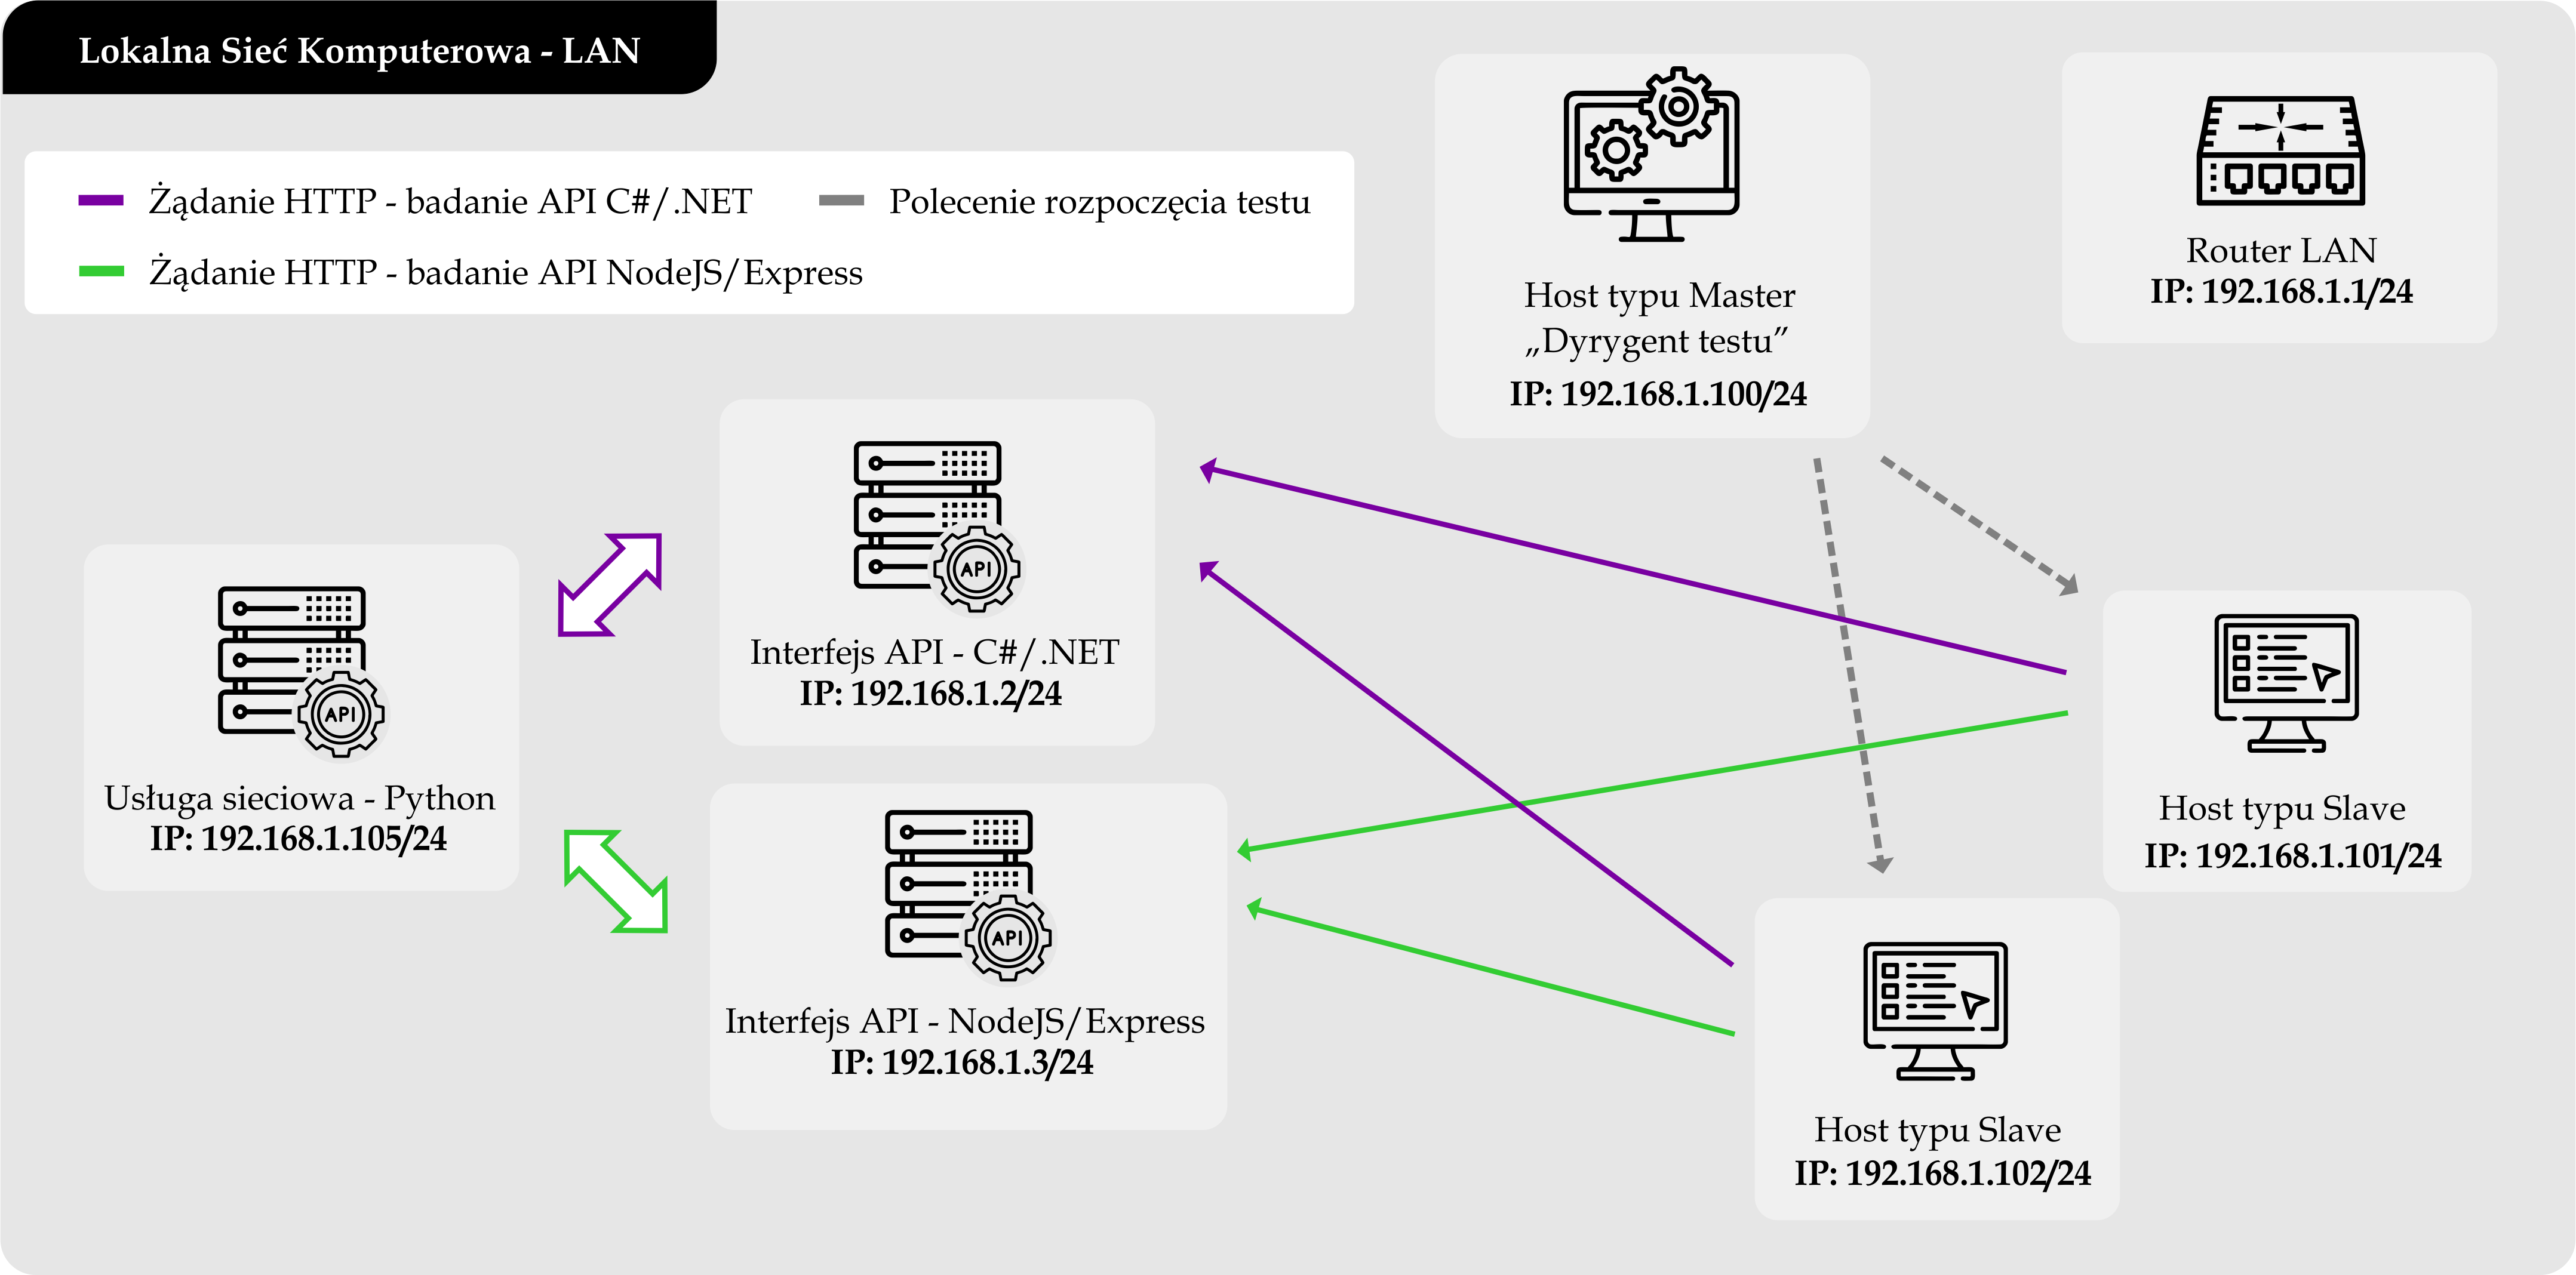
\includegraphics[width=\linewidth]{rys04/topologia-3.png}
    \caption{Konfiguracja trzecia lokalnej topologii fizycznej środowiska badawczego}
    \label{fig:topologia-3}
\end{figure}

\subsection*{Konfiguracja czwarta lokalnej topologii fizycznej środowiska badawczego}
\label{sec:lokalne-srodowisko-badawcze-ver-4}
Ostatnia z lokalnych topologii fizycznych środowiska badawczego zbudowana została w kontekście przeprowadzenia badania efektywności interfejsów programowania aplikacji w związku z zastosowaniem wzorca podziału odpowiedzialności.

Wykorzystanie tego wzorca, umożliwia separację zarówno modeli danych, jak i również fizycznych struktur bazodanowych. Dlatego też, w ramach omawianej topologii zdecydowano się na wprowadzenie dwóch oddzielnych serwerów baz danych. Serwer bazy danych wykorzystywany do zapisu implementuje operację replikacji transakcyjnej dzięki czemu, po wykonaniu zapisu do jednego źródła danych, zapisane informacje są automatycznie przenoszone do drugiej z baz. W ramach połączenia z serwerem bazodanowym wykorzystywanym do odczytu, po stronie interfejsów programowania aplikacji dokonano przystosowania modelu danych.

Poza serwerami danych, w ramach topologii wyróżnić należy dwa porównywane interfejsy programowania aplikacji, a także zbiór trzech urządzeń końcowych. Dwa spośród nich pełnią rolę generatorów żądań, natomiast trzeci host pracuje w trybie "dyrygenta testu". Wszystkie z urządzeń połączone są w obrębie lokalnej sieci komputerowej do urządzenia sieciowego którym jest router LAN.

Na ilustracji \ref{fig:topologia-5} przedstawiono schemat czwartego wariantu lokalnej topologii fizycznej środowiska badawczego.

\clearpage

\begin{figure}[ht]
    \centering
     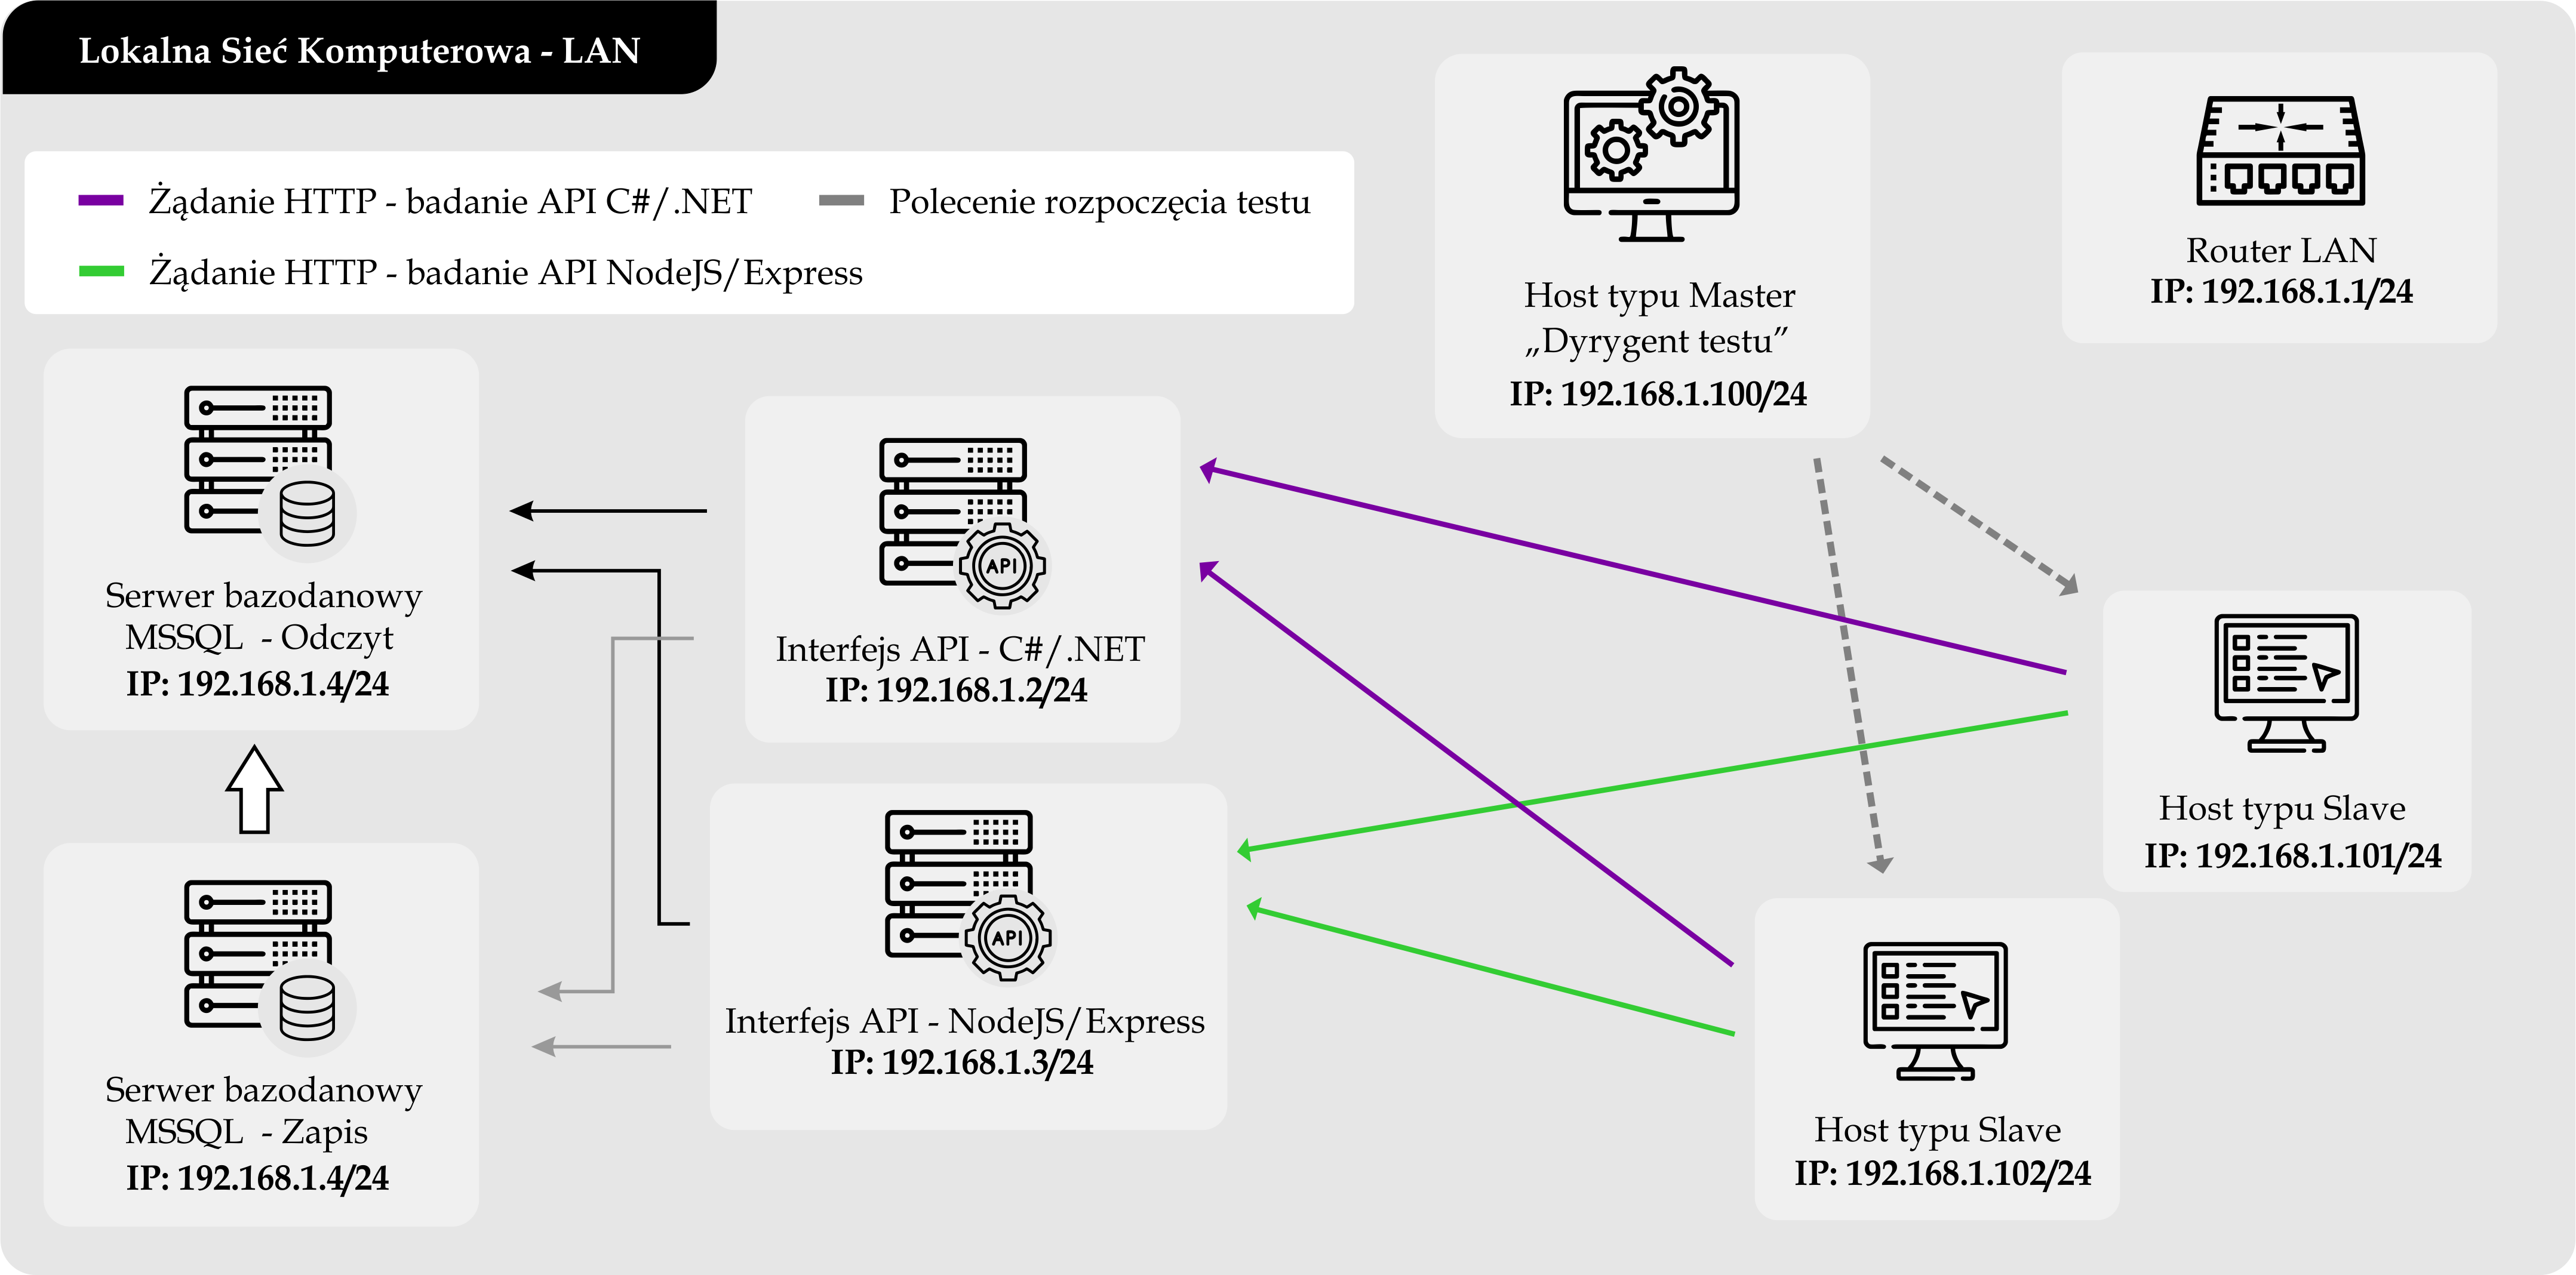
\includegraphics[width=\linewidth]{rys04/topologia-5.png}
    \caption{Konfiguracja czwarta lokalnej topologii fizycznej środowiska badawczego}
    \label{fig:topologia-5}
\end{figure}

\subsection*{Konfiguracja pierwsza rozległej topologii fizycznej środowiska badawczego}
\label{sec:rozproszone-srodowisko-badawcze-ver-1}
Konfiguracja topologii fizycznej dla rozproszonego środowiska badawczego, stworzona została w celu wykonania badań dotyczących efektywności działania interfejsów programowania aplikacji uruchamianych na odmiennych platformach chmurowych.

W tym przypadku, wyodrębnić należy dwa obszary, zawierające urządzenia w kontekście których przeprowadzana jest ewaluacja. Pierwszy obszar to lokalna sieć komputerowa, w której ulokowane zostały urządzenia końcowe odpowiedzialne za przechowywanie konfiguracji badania, a także generowanie żądań w kierunku API. W drugim obszarze zaś, nazwanym rozległą siecią komputerową uruchomione są platformy chmurowe, wewnątrz których działają interfejsy programowania aplikacji oraz serwery bazodanowe. Systemy internetowe zaimplementowane w odrębnych technologiach, przechowywane są na oddzielnych platformach chmurowych i nie są one ze sobą w żaden sposób skomunikowane. Zauważyć należy również fakt, że obie platformy chmurowe znajdują się w różnych lokalizacjach geograficznych. Stwierdzenia te, wymuszają modyfikację sposobu pozyskiwania pomiarów żądań, poprzez przeniesienie odpowiedzialności za wyliczenie czasu wykonywania operacji na interfejsy programowania aplikacji. Pomimo tego, niezbędnym jest posiadania urządzenia generującego żądania zgodnie z określoną charakterystyką. Dlatego też, wewnątrz obszaru lokalnego wskazać możemy dwa urządzenia końcowe, których rolą, podobnie do urządzeń końcowych zawartych we wszystkich poprzednich topologii fizycznych, jest generowanie żądań, oraz koordynowanie przeprowadzanego badania.

Na ilustracji \ref{fig:topologia-4} przedstawiono schemat pierwszego wariantu rozległej topologii fizycznej środowiska badawczego.

\clearpage

\begin{figure}[ht]
    \centering
     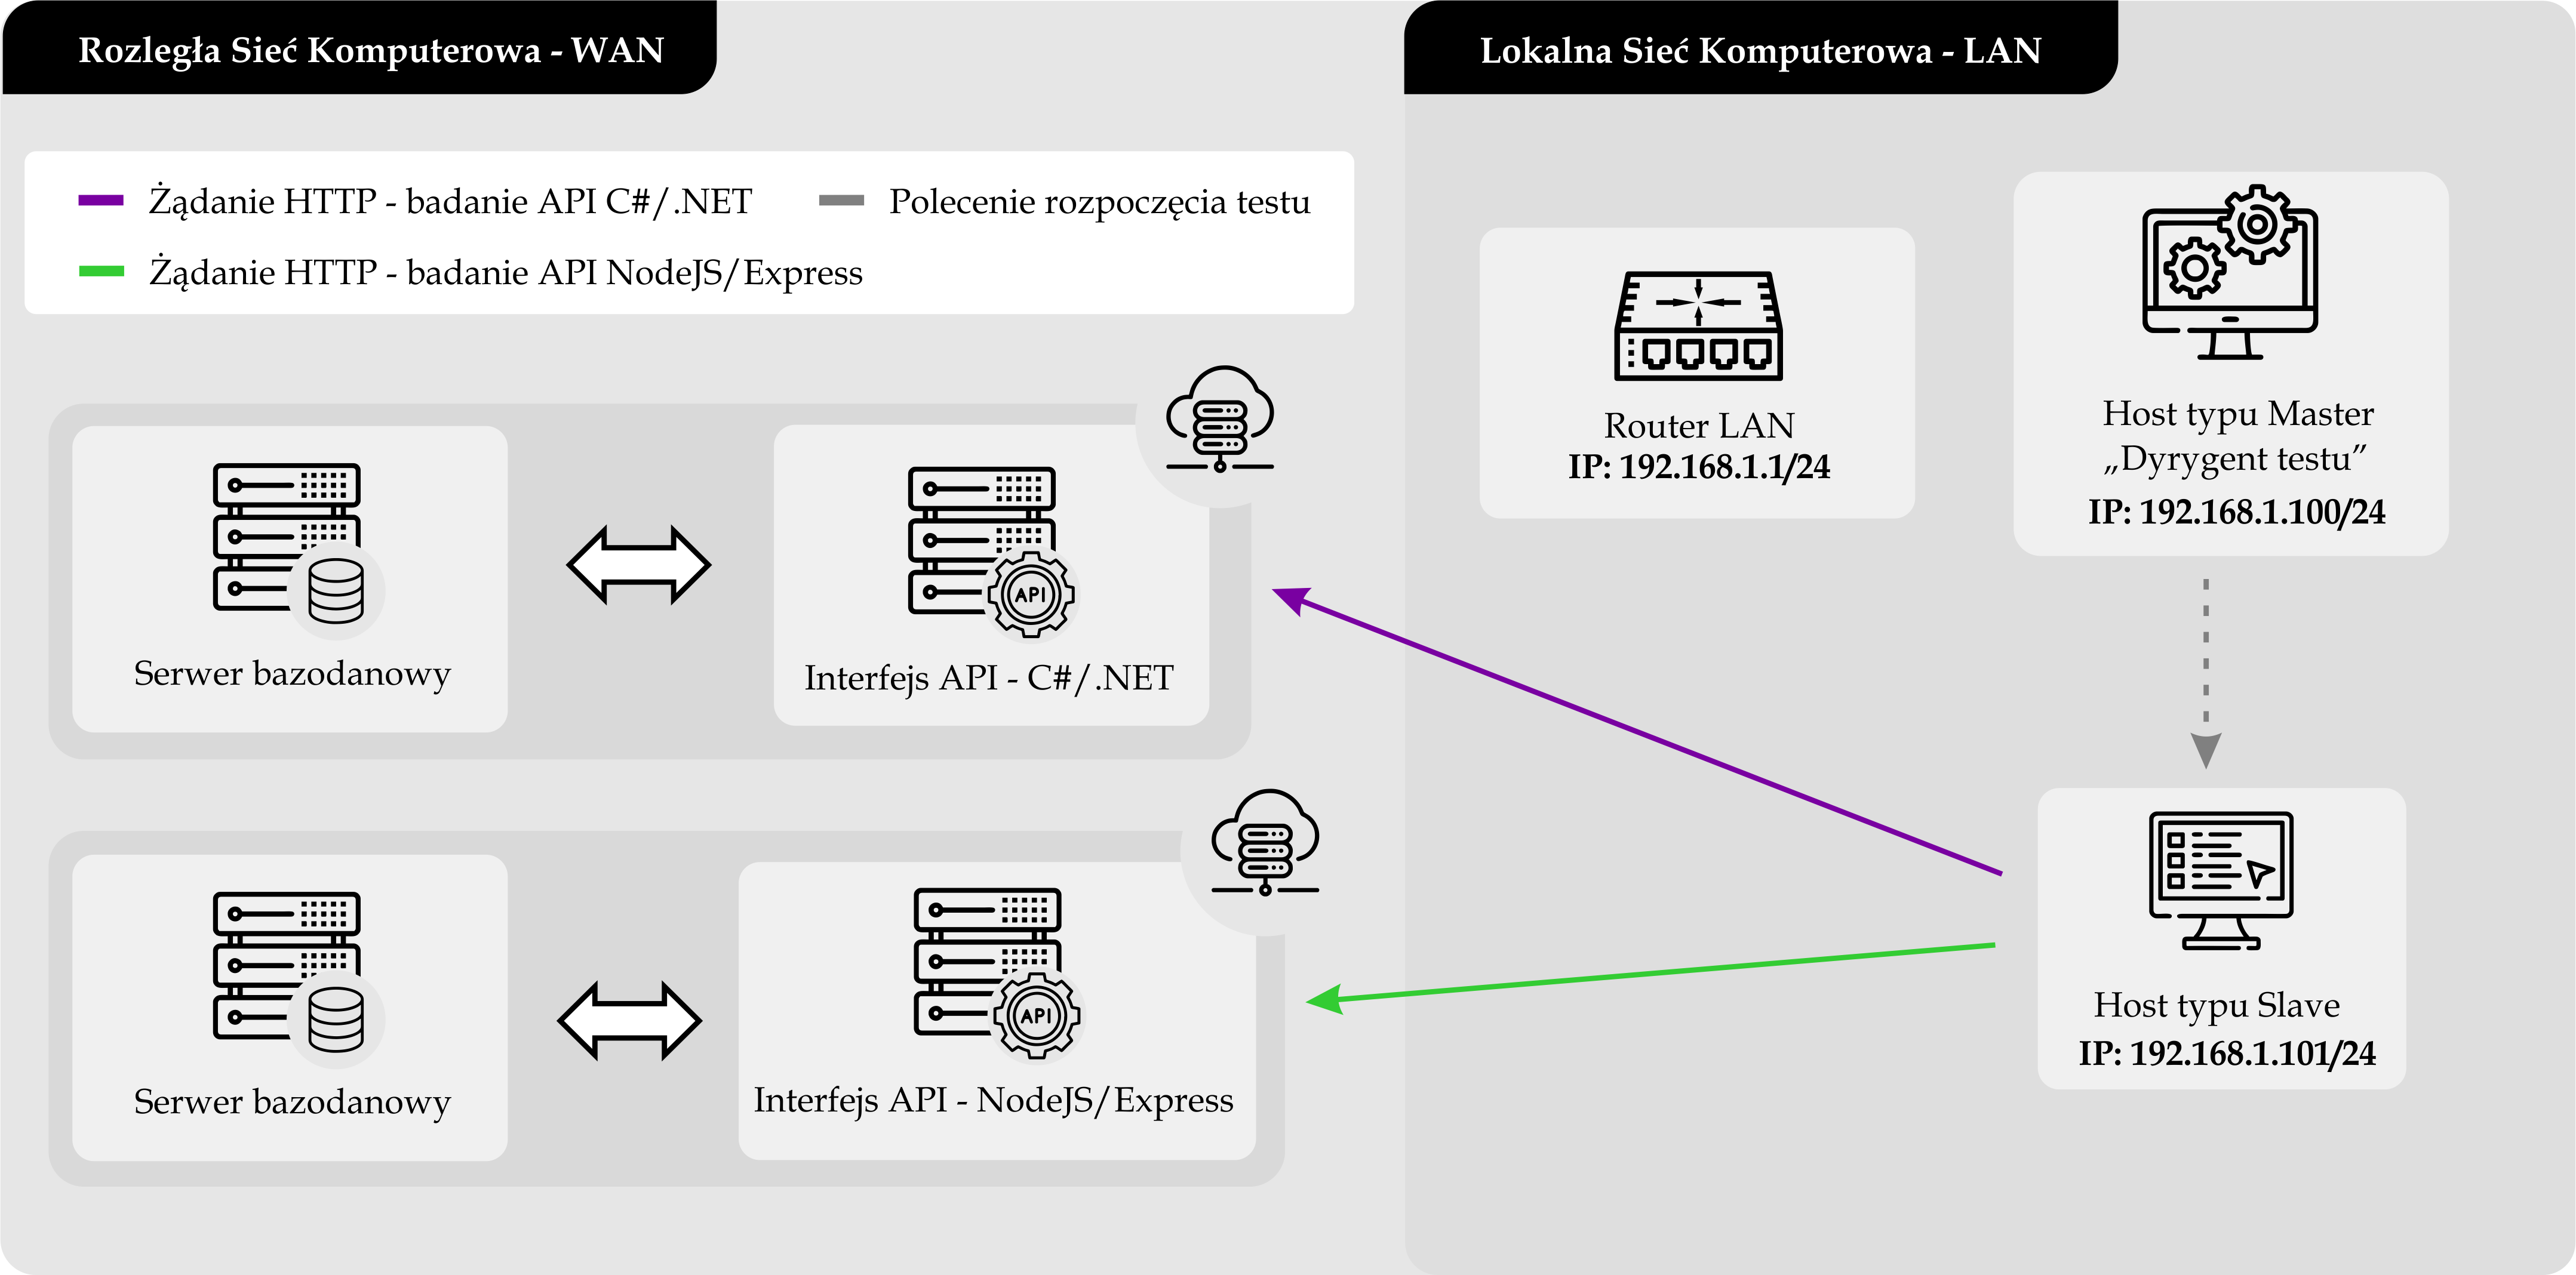
\includegraphics[width=\linewidth]{rys04/topologia-4.png}
    \caption{Konfiguracja pierwsza rozległej topologii fizycznej środowiska badawczego}
    \label{fig:topologia-4}
\end{figure}

\section{Budowa interfejsów programowania aplikacji}
\subsection*{Ogólna funkcjonalność interfejsów programowania aplikacji}
Niezależnie od rozważanej technologii, interfejsy programowania aplikacji implementowane w celu przeprowadzania badań zawartych w ramach niniejszej pracy magisterskiej, dostarczają funkcjonalności obsługi lokalu restauracyjnego. W obrębie omawianych aplikacji zdefiniować można konta użytkowników należących do jednej z pięciu ról pracowniczych. Wyróżnić należy stanowiska: administratora systemu, zarządcy przedsiębiorstwem, kierownika sali, kucharza, a także kelnera. Użytkownicy dysponujący jedną z wymienionych ról mogą korzystać z określonego zestawu funkcjonalności, który determinowany jest poziomem uprawnień zależnych od stanowiska. Przed wywołaniem funkcjonalności systemu, każdy z użytkowników musi zostać uwierzytelniony, a także autoryzowany. Uwierzytelnienie polega na odwołaniu się do punktu końcowego logowania i podaniu swoich danych poświadczeń. Jeżeli dane poświadczeń wskazują na konkretnego użytkownika API, w odpowiedzi zwracany jest token uwierzytelniający, który musi zostać następnie dołączony do nagłówka każdego z wywoływanych żądań. Proces autoryzacji odbywa się na poziomie funkcji warstwy pośredniczącej \textit{(ang. Middleware)}, tuż przed rozpoczęciem wykonywania kodu metody klasy kontrolera.

W kontekście funkcjonalności tworzonych usług sieciowych wymienić należy:
\begin{itemize}
    \item definiowanie oraz zarządzanie strukturą lokalu restauracyjnego (zarządzanie pomieszczeniami lokalu, określanie układu stolików wewnątrz pojedynczego pomieszczenia)
    \item obsługa procesu zamównienia (zarządzanie rachunkami, daniami, statusami przetwarzania posiłków, a także dyspozycjami klientów)
    \item zarządzanie gospodarką magazynową lokalu restauracyjnego (obserwacja stanów ilościowych w kontekście produktu, obsługa danych produktu, definiowanie kategorii produktowych).
\end{itemize}

Dodatkowe funkcje systemu, nie związane z przeprowadzaniem operacji typu CRUD, takie jak wdrożenie metody wyznaczania trasy dla dostarczania zamówień poprzez implementację algorytmu dla symetrycznego problemu komiwojażera, opisane zostały w następnych sekcjach niniejszego rozdziału.
\subsection*{Interfejs API realizujący operacje CRUD stworzony z wykorzystaniem technologii C\#/.NET}
Omawiany interfejs programowania aplikacji zaimplementowany został w języku C\#, z zastosowaniem środowiska uruchomieniowego .NET w wersji piątej. Usługa sieciowa, o której mowa w niniejszym podrozdziale, stanowi złożenie dwóch składowych. Pierwszą z nich jest program, którego zadaniem jest dostarczenie definicji oraz obsługa określonych poleceń klienta, wydanych w postaci żądań protokołu hipertekstowego. Ściśle rzecz ujmując, to właśnie ten program należy określić terminem interfejsu programowania aplikacji. Jako drugą składową natomiast, wskazać należy serwer warstwy aplikacji, pozwalający na obsługę komunikacji pomiędzy usługą sieciową a urządzeniami z zewnątrz. Serwerem wykorzystanym w ramach zaimplementowanej usługi sieciowej jest otwartoźródłowe oprogramowanie Kestrel.

W celu powiązania metod operujących na wewnętrznym modelu danych z fizycznymi strukturami bazodanowymi wykorzystano maper obiektowo-relacyjny Entity Framework Core w wersji drugiej dla relacyjnych systemów baz danych, a także narzędzie Mongoose dla nierelacyjnej bazy danych MongoDB.

Utworzone w języku C\# rozwiązanie złożone jest z pięci projektów powiązanych pomiędzy sobą zależnościami. Pierwszy z projektów zawiera klasy kontrolerów, dokumenty json globalnych właściwości usługi w określonych środowiskach, punkt startowy programu, a także klasę konfiguracji dla wszystkich definiowanych w obrębie całego rozwiązania usług. W projekcie tym, można uzyskać dostęp do struktur programistycznych, definiowanych we wszystkich pozostałych fragmentach rozwiązania.

Drugi z projektów, stworzony został z myślą przechowywania kodu źródłowego związanego z przetwarzaniem logiki biznesowej programu. Zdefiniowane zostały tu klasy serwisów, metody rozszerzeń dla typów języka, obiekt parametrów paginacji, klasy transferu danych \textit{(ang. Data Transfer Objects)}, a także prodecury generowania opowiedzi dla użytkownika. Od projektu tego, zależne są wszystkie fragmenty rozwiązania z wyłączeniem pierwszego z omawianych.

Na równorzędnym poziomie hierarchii, zdefiniowany został projekt dotyczący obsługi operacji związanych z bezpieczeństwem interfejsu API. Wyróżnić możemy tutaj klasę generatora tokenu uwierzytelniającego, a także metodę dostępu do właściwości identyfikujących użytkownika poprzez zawartość kontekstu żądania http.

Kolejnym fragmentem rozwiązania stworzonego w języku C\# jest projekt dostępu do danych. W projekcie tym, wskazać należy klasę kontekstu danych, zbiór migracji modelu danych do schematów bazodanowych, klasę propagacji danych początkowych, a także listę metod struktur repozytoriów, które pozwalają na wykonywanie bezpośrednich operacji na wykorzystywanym zbiorze informacji. Omawiany fragment, posiada zależność względem projektu logiki biznesowej.

Ostatnim projektem rozwiązania jest przestrzeń przechowywania klas modelu danych. Fragment ten, nie wprowadza zależności względem jakiegokolwiek z pozostałych projektów i pełni rolę rdzenia aplikacji. Każda z omówinionych powyżej przestrzenii kodu źródłowego posiada dostęp do elementów modelu, jednakże jakiekolwiek operacje na tych danych, wykonywane są tylko i wyłącznie z poziomie klas repozytoriów.

Na ilustracji \ref{fig:struktura-plikow-dotnet} przedstawiono strukturę obiektów wewnątrz poszczególnych fragmentów rozwiązania. Niektóre spośród elementów każdego projektu zostały pominięte na niniejszym rysunku w celu zachowania czytelności omawianej treści.

\begin{figure}[ht]
    \centering
     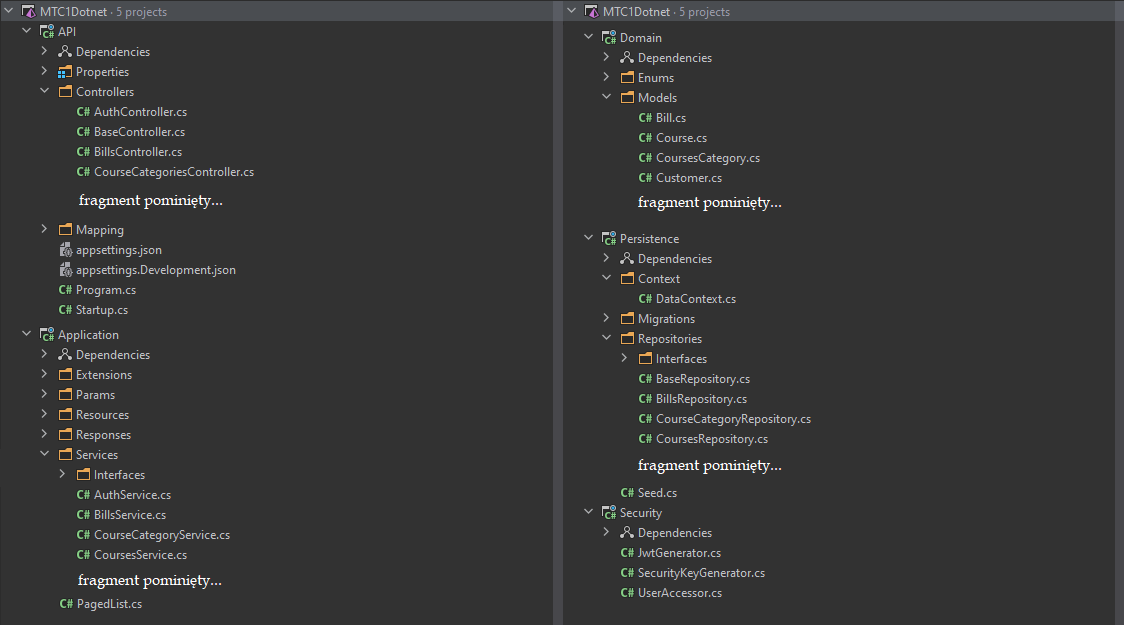
\includegraphics[width=\linewidth]{rys04/struktura-plikow-dotnet.png}
    \caption{Struktura obiektów wewnątrz rozwiązania systemu internetowego zaimplementowanego w języku C\#}
    \label{fig:struktura-plikow-dotnet}
\end{figure}
\subsection*{Interfejs API realizujący operacje CRUD stworzony z wykorzystaniem technologii NodeJS/Express}
Druga z realizacji interfejsu programowania aplikacji napisana została w języku JavaScript, zgodnym ze specyfikacją językową ECMAScript 6. Do implementacji funkcjonalności omawianej usługi sieciowej, wykorzystano bibliotekę ExpressJS w wersji czwartej, a całość oprogramowania uruchomiono na serwerze wykorzystującym natywne moduły platformy uruchomieniowej NodeJS.

W celu powiązania metod operujących na wewnętrznym modelu danych z fizycznymi strukturami bazodanowymi wykorzystano maper obiektowo-relacyjny Prisma w wersji pierwszej dla relacyjnych systemów baz danych, a także narzędzie Mongoose dla nierelacyjnej bazy danych MongoDB.

W przeciwieństwie do rozwiązania utworzonego przy wykorzystaniu technologii firmy Microsoft, schemat struktur programistycznych interfejsu programowania aplikacji opartego o JavaScript cechuje się znacząco niższym poziomem skomplikowania. Całość oprogramowania przechowywana jest w ramach pojedynczego projektu, wewnątrz którego podział struktur programistycznych ze względu na odpowiedzialności dokonany został na poziomie folderów.

Punktem startowym aplikacji, a także miejscem definicji podstawowej konfiguracji elementów usługi sieciowej jest skryptowy plik o nazwie \textit{app.js}. W pliku tym, określono wartości dla zmiennych globalnych dotyczących ścieżki podstawowej w aplikacji, czy też klucza tajnego wykorzystywanego do wyliczania tokenu uwierzytelniania. Ponadto, określono funkcje pośredniczące wykonujące się przed rozpoczęciem zadanej funkcji modułu kontrolera. Plik \textit{app.js}, zawiera także informacje dotyczące lokalizacji modułów, odpowiadających za obsługę punktów końcowych dla określonej ścieżki wywołania.

Poza plikiem startowym interfejsu programowania aplikacji wskazać należy foldery, przechowujące moduły odpowiedzialne za poprawną pracę całości aplikacji. Pierwszy z folderów o nazwie \textit{controllers}, stanowi zbiór modułów zawierających funkcje obsługujące każdy z zaimplementowanych punktów końcowych. Funkcje te, odwołują się do fragmentów oprogramowania realizujących operacje logiki biznesowej, które to fragmenty umieszczone są w folderze \textit{services}. Analogiczne odwołanie ma miejsce w kontekście modułów serwisów a funkcji operujących na danych. Funkcje te, znaleźć można w folderze \textit{repositories}. Ponadto, wyróżnić należy katalog \textit{errors}, przechowujący kod źródłowy dotyczący przetwarzania błędów dla każdej z logicznych warstw interfejsu, katalog \textit{helpers} w ramach którego zdefiniowane zostały funkcje pomocnicze, a także folder \textit{prisma}, zawierający w sobie pliki migracji oraz dokument definicji schematu modelu danych.

Na ilustracji \ref{fig:struktura-plikow-nodejs} przedstawiono strukturę obiektów wewnątrz poszczególnych fragmentów rozwiązania. Niektóre spośród elementów każdego projektu zostały pominięte na niniejszym rysunku w celu zachowania czytelności omawianej treści.

\begin{figure}[ht]
    \centering
     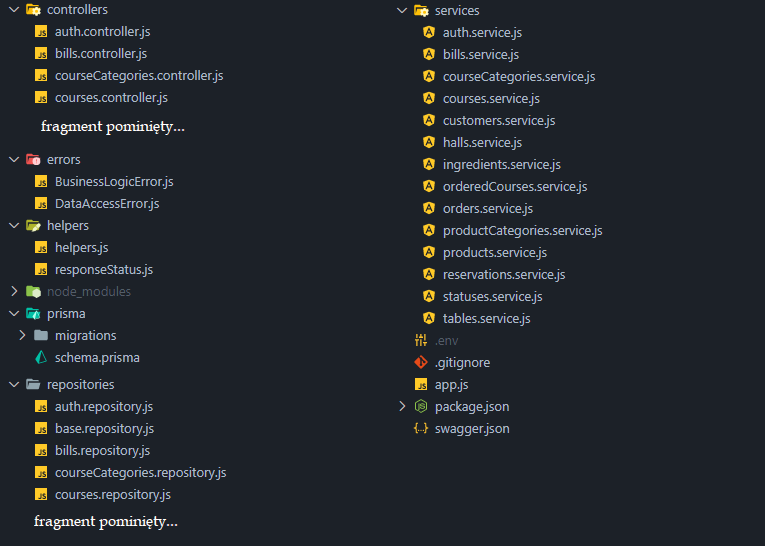
\includegraphics[width=\linewidth]{rys04/struktura-plikow-nodejs.png}
    \caption{Struktura obiektów wewnątrz rozwiązania systemu internetowego zaimplementowanego w języku JavaScript}
    \label{fig:struktura-plikow-nodejs}
\end{figure}

\subsection*{Algorytm metaheurystyczny dla symetrycznego problemu komiwojażera}
\label{label:algorytm-genetyczny}
W celu realizacji badania wydajności przetwarzania operacji współbieżnych zdecydowano się na implementację algorytmu metaheurystycznego przeznaczonego do rozwiązywania symetrycznego problemu komiwojażera. Zaimplementowany algorytm, sklasyfikować należy jako heurystykę z rodziny algorytmów genetycznych. Algorytmy te, zaliczane są do przestrzenii schematów ewolucyjnych, których główną koncepcją jest próba przeniesienia procesów, a także zachowań biologicznych obserwowanych w ramach dziedziny genetyki, w obszar definiowania oraz realizacji algorytmów. 

Należyte przedstawienie procesu wykonania algorytmu genetycznego wymaga wprowadzenia odpowiedniej terminologii. Terminologia ta, podobnie jak wspomniane uprzednio obserwowane procesy biologiczne, została zaczerpnięta z dziedziny genetyki. Podstawowym pojęciem, który należy wyróżnić w ramach wprowadzanych definicji jest chromosom. W kontekście algorytmu genetycznego jest on iterpretowany jako pojedynczy element rozwiązania określonego problemu optymalizacyjnego (w tym przypadku, pojedyncza lokalizacja która ma zostać odwiedzona przez osobę przemierzającą trasę). Wszystkie spośród permutacji zbioru chromosomów, przy założeniu, że liczba elementów permutacji równa jest wielkości zbioru, identyfikowane są jako osobniki, w ramach określonej populacji. Każdy z osobników populacji może zostać poddawany modyfikacji jego kodu genetycznego (zmiany jego chromosomów), poprzez zdefiniowane operacje krzyżowania osobników, a także ich mutacji. Ponadto, w celu wyboru najlepszych spośród osobników, wykonywany jest proces selekcji. Proces ten, powiązany jest ściśle z metryką oceny jakości osobnika względem populacji nazywaną funkcją przystosowania.

Na rysunku \ref{fig:algorytm-genetyczny} zilustrowano schemat blokowy algorytmu genetycznego.

\begin{figure}[ht]
    \centering
     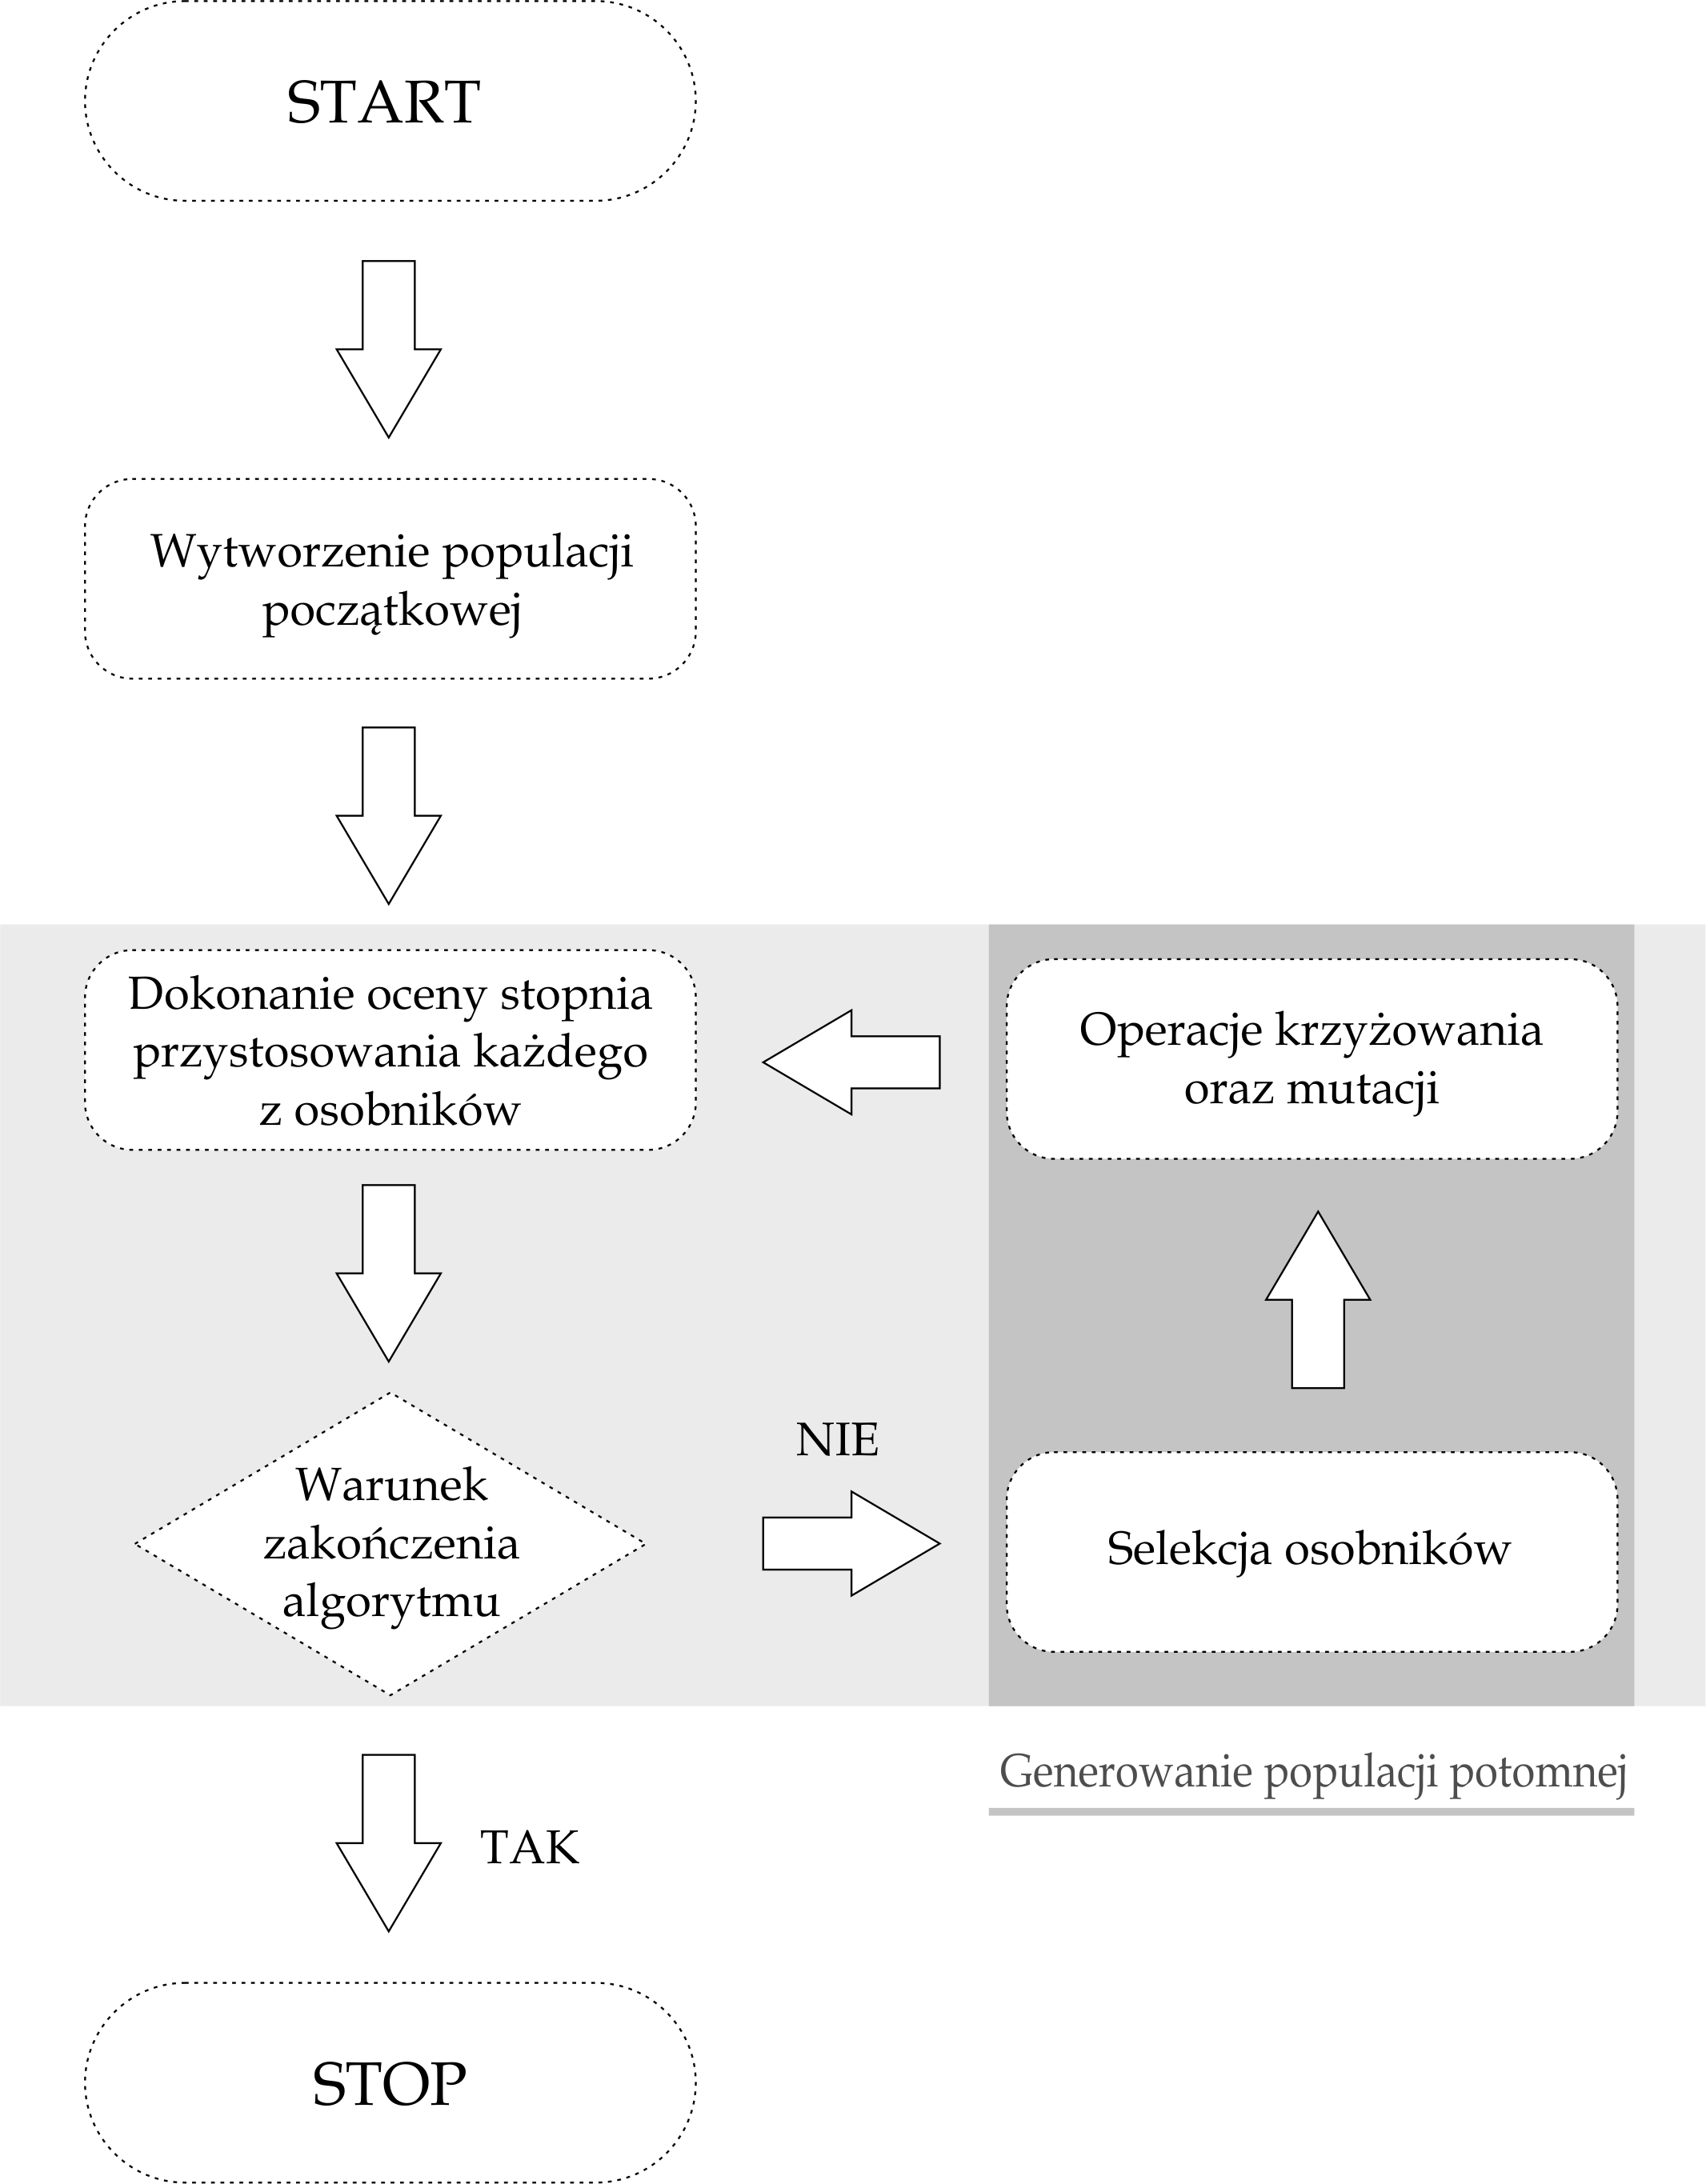
\includegraphics[width=0.6\linewidth]{rys04/algorytm-genetyczny.png}
    \caption{Schemat blokowy algorytmu genetycznego}
    \label{fig:algorytm-genetyczny}
\end{figure}

Implementowane rozwiązanie omawiane w ramach niniejszej pracy dyplomowej cechuje się realizacją funkcji krzyżowania osobników z wykorzystaniem dwóch punktów podziału (tzw. krzyżowanie dwupunktowe), a także dokonaniem mutacji w zależności od przyjętego prawdopodobieństwa. Ponadto, metodę selekcji oparto na technice ruletkowej, wzbogacają technikę tę, o mechanizm zapobiegania zjawisku przedwczesnej zbieżności poprzez kontrolę liczby osobników dominujących w populacji.

W tabeli \ref{tab:hiperparametry-genetyczny} wymieniono hiperparametry zaimplementowanej metaheurystyki genetycznej, a także opisano ich znaczenie w kontekście schematu działania algorytmu.

\begin{table}[htb] \small
\centering
\caption{Wykaz hiperparametrów zaimplementowanego algorytmu genetycznego}
\label{tab:hiperparametry-genetyczny}
\begin{tabularx}{\linewidth}{|X|X|X|} \hline\
    Nazwa parametru & Opis & Wartość domyślna \\ \hline\hline
    Prawdopodobieństwo mutacji osobnika & Parametr definiujący częstość wystąpienia zdarzenia modyfikacji pojedynczego chromosomu w obrębie osobnika & 0,01 \\ \hline
    Prawdopodobieństwo krzyżowania osobników & Parametr definiujący częstość wystąpienia zdarzenia wymiany kodu genetycznego pomiędzy określonymi osobnikami & 1 \\ \hline
    Rozmiar populacji & Liczba osobników poddawanych ewolucji, spośród których ostatecznie wybierane jest rozwiązanie najlepsze & 0,75 * liczba wszystkich rozpatrywanych lokalizacji \\ \hline
    Liczba osobników dominujących w ramach pojedynczej populacji & Rozmiar podgrupy w obrębie pojedynczej populacji, skupiającej w sobie osobników o najwyższych wartościach funkcji przystosowania & 0.25 * rozmiar populacji \\ \hline
    Czas wykonania algorytmu & Przedział czasu określany przez liczbę sekund, w ramach którego wykonywana będzie główna pętla algorytmu & 60 \\ \hline
\hline
\end{tabularx}
\end{table}

Niezależnie od środowiska, w którym implementowany został opisany powyżej algorytm, sposób uruchamiania, przekazywania danych wejściowych, a także format danych wyjściowych jest identyczny. Omawiany algorytm metaheurystyczny dostępny jest z poziomu punktu końcowego określonych interfejsów programowania aplikacji jako żądanie protokołu hipertekstowego dla ścieżki \textit{/api/algorithms/roadPlan} oraz metody HTTP POST. Format danych wejściowych określony został jako tablica obiektów notacji JSON, zawierających właściwości definiujące szerokość i długość geograficzną, a także adres dla pojedynczej lokalizacji. Rezultatem otrzymywanym w ramach odpowiedzi protokołu hipertekstowego jest obiekt zawierający informacje dotyczącą ilorazu uzyskanego wyniku względem wyniku optymalnego, a także liczbę przeprowadzonych w pętli głównej algorytmu. Czas wykonania pojedynczego żądania dla omawianego punktu końcowego wynosi co najmniej 60 sekund.


W odniesieniu do szczegółów implementacyjnych tyczących się języka C\# oraz środowiska uruchomieniowego .NET, wspomnieć należy o wykonaniu kodu źródłowego głównej pętli algorytmu w ramach osobnego wątku. Po zdefiniowaniu wartości hiperparametrów heurystyki, inicjowana jest nowa instancja klasy \textit{Thread}, która przyjmuje w ramach konstruktora metodę wykonawczą (w tym przypadku metodę pętli głównej algorytmu). Następnie, obiekt klasy \textit{Timer}, odlicza czas 60 sekund, w ramach których pętla programu może być wykonana. Po upłynięciu czasu wykonania kodu, wątek algorytmiczny łączony jest z głównym wątkiem wykorzystywanym do przetwarzania żądania, a rezultaty działania algorytmu formułowane są do postaci ciała odpowiedzi protokołu HTTP.  


W ramach interfejsu programowania aplikacji zaimplementowanego w języku JavaScript, sposób przetwarzania współbieżnego różni się w sposób znaczący względem języka C\#. Język JavaScript jest rozwiązaniem które dostarcza mechanizmy przetwarzania tylko i wyłączenie w obrębie pojedynczego wątku procesora. Dlatego też, wspominając o tej właśnie technologii programistycznej nie można stwierdzić, że istnieje możliwość współbieżnego wykonania kodu źródłowego. Przepływ sterowania od momentu wywołania punktu końcowego uwzględnia inicjalizację serwisu realizacji algorytmów, zdefiniowanie hiperparametrów programu, rozpoczęcie wykonania pomiaru czasu, a także uruchomienie pętli głównej algorytmu. Pomiar czasu wykonywany jest za pomocą natywnej struktury programistycznej dostarczanej zarówno w ramach środowiska NodeJS, jaki i implementowanej przez silniki obsługi języka JavaScript w przeglądarkach internetowych (tj. interfejs \textit{Performance}).
\subsection*{Mechanizmy obsługi pamięci podręcznej}
\label{sec:mechanizmy-cache}
Implementacja mechanizmów obsługi pamięci podręcznej wykonana została w oparciu o otwartoźródłowe rozwiązanie \textit{Redis}, dostarczające zarówno strukturę danych pełniącą rolę magazynu wpisów pamięci cache, jak i interfejsy programistyczne służące do ustanowienia połączenia, a także zarządzania zawartością tej struktury. Magazyn pamięci podręcznej Redis uruchomiony został jako autonomiczna usługa sieciowa poprzez wykonanie obrazu \textit{bitnami/redis} w obrębie kontenera \textit{Docker}.

Niezależnie od badanej technologii programistycznej, zaimplementowane mechanizmy pamięci podręcznej są niezależne od określonego punktu końcowego i mogą zostać połączone z dowolną metodą klasy kontrolera, której wynikiem działania jest obiekt odpowiedzi, specyficzny względem wybranego języka. Wykonanie kodu źródłowego związanego z obsługą mechanizmów pamięci podręcznej odbywa się wewnątrz metod pośredniczących \textit{(ang. Middleware)}. Metody te, uzyskują dostęp zarówno do treści żądania wygenerowanego przez aplikację kliencką, jak i odpowiedzi będącej rezultatem działania metody klasy kontrolera. Implikuje to możliwość definiowania identyfikatorów wpisów w pamięci podręcznej dla każdego z wywołanych żądań.

Klucze poszczególnych elementów przechowywanych w pamięci cache składają się ze składowej ścieżki, oraz składowych parametrów. Każdy z fragmentów identyfikatora wpisu rozdzielony jest znakiem średnika, natomiast w obrębie składowej parametru klucz odseparowany jest od wartości znakiem kreski pionowej. Aby zapewnić jednoznaczność wpisu niezależnie od kolejności w jakiej aplikacja kliencka definiuje parametry wewnątrz ciała żądania, poszczególne składowe właściwości są sortowane w kolejności rosnącej według nazwy parametru.

Na ilustracji \ref{fig:cache-klucz} zaprezentowano format klucza wpisu przechowywanego w pamięci podręcznej.

\begin{figure}[ht]
    \centering
     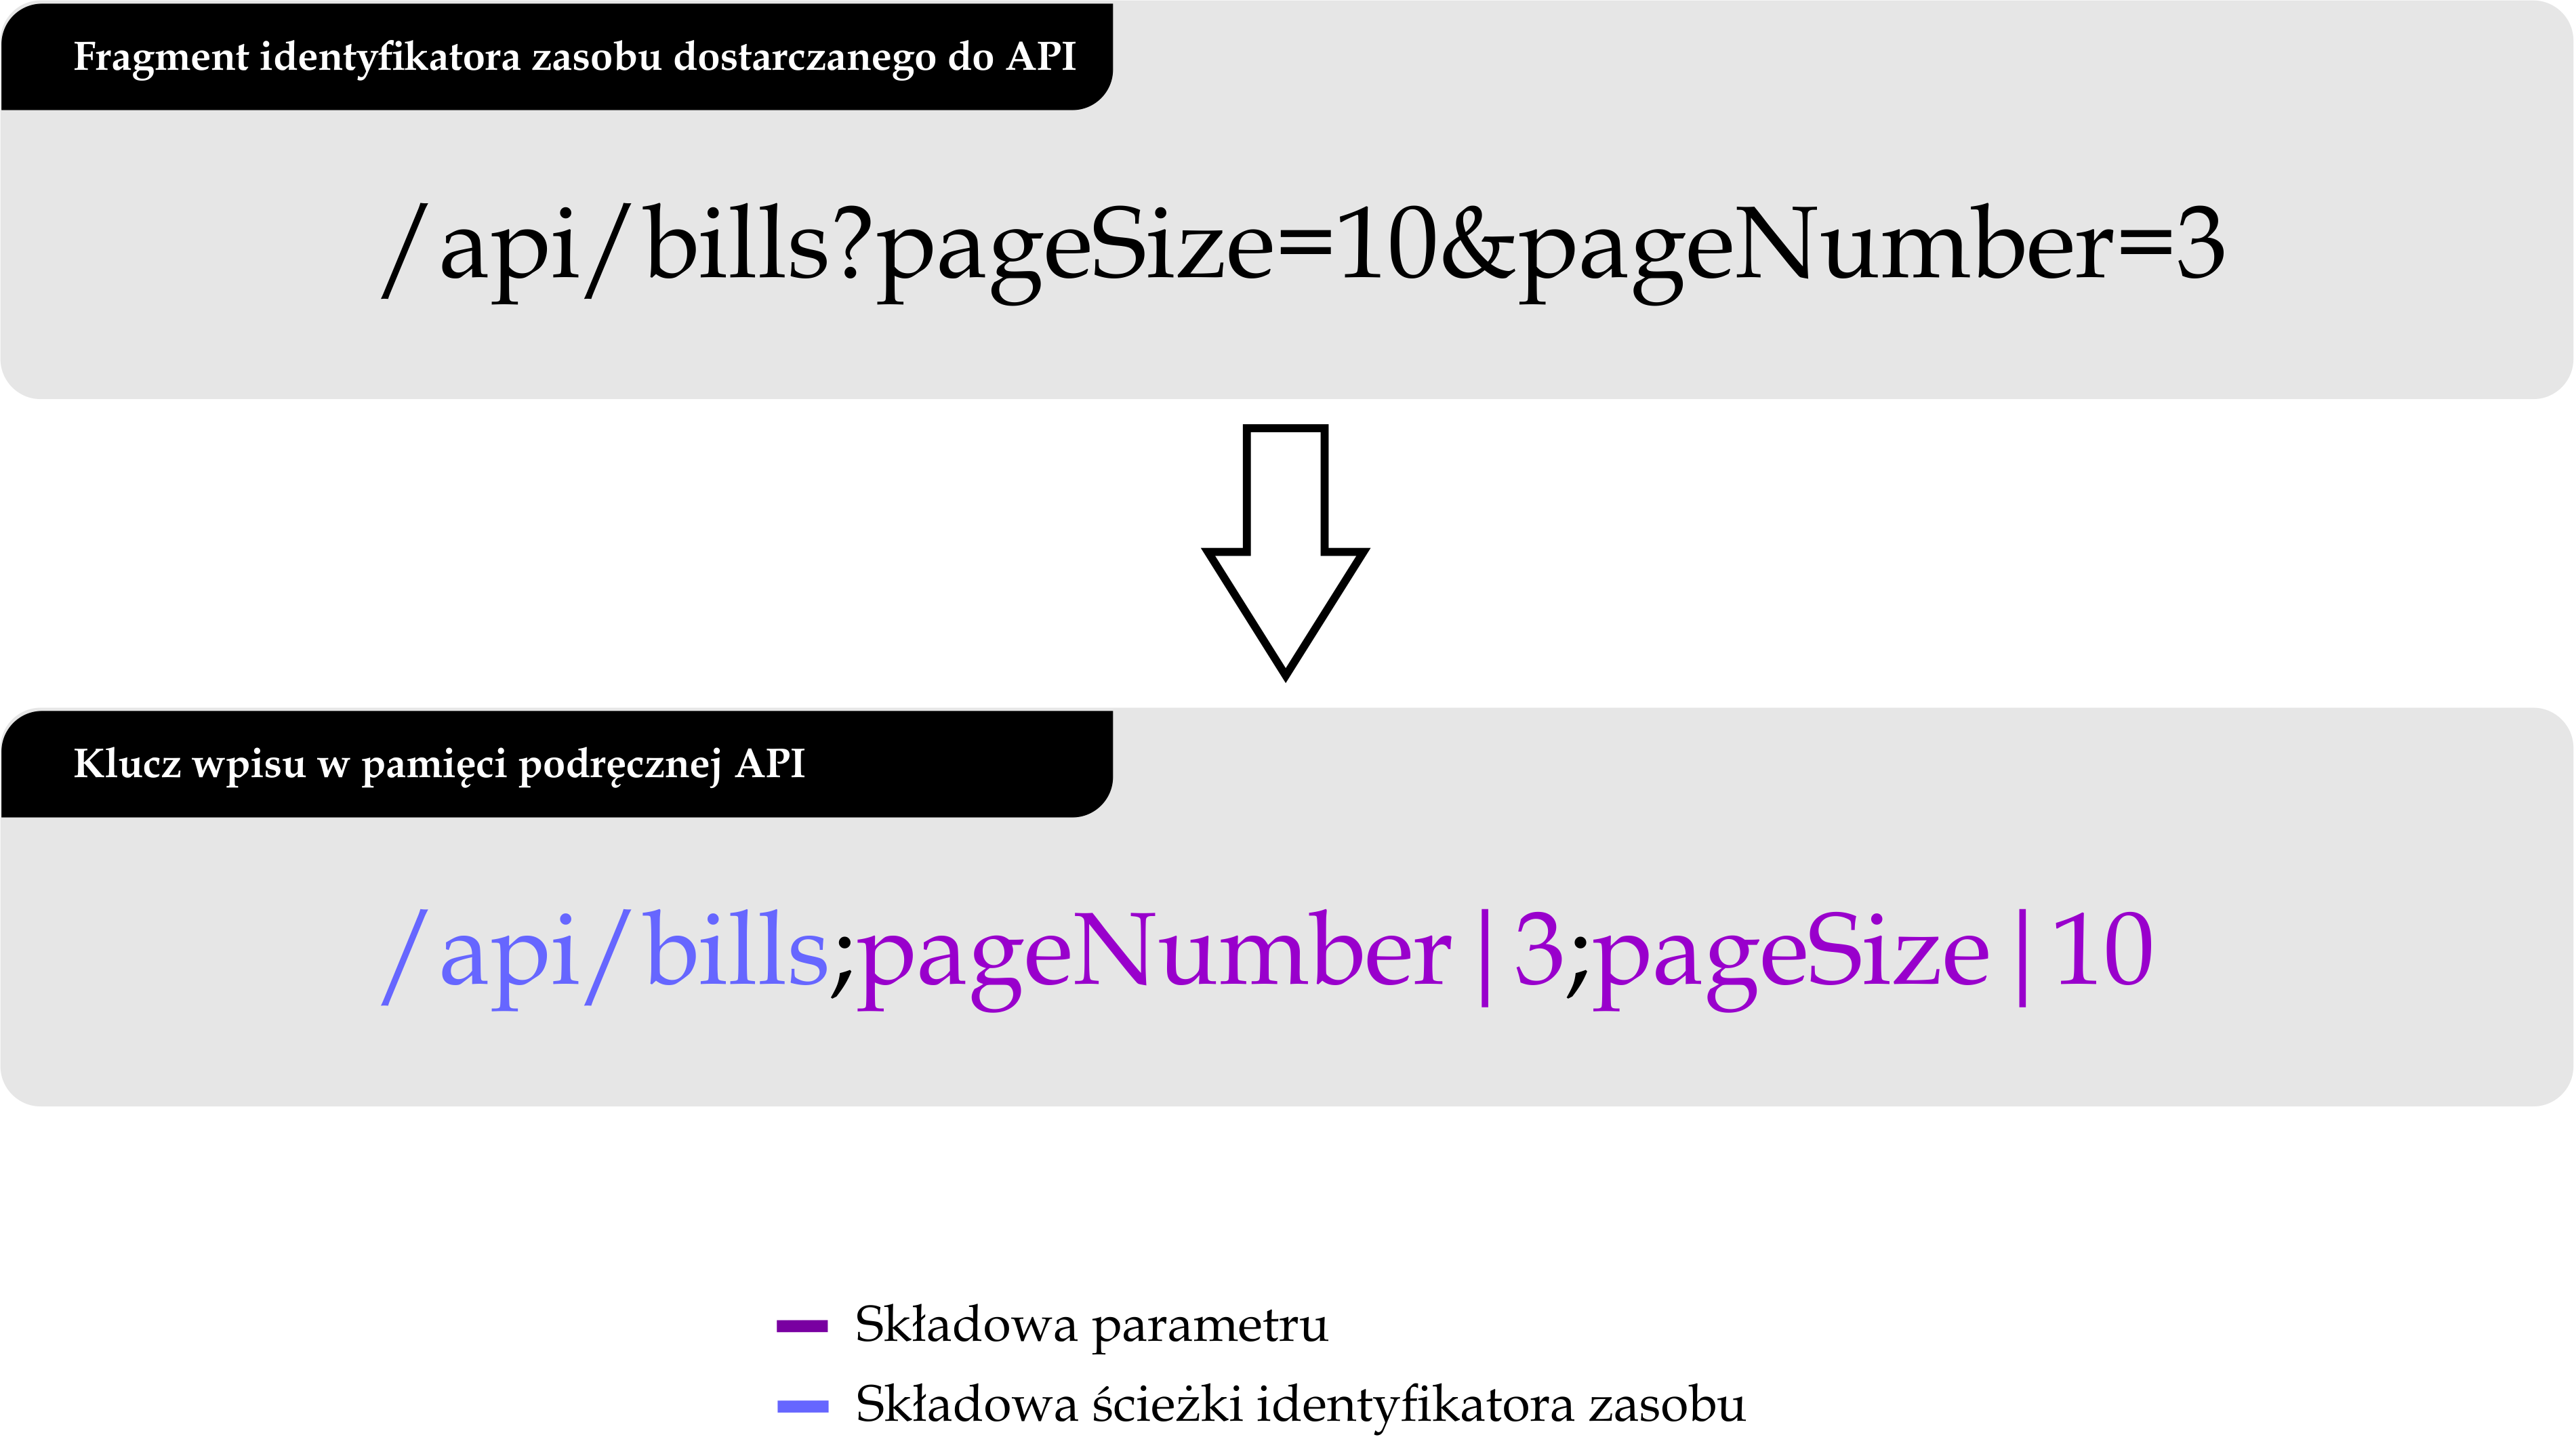
\includegraphics[width=0.8\linewidth]{rys04/cache-klucz.png}
    \caption{Format klucza wpisu przechowywanego w pamięci podręcznej}
    \label{fig:cache-klucz}
\end{figure}

Wdrożone zostały dwa rodzaje mechanizmów obsługi pamięci podręcznej. Pierwszy z nich, zakłada stały czas przechowywania wpisu w magazynie, a także unieważnienie elementu w momencie wywołania metody aktualizacji danych powiązanych z encją opisującą określony element. Mechanizm ten, stanowi klasyczną implementację pamięci podręcznej stosowaną w większości produkcyjnych interfejsów programowania aplikacji.

Drugi mechanizm natomiast, stanowi autorskie podejście twórcy pracy do zarządzania wpisami pamięci podręcznej poprzez ustalenie zmiennego czasu przechowywania elementu w zależności od częstości wywołania punktu końcowego, a także liczby unieważnień. W podejściu tym, wyróżnić należy niezależną strukturę danych, przechowującą liczbę wykonań dla określonego endpointu, a także liczbę wykonań tych punktów końcowych, których działanie prowadzi do unieważnienia wpisu. Przedstawiona struktura jest aktualizowana przy każdym żądaniu wygenerowanym przez klienta i wraz z postępującym działaniem interfejsu programowania aplikacji zawiera coraz bardziej dokładną charakterystykę wywołań poszczególnych obszarów API. Dane te, przechowywane są wewnątrz pamięci programu interfejsu programowania aplikacji, natomiast autor zostawia dowolność co do ich synchronizacji z zewnętrznym źródłem. Synchronizacja ta może być wykonywana poprzez uruchamianie skryptów cyklicznych zadań (np. \textit{cron}), bądź też w momencie uruchamiania oraz wyłączania API.

W momencie tuż przed stworzeniem wpisu i wysyłaniem go do magazynu pamięci podręcznej, w omawianym podejściu następuje kalkulacja czasu życia generowanego elementu. Na początku, obliczany zostaje współczynnik wykonania będący ilorazem liczby uruchomień rozpatrywanego punktu końcowego oraz maksymalnej liczby uruchomień dowolnego z endpointów. Kolejno, w sposób analogiczny tworzony zostaje współczynnik inwalidacji. W tym przypadku stanowi on iloraz wywołań punktów końcowych unieważniających rozpatrywane żądanie i maksymalnej liczby unieważnień dla dowolnego żądania. Oba współczynniki mogą przyjmować wartości z zakresu od zera do jeden. Czas ważności wpisu pamięci podręcznej stanowi iloczyn maksymalnej wartości czasu życia elementu oraz sumarycznego współczynnika wykonania i inwalidacji. Współczynnik ten, określany jest jako suma połowy wartości współczynnika wykonania, a także połowy odwrotności wartości współczynnika unieważnienia. Wprowadzenie takiej formuły prowadzi do uzyskiwania dłuższych czasów przechowywania wpisów dla żądań często wykonywanych oraz rzadko unieważnianych. Wraz ze spadkiem liczby wywołań punktu końcowego, bądź wzrostem liczby jego unieważnień czas ważności wpisu pamięci podręcznej jest zmniejszany. Tak zdefiniowana koncepcja prowadzić powinna do faworyzowania tych punktów końcowych, z których użytkownicy interfejsów korzystają najczęściej.

\begin{equation}
    exec\_factor(x) =  \frac{executions(x)}{max(executions(x):x=1..n)}
    \label{eq:execution-factor}
\end{equation}

\begin{equation}
    invalid\_factor(x) =  \frac{invalidations(x)}{max(invalidations(x):x=1..n)}
    \label{eq:invalidation-factor}
\end{equation}

\begin{equation}
    ttl(x) = (\frac{1}{2} * exec\_factor(x) + \frac{1}{2} * (1 - invalid\_factor(x))) * max\_ttl
    \label{eq:time-to-live}
\end{equation}



gdzie:\newline\newline



$executions(x)$ - liczba wywołań punktu końcowego, którego wpis w pamięci podręcznej identyfikowany jest kluczem x \newline\newline
$invalidations(x)$ - liczba unieważnień wpisu pamięci podręcznej identyfikowanego kluczem x \newline\newline
$execution\_factor(x)$ - współczynnik częstości wykonania określonego punktu końcowego \newline\newline
$invalidation\_factor(x)$ - współczynnik częstości unieważnień wpisów dotyczących określonego punktu końcowego \newline\newline
$ttl(x)$ - czas ważności wpisu dodawanego do pamięci podręcznej \newline\newline
$max\_ttl(x)$ - maksymalny czas ważności wpisu podręcznej względem którego wyliczany jest faktyczny czas ważności \newline\newline

Kod źródłowy służący do zarządzania elementami pamięci podręcznej zaimplementowany został w API C\# za pomocą funkcji pośredniczących dołączanych do struktur programistycznych w formie atrybutu. Stworzona została klasa dziedzicząca po natywnym typie \textit{Attribute}, a także implementująca interfejs \textit{IAsyncActionFilter}. Implementacja niniejszego interfejsu wymaga zdefiniowania metody \textit{OnActionExecutionAsync}, w ramach której napisano logikę działania obu mechanizmów obsługi cache. Wspomniana metoda, posiada dostęp do kontekstu żądania HTTP przez co możliwe było zarówno wykonanie operacji, tuż przed jak i tuż po uruchomieniu metody klasy konstruktora.

W przypadku platformy uruchomieniowej NodeJS oraz języka JavaScript, wymagane było utworzenie dwóch osobnych funkcji, a także rozdzielenie logiki zarządzania pamięcią podręczną, względem operacji wykonywanych przed oraz po uruchomieniu kontrolera. Interfejs programowania aplikacji tworzony z wykorzystaniem omawianych technologii, a także biblioteki ExpressJS, opiera swoje działanie na ciągu kolejno wywoływanych metod, z których ostatnią jest ta, która wysyła odpowiedź do klienta, korzystając z natywnego obiektu odpowiedzi. Taka zasada działania, wymusiła modyfikację kodu źródłowego metod klas kontrolerów w taki sposób, aby rezultat ich wykonania nie zwracał bezpośrednio odpowiedzi w stronę klienta, a przekazywał ją do kolejnej funkcji pośredniczącej. Stwierdzenie to jednak nie jest sprzeczne z informacją przytoczoną na początku tej sekcji. Chociaż zmieniony musiał zostać fragment kodu źródłowego metody kontrolera, to nie zmienia to faktu niezależności i odrębności logicznych operacji przeprowadzanych przez tę metodę.

Uogólniony przepływ sterowania wewnątrz interfejsów API implementujących pamięć podręczną, w kontekście odczytu danych, a także abstrahując od używanej technologii programistycznej, stanowi następującą sekwencję:

\begin{itemize}
    \item Wywołania żądania protokołu HTTP przez aplikację kliencką
    \item Określenie metody klasy konstruktora obsługującej żądanie o wyspecyfikowanych składowych
    \item Wywołanie metody obsługi wpisu pamięci podręcznej dla operacji odczytu (tj. połączenie się z magazynem cache, sprawdzenie dostępności wpisu)
    \item Wywołanie metody klasy konstruktora w przypadku braku wpisu w magazynie cache
    \item Pominięcie metody klasy konstruktora w przypadku uzyskania wpisu z magazynu
    \item Zwrócenie odpowiedzi z jednego z dwóch źródeł danych
\end{itemize}

W aspekcie zapisu danych natomiast wyróżnić możemy poniższe kroki:

\begin{itemize}
    \item Wywołania żądania protokołu HTTP przez aplikację kliencką
    \item Określenie metody klasy konstruktora obsługującej żądanie o wyspecyfikowanych składowych
    \item Wywołanie metody klasy konstruktora
    \item Ustalenie kolekcji kluczy wszystkich wpisów pamięci podręcznej powiązanych z modyfikowaną encją
    \item Unieważnienie wszystkich wpisów na podstawie kluczy uzyskanej kolekcji
    \item Zwrócenie odpowiedzi w kierunku aplikacji klienckiej
\end{itemize}

Obie powyższe sekwencje, w przypadku metody autorskiej wzbogacone zostały o aktualizację informacji o wykonaniu i unieważnieniu punktu końcowego, a także proces wyliczenia współczynników wykonania i unieważnienia. 
\subsection*{Implementacja wzorca projektowego CQRS z uwzględnieniem replikacji pomiędzy źródłami danych}
\label{sec:implementacja-cqrs-i-replikacji}
Implementacja wzorca projektowego podziału odpowiedzialności uwzględnia separację obsługi żądań dotyczących pozyskiwania danych (zwanych zapytaniami), a także żądań manipulacji danymi (zwanych komendami). W kontekście przeprowadzonego badania, niezależnie od omawianej technologii, wewnątrz każdego z interfejsów programowania aplikacji zdefiniowano dwa osobne zbiory encji pełniące role modeli danych. Każdy z modeli bazodanowych, odwołuje się do innego źródła danych, przez co wyróżnić możemy dwa zupełnie odseparowane środowiska zapisu oraz odczytu informacji.

Aby zachować zgodność danych pomiędzy modelami, a co za tym idzie, strukturami bazodanowymi które są odwzorowywane na podstawie tych modeli, skonfigurowano mechanizm replikacji transakcyjnej. W mechaniźmie tym, wyróżnić możemy pojęcia strony publikującej (\textit{ang. Publisher}), dystrybutora transakcji  (\textit{ang. Distributor}), a także subskrybenta (\textit{ang. Subscriber}). Każde z tych pojęć tyczy się określonego systemu bazodanowego i określa jego rolę w procesie replikacji. Jeżeli replikacja wykonywana jest pomiędzy dwoma źródłami bazodanowymi (tj. tak jak w niniejszym przypadku), rola dystrybutora przypisana może być do dowolnego z systemów bazodanowych i determinuje ona sposób generowania komunikatów replikacji. W kontekście omawianego rozwiązania, stroną publikującą i jednocześnie dystrybutorem był serwer bazodanowy wykorzystywany do operacji zapisu. W momencie wykonania zapytania modyfikującego dane w obrębie replikowanego systemu bazodanowego, zapytanie to jest wykonywane lokalnie, a następnie dokonane zmiany są transferowane do bazy danych subskrybenta (w tym przypadku bazy danych obsługującej operacje odczytu). Wprowadzenie takiego mechanizmu pozwoliło na dokonanie całkowitej separacji źródła danych przeznaczonego do zapisu danych, od tego, desygnowanego do ich odczytu.

Na ilustracji \ref{fig:jak-dziala-replikacja} zobrazowano zasadę działania zaimplementowanego mechanizmu replikacji transakcyjnej.

\begin{figure}[ht]
    \centering
     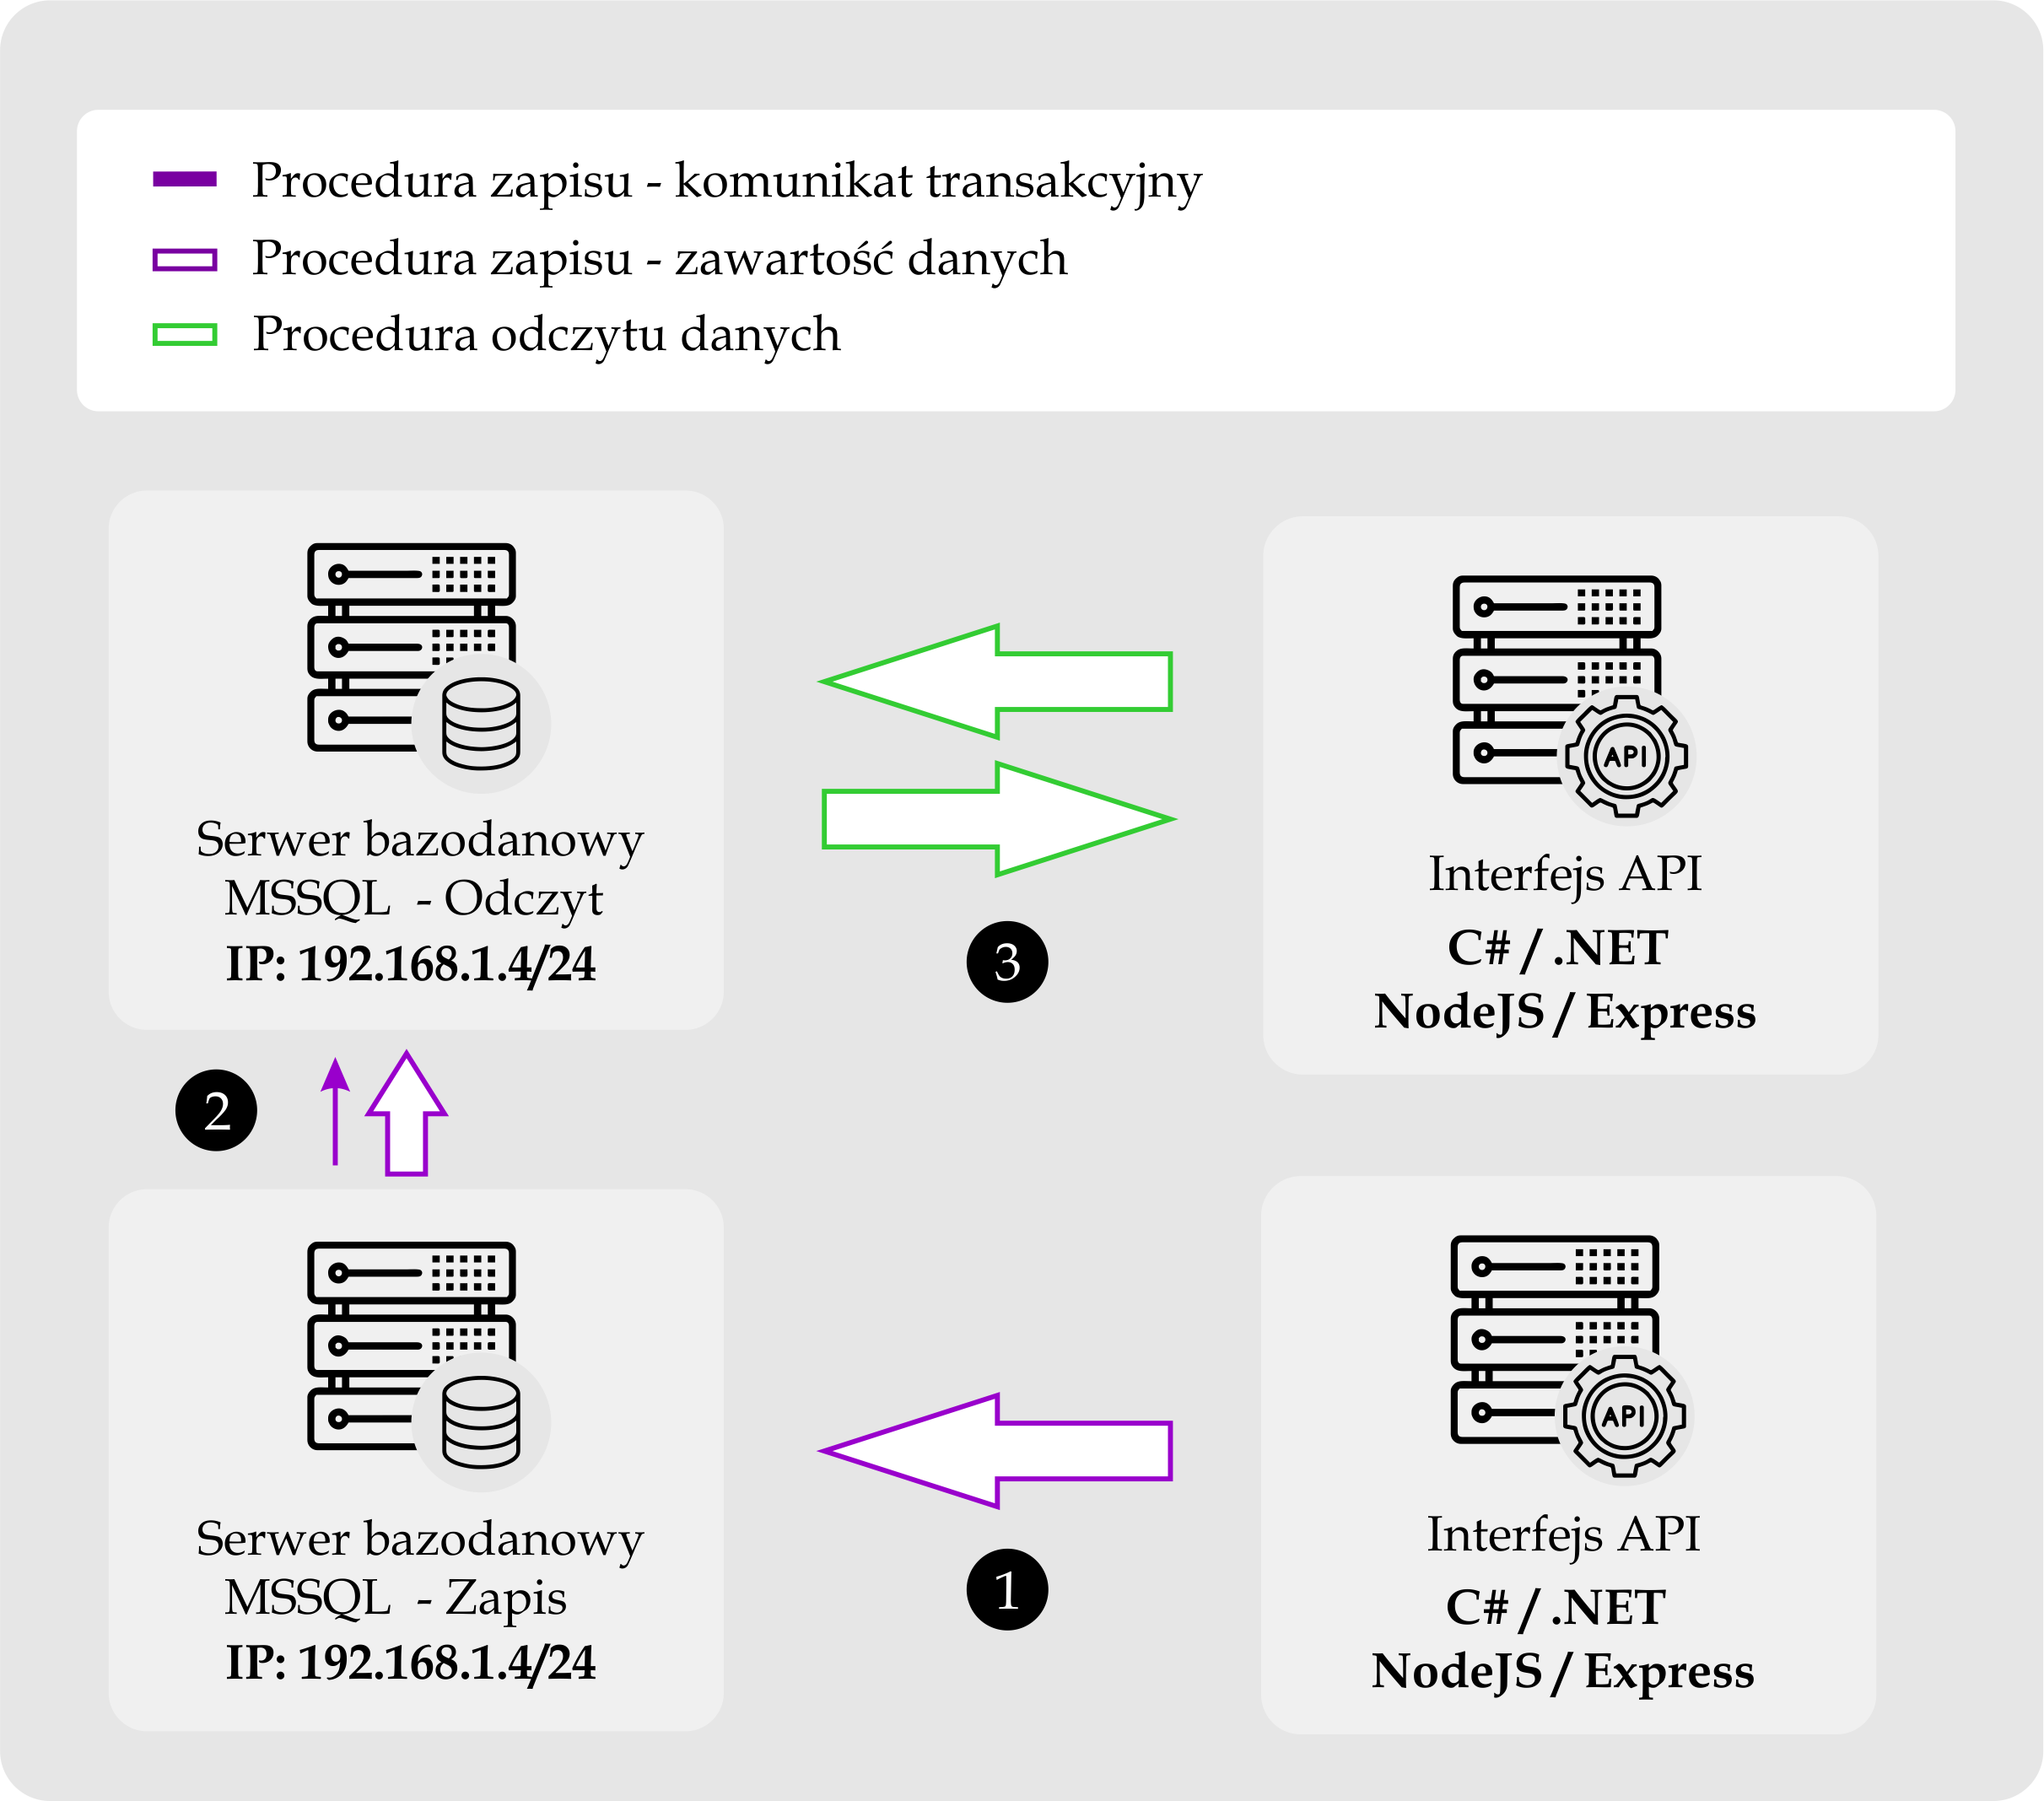
\includegraphics[width=0.6\linewidth]{rys04/jak_dziala_transakcja.png}
    \caption{Schemat wykonywania procedur zapisu oraz odczytu z wykorzystaniem replikacji transakcyjnej}
    \label{fig:jak-dziala-replikacja}
\end{figure}

Zastosowanie omówionego mechanizmu pozwoliło na dokonanie implementacji interfejsów programowania aplikacji, które mogą zarówno uwzględniać dwa odrębne, zoptymalizowane względem typu operacji modele danych, jak i manipulować danymi bez ryzyka wystąpienia nadmiernego opóźnienia wynikającego z konieczności wykonania synchronizacji na poziomie API.   

Podstawową intencją dokonania separacji środowisk zapisu i odczytu, a także wykorzystania wzorca projektowego podziału odpowiedzialności jest możliwość wdrożenia optymalizacji modelu odczytu danych. Optymalizacje te, zarówno dotyczące struktur bazodanowych, jak i rozwiązań programistycznych, mają na celu przyspieszenie procedury odwoływania się, pozyskiwania oraz zwracania danych bezpośrednio do aplikacji klienckiej.  

Zależnie od wykorzystywanej technologii, możliwe było wprowadzenie różnych rozwiązań optymalizacyjnych dotyczących zarówno struktur bazodanowych, jak i generowania zapytań w kierunku bazy danych.

W ramach interfejsu programowania aplikacji uruchamianego w środowisku .NET/C\# wprowadzono następujące usprawnienia wydajnościowe:
\begin{itemize}
    \item Kompilowane kwerendy \textit{(ang. Compiled Queries)} - zapytania o dane linq, wykorzystywane przez mapper entity framework core stanowią intuicyjny i prosty w budowie interfejs komunikacji z systemem bazodanowym. Programista, w nieskomplikowany sposób może zbudować zaawansowaną kwerendę pozyskującą dane, odwołującą się jednocześnie do wielu struktur bazodanowych. Rozwiązanie to jednak, wymaga zbudowania przez bibliotekę entity framework core drzewa składniowego reprezentującego kwerendę i pozwalającego na jej przekształcenie do kodu języka bazy danych. Proces ten, wraz ze zwiększeniem się poziomu skomplikowania zapytania może trwać znacząco dłużej i wpływać negatywnie na wydajność aplikacji. Dlatego też, zastosowano się na wykorzystanie podejścia kompilowanych kwerend, które pozwala na zbudowanie drzew składniowych dla zapytań jednokrotnie po uruchomieniu api, a następnie szybsze generowanie kodu języka bazy danych.
    \item Pula kontekstów bazodanowych \textit{(ang. DbContext Pool)} - dla standardowej konfiguracji interfejsów API w ramach platformy .NET, instancja klasy kontekstu bazodanowego inicjalizowana każdorazowo dla pojedynczego żądania wysyłanego w kierunku API. Rozwiązanie to jest akceptowalne przy standardowym natężeniu otrzymywanych żądań ze względu na niewielki rozmiar instancji klasy, a także szybki czas jej ustanowienia. W przypadku zwiększonego natężenia ruchu sieciowego w kierunku API, wydajność może zostać z tego powodu obniżona. W celu zapobiegania spadku wydajności zastosowano mechanizm puli obiektów kontekstu bazodanowego. Mechanizm ten pozwala na utrzymywanie wielu obiektów konktekstu przez cały czas działania API i czasowe przydzielanie tych obiektów do obsługi nadchodzących żądań.
    \item Leniwe ładowanie \textit{(ang. Lazy loading)} - domyślnym zachowaniem obiektu kontekstu bazodanowego jest wykonanie kwerendy tuż po jej deklaracji, a także pozyskanie wszelkich obiektów nawigacyjnych, które zostały w niej wymienione. Zachowanie to, powoduje pozyskanie określonych fragmentów danych, które zostaną wykorzystane dopiero w dalszej części przetwarzania programu. Mechanizm leniwego ładowania pozwala na pozyskiwanie danych dopiero wtedy, gdy instrukcje kodu źródłowego wskazują na konieczność ich wykorzystania.
    \item Rozdzielone zapytania \textit{(ang. Split Queries)} - kod języka bazy danych, wygenerowany poprzez przetworzenie drzewa składniowego zapytania linq przez entity framework core, domyślnie uwzględnia pozyskiwanie encji zależnych (tj. encji identyfikowanych kluczem obcym) poprzez dokonanie lewostronnego iloczynu kartezjańskiego. Dzięki temu, niezależnie od tego, ile encji zależnych programista będzie chciał uzyskać, operacja pozyskiwania danych sprowadzona zostanie do pojedynczego zapytania. Wiąże się to jednak z możliwością uzyskania bardzo dużej liczby zduplikowanych danych. Dane te, są programowo filtrowane przez maper obiektowo-relacyjny przed zwróceniem ich do kodu programu. Aby uniknąć konieczności redukcji zduplikowanych danych, przy założeniu wykonywania kwerend dołączających wiele encji zależnych wykorzystany został mechanizm rozdzielonych zapytań, który przekształca pojedyncze zapytanie z wielokrotnym lewostronnym iloczynem w serię kilku osobnych zapytań.
    \item Pula połączeń bazodanowych \textit{(ang. Database Connections Pool)} - zdefiniowanie parametru obsługi wielu równolegle działających połączeń z serwerem bazodanowym. 
\end{itemize}

Ponadto, wprowadzono wiele mniej znaczących usprawnień wydajnościowych, takich jak przekazywanie parametrów do zapytań linq zamiast stosowania stałych dosłownych, czy też redukcja wykorzystania zewnętrznych metod wewnątrz funkcji anonimowych zapytania. 

W ramach interfejsu programowania aplikacji uruchamianego w środowisku NodeJS/Express wprowadzono następujące usprawnienia wydajnościowe:
\begin{itemize}
    \item Wykorzystanie obiektu include do dołączania encji zależnych w sposób kontrolowany przez mapper obiektowo-relacyjny prisma, tak aby zredukować możliwość wystąpienia problemu n+1 zapytań.
    \item Zdefiniowanie pojedynczej, globalnej instancji klienta mappera obiektowo-relacyjnego \textit{PrismaClient}, w celu redukcji konieczności każdorazowego dokonywania operacji zajęcia i zwolnienia pamięci, a także czasu potrzebnego na nawiązanie połączenia pomiędzy klientem a instancją systemu bazodanowego.
    \item Pula połączeń bazodanowych - zdefiniowanie parametru obsługi wielu równolegle działających połączeń z serwerem bazodanowym. 
\end{itemize}

Co więcej, wprowadzono również następujące optymalizacje wydajności ściśle dotyczące struktur bazodanowych:
\begin{itemize}
    \item Zdefiniowanie indeksów oraz określenie pól jako unikalne w celu przyspieszenia procesu odwoływania się do danych, a także ich filtracji oraz sortowania
    \item Ograniczenie przedziałów liczbowych dla pól numerycznych oraz maksymalnych długości dla ciągów tekstowych
    \item Przekształcenie określonych pól ciągów tekstowych z typu \textit{NVARCHAR} wykorzystującego do kodowania pojedynczego znaku 2 bajty (kodowanie UTF16), do typu \textit{VARCHAR} wykorzystującego do kodowania pojedynczego znaku jeden bajt.
\end{itemize}
\section{Konfiguracja generycznych oraz dedykowanych platform chmurowych}
W kontekście przeprowadzanych ewaluacji skonfigurowano trzy platformy chmurowe, w ramach których uruchomiono badane interfejsy programowania aplikacji. Wykorzystanie odmiennych platform chmurowych jako środowisk wdrożeniowych dla interfejsów API ma na celu dokonanie obserwacji zmiany wydajności działania systemów internetowych względem poziomu przystosowania usługi wdrożeniowej w odniesieniu do konkretnego interfejsu programowania aplikacji. Oznacza to, że ewaluowane zostały zarówno rozwiązania o wysokim stopniu ogólności (tj. dostarczające możliwości pełnego zarządzania systemem operacyjnym serwera, na którym wdrożone zostały aplikacje), jak i te, które bezpośrednio powiązane są z określoną technologią implementacyjną.

W ramach pierwszej z omawianych platform chmurowych, wykorzystano usługę typu \textit{Infrastructure as a Service} w postaci wirtualnego serwera prywatnego udostępnionego przez dostawcę usług chmurowych \textit{DigitalOcean}. Serwer ten, posiadał 25GB pamięci dyskowej, 16GB pamięci operacyjnej o dostępie swobodnym, a także ośmiordzeniową centralną jednostkę przetwarzania o architekturze 64-bitowej. Na omawianym serwerze zainstalowano dystrybucję systemu operacyjnego Linux o nazwie \textit{Ubuntu Server} w wersji 22.04 LTS.

Niezależnie od technologii wdrażanego interfejsu programowania aplikacji, zdecydowano się na wykorzystanie tego samego serwera usługi WWW, którym w tym przypadku było oprogramowanie \textit{Apache2}. Usługa ta, pełniła rolę odwróconego serwera pośredniczącego \textit{(ang. Reverse-proxy)}, pomiędzy serwerem interfejsu API a zlokalizowanymi na zewnątrz sieci urządzeniami klienckimi. Serwerem interfejsu API napisanego w języku C\# było oprogramowanie \textit{Kestrel}, natomiast w przypadku NodeJS API, usługą wykorzystywaną do hostowania aplikacji w środowisku lokalnym był framework \textit{ExpressJS}. Oba, spośród wymienionych serwerów aplikacji uruchomione były w obrębie systemu operacyjnego w postaci programów typu demon działających w tle. Oprogramowanie poszczególnych interfejsów programowania aplikacji uruchomione było tylko na czas przeprowadzania ewaluacji i nigdy nie funkcjonowało w sposób równoległy.

Drugi z zastosowanych mechanizmów wdrożeniowych to rozwiązanie typu \textit{Platform as as Service} udostępniane przez dostawcę usług chmurowych \textit{Microsoft Azure}. W tym przypadku, programista zarządzać może uruchomionymi usługami, określać konfigurację każdej z nich, natomiast nie posiada on dostępu do warstw uruchamiania programów, czy też administrowania systemem operacyjnym. Aby zapobiec niereprezentatywności wyników badań przeprowadzanych w obrębie przedstawianego środowiska chmurowego, zdecydowano się na skorzystanie z opcji dynamicznego przydziału zasobów sprzętowych do skonfigurowanych usług, z zastrzeżeniem maksymalnych wartości pojemności dyskowej do 25GB, pamięci RAM do 16GB, a także liczby wykorzystywanych rdzeni centralnej jednostki przetwarzania do ośmiu. Na omawianej platformie uruchomiono usługę interfejsu programowania aplikacji napisanego w języku C\# z wykorzystaniem platformy .NET, a także system bazodanowy Microsoft SQL Server.

Odnosząc się do ostatniej spośród eksploatowanych platform chmurowych, zastosowano rozwiązanie typu \textit{Platform as a Service} dostawcy usług \textit{Heroku}. Rozwiązanie to, jest rekomendowanym sposobem wdrożenia aplikacji internetowych opartych o środowisko NodeJS. Analogicznie do platformy udostępnianej przez dostawcę DigitalOcean, w przypadku usługi Heroku istnieje możliwość doboru komponentów sprzętowych dostępnych w ramach fizycznej maszyny hostującej. W związku z tym faktem, a także w celu zapobiegania uprzywilejowaniu któregokolwiek z rozwiązań w kontekście przeprowadzanych badań, zastosowano te same wartości pojemności dyskowej, pojemności pamięci operacyjnej, a także liczby rdzeni procesora. Dostęp do systemu operacyjnego urządzenia serwerowego, zgodnie z typem przedstawianej usługi, nie jest przyznany użytkownikowi. Na omawianej platformie uruchomiono usługę interfejsu programowania aplikacji napisanego w języku JavaScript z wykorzystaniem platformy NodeJS/Express, a także nierelacyjny system bazodanowy MongoDB.
\section{Konfiguracja narzędzia do realizacji badań}
Narzędziem wykorzystanym do przeprowadzenia procesu ewaluacji wydajności interfejsów programowania aplikacji było otwartoźródłowe oprogramowanie Apache JMeter. Przytoczone rozwiązanie informatyczne dostarcza możliwości definiowania, konfiguracji, a także wykonywania testów wydajności usług sieciowych, z uwzględnieniem zmiennego natężenia ruchu sieciowego, kontrolowanego przez użytkownika. Jedną z kluczowych zalet omawianego narzędzia jest możliwość kompozycji testów wydajnościowych o charakterze rozproszonym. Możliwość ta, została wykorzystana w ramach przeprowadzonych badań, dzięki czemu w czasie pojedynczej ewaluacji, żądania generowane były ze zmiennej liczby urządzeń klienckich.

Pierwszym etapem konfiguracji oprogramowania JMeter było przystosowanie wszystkich instancji tego narzędzia, ulokowanych w obrębie poszczególnych hostów sieci komputerowej. Przystosowanie to, sprowadzało się do edycji plików właściwości programu, a także skryptu programowania wsadowego uruchamiającego plik wykonywalny JMeter. Niezbędnym krokiem w kierunku ustanowienia komunikacji pomiędzy hostami było również wyłączenie systemowej usługi zapory sieciowej.

Implementacja ustawień programu JMeter dla komputera pełniącego rolę koordynatora testów sprowadzała się do modyfikacji zawartości pliku \textit{jmeter.properties}. W pliku tym, wyszczególniono adresy internetowe hostów typu slave, przypisano numer portu dla serwera zdalnego wywoływania metod, wskazano lokalizację pliku przechowującego klucz szyfrowania komunikacji, a także ustawiono opcję wykorzystania protokołu SSL do komunikacji za pomocą usługi RMI. Pozostała zawartość pliku nie uległa zmianie. Na listingu \ref{list:jmeter-properties} pokazano fragment omawianego pliku właściwości zawierający zmodyfikowane wpisy.

\begin{lstlisting}[ label=list:jmeter-properties, caption=Modyfikowane właściwości pliku konfiguracyjnego JMeter, basicstyle =\footnotesize \ttfamily]
remote_hosts=192.168.1.101, 192.168.1.102
server.rmi.port=1099
server.rmi.keystore.type=JKS
server.rmi.keystore.file=ssl_master_thesis_testing.jks
server.rmi.keystore.password=master_thesis
server.rmi.ssl.disable=false
\end{lstlisting}

W analogiczny sposób zmodyfikowano zawartość plików konfiguracyjnych dla każdej z maszyn pełniących role generatorów żądań. W tym przypadku jednak, klucz \textit{remote\_hosts} zawierał tylko i wyłącznie adres IP hosta typu master, a plik klucza prywatnego, uprzednio wygenerowany na maszynie master, został rozdystrybuowany pomiędzy maszynami slave. Po wykonaniu opisanych czynności, na każdym z hostów-generatorów uruchomiono plik wsadowy \textit{jmeter-server}, nasłuchujący poleceń od urządzenia typu master.

Po realizacji czynności związanych z ustanowieniem transmisji pomiędzy maszynami, sporządzono plany testowe dotyczące poszczególnych scenariuszy badawczych. Wyróżnić należy dwa plany testowe, których określone warianty pozwoliły na przeprowadzenie każdej z ewaluacji określonych w ramach scenariuszy badawczych. 

\subsection*{Plan testowy nr. 1}
\label{plan-testowy-1}
Pierwszy z planów testowych, stworzony został w celu obserwacji sposobu działania interfejsów programowania aplikacji względem zwiększającego się poziomu natężenia równolegle generowanego ruchu sieciowego. Podstawowym elementem schematu ewaluacyjnego jest grupa współbieżnie działających wątków \textit{(ang. Concurrency Thread Group)}. W przeciwieństwie do standardowej implmentacji mechanizmu grupy wątków, dostępnej w ramach oprogramowania JMeter, grupa wątków współbieżnych pozwala na kumulowanie liczby aktywnych procesów w czasie testu, pozwalając na ich zakończenie dopiero w momencie określonym przez użytkownika. Moment ten, w kontekście niniejszych testów przypadał na chwilę zakończenia badania. Dzięki zastosowaniu takiego rozwiązania, możliwe było symulowanie zjawiska stopniowego wzrostu natężenia ruchu generowanego równolegle przez określoną liczbę użytkowników. Wybór standardowej grupy wątków, prowadziłby do finalnego uruchomienia określonej liczby procesów, jednakże nie pozwalałby na kontrolę momentu ich zakończenia, co prowadziłoby do zmiennego poziomu natężenia żądań, posiadającego charakterystykę losową, a także niepowiązanego z czasem trwania testu.

Kolejne składowe występujące w ramach planu testowego, podzielić należy na cztery grupy. 

Pierwszą z nich są elementy konfiguracyjne \textit{(ang. Config Elements)}. W elementach tych, określono: adres IP interfejsu programowania aplikacji, port TCP, rodzaj protokołu hipertekstowego, immplementację klienta HTTP (wybrano domyślną - HttpClient4), a także czasy upłynięcia limitu czasu połączenia (30000ms) oraz uzyskania odpowiedzi (120000ms).

Kolejna z grup składowych zawiera próbniki \textit{(ang. Samplers)}. Elementy te, dostarczają informacji o punktach końcowych API, do których wysyłane mają być żądania. Do każdego z próbników, dołączyć można indywidualny element konfiguracyjny, a także mechanizm weryfikacji poprawności realizacji żądania nazywany asercją \textit{(ang. Assertions)}. W przypadku niniejszego planu testowego, wprowadzono asercje dotyczące kodu odpowiedzi HTTP, a także jej schematu w postaci notacji JSON.

Ostatnie spośród zawartych składowych to nasłuchiwacze \textit{(ang. Listeners)}. Posiadają one postaci raportów, tabel, a także wizualizacji dotyczących przeprowadzonego testu.

Na ilustracji \ref{fig:test-plan-1} przedstawiono zastosowane elementy składowe pierwszego planu testowego.

\begin{figure}[ht]
    \centering
     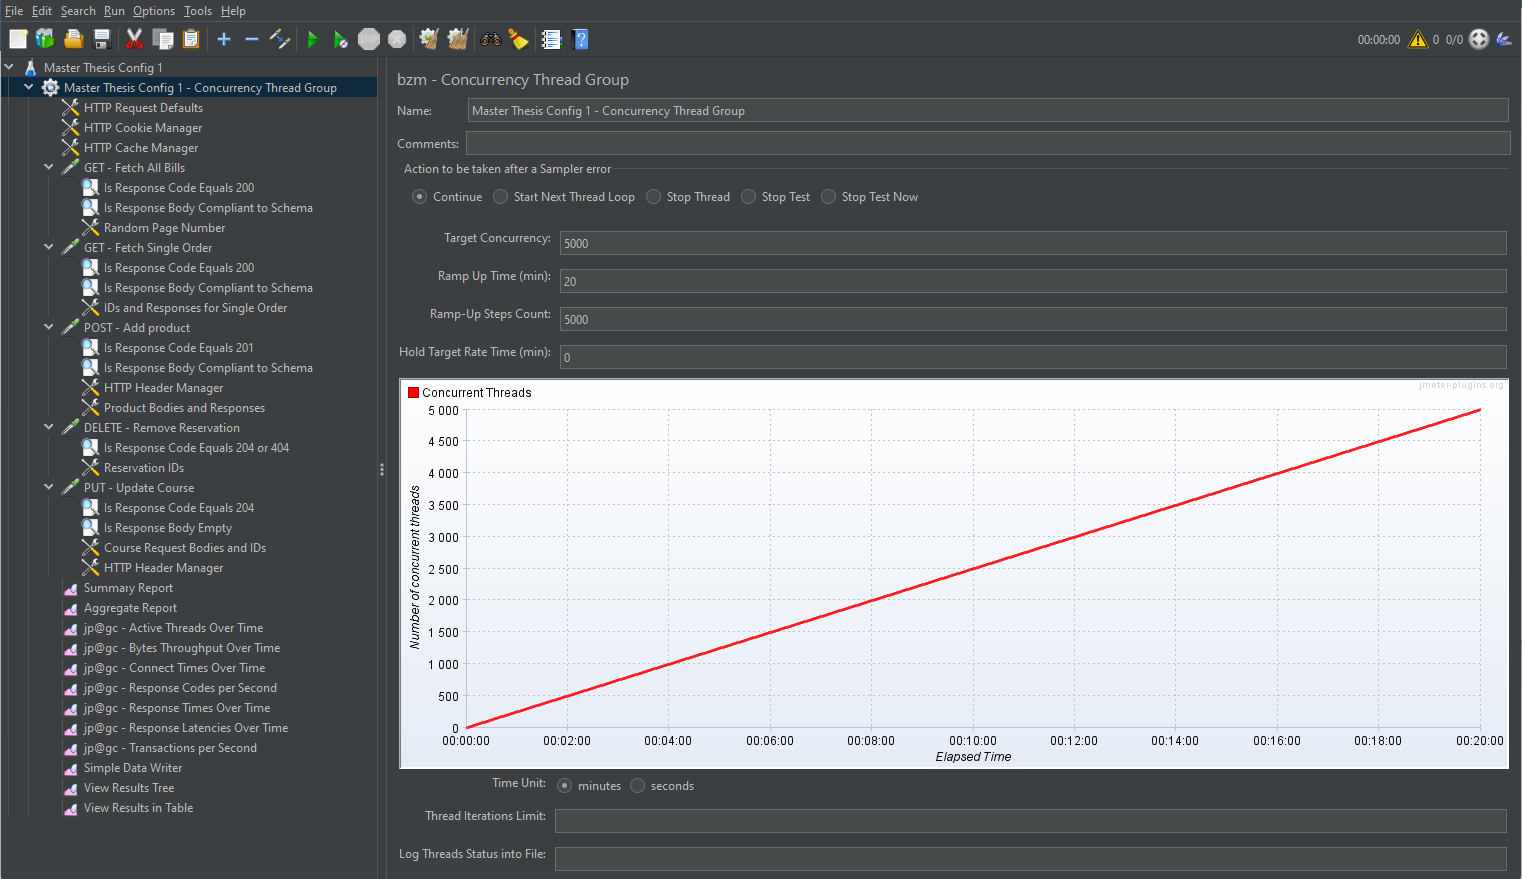
\includegraphics[width=\linewidth]{rys04/test-plan-1.png}
    \caption{Konfiguracja pierwsza planu testowego JMeter}
    \label{fig:test-plan-1}
\end{figure}

\subsection*{Plan testowy nr. 2}
\label{plan-testowy-2}
Drugi z planów testowych, został przygotowany w kontekście wywoływania punktów końcowych o stałym czasie odpowiedzi, realizujących operacje charakteryzujące się wysokim kosztem obliczeniowym. W tym przypadku, zdefiniowano współbieżną grupę wątków o stałej liczebności równej 100. Czas podtrzymania każdego ze stu procesów określony został na 68000 sekund, co wynikało z założenia najbardziej pesymistycznego scenariusza badań, wykorzystujących ten właśnie plan. Ponadto, wprowadzono elementy konifguracyjne dotyczące komunikacji z API z wykorzystaniem protokołu internetowego, a także, analogiczne względem pierwszego planu komponenty nasłuchujące. Spośród składowych próbników, wymienić należy dwa moduły dotyczące wywołania punktów końcowych interfejsów programowania aplikacji dla porównywanych technologii. Każdy z modułów zawierał asercje dotyczące występowania określonych właściwości w ramach odpowiedzi JSON, a także zbiory danych pomocniczych oraz element konfiguracyjny nagłówka żądania.  

Na ilustracji \ref{fig:test-plan-2} przedstawiono zastosowane elementy składowe drugiego planu testowego.

\begin{figure}[ht]
    \centering
     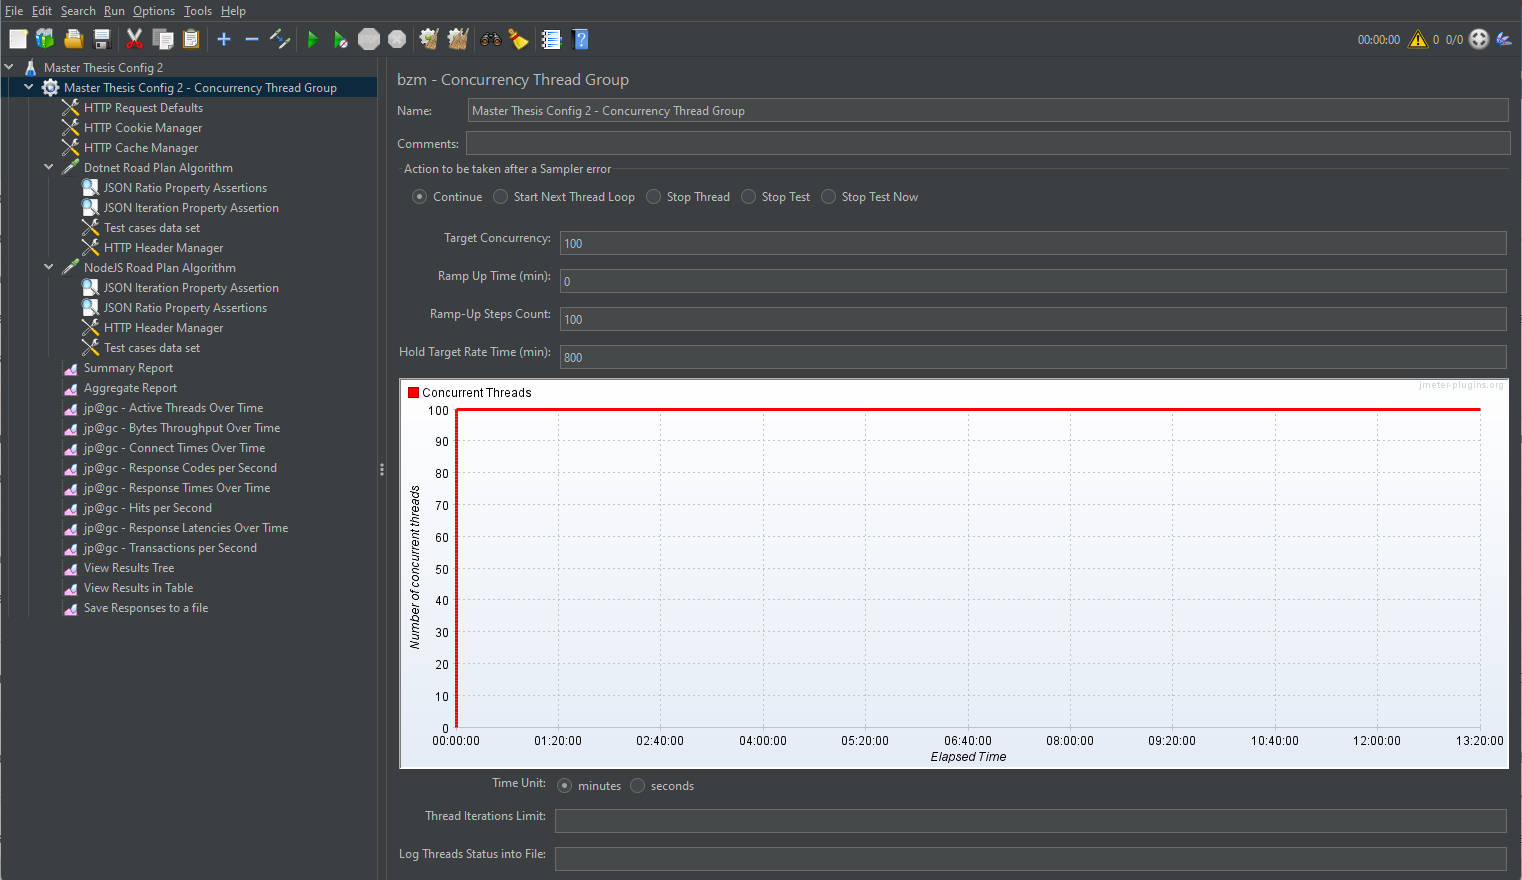
\includegraphics[width=\linewidth]{rys04/test-plan-2.png}
    \caption{Konfiguracja druga planu testowego JMeter}
    \label{fig:test-plan-2}
\end{figure}

\subsection*{Plan testowy nr. 2 - wariant 1}
\label{plan-testowy-2-wariant-1}
Wariant pierwszy drugiego planu testowego wykorzystany został w kontekście obsługi punktów końcowych realizujących operacje asynchroniczne, poprzez odwołania do zewnętrznej usługi. Wprowadzone modyfikacje względem drugiego planu testowego obejmują zastosowanie innych elementów próbników (w tym przypadku elementów odwołujących się do punktów końcowych ewaluacji operacji asynchronicznych), a także wprowadzenie alternatywnej wartości czasu wykonania testu wynoszącej dziesięć minut

\subsection*{Plan testowy nr. 2 - wariant 2}
\label{plan-testowy-2-wariant-2}
Drugi z wariantów planu testowego dostosowano względem ewaluacji wydajności mechanizmów pamięci podręcznej. Liczba wątków w obrębie grupy ograniczona została do trzydziestu, a czas przeprowadzenia badania ustanowiono na 20 minut. Ponadto, wprowadzono komponenty próbników specyficzne w odniesieniu do badania mechanizmów cache. Należy także wspomnieć o wprowadzeniu próbnika pełniącego rolę mechanizmu unieważnienia wpisów pamięci podręcznej. Próbnik ten, wywoływany był tylko i wyłącznie w określonych momentach testu. Takie zachowanie, osiągnięto poprzez wprowadzenie elementu kontrolera przepływności \textit{(ang. Throughput Controller)}, determinującego liczbę wywołań próbnika, a także licznika czasu \textit{(ang. Constant Timer)}, wskazującego na moment wywołania. 
\chapter{Przeprowadzone badania}
W niniejszym rozdziale przedstawiono oraz omówiono badania przeprowadzone w celu ewaluacji wydajności interfejsów API implementowanych z wykorzystaniem porównywanych technologii. Każde z wykonanych badań oparte jest o scenariusz testowy określony w ramach sekcji \ref{sec:scenariusze-badawcze}, a także dotyczy odmiennych aspektów działania usługi sieciowej interfejsu programowania aplikacji. W kojenych sekcjach tego rozdziału w sposób szczegółowy opisano podjęte czynności badawcze, zwizualizowano rezultaty każdej z ewaluacji, dokonano analizy statystycznej, a także sformułowano wnioski.

\section{Wpływ zastosowanego systemu bazodanowego na efektywność działania interfejsu API}
\label{research:crud}
W ramach badania zobserwowano zmianę wydajności działania interfejsów programowania aplikacji względem skomunikowanego z nim systemu bazodanowego. Wykorzystano cztery najpopularniejsze relacyjne systemy baz danych (tj. MySQL, SQL Sever, PostgreSQL oraz SQlite), a także jeden system nierelacyjny (tj. MongoDB). Interfejsy programowania aplikacji komunikujące się z poszczególnymi systemami bazodanowymi poddawane były coraz to większemu obciążeniu, poprzez zwiększanie liczby procesów generujących żądania.

Pierwszą czynnością wykonaną w ramach ewaluacji było spełnienie warunków początkowych dotyczących podjęcia czynności badawczych. Warunki te, uwzględniały realizację testów funkcjonalnych gwarantujących poprawność działania punktów końcowych interfejsu programowania aplikacji. Ponadto, przeprowadzenie tego rodzaju testów pozwoliło na określenie progów tolerancji oraz frustracji wykorzystywanych w kontekście późniejszego wyliczania wartości wskaźnika wydajności aplikacji APDEX.

Ewaluacja funkcjonalna, polegała na uruchomieniu testu uwzględniającego 30 współbieżnie pracujących wątków oprogramowania JMeter, które wysyłały żądania w kierunku punktów końcowych API w czasie 10 minut.

Poczynione zostały dwa następujące założenia:
\begin{itemize}
    \item generowanie żądań przez 30 współbieżnych procesów jest interpretowane jako funkcjonowanie interfejsu programowania aplikacji w standardowych warunkach pracy.
    \item ogólna ocena wydajności systemu, a także progi uwzględniane w ramach wskaźnika APDEX generowane są na podstawie tylko tych punktów końcowych, które poddawane są ewaluacji.
\end{itemize}

Zdecydowano się na wybór pięciu punktów końcowych obsługujących różne metody protokołu hipertekstowego, po to, aby weryfikować każdy rodzaj działania uwzględnianego w ramach funkcjonalności interfejsu API.

W tabeli \ref{tab:endpointy-scenario-1} wyszczególniono każdy z wykorzystywanych punktów końcowych interfejsów programowania aplikacji, a także opisano sposób jego działania.

\begin{table}[htb]
  \centering
  \caption{Wykaz punktów końcowych wykorzystywanych w badaniu wpływu wykorzystanego systemu bazodanowego na działanie API}
  \label{tab:endpointy-scenario-1}
  \resizebox{\columnwidth}{!}{%
  \begin{tabular}[c]{|l|m{0.4\textwidth}|l|m{0.4\textwidth}|}
  \hline
  Identyfikator zasobu &
    Dostarczana zawartość &
    \begin{tabular}[c]{@{}l@{}}Rodzaj \\ metody HTTP\end{tabular} &
    Opis działania \\ \hline\hline
  /api/bills &
    \begin{tabular}[c]{@{}l@{}}\textbf{pageSize} - rozmiar strony (tj. liczba \\ rekordów) -- ustalony na stałe jako 30 \\ \textbf{pageNumber} - numer strony \\ -- generowany zgodnie z jednostajnym \\ rozkładem prawdopodobieństwa\end{tabular} &
    GET &
    Zwrócenie listy encji identyfikujących rachunki wygenerowane w restauracji. Zarówno rozmiar strony, jak i liczba pomijanych rekordów zadane są jako parametr, a poszczególny element listy, zawiera zarówno dane encji podstawowej, jak i każdej z encji zależnych, powiązanych z nią kluczem obcym. \\ \hline
  /api/orders/:id &
    \textbf{id} - identyfikator zamówienia wskazujący każdorazowo zamówienie istniejące w bazie danych &
    GET &
    Zwrócenie pojedynczej encji identyfikującej określone zamówienie poczynione w ramach pobytu w restauracji. Zwrócony element zawiera zarówno dane encji podstawowej, jak i każdej z encji zależnych, powiązanych z nią kluczem obcym. \\ \hline
  /api/products &
  \textbf{saveProductBody} - zasób zapisany w formacie JSON, dostarczający informacje o wartościach właściwości nowo tworzonego produktu -- każdy z identyfikatorów encji zależnych wskazuje na istniejący obiekt &
    POST &
    Dodanie pojedynczej encji do zbioru danych z poprzedzającą je walidacją danych dostarczonych w ramach ciała żądania. \\ \hline
  /api/courses/:id &
  \begin{tabular}[c]{@{}l@{}} \textbf{id} - identyfikator posiłku zawartego \\ w ramach zamówienia wskazujący \\ każdorazowo istniejącą \\ encję bazodanową \\ updateCourseBody - zasób zapisany \\ w formacie JSON, dostarczający \\ informacje o wartościach właściwości \\ modyfikowanego obiektu posiłku \end{tabular} &
    PUT &
    Modyfikowanie encji bazodanowej dotyczącej posiłku zawartego w ramach zamówienia z uprzednią weryfikacją poprawności danych ciała żądania. \\ \hline
  /api/reservations/:id &
  \textbf{id} - identyfikator rezerwacji, wskazujący na istniejący bądź nieistniejący zasób &
    DELETE &
    Usunięcie pojedynczego obiektu rezerwacji, bądź zwrócenie informacji o jego nie znalezieniu w systemie bazodanowym. \\ \hline
  \end{tabular}%
  }
\end{table}

Na wykresie \ref{fig:wykres-testy-funkcjonalne-dotnet} przedstawiono rzeczywiste pomiary chwilowe czasu odpowiedzi na żądanie, uwzględniające rezultaty otrzymane dla każdego z omówionych punktów końcowych. Jako interfejs programowania aplikacji poddawany ewaluacji zastosowano usługę sieciową implementowaną w technologii C\#/.NET, a także komunikującą się z bazą danych SQL Server.

W ramach ewaluacji funkcjonalnej wszystkie wywołania badanych punktów końcowych zwróciły zarówno poprawny kod odpowiedzi, jak i spodziewaną zawartość. Obserwacja ta, pozwoliła na kontynuację badania oraz spełnienie jego warunków początkowych. 

\clearpage

\begin{figure}[htb]
    \centering
     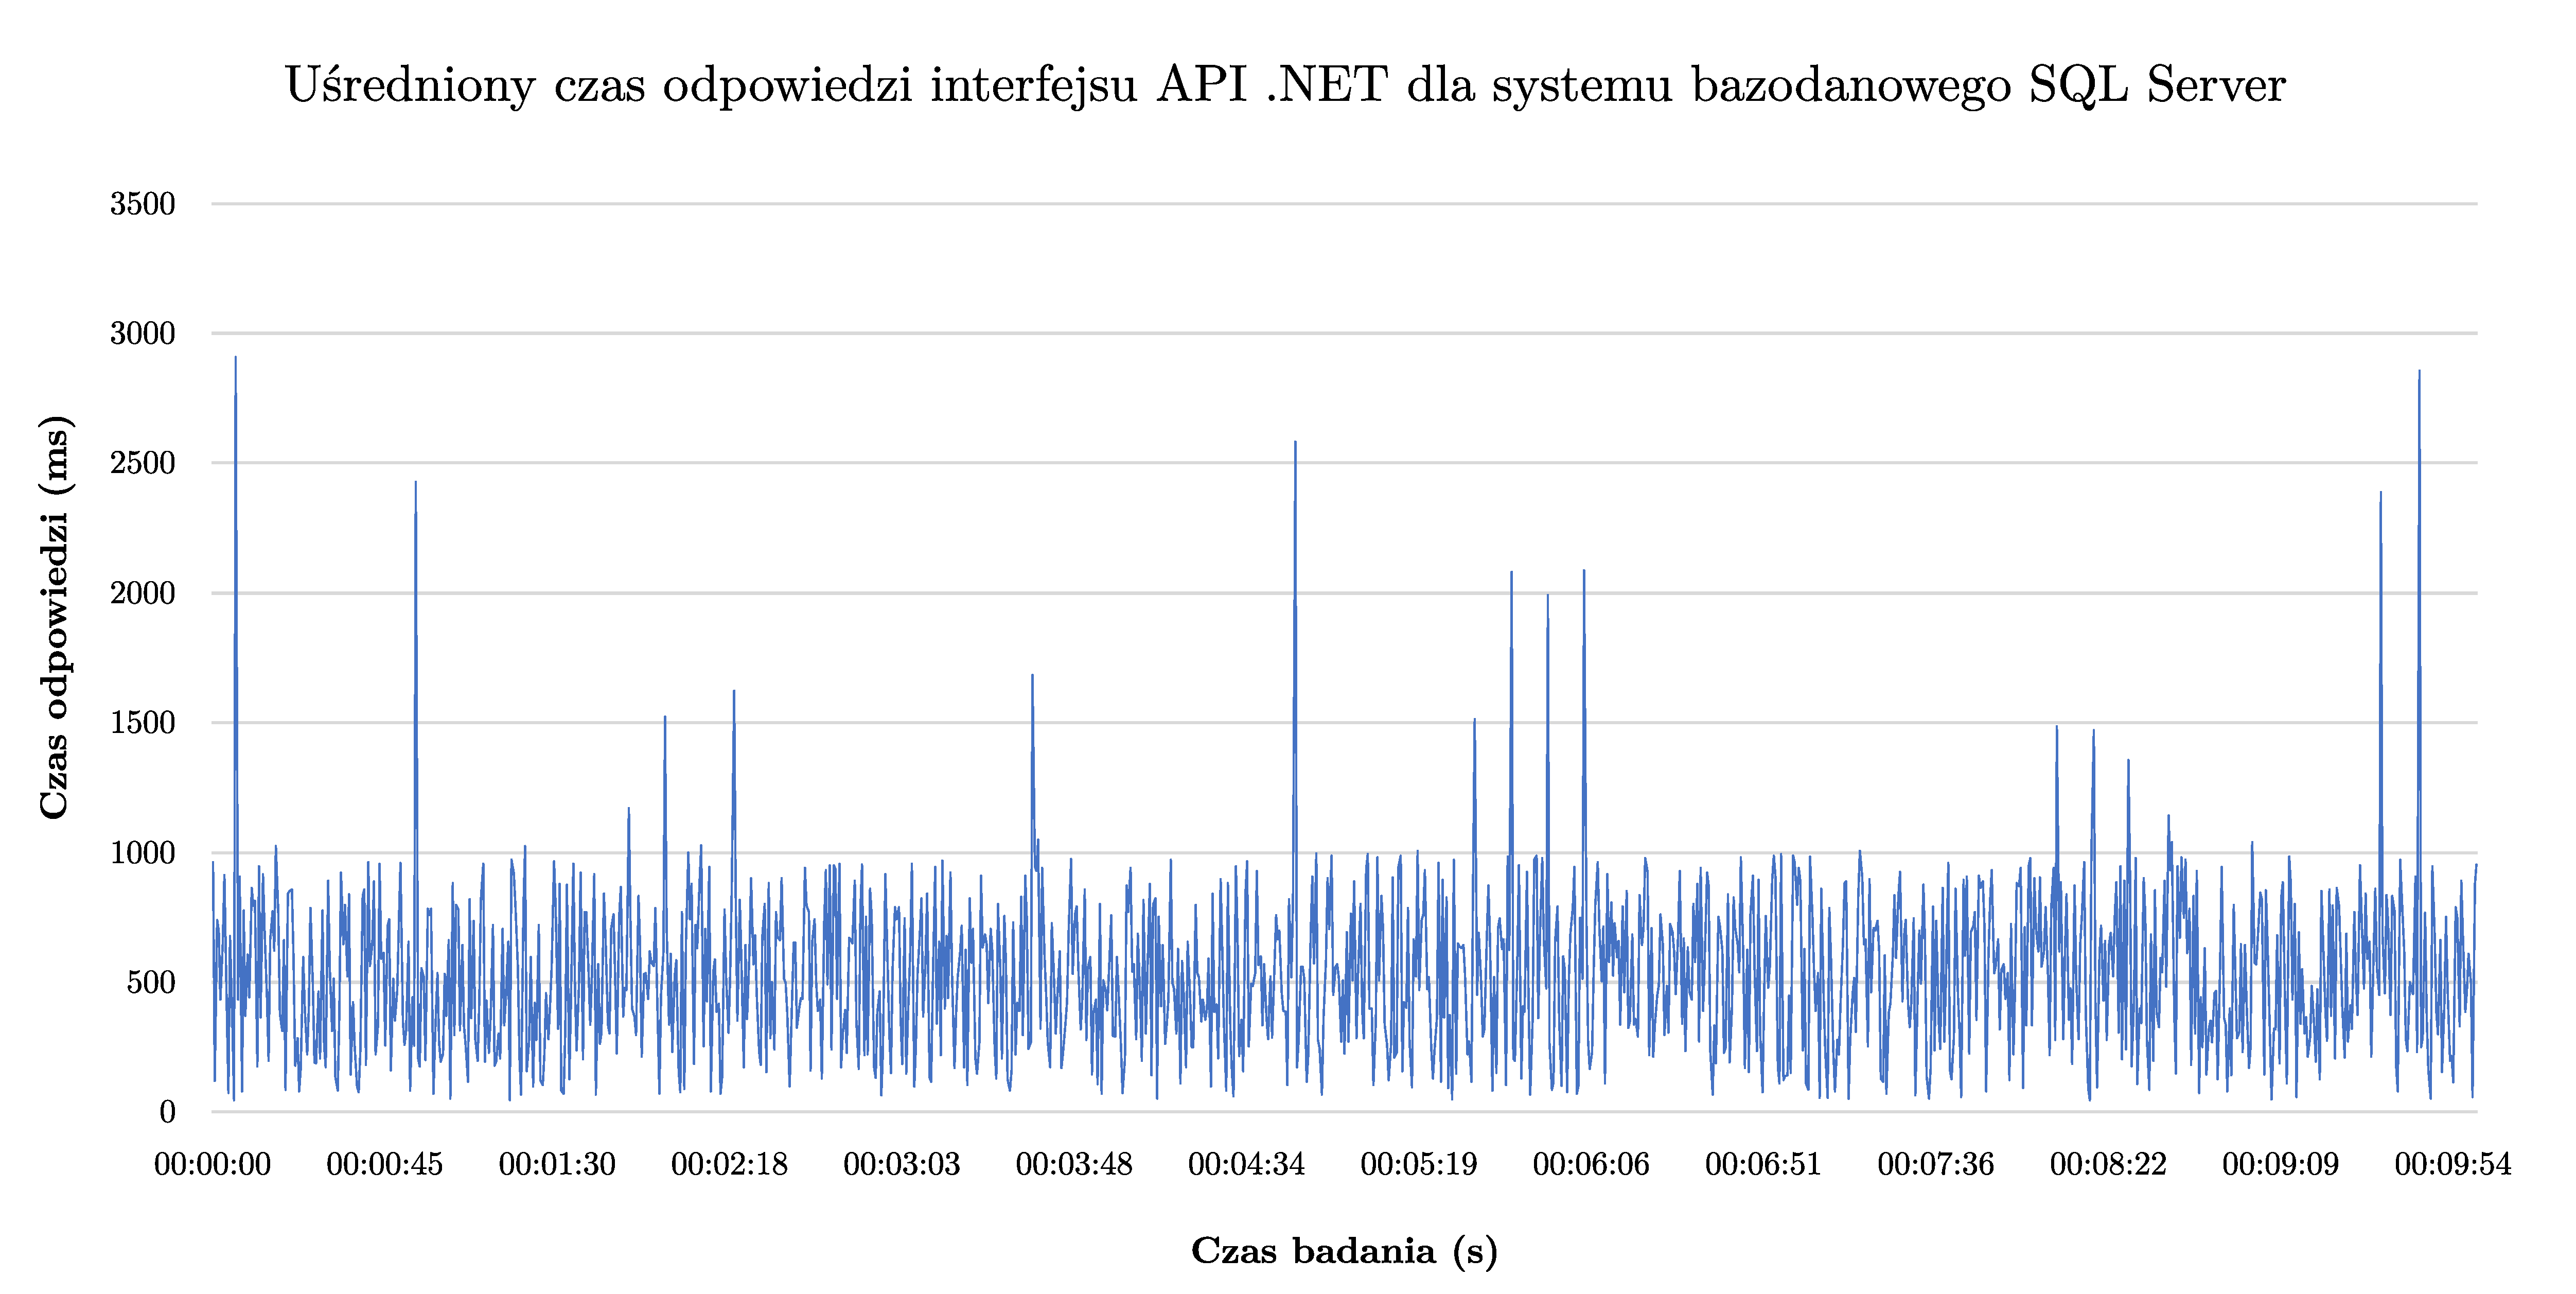
\includegraphics[width=\linewidth]{rys05/testy-funkcjonalne-dotnet.pdf}
    \caption{Rzeczywisty pomiar chwilowy czasu odpowiedzi na żądanie dla konfiguracji .NET/SQL Server w kontekście testu funkcjonalnego}
    \label{fig:wykres-testy-funkcjonalne-dotnet}
\end{figure}

Na podstawie analogicznych danych, dla każdej pary interfejs API -- system bazodanowy, zdefiniowano progi tolerancji oraz frustracji stanowiące punkty odniesienia przy kalkulacji wartości wskaźnika APDEX. Wartości te, ustalono poprzez rosnące posortowanie zbioru czasów odpowiedzi API, a następnie dokonanie symetrycznego podziału dwupunktowego.

Uzyskane przedziały satysfakcji, tolerancji oraz frustracji względem każdego systemu bazodanowego oraz technologii tworzenia API zostały zobrazowane na wykresach \ref{fig:apdex-dotnet} oraz \ref{fig:apdex-nodejs}.

\begin{figure}[htb]
    \centering
     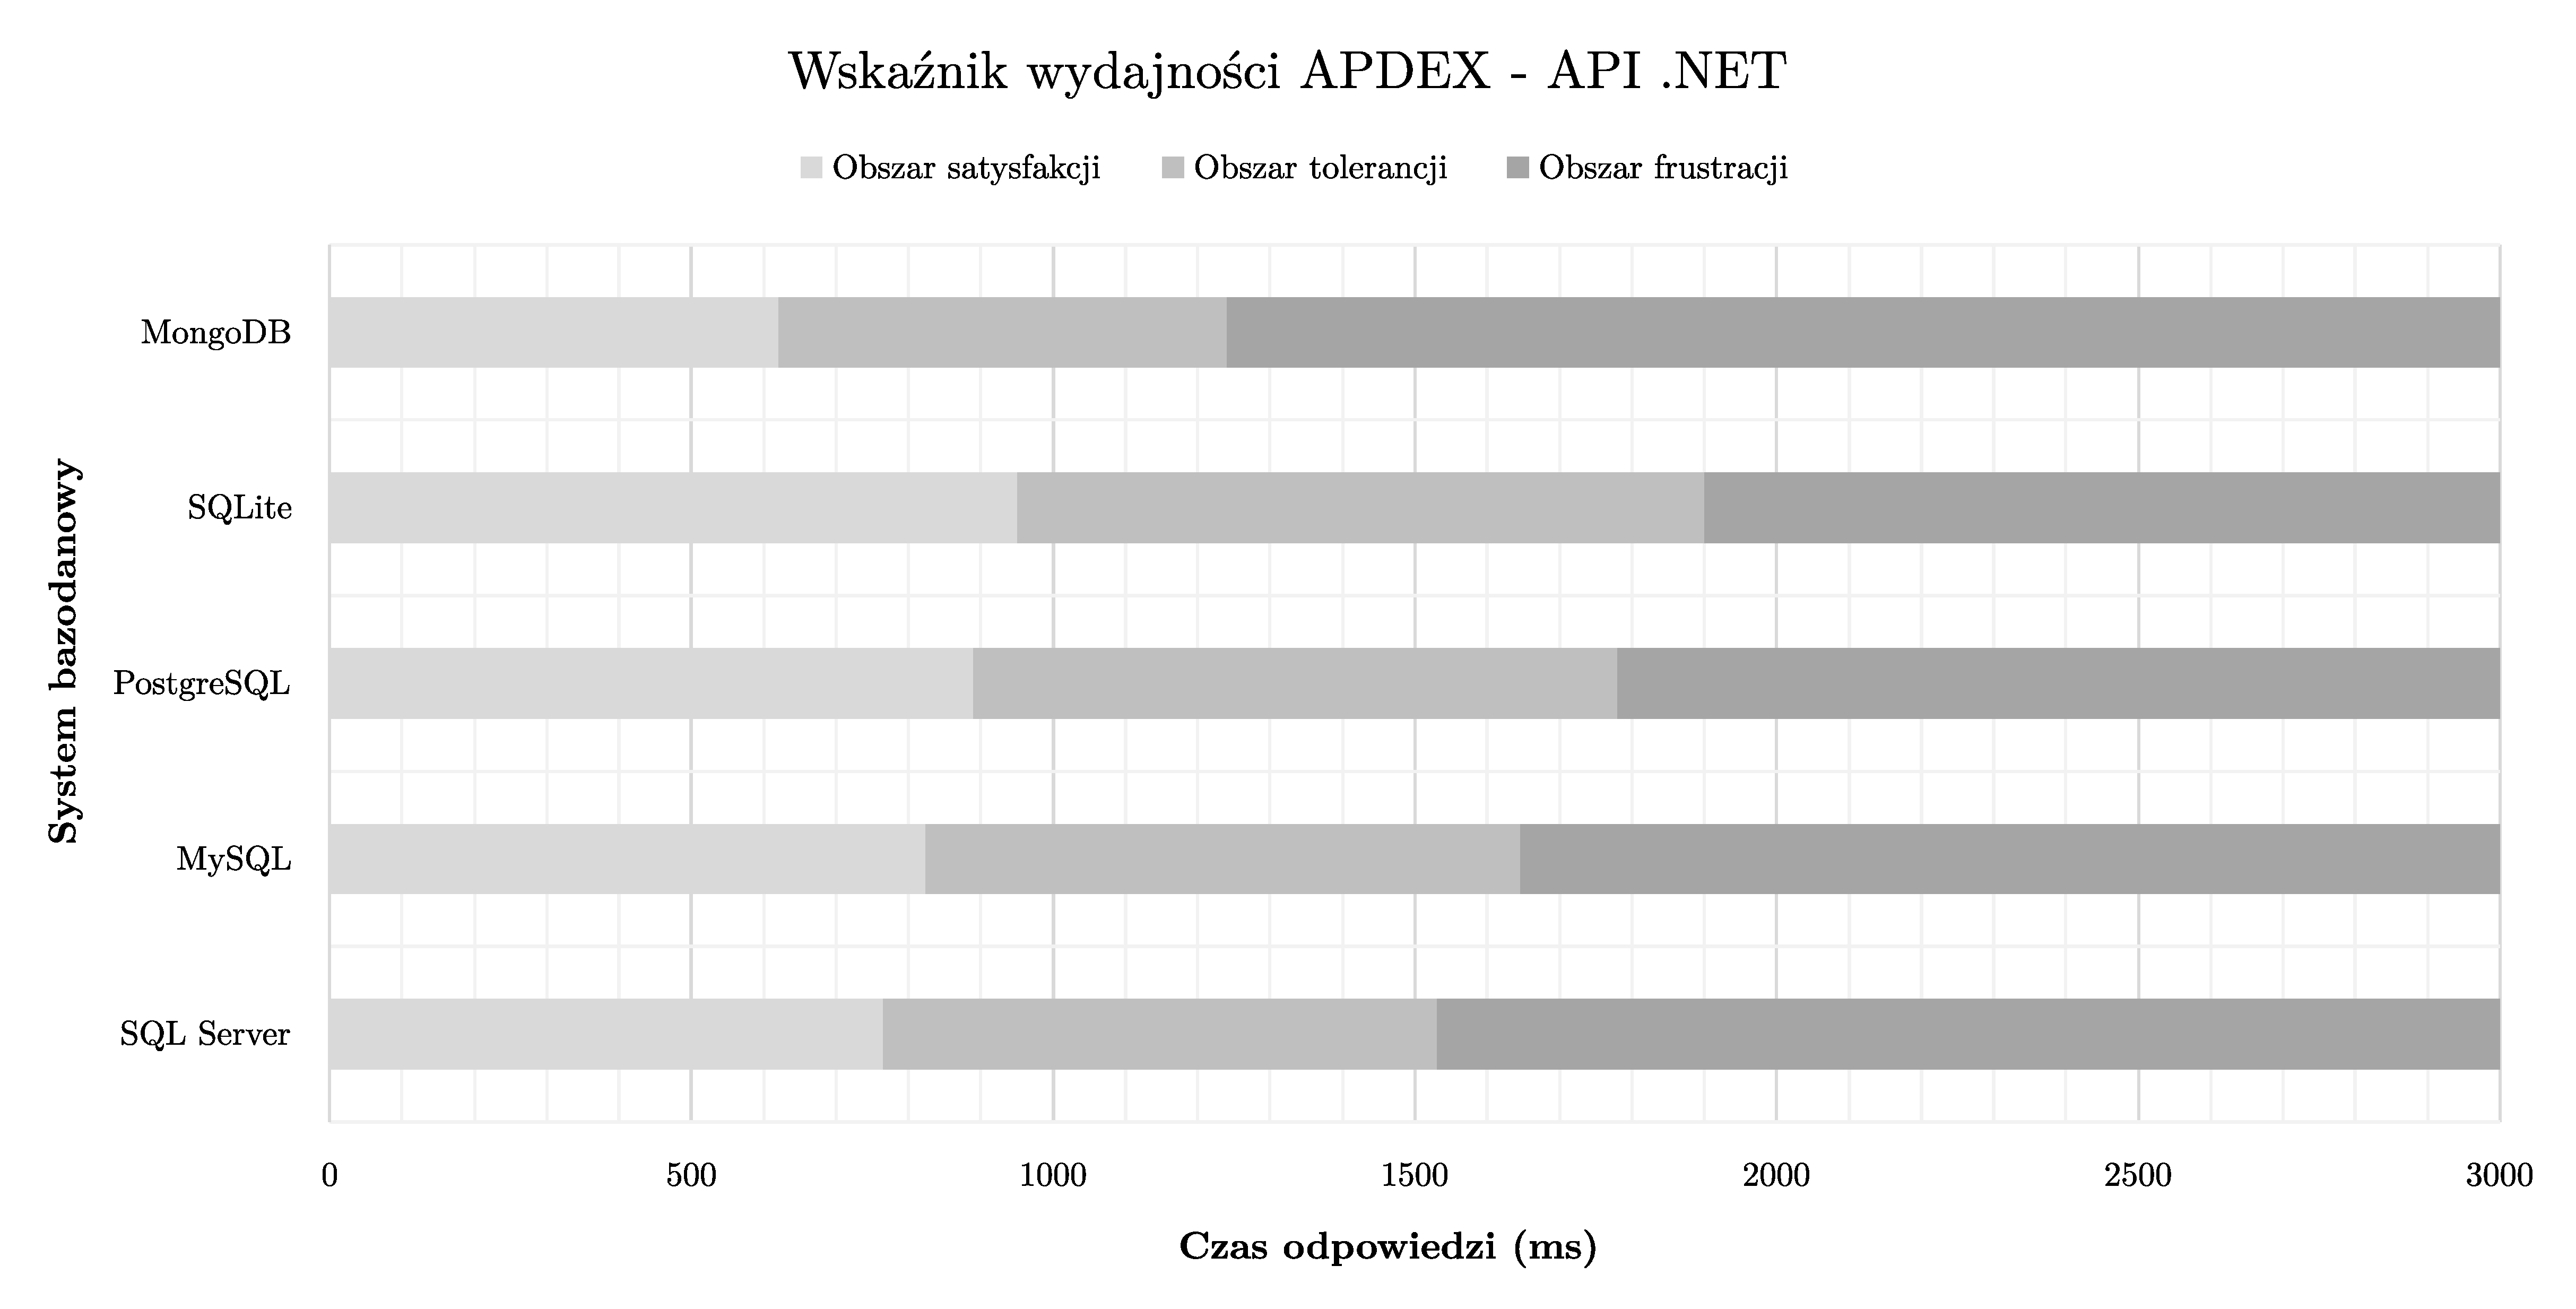
\includegraphics[width=\linewidth]{rys05/apdex-dotnet.pdf}
    \caption{Obszary satysfakcji, tolerancji oraz frustracji wskaźnika APDEX względem poszczególnych systemów bazodanowych dla API zaimplementowanego w C\#}
    \label{fig:apdex-dotnet}
\end{figure}

\clearpage

\begin{figure}[htb]
    \centering
     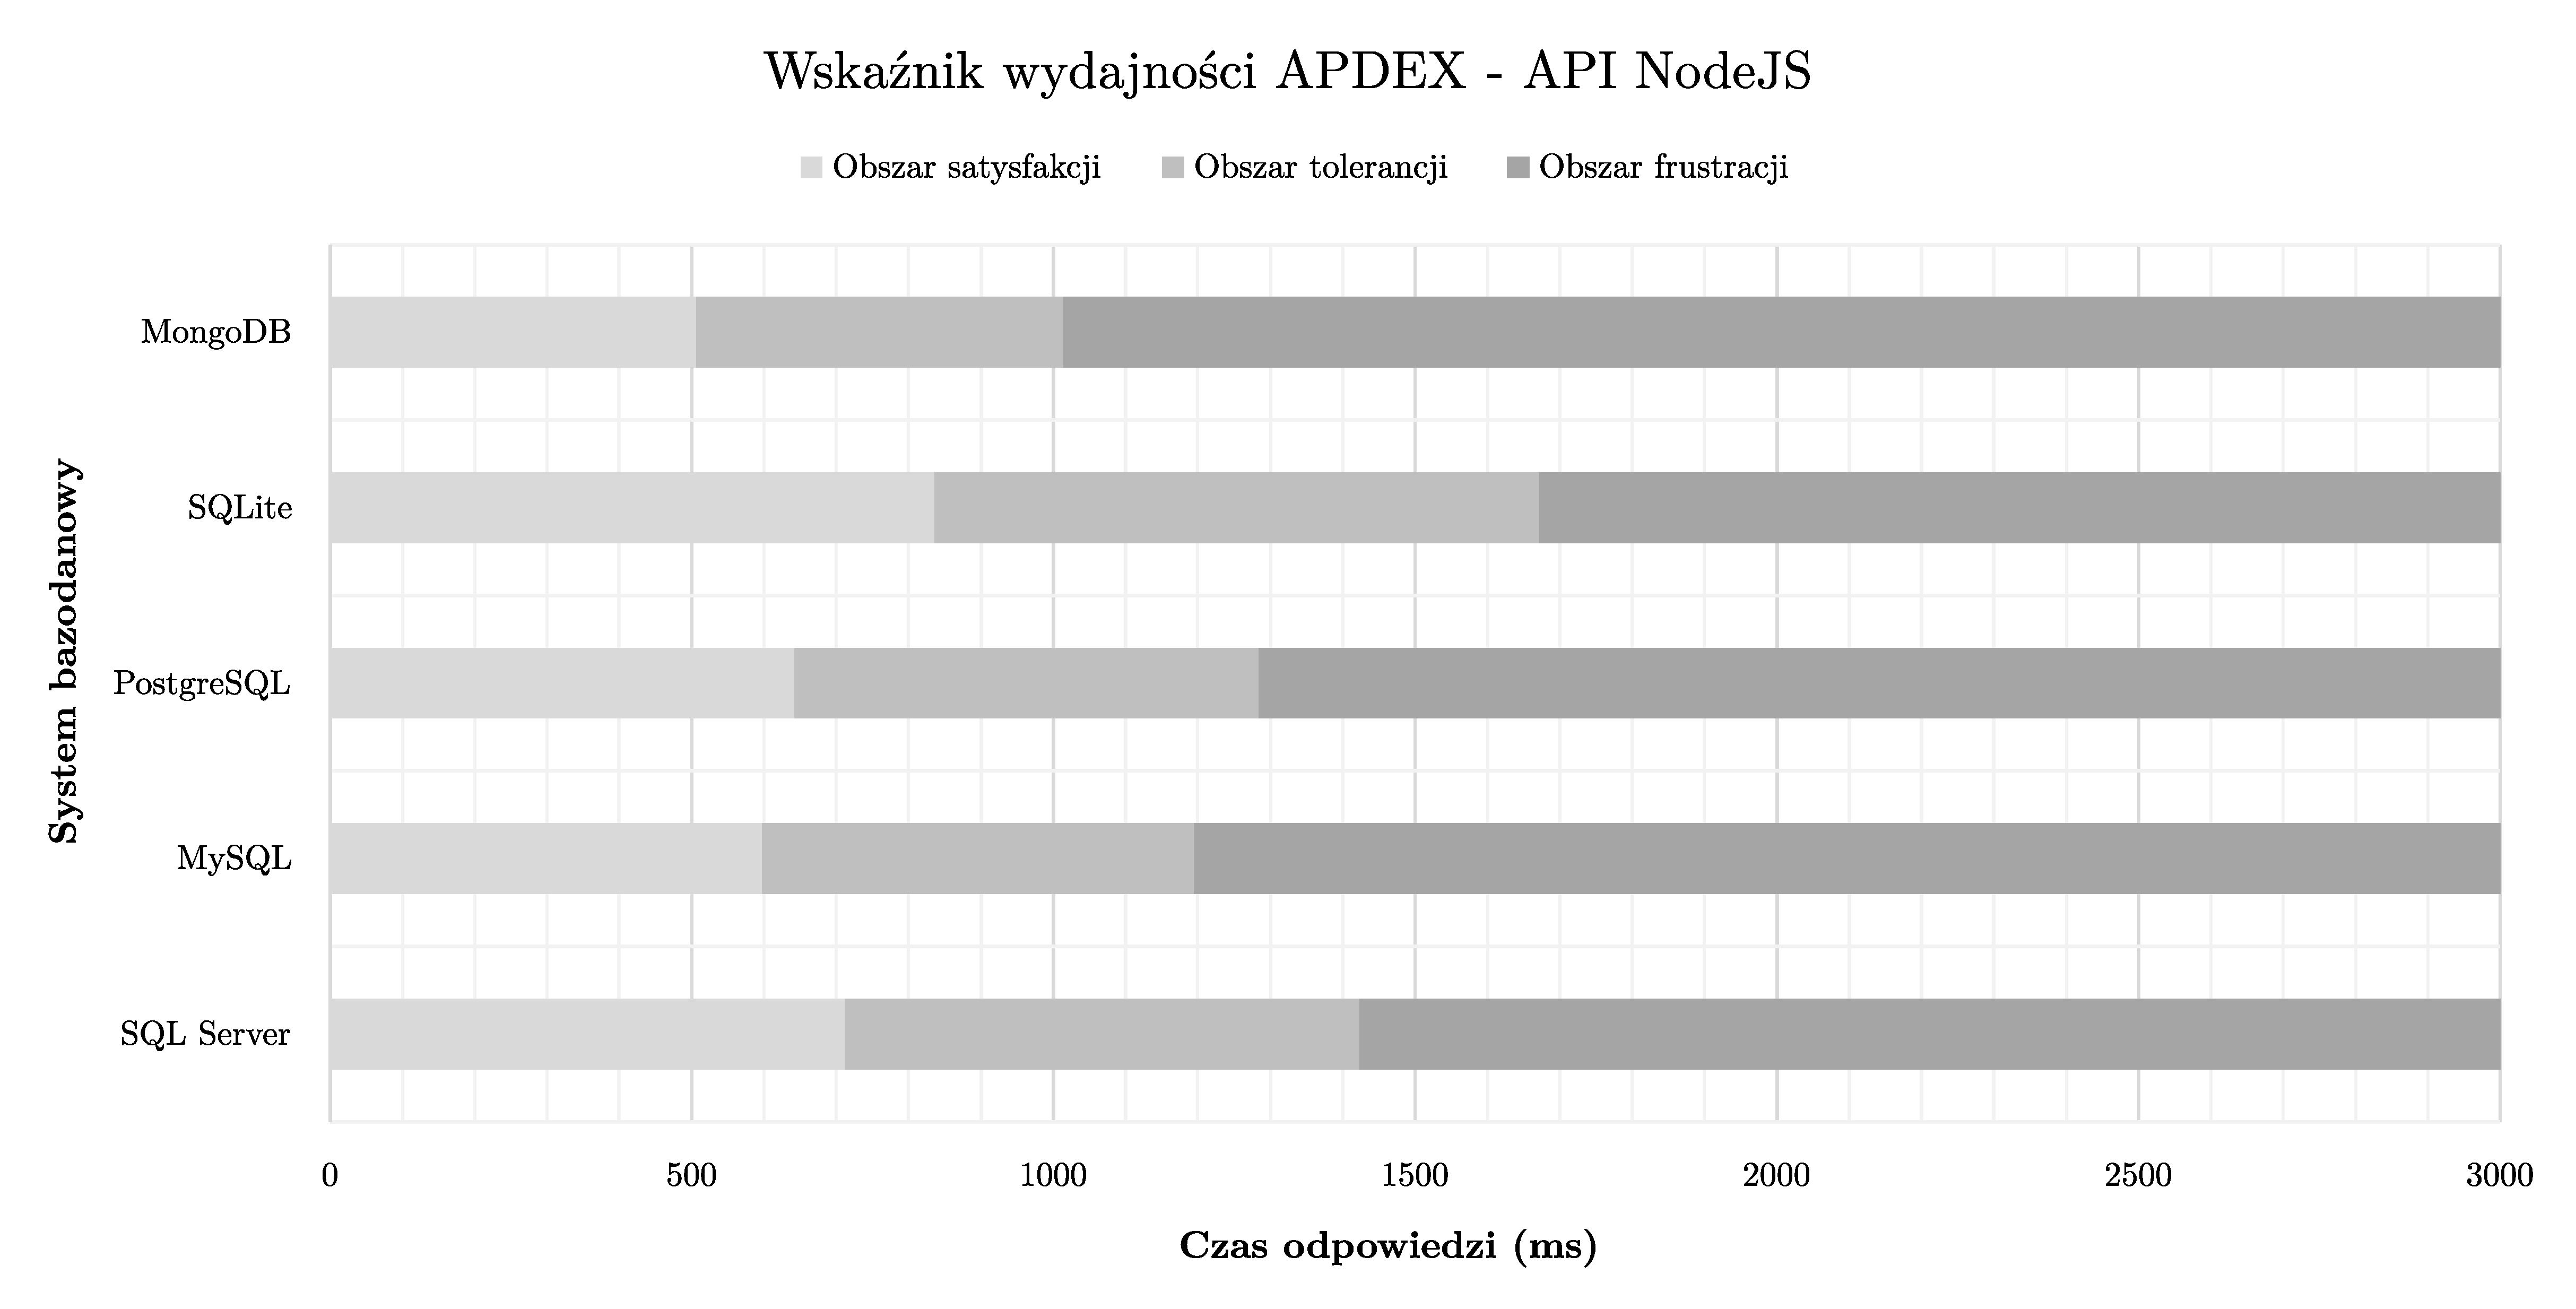
\includegraphics[width=\linewidth]{rys05/apdex-nodejs.pdf}
    \caption{Obszary satysfakcji, tolerancji oraz frustracji wskaźnika APDEX względem poszczególnych systemów bazodanowych dla API zaimplementowanego w JavaScript}
    \label{fig:apdex-nodejs}
\end{figure}

Po spełnieniu warunków początkowych badania zrealizowano faktyczne czynności badawcze. Wykorzystując lokalną topologię fizyczną nr 1, omówioną w ramach sekcji \ref{sec:lokalne-srodowisko-badawcze-ver-1} rozpoczęto generowanie żądań protokołu hipertekstowego wytwarzanych przez dwa równolegle pracujące hosty sieciowe. Procedura badawcza trwała 20 minut i polegała na stopniowym zwiększaniu liczby współbieżnie pracujących procesów oprogramowania testującego rozpoczynając od jednego procesu a kończąc na pięciu tysiącach. Nowe wątki oprogramowania Apache JMeter uruchamiane były w stałych odstępach czasu, co implikuje niezmienność długości przedziału czasowego pracy w obrębie ustalonej liczby wątków. Czas ten, wynosi 240 ms. Przy uwzględnieniu minimalnej zaobserwowanej średniej wartości natężenia generowanych żądań, wynoszącej 152 zapytania w ciągu sekundy, liczebność zbioru próbek czasu zapytania w odniesieniu do dowolnego z 4990 poziomów przyrostu ruchu wyniosła co najmniej 36 elementów. Pierwsze 10 poziomów dotyczących liczby klientów generujących komunikaty nie pozwoliło na zarejestrowanie co najmniej 30 próbek, przez co elementy te, nie były brane pod uwagę w czasie opracowywania uzyskanych wyników. Opisane w niniejszym akapicie czynności zostały wykonane względem interfejsów programowania aplikacji wykorzystujących porównywane technologie, uwzględniając komunikację z każdym z pięciu systemów bazodanowych.

Na wykresach \ref{fig:response-mtc-1} a) do \ref{fig:response-mtc-1} j) zaprezentowano uśrednione względem liczby pracujących wątków, czasy odpowiedzi na żądanie generowane w kierunku ewaluowanych interfejsów API.

Analizując wyniki uzyskane dla operacji pobierania kolekcji obiektów, zauważyć można niewielkie różnice w wartości średnich czasów odpowiedzi, występujące w przedziale do około 4000 użytkowników. Różnice te, nie faworyzują ani deprecjonują któregokolwiek z rozwiązań.

\begin{figure}[H]
  \centering
	\begin{tabular}{@{}ll@{}}
    a) & b) \\
    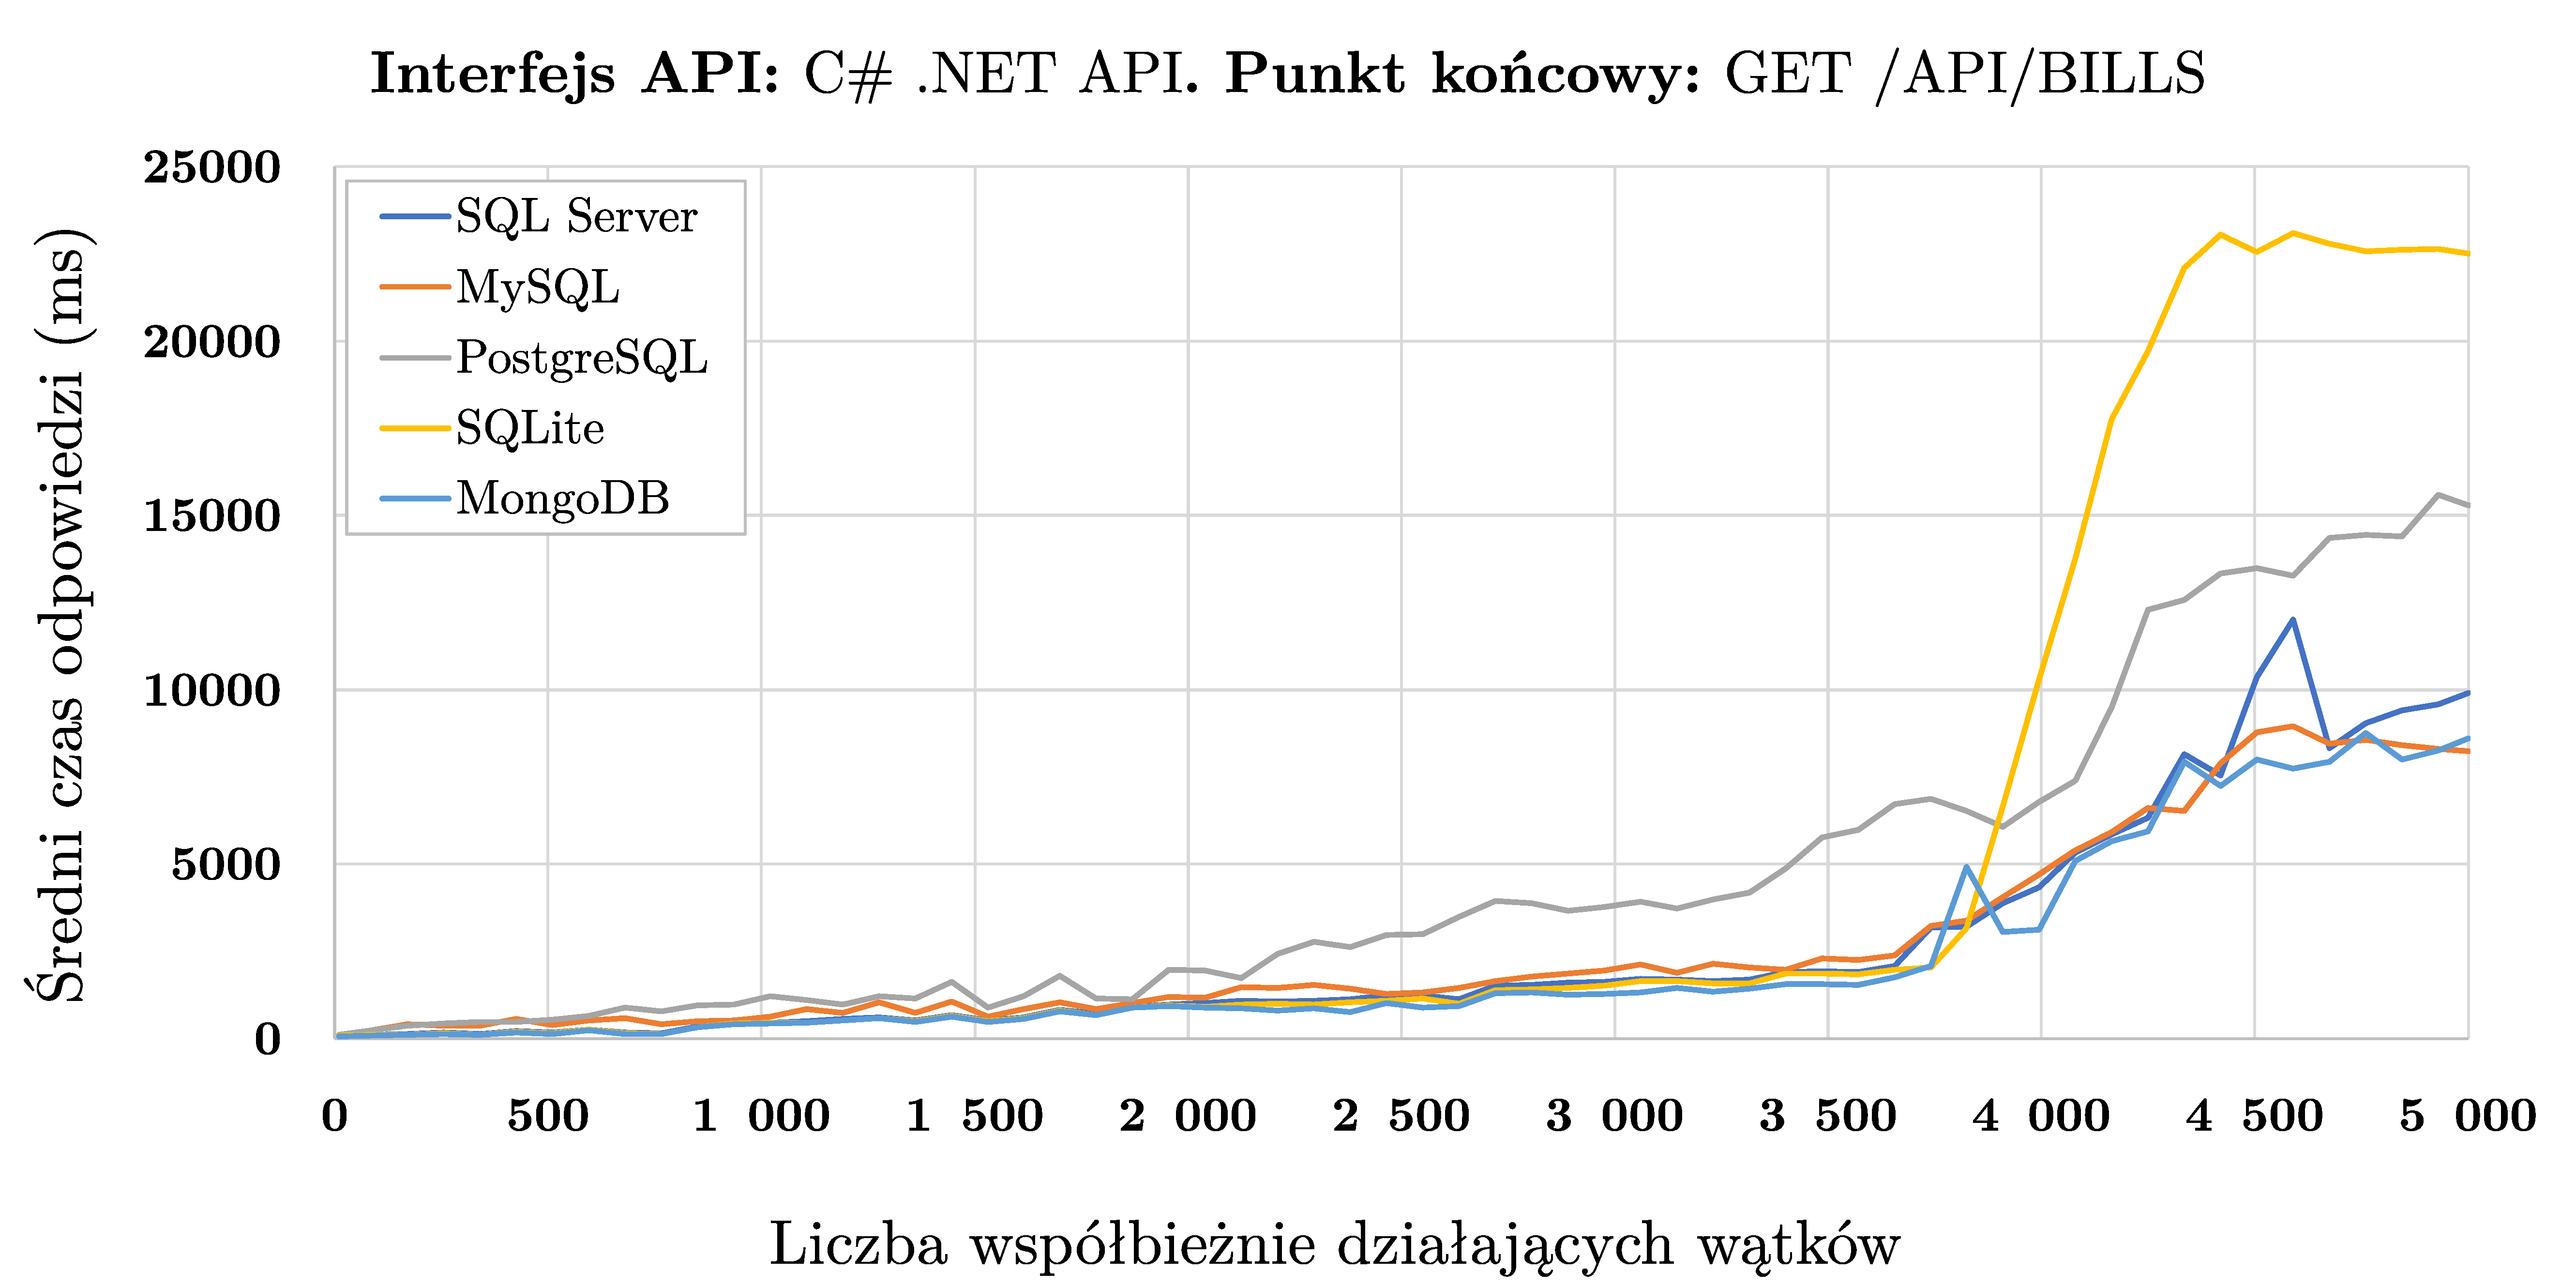
\includegraphics[width=0.49\textwidth]{rys05/response-dotnet-fetchAllBills.pdf} & 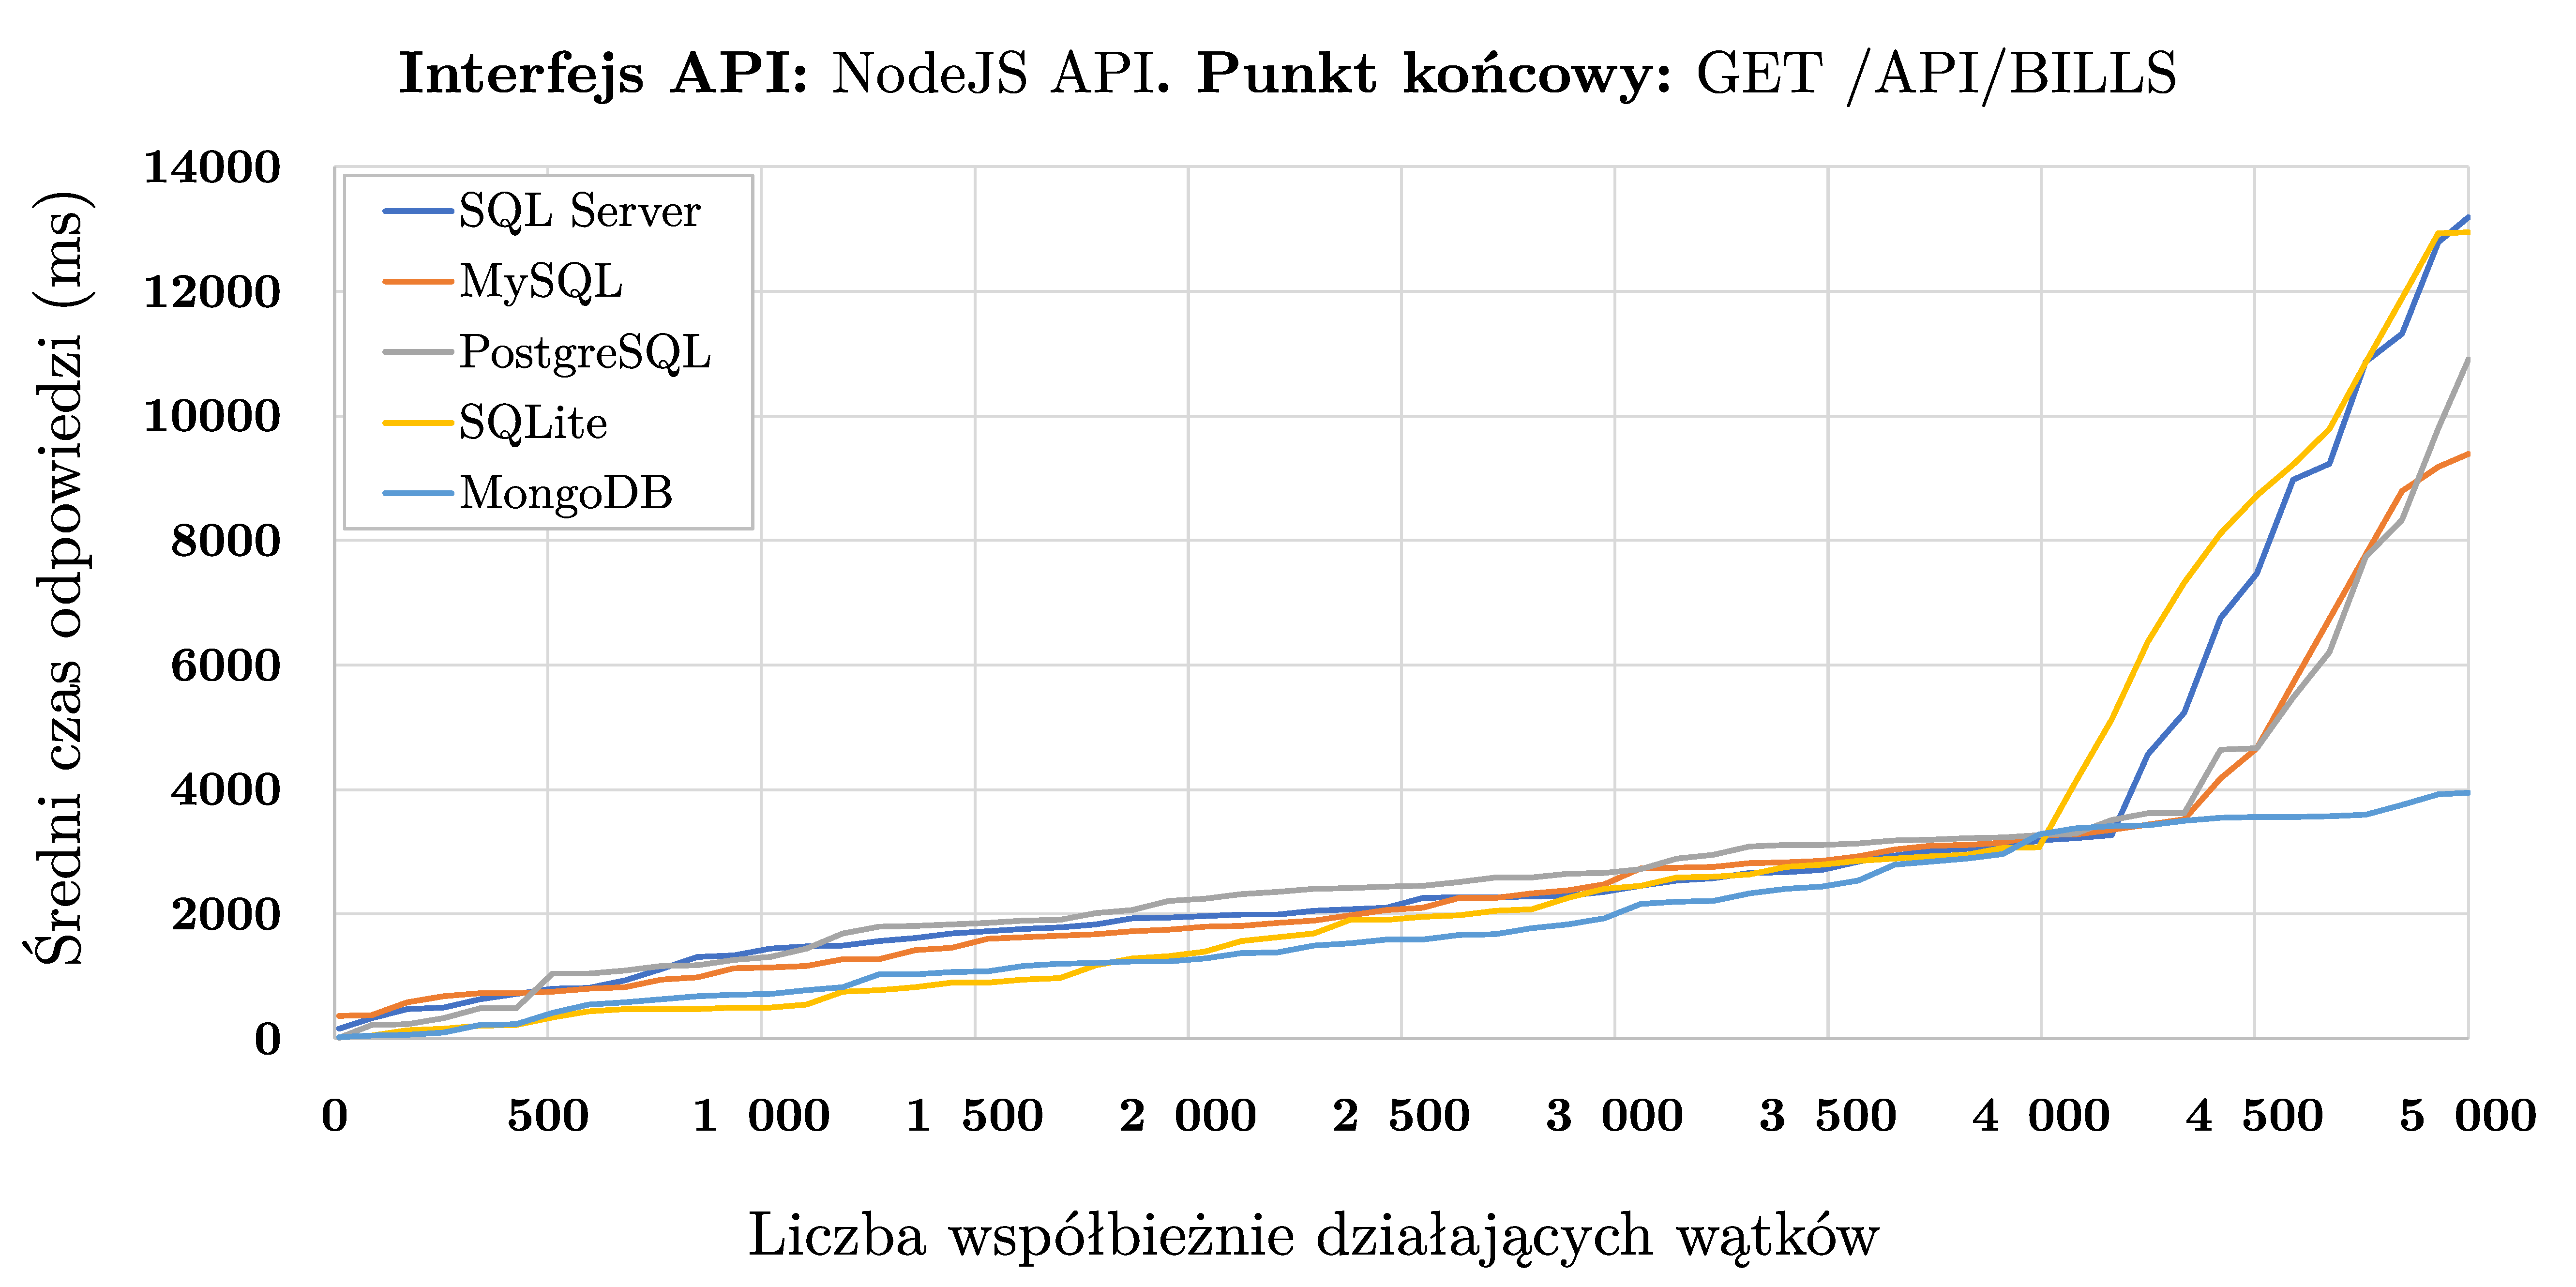
\includegraphics[width=0.49\textwidth]{rys05/response-nodejs-fetchAllBills.pdf} \\
    c) & d) \\
    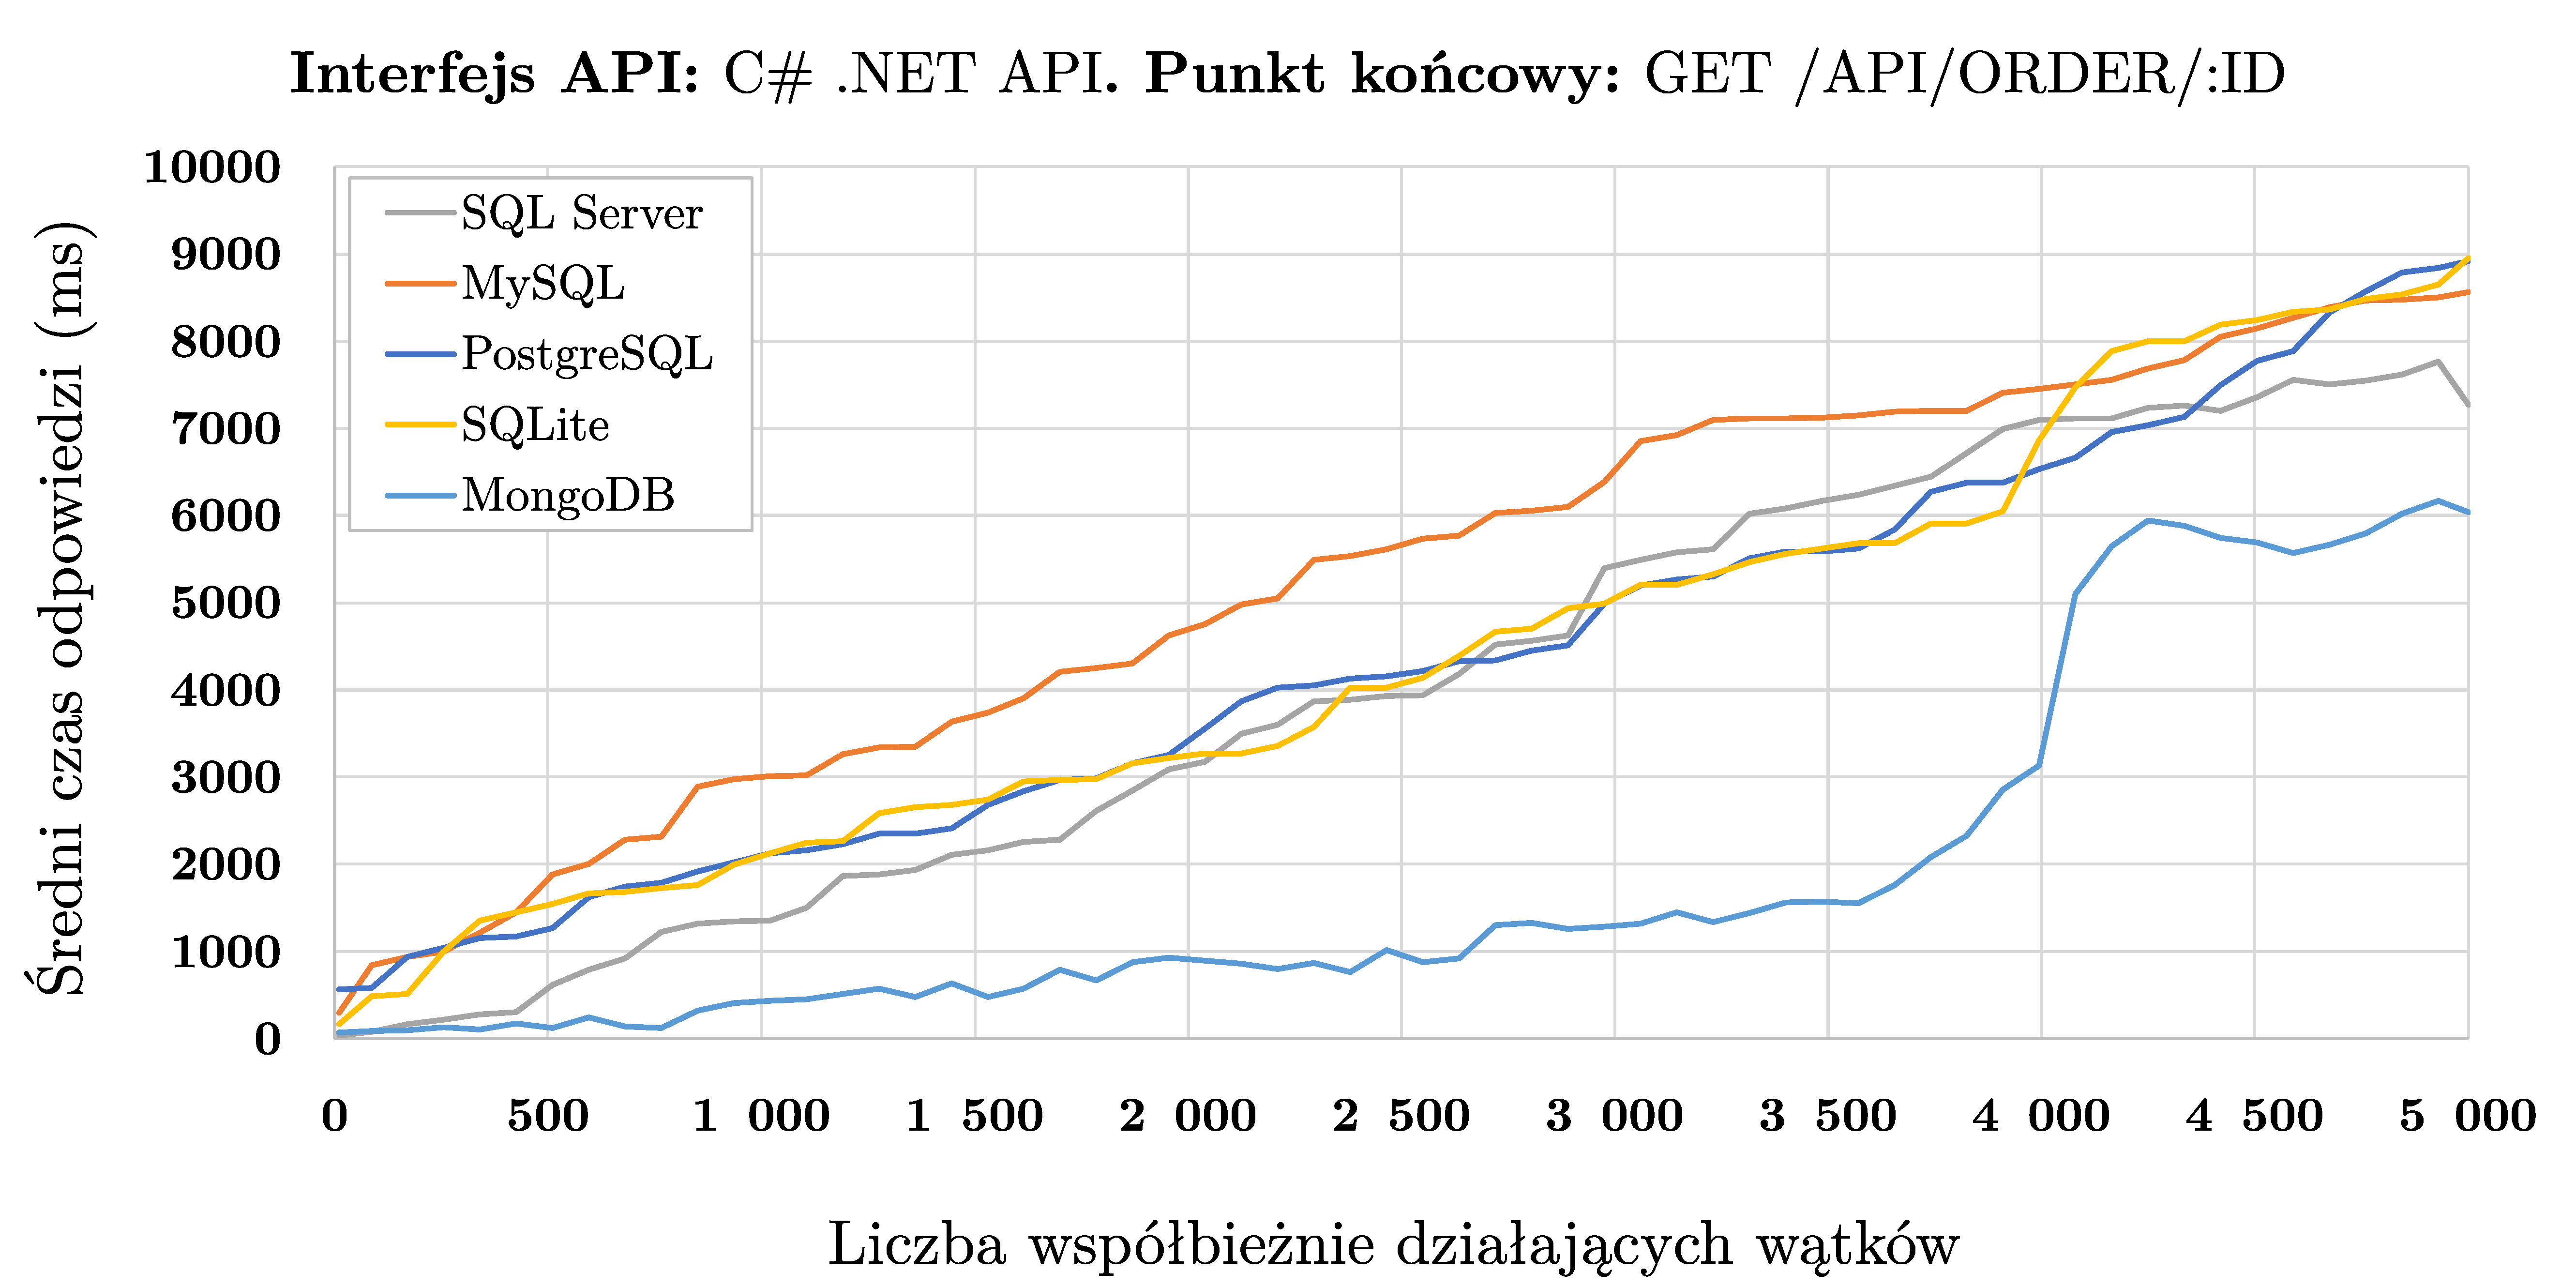
\includegraphics[width=0.49\textwidth]{rys05/response-dotnet-getSingleOrder.pdf} & 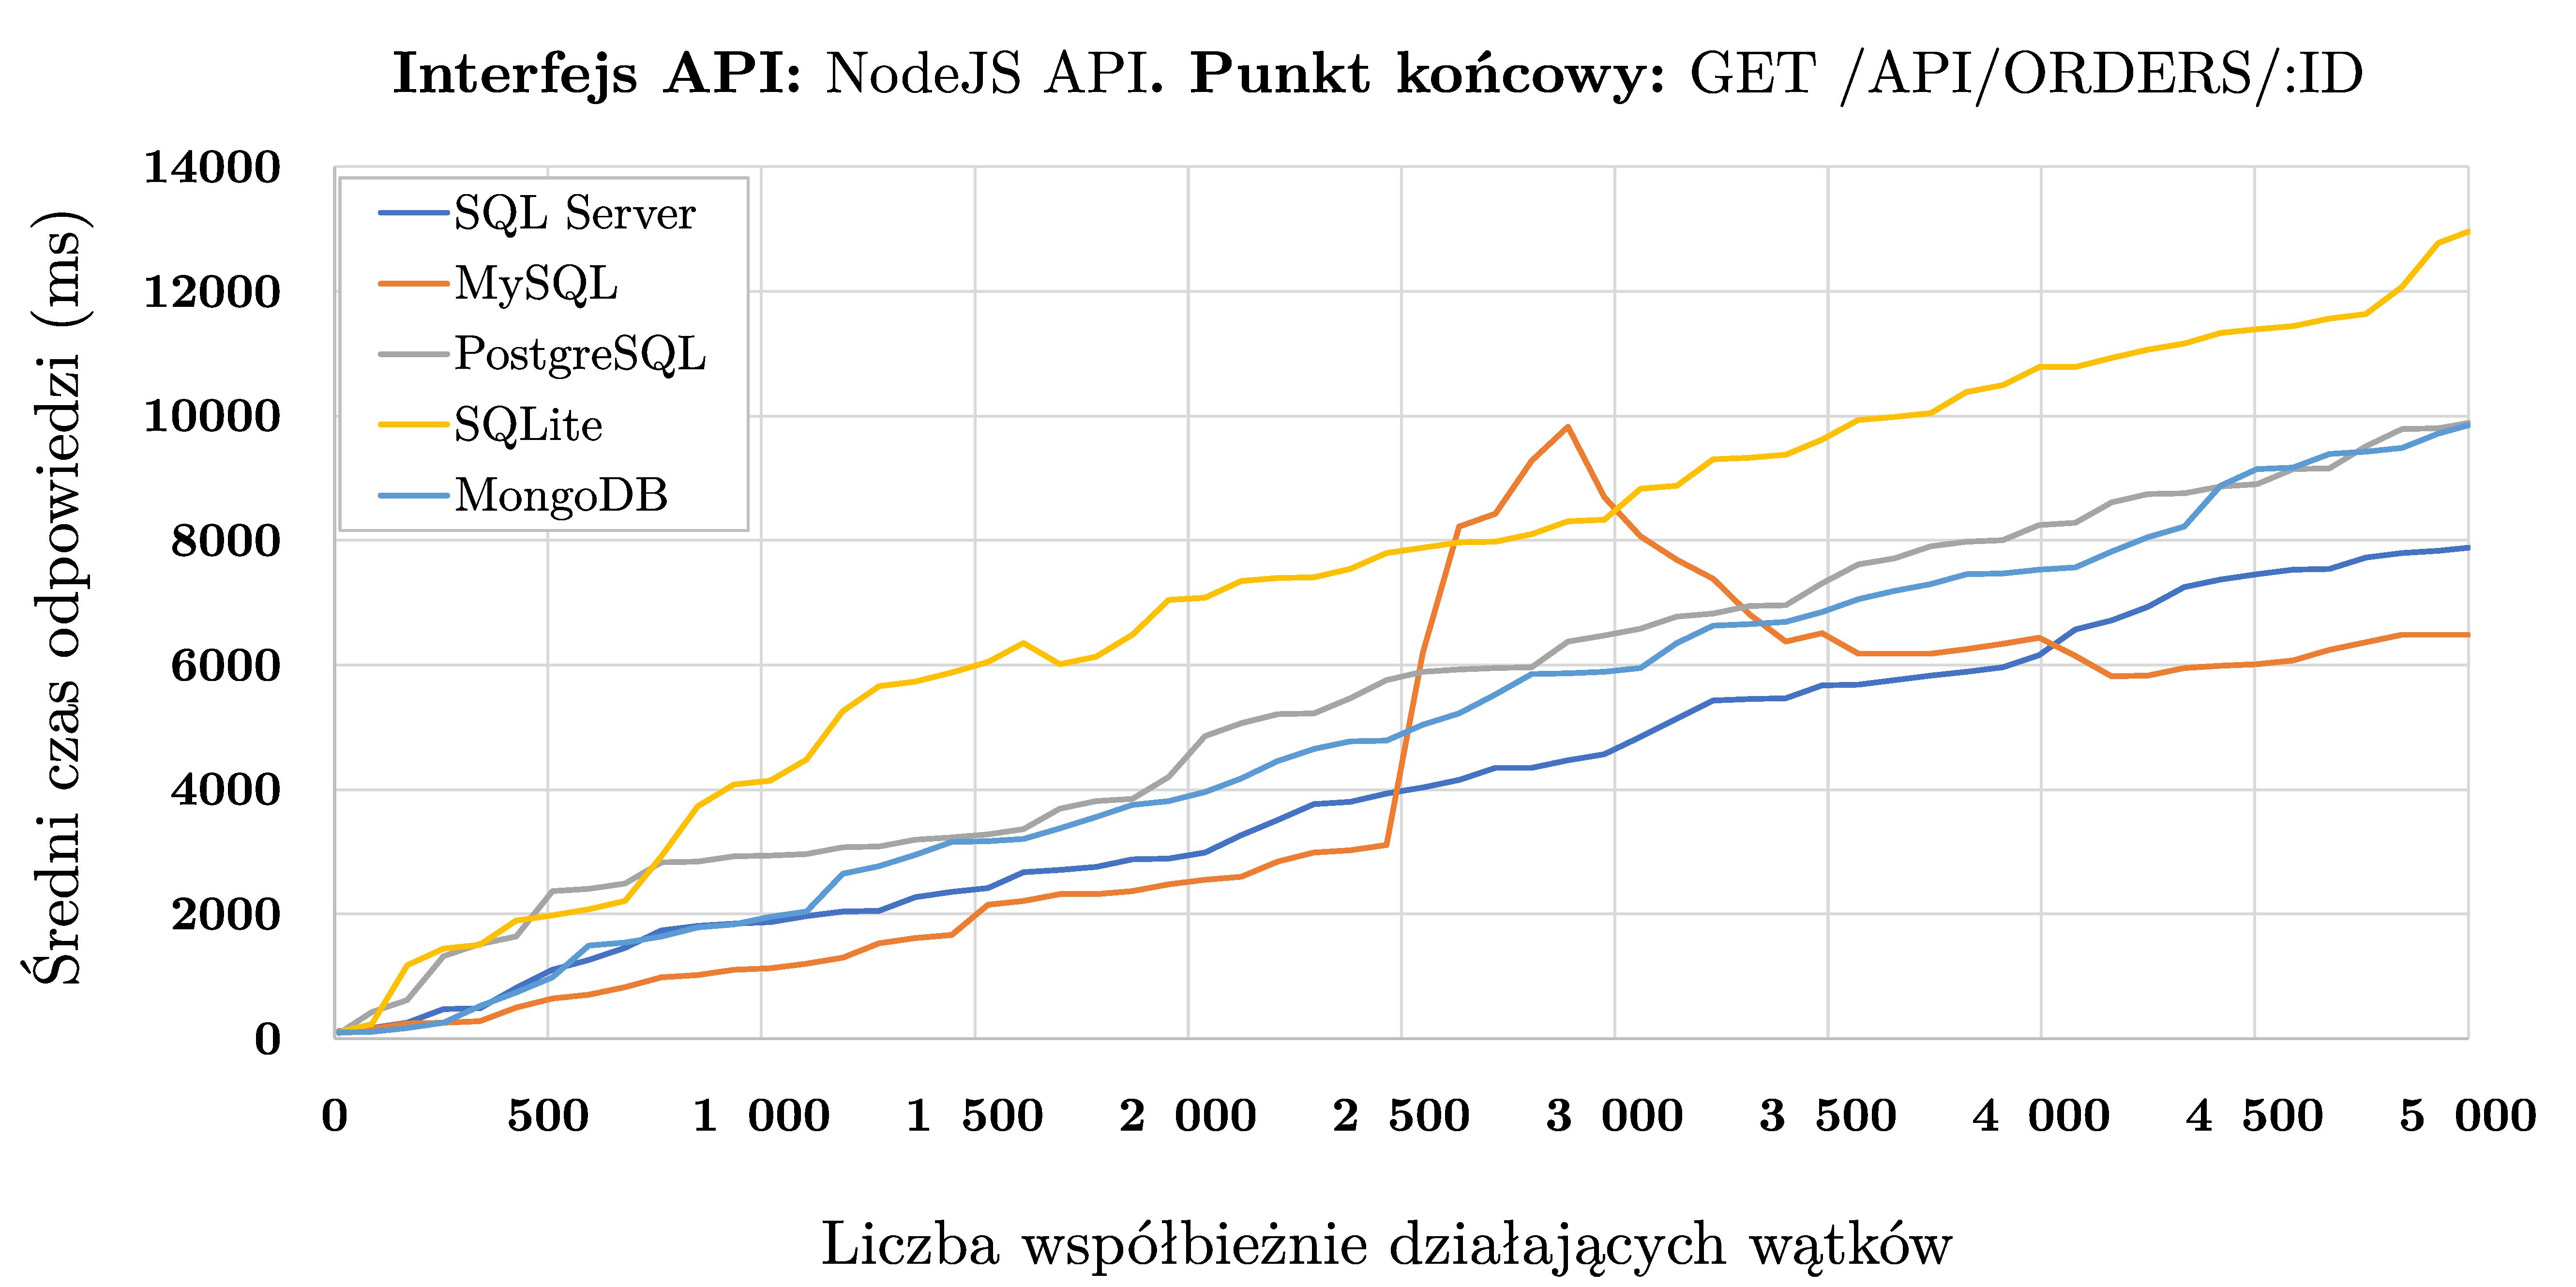
\includegraphics[width=0.49\textwidth]{rys05/response-nodejs-getSingleOrder.pdf} \\
    e) & f) \\
    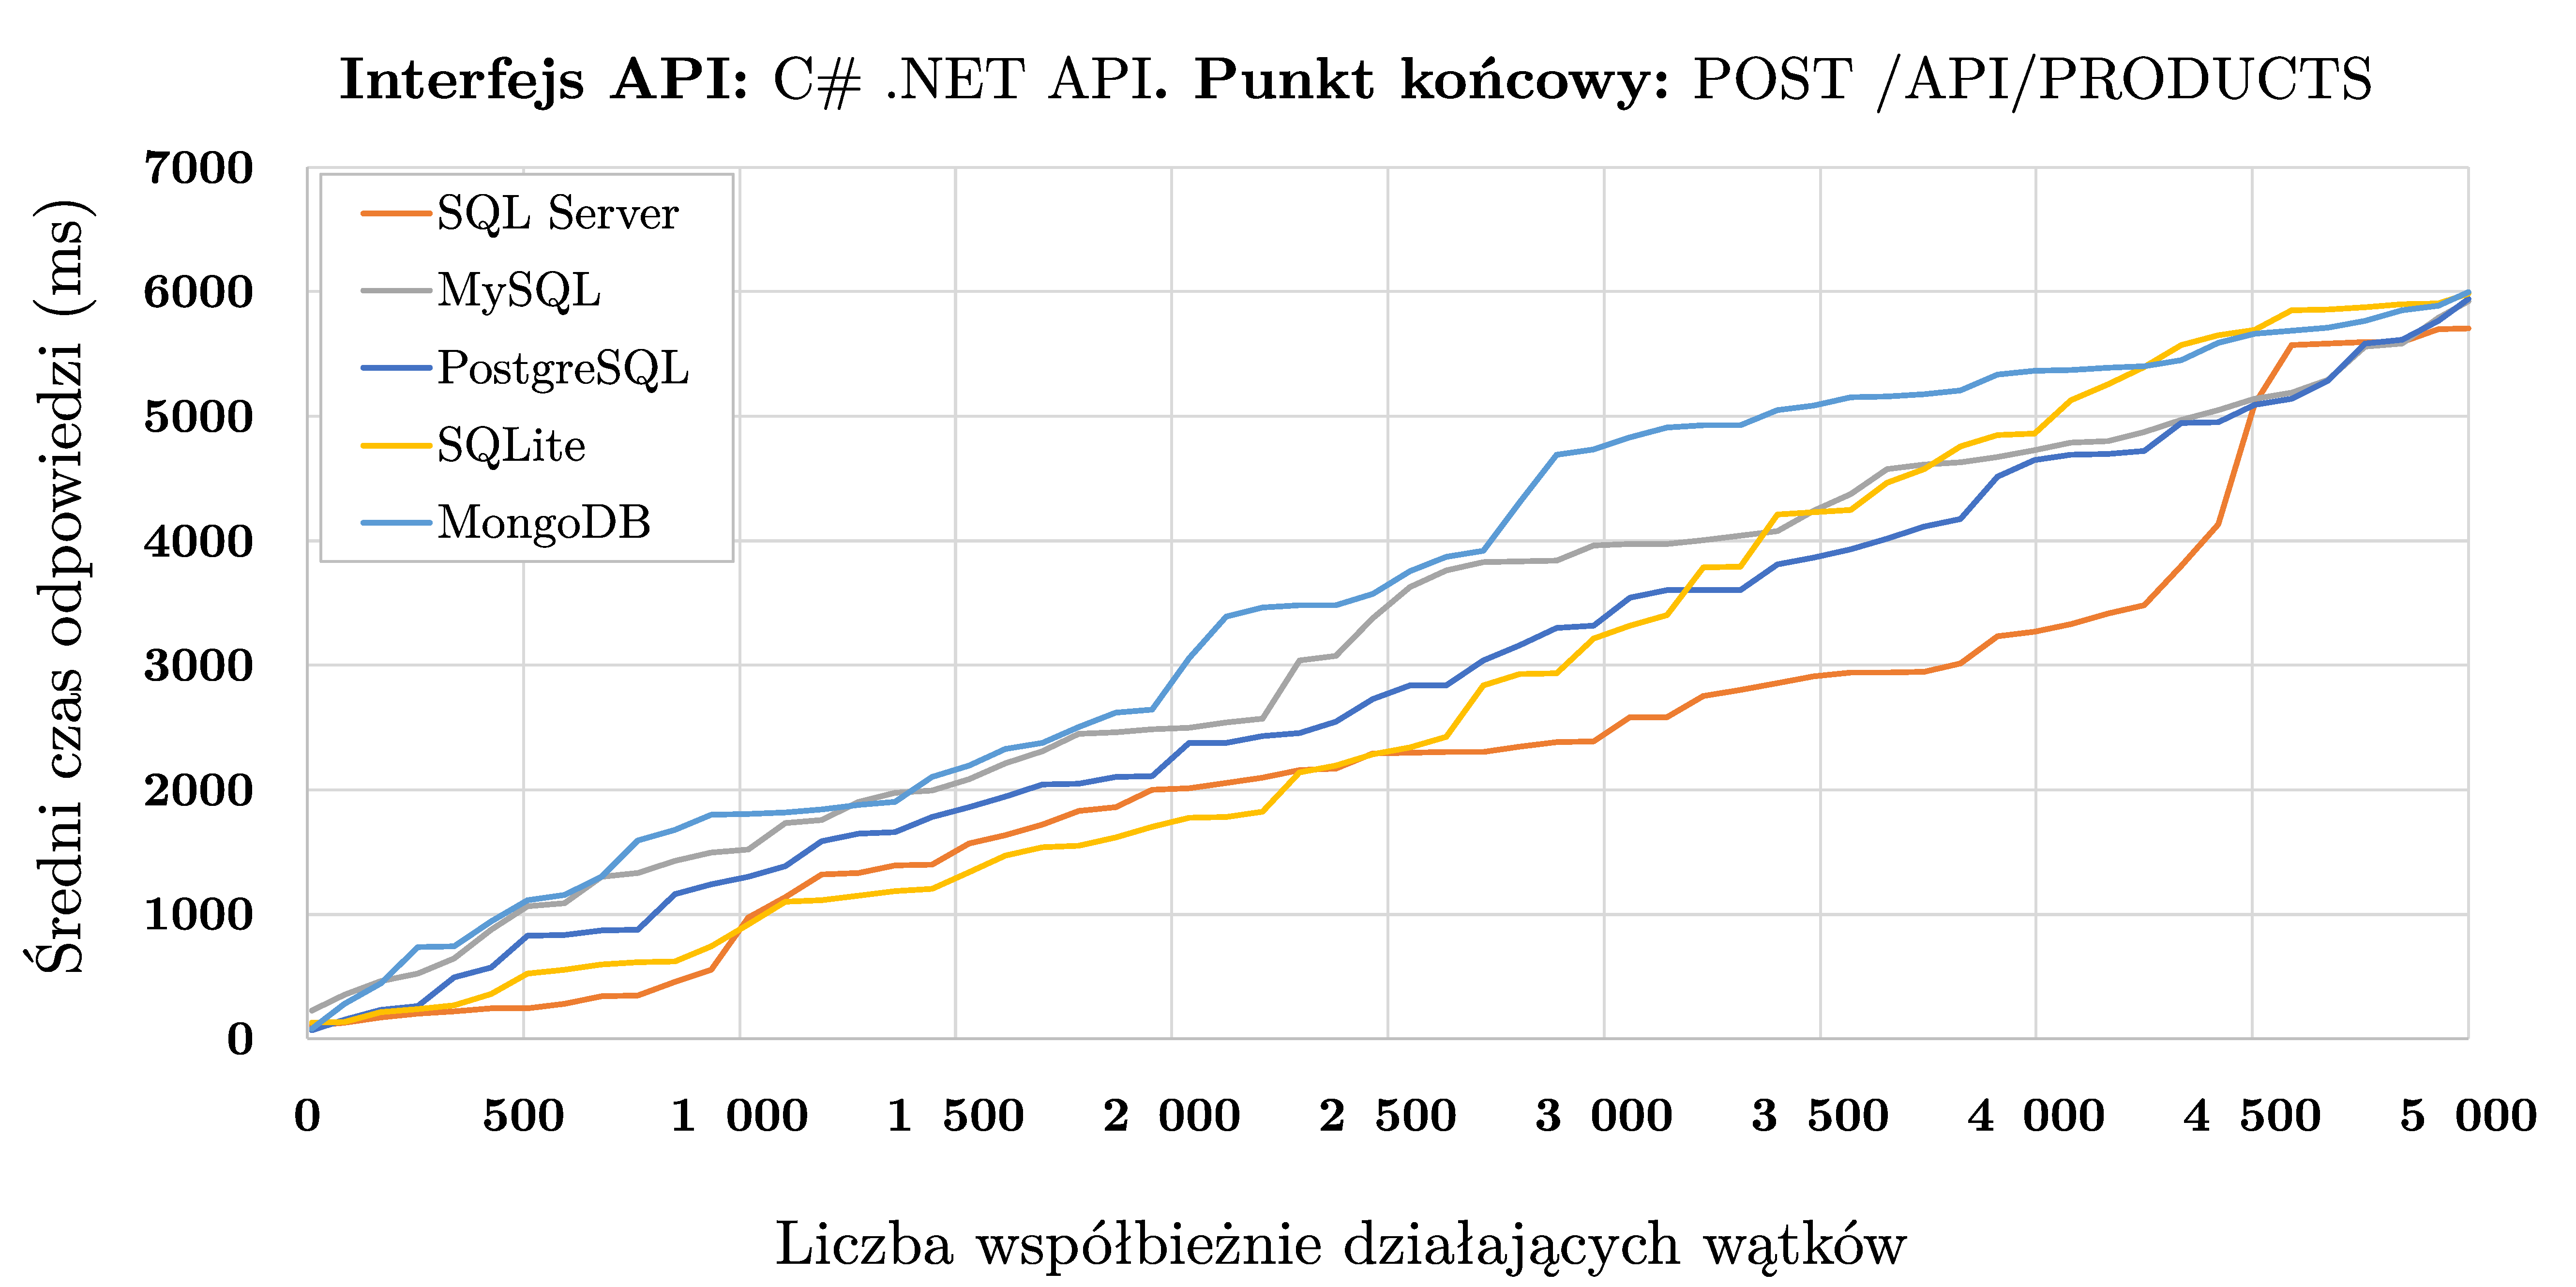
\includegraphics[width=0.49\textwidth]{rys05/response-dotnet-addProduct.pdf} & 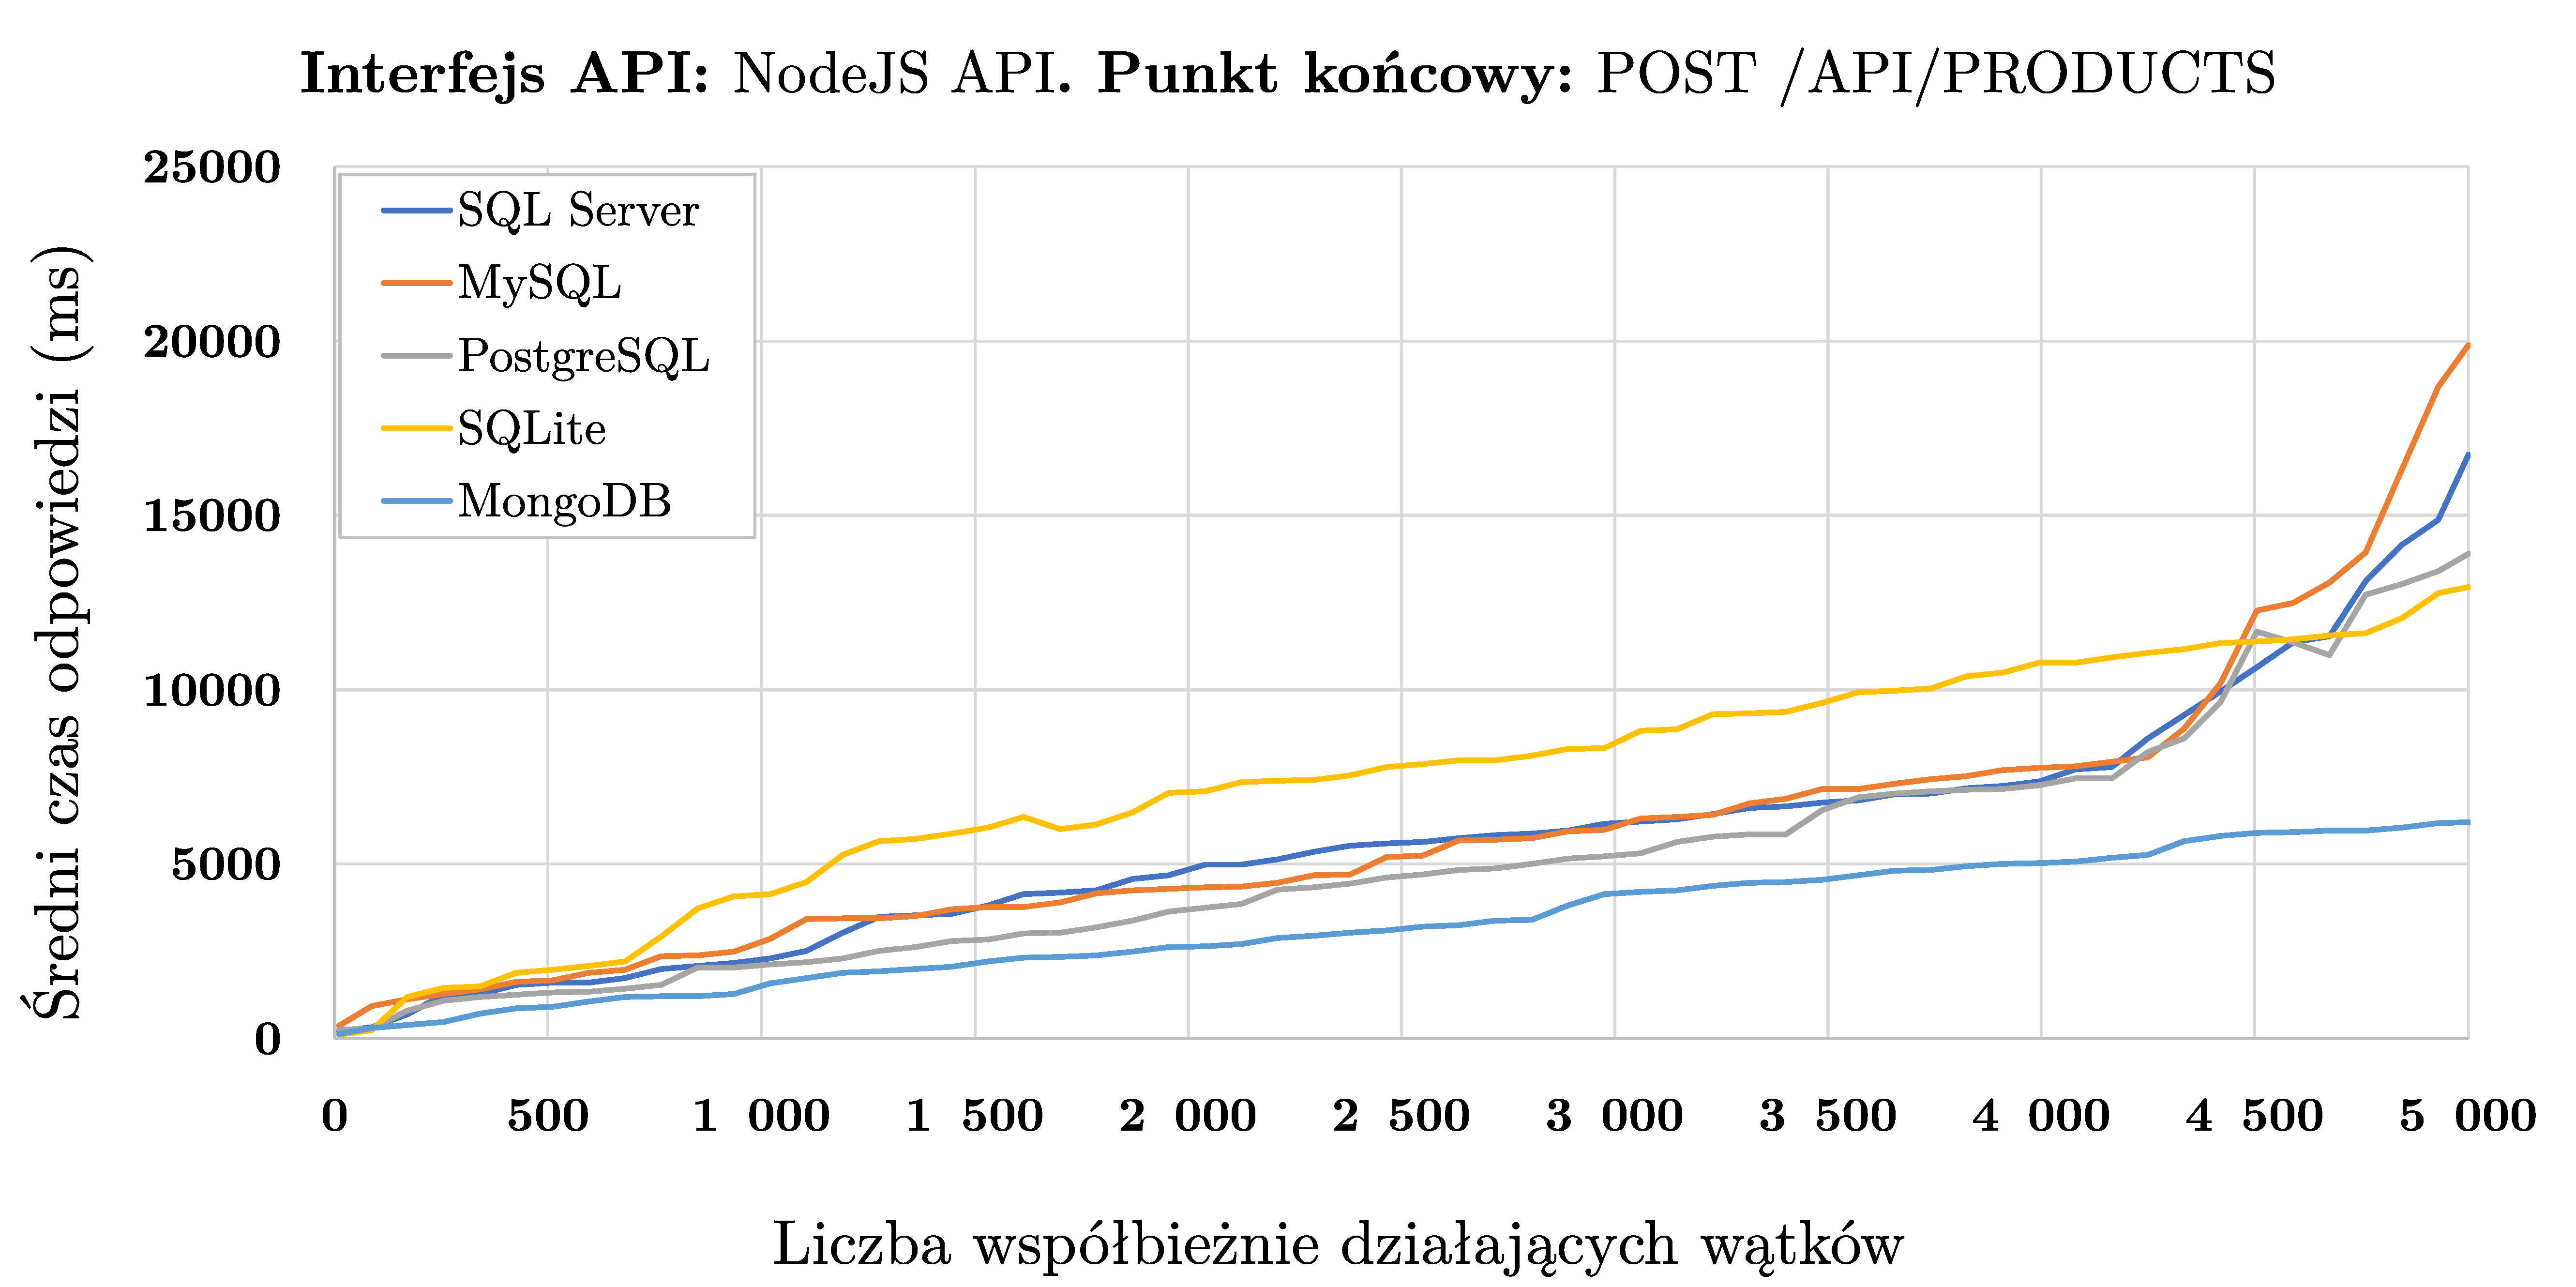
\includegraphics[width=0.49\textwidth]{rys05/response-nodejs-addProduct.pdf} \\
    g) & h) \\
    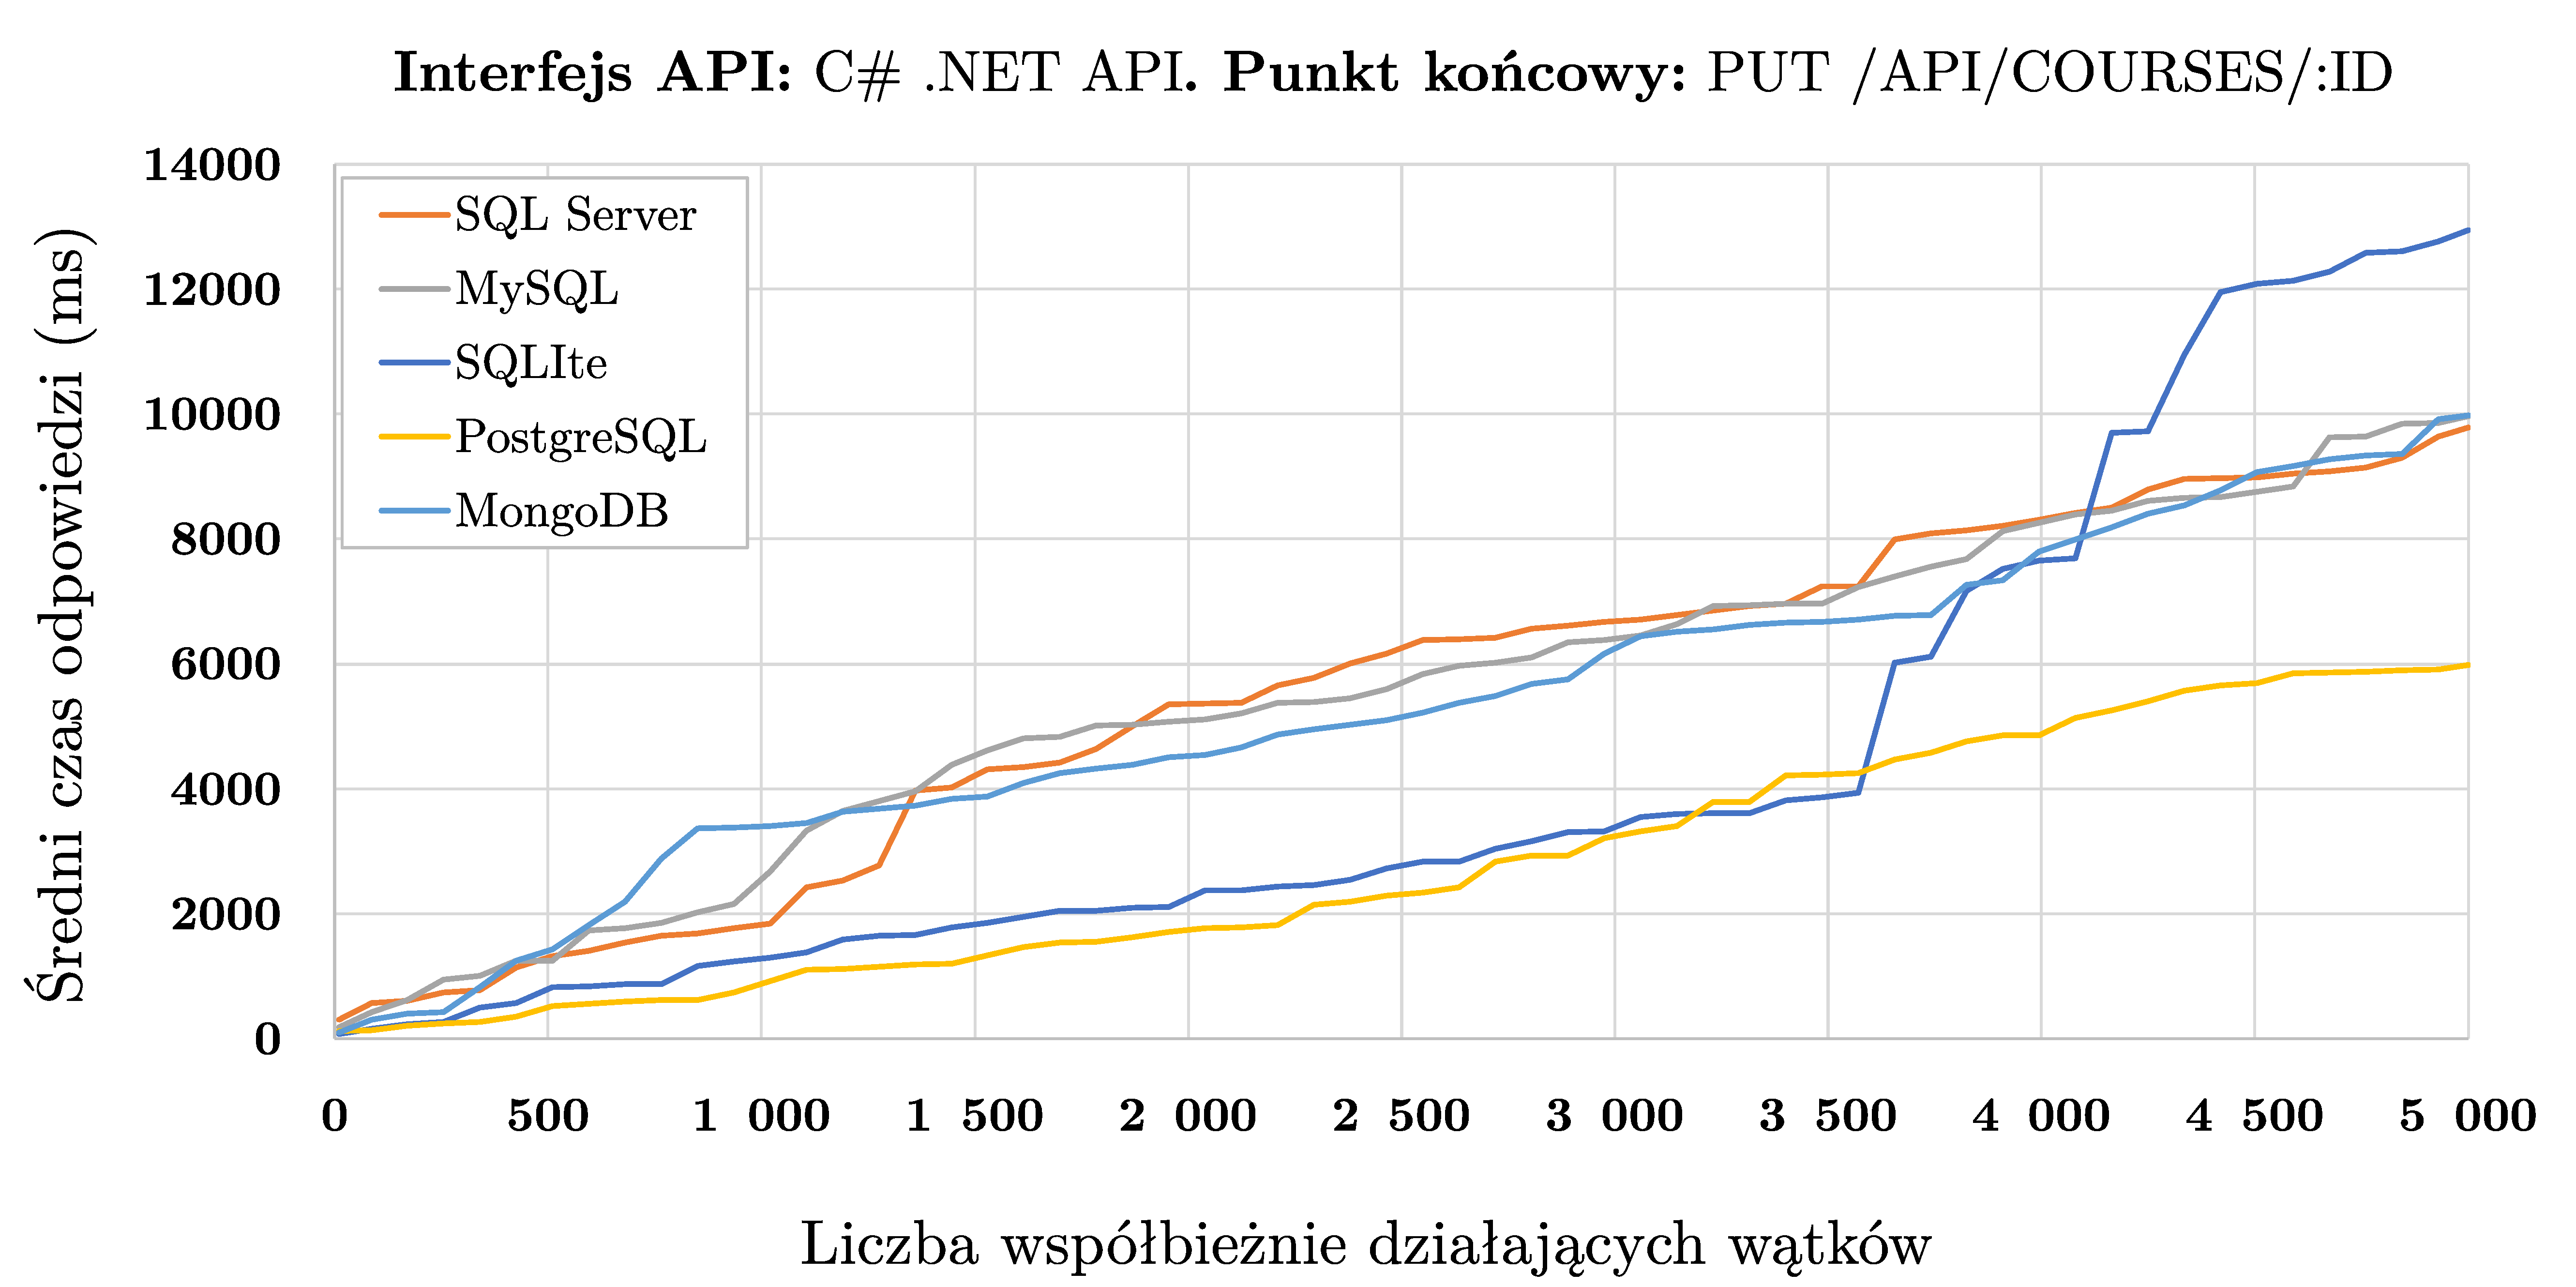
\includegraphics[width=0.49\textwidth]{rys05/response-dotnet-updateCourse.pdf} & 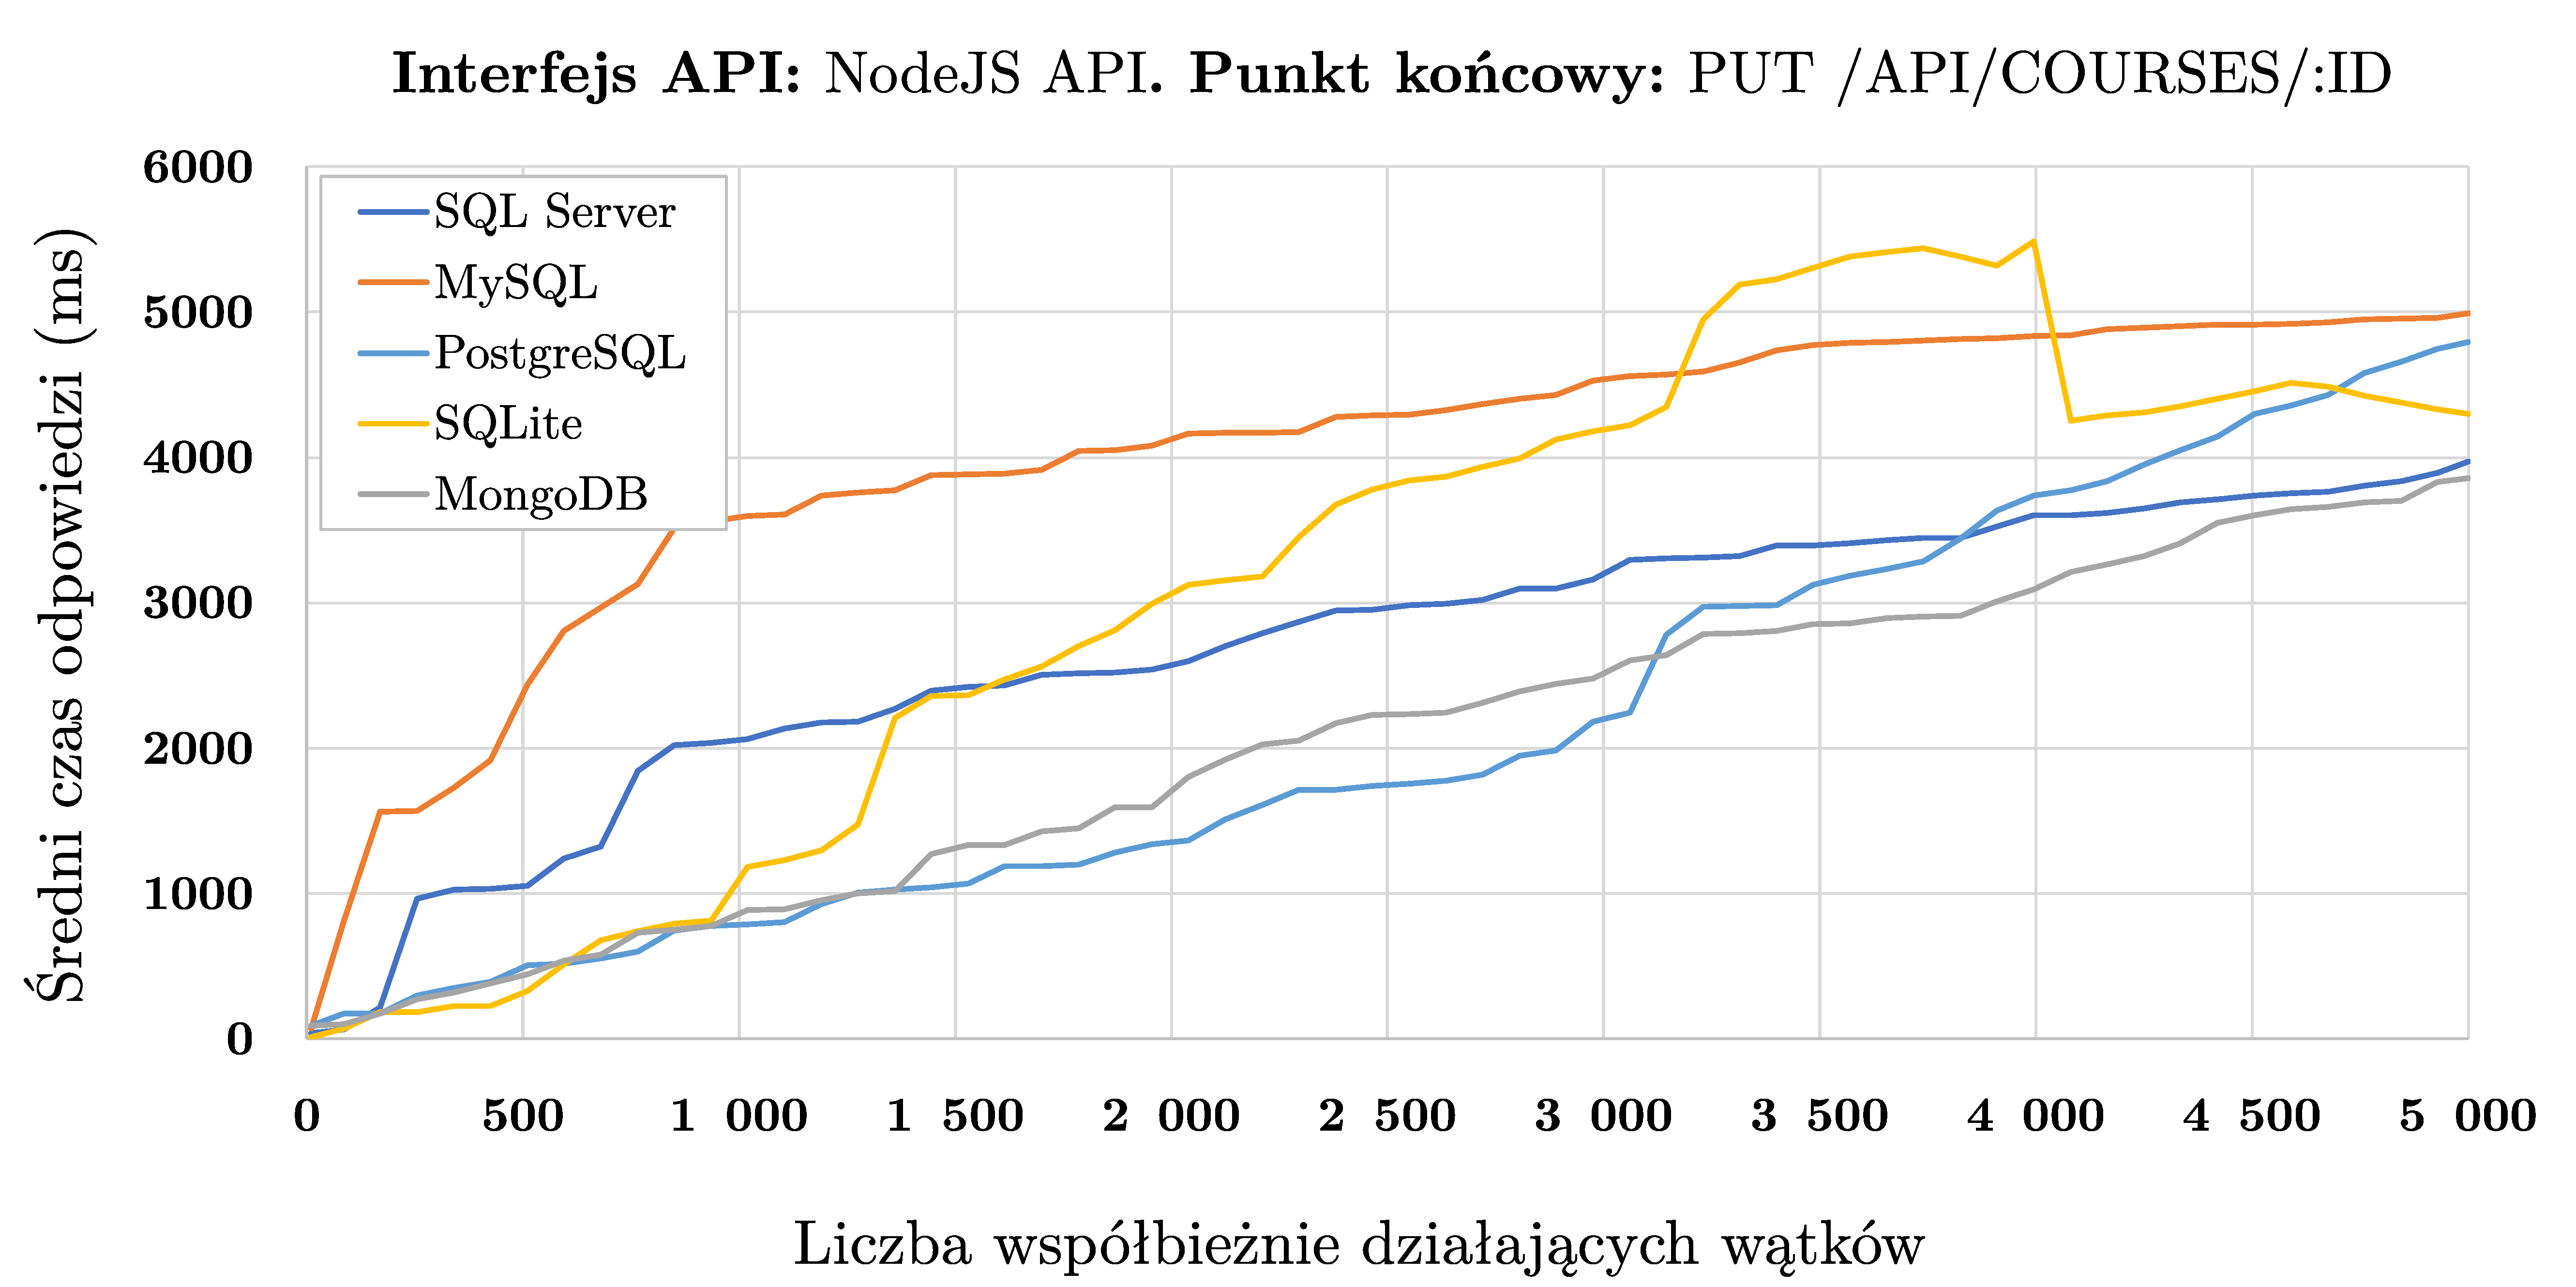
\includegraphics[width=0.49\textwidth]{rys05/response-nodejs-updateCourse.pdf} \\
    i) & j) \\
    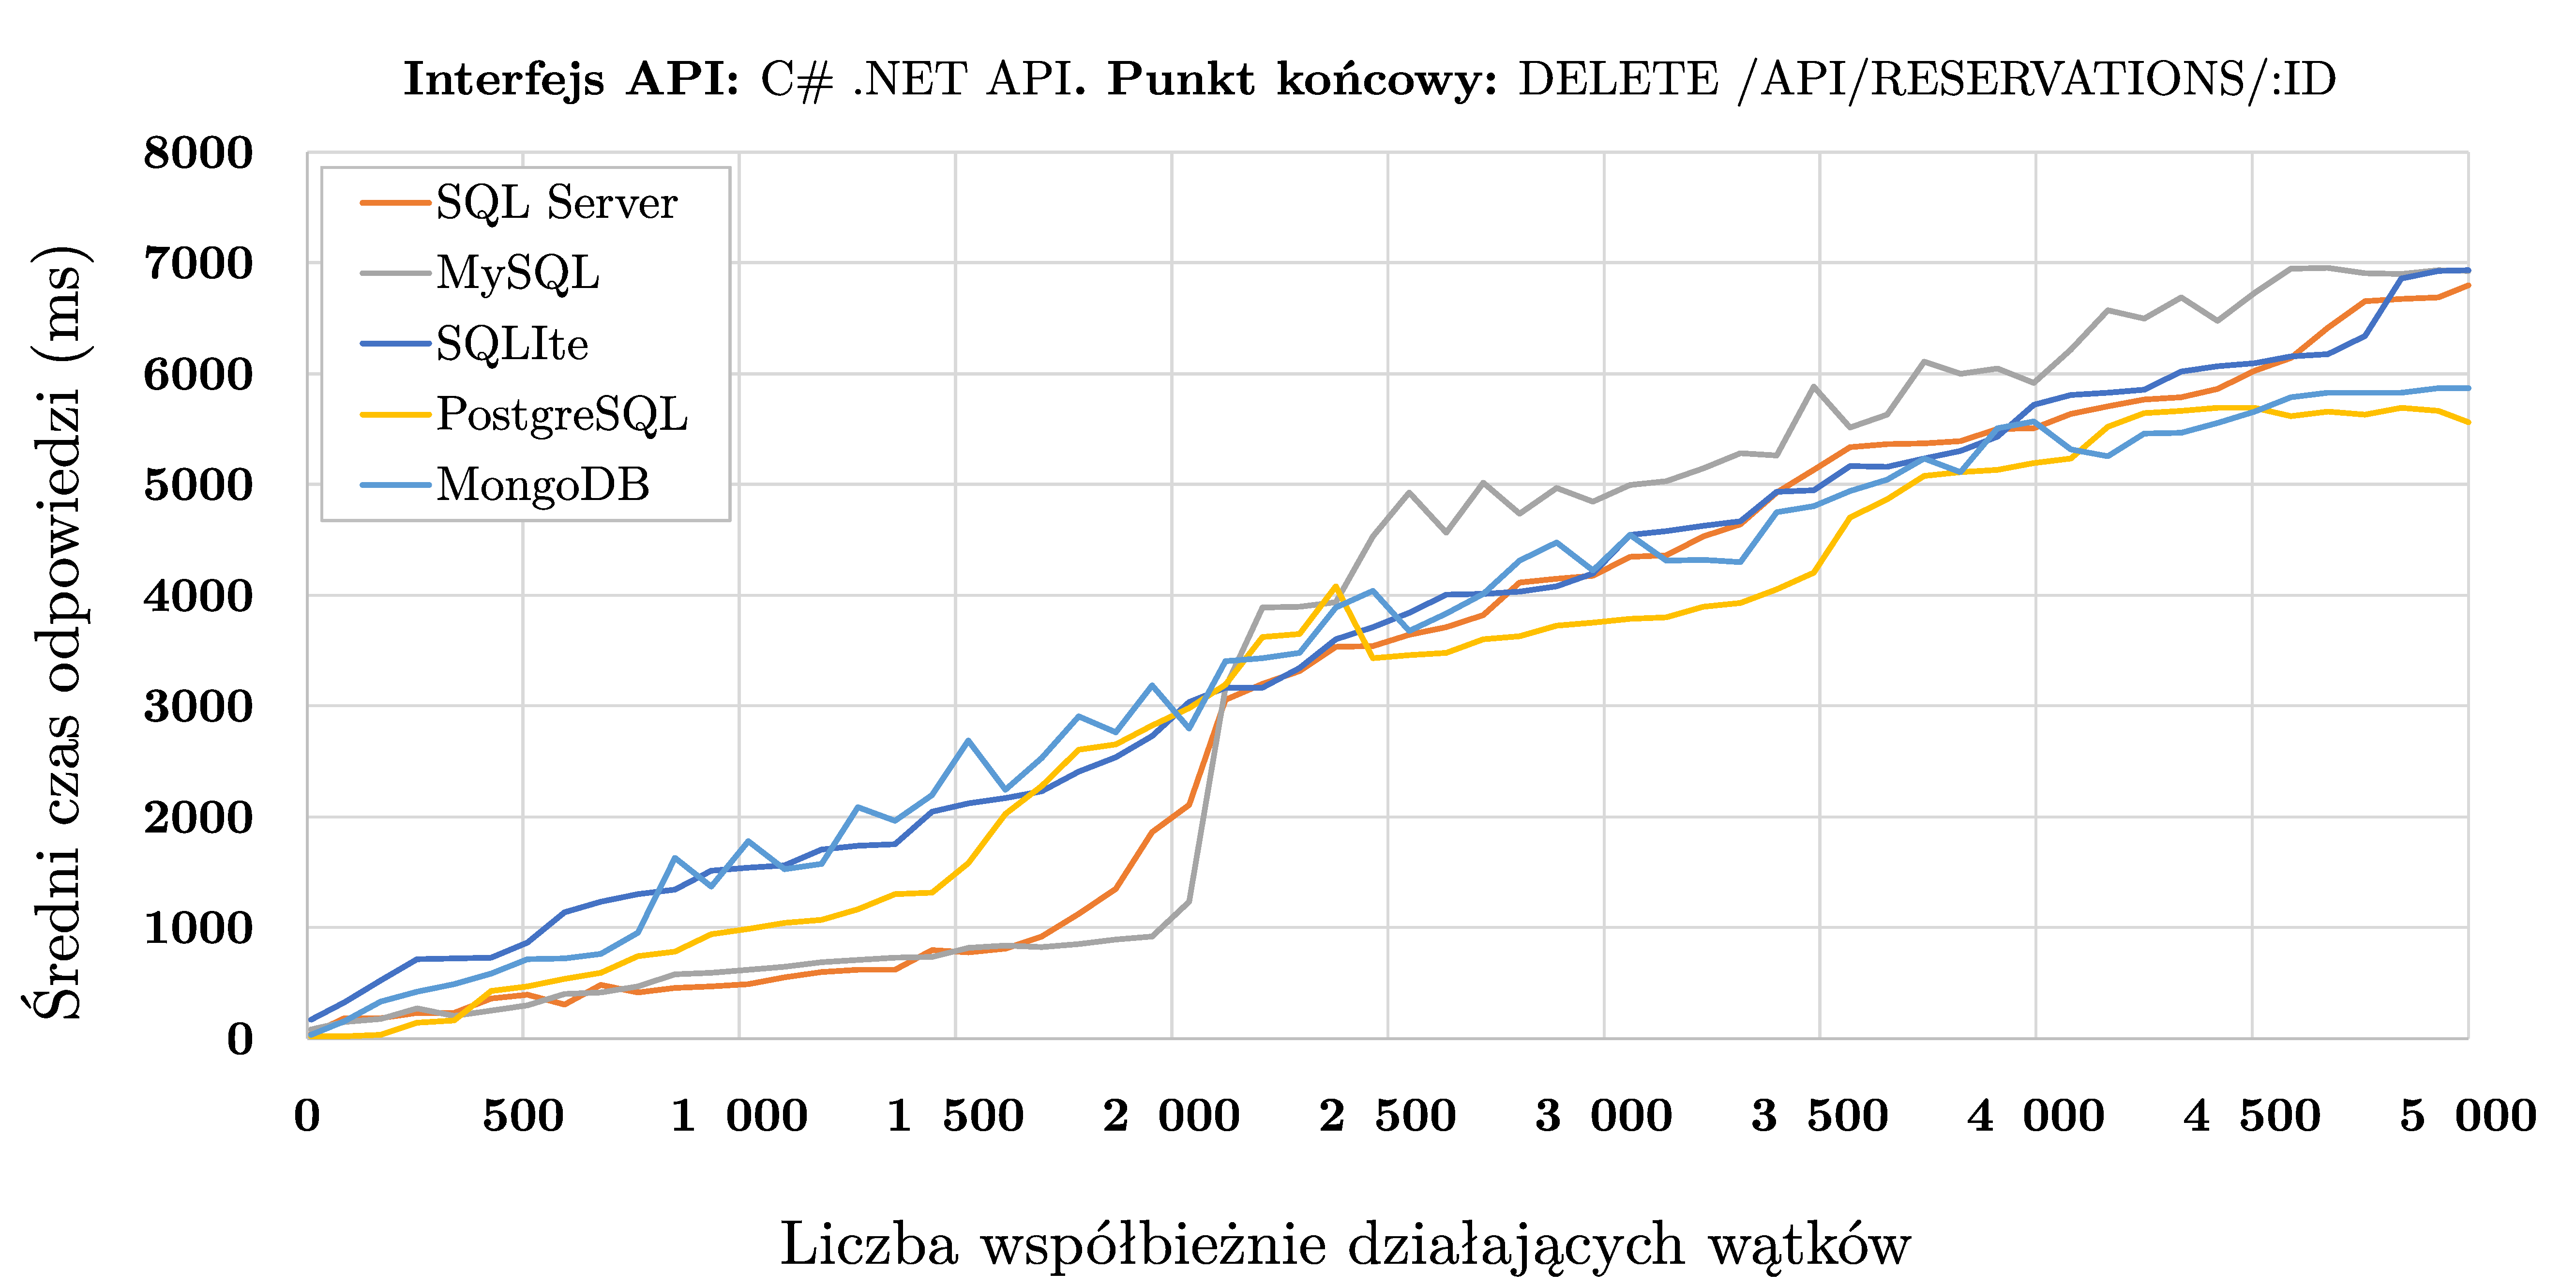
\includegraphics[width=0.49\textwidth]{rys05/response-dotnet-deleteReservation.pdf} & 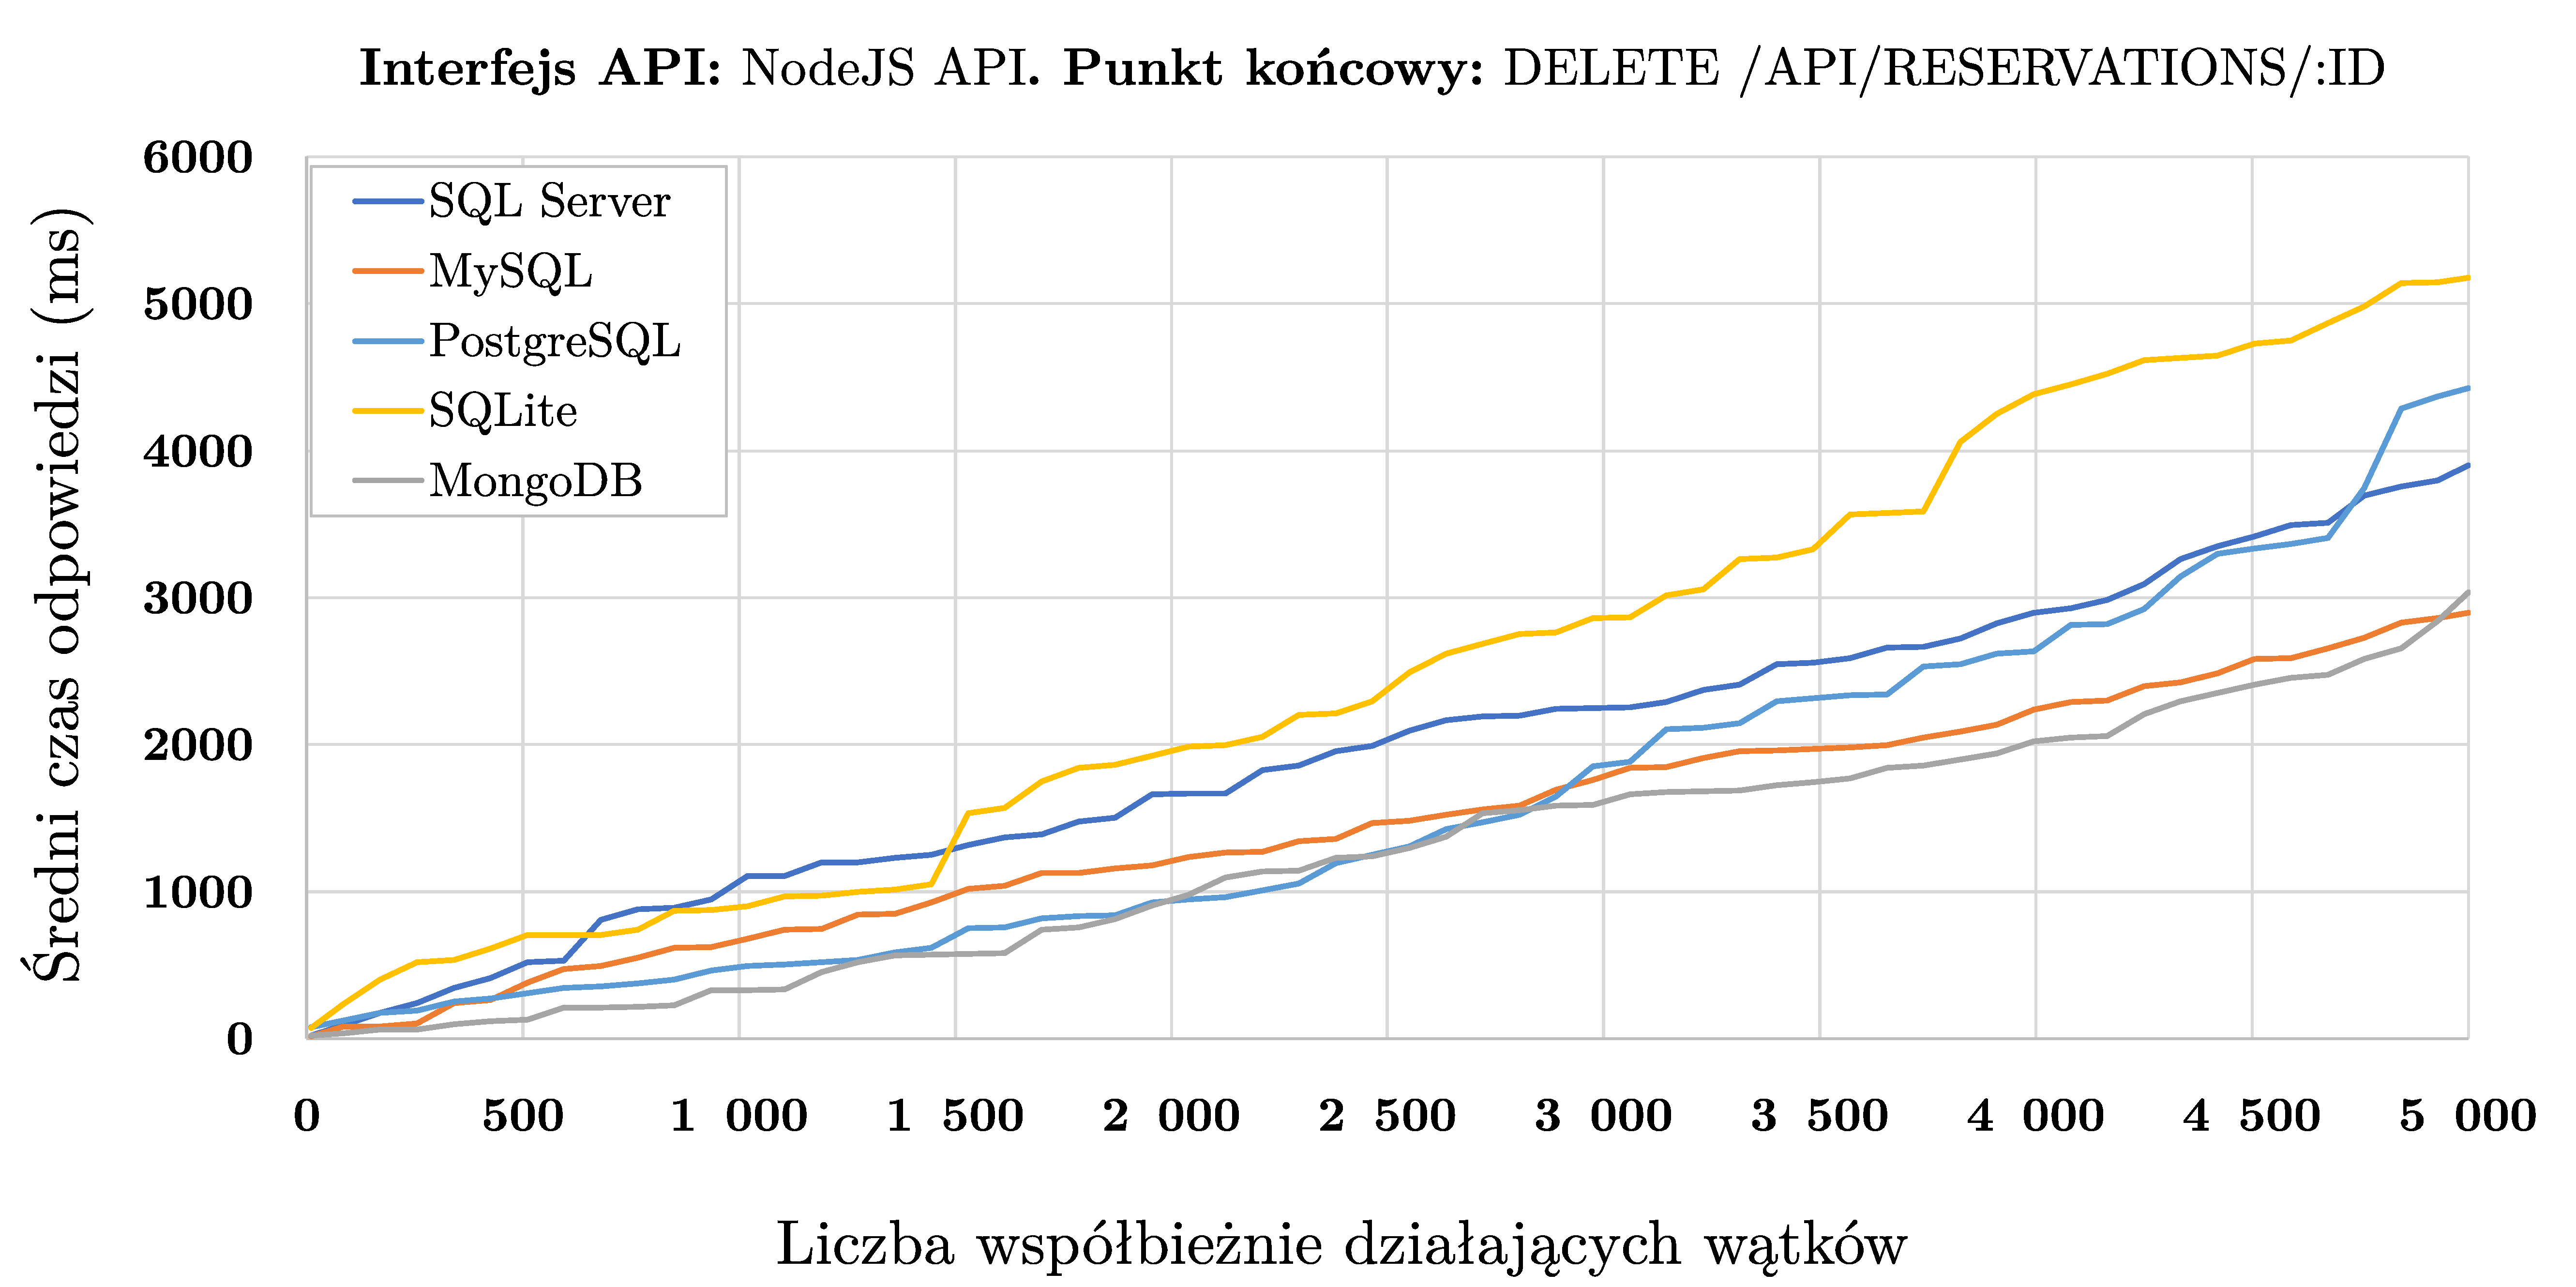
\includegraphics[width=0.49\textwidth]{rys05/response-nodejs-deleteReservation.pdf} \\
	% jezeli obraki sa rownej wysokosci, mozna je wyrownac do gory stosujac vtop jak nizej
	% \vtop{\vskip-2ex\hbox{{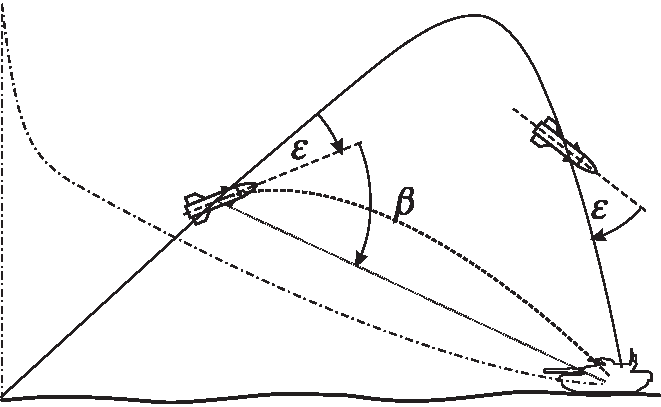
\includegraphics[width=0.475\textwidth]{rys05/beta1}}}} &
	% \vtop{\vskip-2ex\hbox{{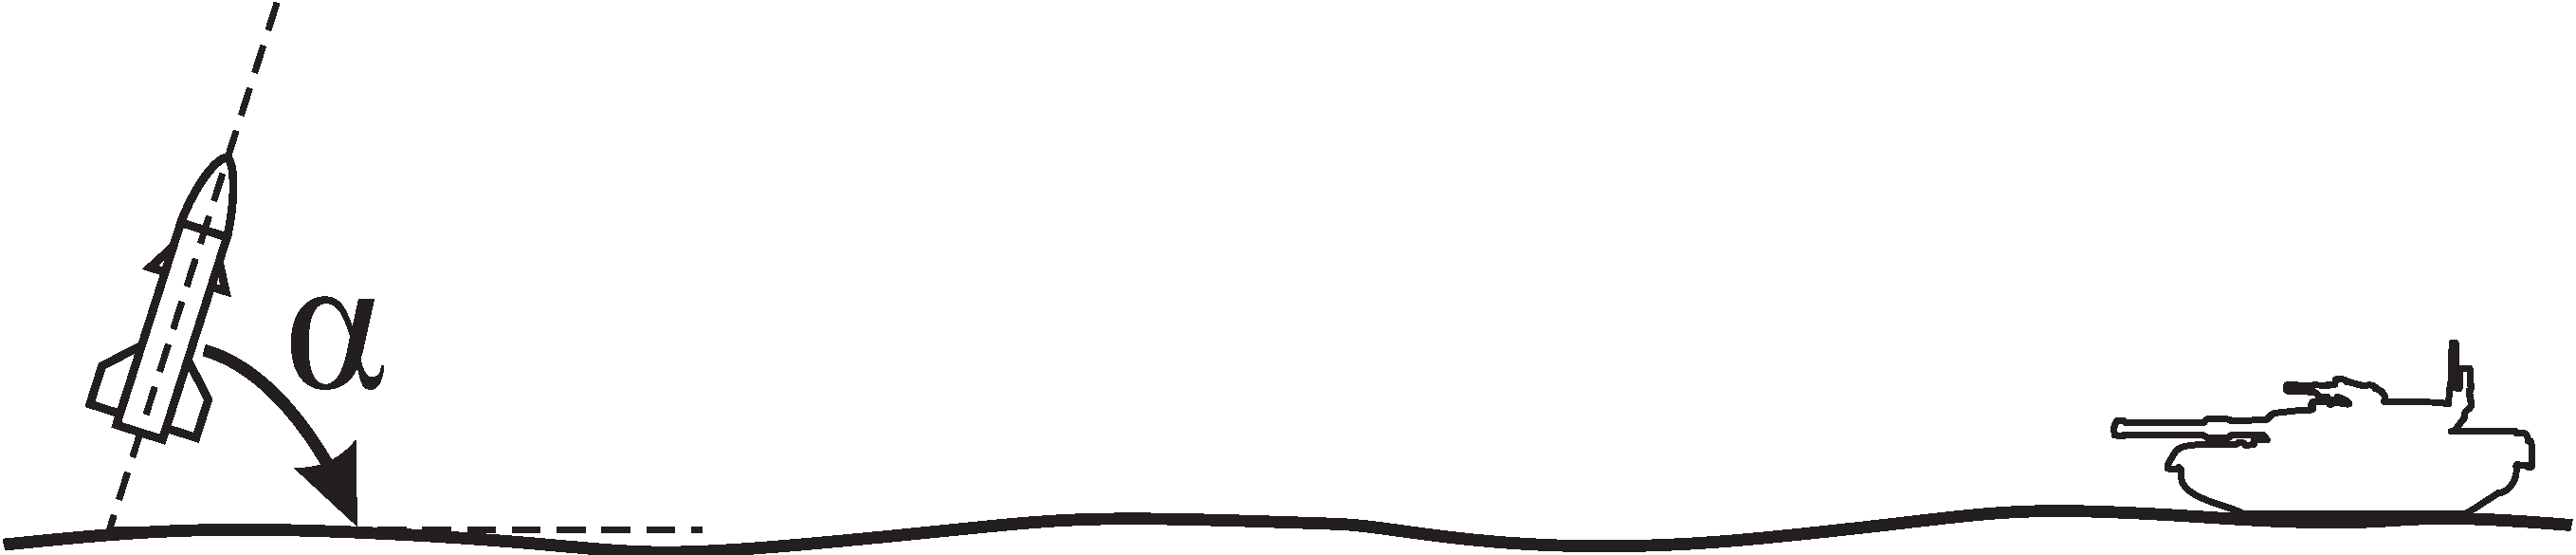
\includegraphics[width=0.475\textwidth]{rys05/alfa1}}}}  \caption{Wyznaczanie trajektorii lotu rakiety: 
	\end{tabular}
  \caption{Średnie czasy odpowiedzi na żądanie względem liczby procesów generujących oraz systemu bazodanowego}
  \label{fig:response-mtc-1}
\end{figure}

Dla tego właśnie przedziału, jedyną zauważalną anomalię dotyczącą zmiany wydajności dostrzec można w kontekście interfejsu programowania aplikacji C\# .NET korzystającego z silnika bazy danych PostgreSQL. W tym przypadku znaczące różnice pomiędzy wydajnością omawianego systemu, a efektywnością drugiego najgorszego rozwiązania odnotowano już dla około \textbf{720} współbieżnie pracujących wątków. Dla tej właśnie metryki, omawiana różnica wynosi \textbf{374 ms}. Wraz ze wzrostem liczby użytkowników o tysiąc, zauważyć możemy różnicę \textbf{759 ms}, a o dwa tysiące - \textbf{2326 ms}. W momencie zaprzestania obserwacji tendencji nieznacznych dysproporcji pomiędzy systemami baz danych (moment ten możemy aproksymować do chwili działania 3750 jednoczesnych procesów-generatorów) dywergencja czasów odpowiedzi osiągnęła wartość \textbf{4855 ms}.

Dysproporcje wskazujące na niezaprzeczalną wyższość określonych rozwiązań nad pozostałymi dostrzegalne są dla rezultatów otrzymywanych w wyniku wspólnej pracy więcej niż czterech tysięcy procesów oprogramowania Apache JMeter. 

Odwołując się do interfejsu zaimplementowanego w technologii NodeJS, zauważyć możemy fakt, że spośród rozwiązań relacyjnych, najniższy skok wartości odnotowały rozwiązania MySQL oraz PostgreSQL. Ponadto, skok ten nastąpił zdecydowanie później, niż miało to miejsce w przypadku pozostałych rozwiązań. Wartym odnotowania są wyniki zaobserwowane dla nierelacyjnego systemu bazodanowego. W przypadku silnika bazy danych MongoDB, średnie czasy odpowiedzi były względnie niskie nie tylko do chwili uruchomienia czterech tysięcy wątków, ale również po tym czasie nie odnotowano gwałtownego wzrostu monitorowanej metryki. W momencie generowania maksymalnego natężenia ruchu sieciowego, zmierzony średni czas odpowiedzi wyniósł \textbf{5846 ms}.

W przypadku rozwiązania zdefiniowanego na bazie technologii Microsoft, zauważalna jest bardzo niska wydajność obsługi komunikacji z rozwiązaniem SQLite (maksymalna zmierzona wartość to \textbf{22515 ms}). Ponadto, silnik bazy danych PostgreSQL, analogicznie do obszaru niższego natężenia ruchu, notuje wyniki gorsze od swoich relacyjnych oraz nierelacyjnych odpowiedników w granicach od \textbf{2111 ms} do \textbf{5373 ms}.

W kontekście pobierania pojedynczego wyniku, wzrosty wartości średniego czasu odpowiedzi posiadają charakterystkę przybliżoną do charakterystyki liniowej. Wyjątkami są tutaj systemy bazy danych MongoDB dla interfejsu napisanego w języku C\#, oraz silnik MySQL dla NodeJS API. W obu przypadkach pojawiają się gwałtowne wzrosty wartości czasu odpowiedzi. Odnosząc się do MongoDB zaobserwować możemy zmianę metryki wydajności od \textbf{1549 ms} do \textbf{5945 ms} na przestrzeni przyrostu wątków od liczby \textbf{3748} do \textbf{4253}. Zmiana ta, utrzymuje się do końca przeprowadzania testu. Dla interfejsu programowania aplikacji uruchamianego w środowisku NodeJS, oraz dla systemu bazodanowego MySQL, anomalia dostrzegana jest dla \textbf{2465} wątków a jej amplituda to \textbf{6721 ms}. Co ciekawe, przekraczając poziom natężenia wynoszący \textbf{2890} wątków, średni czas odpowiedzi zaczyna spadać, aby w punkcie \textbf{4080} stanowić minimum w odniesieniu do pozostałych systemów baz danych.

Poddając pod analizę procedurę zapisu danych do bazy, zgromadzone wyniki wykazują przewagę rozwiązania opartego o język C\#, niezależnie od systemu bazodanowego. Ponadto, liniowa charakterystyka wzrostu metryk dla interfejsu JavaScript zakłócona została pojawieniem się nagłych spadków wydajnościowych. Analogicznie do punktu końcowego pobierania listy obiektów, najmniej znaczący spadek odnotować należy w odniesieniu do nierelacyjnego systemu MongoDB. W tym przypadku zmiana nastąpiła od wartości \textbf{5261 ms} dla \textbf{4247} wątków do wartości \textbf{6203 ms} dla \textbf{5000} wątków.
    
W aspekcie dwóch ostatnich procedur realizowanych przez punkty końcowe interfejsów programowania aplikacji, podobnie jak w przypadku funkcjonalności pozyskiwania pojedynczej encji, zaobserwować możemy przybliżone do liniowych, zmiany monitorowanego parametru wydajności. Spośród interesujących anomalii zaobserwowanych w ramach czterech ostatnich wykresów wyróżnić należy spadek wydajnościowy silnika bazodanowego SQLite w przypadku modyfikacji encji za pomocą interfejsu API .NET. Spadek ten, identyfikowany jest poprzez wzrost średniego czasu odpowiedzi o \textbf{8018 ms}, w przedziale czasowym w którym uruchomiono dodatkowe \textbf{847} wątków. Niestandardowym zachowaniem cechują się również systemy bazodanowe SQL Server oraz MySQL w odniesieniu do operacji usuwania pojedynczego rekordu poprzez API implementowane w języku C\#. Interfejsy korzystające z obu mechanizmów przechowywania danych, do momentu osiągnięcia odpowiednio \textbf{1725} oraz \textbf{1955} współbieżnie pracujących wątków generowania żądań, cechowały się wyjątkowo niskim średnim czasem odpowiedzi (tj. odpowiednio \textbf{827 ms} oraz \textbf{922 ms}).

Podsumowując, zarówno wskazanie wyższości jednej z technologii niezależnie od systemów baz danych, jak i wyróżnienie pojedynczego systemu bazy danych w kontekście realizowanej operacji nie jest możliwe biorąc pod uwagę kształt przeprowadzonego badania. Możliwym jest jednak zaobserowanie niskiego poziomu kompatybilności pomiędzy interfejsem API napisanym w języku C\# oraz systemem baz danych SQLite. Ponadto, relatywnie wysoką wydajnością względem innych rozwiązań bazodanowych cechuje się system nierelacyjny MongoDB. W pięciu na dziesięć porównaniach wydajnościowych, przedstawionych na omawianych wykresach, to właśnie ten silnik baz danych najdłużej utrzymuje najniższą wartość średniego czasu odpowiedzi względem pozostałych rozwiązań.

Przedstawione powyżej wyniki nie dostarczają jednakże pełnego obrazu faktycznej wydajności ewaluowanych usług. Należy pamiętać, że uzyskana odpowiedź na żądanie nie musi być zawsze pozytywna, przez co nie zawsze niesie ona ze sobą informacje pożądaną dla klienta. Na wykresach \ref{fig:response-with-errors} a) oraz \ref{fig:response-with-errors} b) zestawiono ze sobą informacje o średnim czasie odpowiedzi na żądanie, a także o procencie żądań zakończonych niepomyślnie. Poprzez niepomyślne zakończenie żądania, rozumiano zarówno uzyskanie odpowiedzi o niepoprawnym kodzie i treści ciała, jak i zgłoszenie wyjątku protokołu hipertekstowego związanego z odmową aplikacji względem realizacji zapytania. Choć zobrazowano tu tylko i wyłącznie przypadek pojedynczej operacji oraz jednego systemu bazodanowego, analogiczne zachowanie zaobserwować można dla wszystkich pozostałych operacji i jest ono specyficzne dla interfejsu programowania aplikacji. 

\begin{figure}[htb]
    \centering
      \begin{tabular}{@{}ll@{}}
      a) & b) \\
      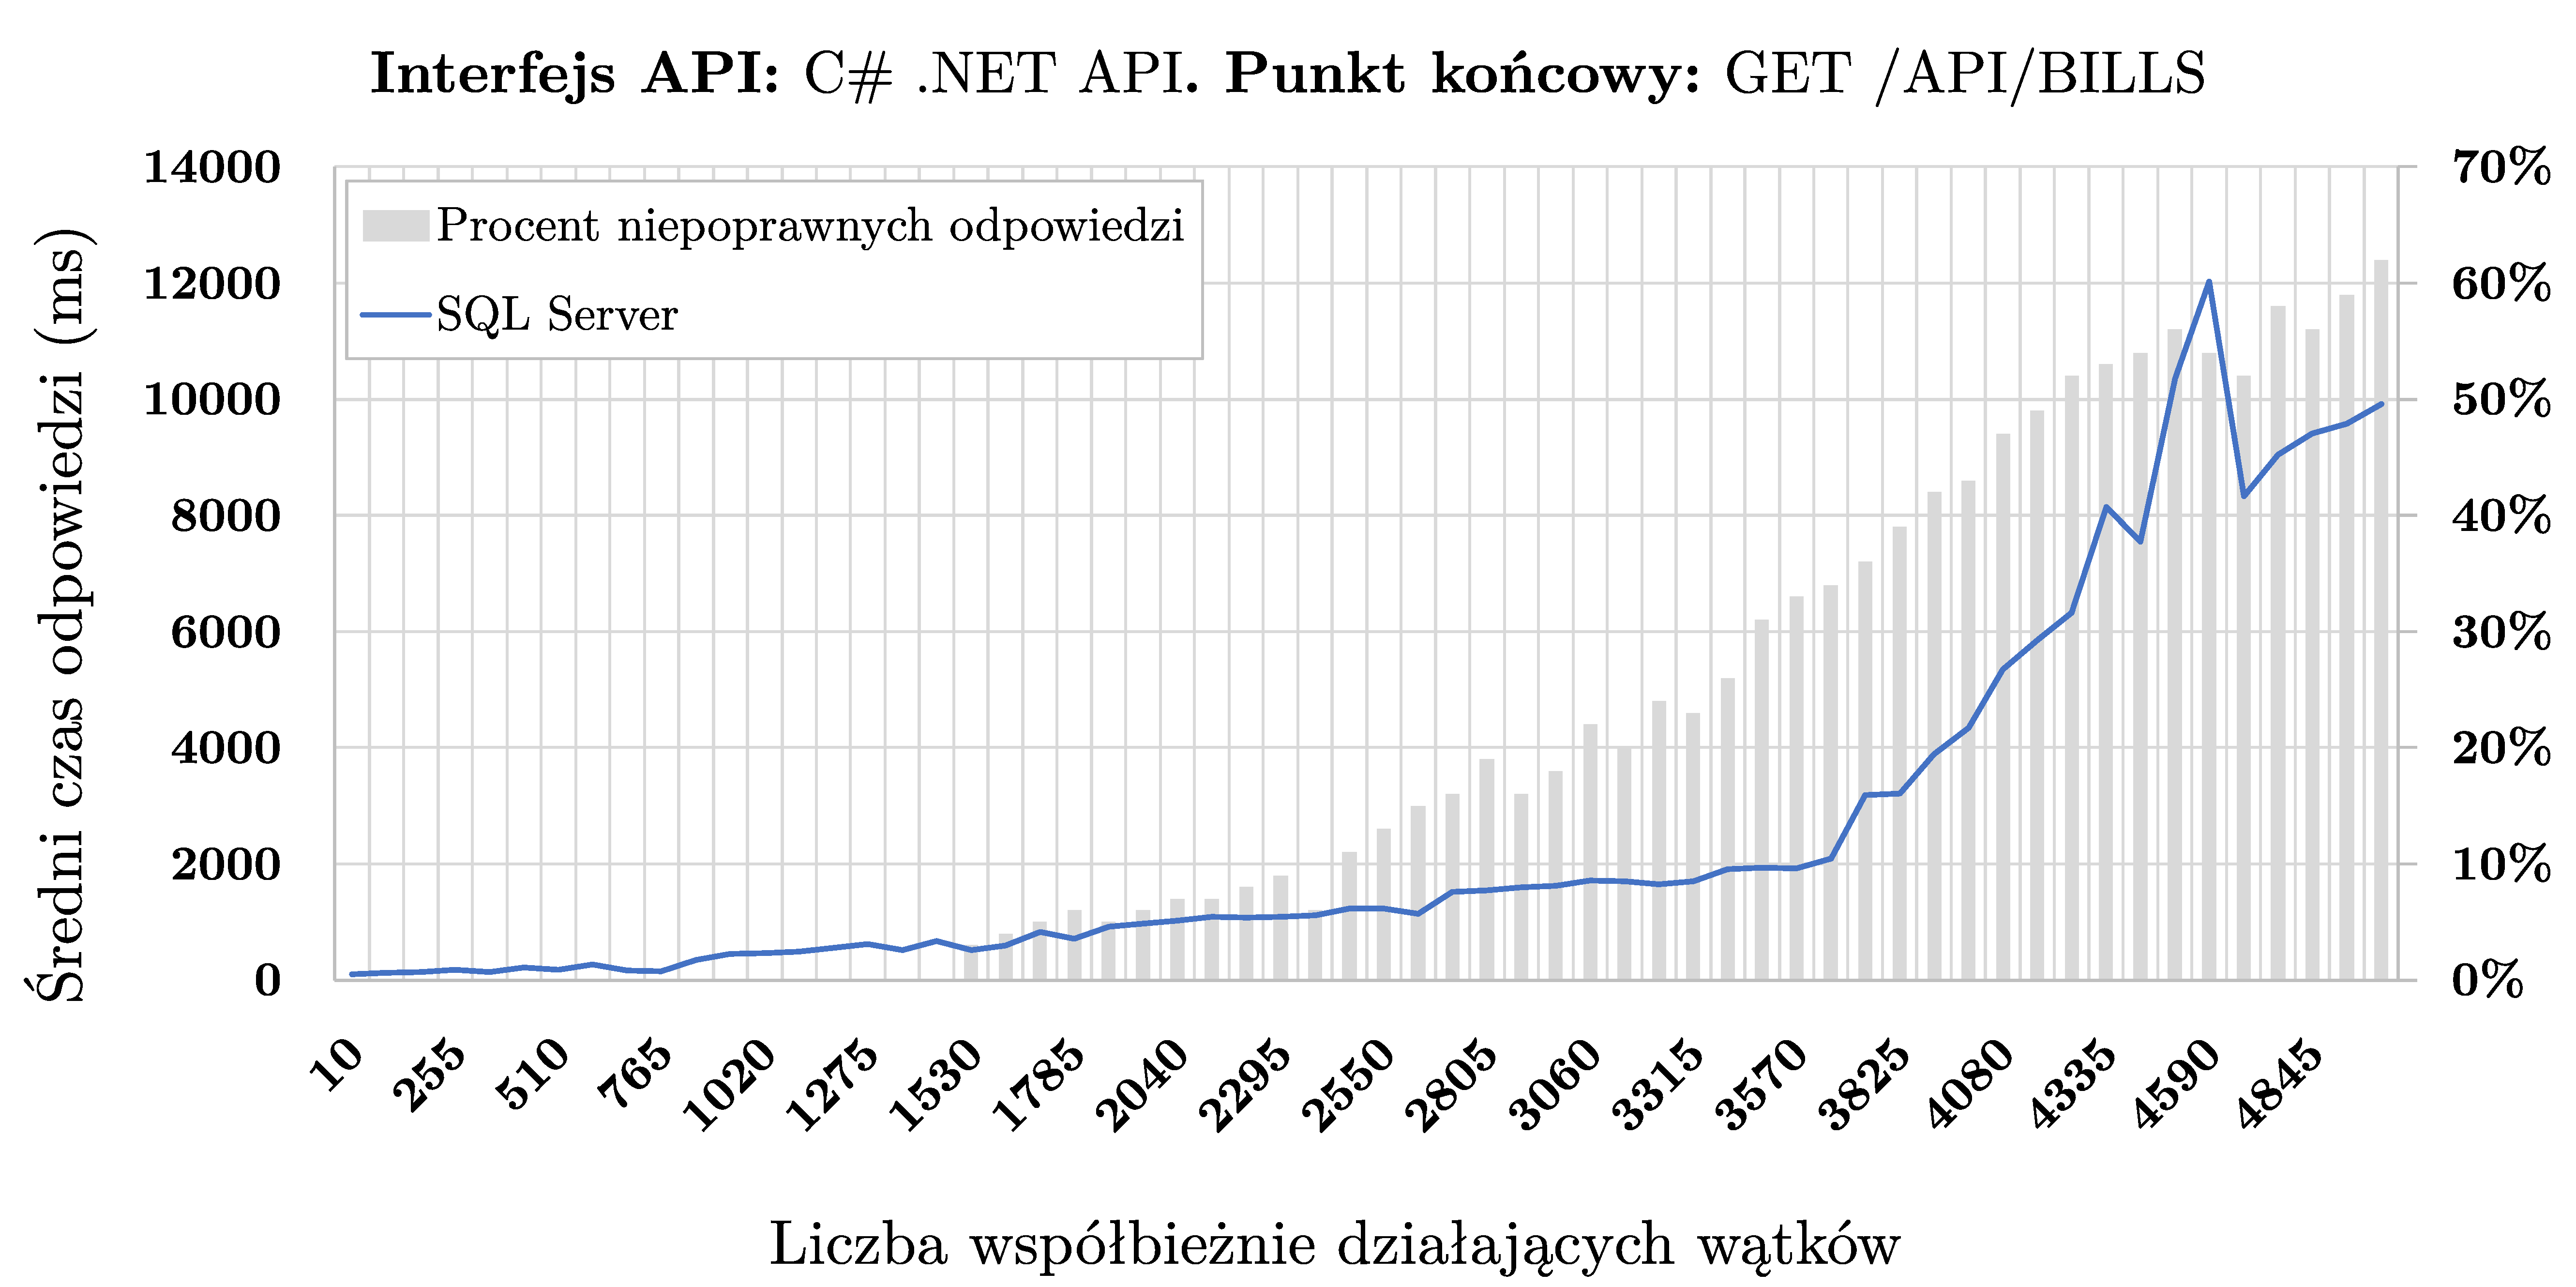
\includegraphics[width=0.49\textwidth]{rys05/response-and-errors-dotnet.pdf} & 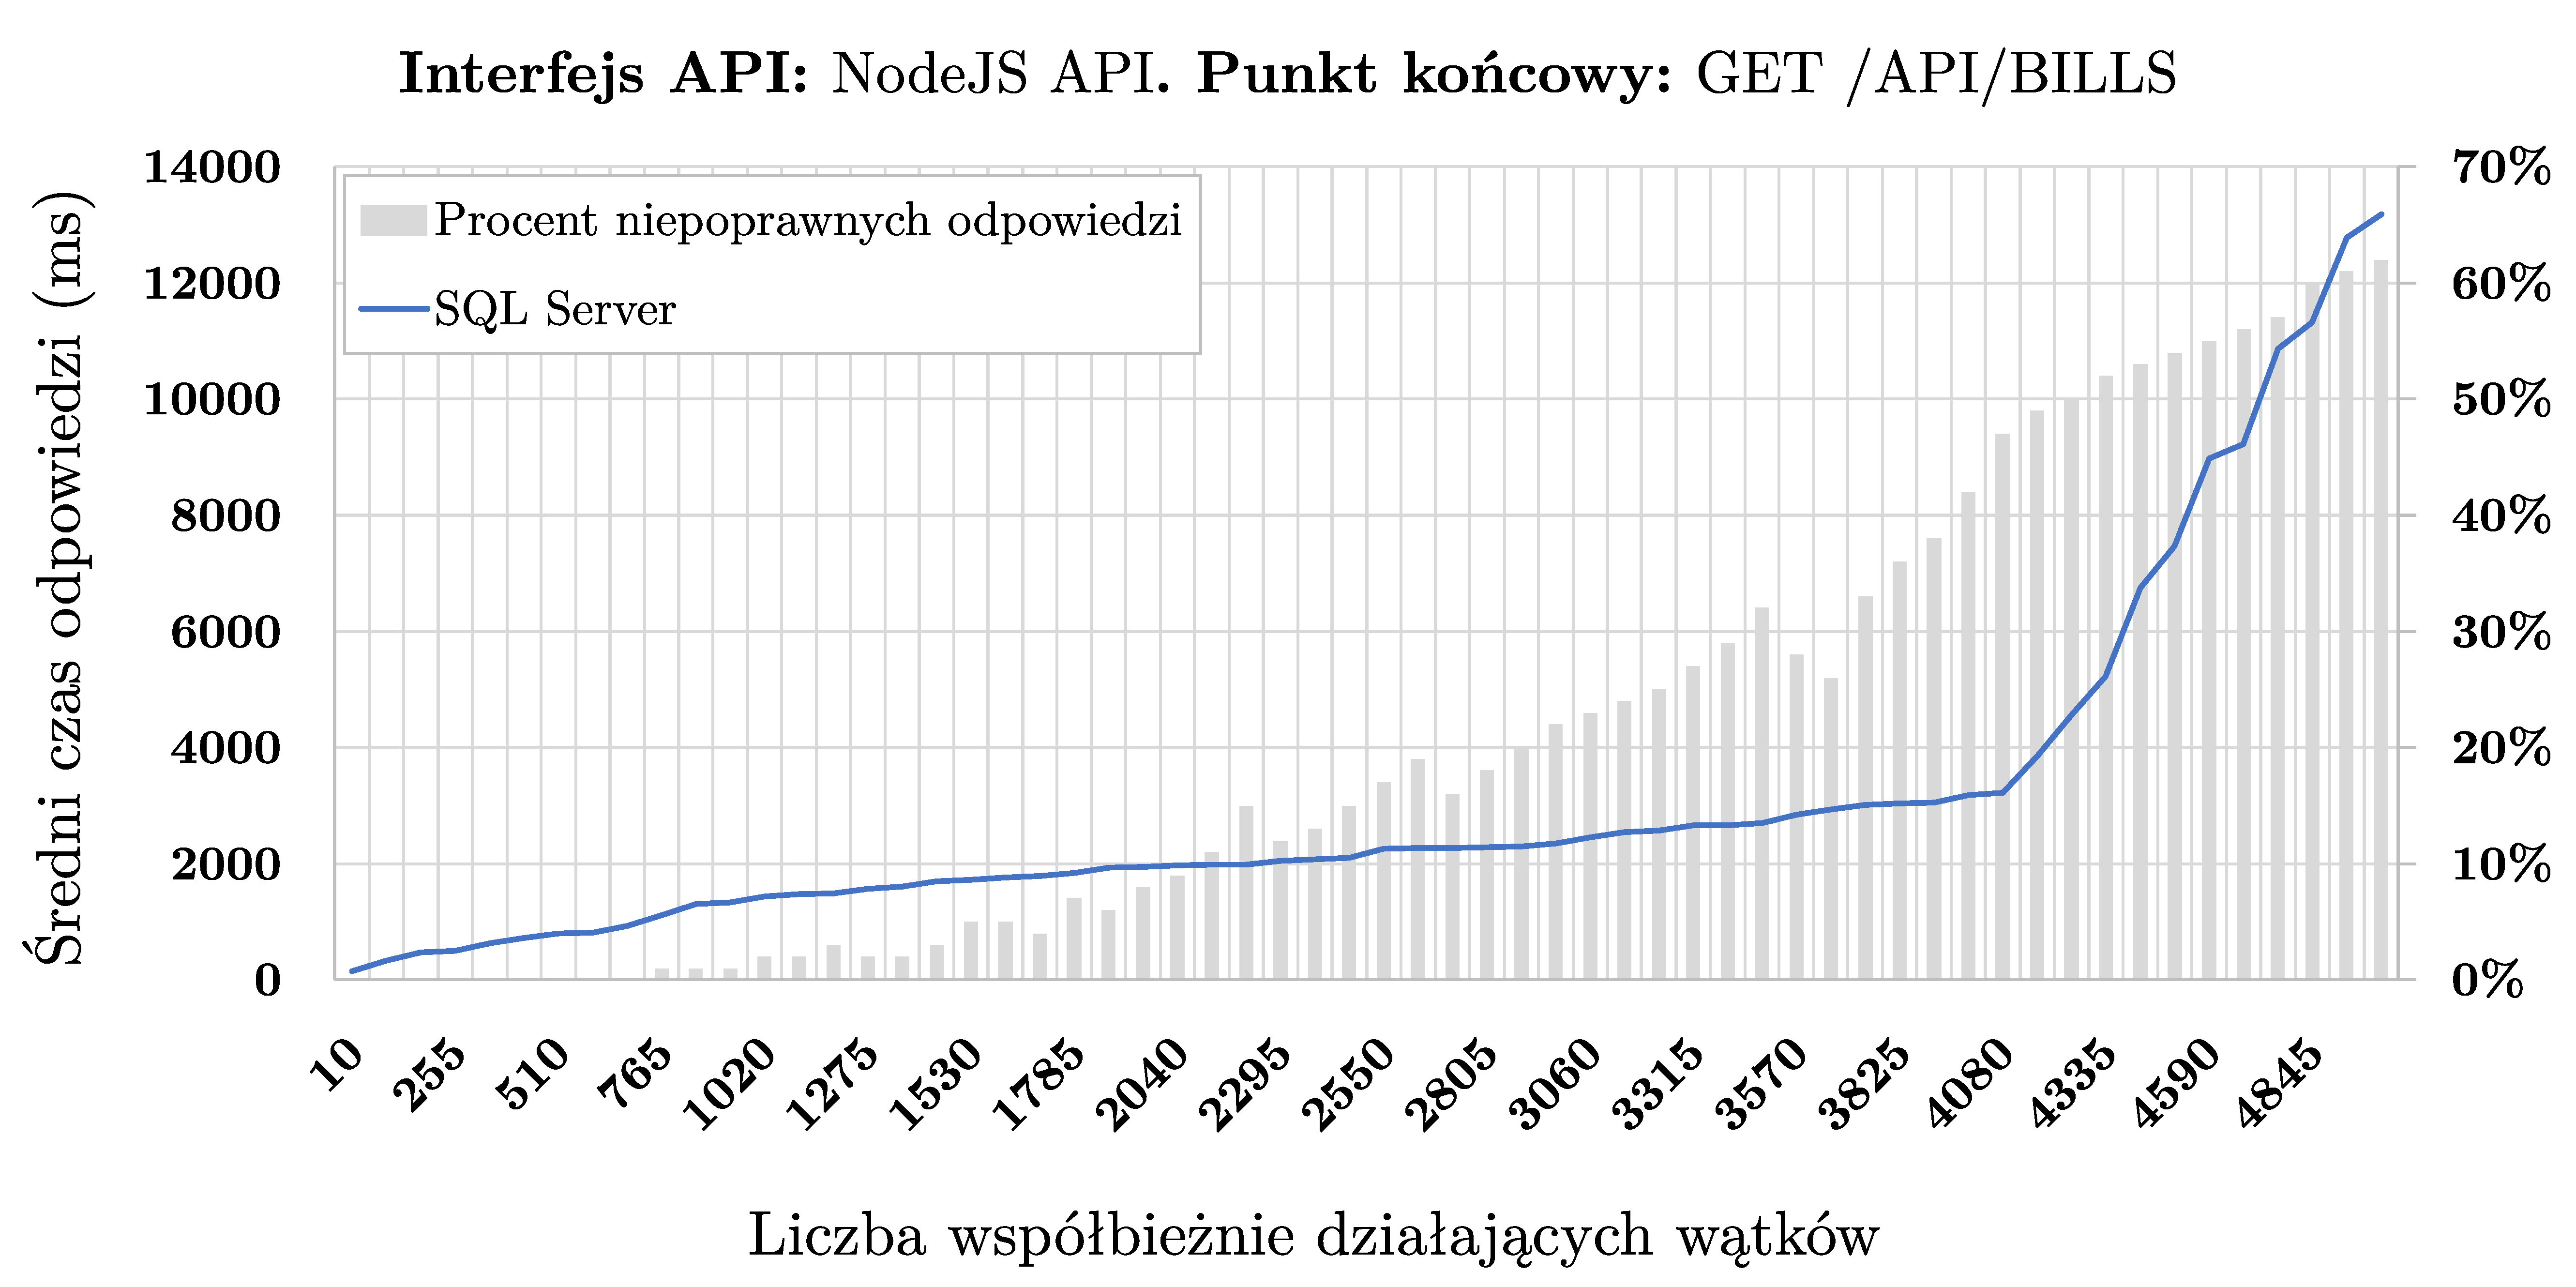
\includegraphics[width=0.49\textwidth]{rys05/response-and-errors-nodejs.pdf}
      % jezeli obraki sa rownej wysokosci, mozna je wyrownac do gory stosujac vtop jak nizej
      % \vtop{\vskip-2ex\hbox{{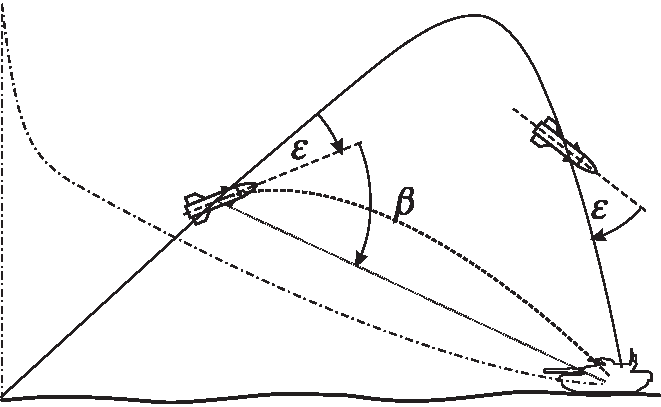
\includegraphics[width=0.475\textwidth]{rys05/beta1}}}} &
      % \vtop{\vskip-2ex\hbox{{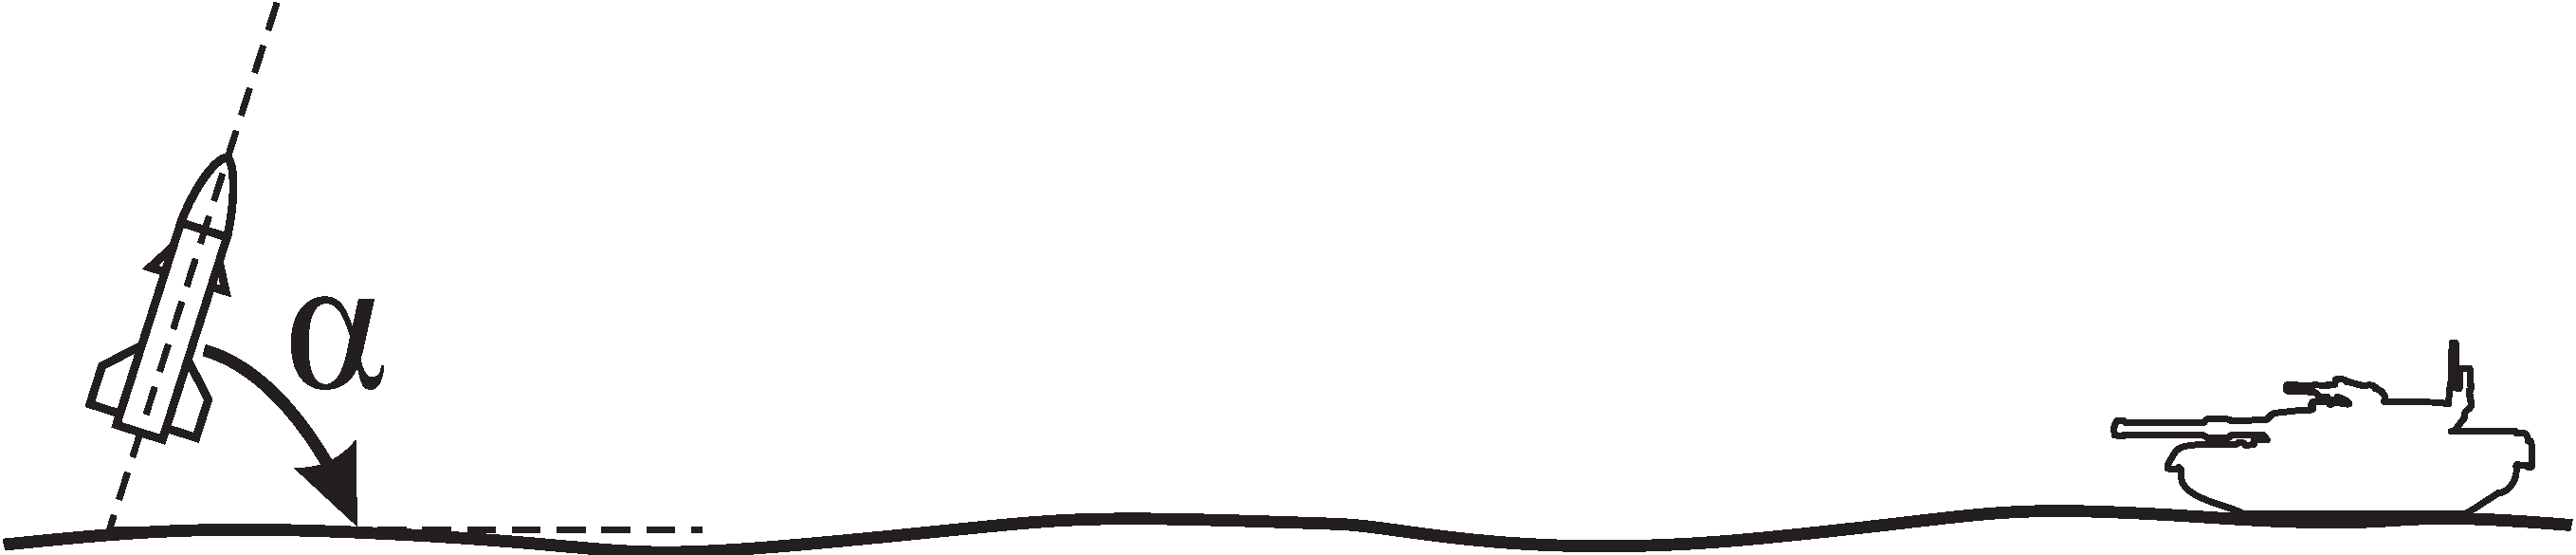
\includegraphics[width=0.475\textwidth]{rys05/alfa1}}}}  \caption{Wyznaczanie trajektorii lotu rakiety: 
      \end{tabular}
    \caption{Średnie czasy odpowiedzi na żądanie oraz procent niepoprawnych odpowiedzi względem liczby procesów generujących}
    \label{fig:response-with-errors}
  \end{figure}

Analizując przedstawione wykresy należy zwrócić uwagę zarówno na moment pojawiania się błędów obsługi żądania, jak i na stopień korelacji błędów z czasem przetwarzania zapytania. W przypadku interfejsu API opartego o technologię .NET widzimy, że procent błędów jest silnie powiązany ze zwiększającym się przedziałem czasowym obsługi komendy, a także intensyfikacją ruchu sieciowego. Oznacza to, że serwer w momencie kolejkowania żądań do przetworzenia, nie bierze pod uwagę ich liczby i stara się przetwarzać każde, jakie do niego dotrze. W związku z odmową realizacji funkcjonalności ze strony API, serwer zgłasza wyjątek protokołu hipertekstowego. Z racji konieczności wykonania pracy w kontekście każdego żądania, niezależnie od niewielkiego prawdopodobieństwa jego pomyślnej realizacji, wydłuża się czas uzyskania odpowiedzi na zapytanie klienckie.

Odnosząc się do interfejsu zaimplementowanego w technologii NodeJS, zaobserwować możemy odmienne zachowanie. Pierwszym aspektem na jaki należy zwrócić uwagę jest pojawienie się błędów obsługi żądania zdecydowanie wcześniej (tj. przy znacząco mniejszej liczbie uruchomionych wątków testowych). Oznacza to, że usługa nie jest w stanie radzić sobie na tyle dobrze z dostarczanym ruchem, jak robi to interfejs napisany w języku C\#. Jednakże, wraz z rosnącym błędem procentowym nie zmienia się czas obsługi żądania. Oznacza to, że komponent serwerowy w ramach API nie przetwarza każdego z zapytań jakie zostanie do niego dostarczone, a także to, że w pewien specyficzny względem swojej charakterystyki sposób, API dokonuje wyboru tych spośród otrzymanych żądań, które mają zostać natychmiastowo odrzucone. Taki model przetwarzania komunikatów pozwala na utrzymanie niskiego poziomu czasu odpowiedzi, jednakże należy wziąć pod uwagę fakt, że nie musi być ona jednoznaczna z poziomem wydajności działania API.
\section{Wpływ zastosowanej technologii na wydajność realizacji operacji współbieżnych}
Niniejsze badanie, przeprowadzone zostało w celu zaobserwowania różnic dotyczących sposobu przetwarzania długo trwających operacji. Potencjalnie różnice te, związane mogą być z odmienną implementacją wewnętrznych mechanizmów przetwarzania współbieżnego, a także diametralnie innym podejściem obu technologii do zagadnienia wielowątkowości. Zdecydowano się na implementację algorytmu rozwiązującego symetryczny problem komiwojażera, bazującego na metaheurystyce genetycznej. Elementy charakterystyczne względem omawianego rozwiązania przedstawiono w sekcji \ref{label:algorytm-genetyczny}. Napisane programy, zawarte są wewnątrz warstwy logiki biznesowej interfejsów API, a punktem wprowadzania danych dla algorytmów są określone punkty końcowe. W odniesieniu do przekazywanych danych wejściowych, wyróżnić należy ciało żądania, zawierające tablicę obiektów notacji JSON. Obiekty te, identyfikują określone lokalizacje poprzez wprowadzenie parametrów długości oraz szerokości geograficznej. Ponadto, przekazywany zostaje parametr czasu trwania głównej pętli algorytmu (tj. jak długo program powinien dokonywać kalkulacji), a także wartość wyniku optymalnego, względem której program powinien porównać uzyskany rezultat.

Odnosząc się do protokołu badawczego, zdecydowano się na wykonanie pomiarów jakości uzyskanego rozwiązania, a także liczby iteracji głównej pętli implementowanego algorytmu. Metryki te, zostały zebrane w kontekście uruchomienia programu dla pietnastu odmiennych zbiorów danych testowych, dostępnych w ramach otwartej biblioteki TSPLib \cite{TSPLIB_ARTICLE}. Dla każdego ze zbiorów danych, trzydziestokrotnie powtórzono wywołanie algorytmu, w obrębie każdego z czterech różnych czasów wykonywania iteracji głównej programu. Czasy te to: 15s, 30s, 45s oraz 60s. W momencie przeprowadzenia badania, a także przez cały okres jego trwania, uruchomionych było 30 współbieżnie pracujących wątków będących generatorami żądań.

Przed rozpoczęciem realizacji omówionego protokołu przeprowadzono ewaluację funkcjonalną, stanowiącą warunek początkowy podjęcia badań. Ewaluacja ta, polegała na pięciokrotnym odwołaniu się punktów końcowych api obu technologii, wprowadzając jako dane wejściowe, zbiory współrzędnych dostępnych w ramach biblioteki TSPLib. Warto zaznaczyć, że są to zbiory inne, niż te wykorzystane następnie w faktycznym badaniu. Kryterium akceptacji warunku początkowego, było pomyślne wykonanie algorytmu w każdym ze zdefiniowanych przypadków funkcjonalnych, a także zwrócenie poprawnej odpowiedzi w czasie zgodnym z parametrem czasu wykonania alogytmu. Oba wymienione kryteria zostały w czasie ewaluacji funkcjonalnej spełnione.

Następnie, przygotowano lokalną topologię fizyczną nr 2, której schemat zaprezentowany został w sekcji \ref{sec:lokalne-srodowisko-badawcze-ver-2} oraz rozpoczęto generowanie żądań. Już na tym etapie, a jeszcze przed otrzymaniem wyników działania algorytmu, zaobserwowano interesujące zachowanie dotyczące obsługi długo trwających żądań. Analizując czasy rozpoczęcia oraz zakończenia pracy dla poszczególnych wątków Apache JMeter, a także całkowity czas trwania badania dla każdego z interfejsów programowania aplikacji, dostrzeżono pełną sekwencyjność przetwarzania zapytań w przypadku API zaimplementowanego w technologii JavaScript / NodeJS, a także częściowe zrównoleglenie operacji w kontekście technologii C\# .NET. W konsekwencji tego, ewaluacja usługi sieciowej opartej o NodeJS trwała 18 godzin i 52 minuty, podczas gdy badanie interfejsu napisanego w języku programowania C\# -- 5 godzin i 27 minut. Tak znacząca dysproporcja wynika ze sposobu zarządzania wykonaniem zapytań poprzez zastosowanie podejścia wielowątkowości, a także pracy z wykorzystaniem pojedynczego wątku.

Kiedy żądanie zacznie być przetwarzane przez interfejs programowania aplikacji NodeJS, jest ono wykonywane do momentu: uzyskania wyniku, przekroczenia dozwolonego czasu realizacji zapytania \textit{(ang. timeout)}, bądź też przekazania tokenu przerwania \textit{(ang. cancellation token)}. Jeżeli w czasie obsługi żądania pojawi się następne, musi ono zostać przekazane do kolejki, po to, aby stać się aktywnym po zakończeniu przetwarzania poprzedniej wiadomości.

Analizując wewnętrzne mechanizmy usługi sieciowej implementowanej w języku C\# zauważyć możemy odmienne, niż zaprezentowane powyżej podejście. W związku z faktem utworzenia nowego wątku dla głównej pętli algorytmu, wątek podstawowy programu nie jest obciążony koniecznością realizacji jakichkolwiek dodatkowych operacji i oczekuje na uzyskanie wyników z procesu potomnego. Jeżeli w czasie oczekiwania pojawi się przychodzące żądanie, wątek główny zapisuje kontekst wywołania dla obecnego zapytania, przechodzi do realizacji kolejnego z nich, a po jego zakończeniu, bądź w momencie wyczekiwania na zakończenie, przełącza się do kontekstu poprzedniego zadania, aby zweryfikować jego status. Dzięki zastosowaniu takiego podejścia, które możliwe jest tylko w sytuacji dostępności wielu wątków w ramach pojedynczego programu, usługa sieciowa nie jest blokowana względem innych klientów.

Po ukończeniu obsługi wszystkich wygenerowanych żądań, przez oba systemy internetowe, uśredniono serie każdych 30 rezultatów, uzyskanych względem różnych zbiorów testowych oraz odmiennych czasów wykonania. Opracowane wyniki, przedstawiono w tabelach \ref{tab:mtc-2} oraz \ref{tab:mtc-2-2}.

\begin{table}[ht]
  \centering
  \caption{Wydajność realizacji algorytmu genetycznego dla problemu komiwojażera w zależności od czasu przetwarzania oraz technologii -- współczynnik jakości rozwiązania}
  \label{tab:mtc-2}
  \resizebox{\columnwidth}{!}{%
  \begin{tabular}{|l|llll|llll|}
  \hline
  \multicolumn{1}{|c|}{\multirow{2}{*}{}} &
    \multicolumn{4}{c|}{C\# / .NET} &
    \multicolumn{4}{c|}{JavaScript / NodeJS} \\ \cline{2-9} 
  \multicolumn{1}{|c|}{} &
    \multicolumn{1}{c|}{15s} &
    \multicolumn{1}{c|}{30s} &
    \multicolumn{1}{c|}{45s} &
    \multicolumn{1}{c|}{60s} &
    \multicolumn{1}{c|}{15s} &
    \multicolumn{1}{c|}{30s} &
    \multicolumn{1}{c|}{45s} &
    \multicolumn{1}{c|}{60s} \\ \hline\hline
  burma14 &
    \multicolumn{1}{l|}{0,3462 } &
    \multicolumn{1}{l|}{\textbf{0,6847}} &
    \multicolumn{1}{l|}{0,8475 } &
    \textbf{0,8589} &
    \multicolumn{1}{l|}{0,2983 } &
    \multicolumn{1}{l|}{\textbf{0,5943}} &
    \multicolumn{1}{l|}{0,7636 } &
    0,7579  \\ \hline
  ulysses16 &
    \multicolumn{1}{l|}{0,5299} &
    \multicolumn{1}{l|}{0,3910 } &
    \multicolumn{1}{l|}{0,9270 } &
    0,6549  &
    \multicolumn{1}{l|}{0,4817 } &
    \multicolumn{1}{l|}{0,2857 } &
    \multicolumn{1}{l|}{0,8297 } &
    0,5354  \\ \hline
  ulysses22 &
    \multicolumn{1}{l|}{0,5271 } &
    \multicolumn{1}{l|}{0,4171 } &
    \multicolumn{1}{l|}{0,9312 } &
    0,7824  &
    \multicolumn{1}{l|}{\textbf{0,5488} } &
    \multicolumn{1}{l|}{0,4668 } &
    \multicolumn{1}{l|}{0,8728 } &
    0,6717  \\ \hline
  att48 &
    \multicolumn{1}{l|}{0,0493 } &
    \multicolumn{1}{l|}{0,0611 } &
    \multicolumn{1}{l|}{0,3129 } &
    0,2623  &
    \multicolumn{1}{l|}{0,0242 } &
    \multicolumn{1}{l|}{0,0238 } &
    \multicolumn{1}{l|}{0,2413 } &
    0,2903  \\ \hline
  berlin52 &
    \multicolumn{1}{l|}{0,2316 } &
    \multicolumn{1}{l|}{0,2484 } &
    \multicolumn{1}{l|}{\textbf{0,9718}} &
    0,8398  &
    \multicolumn{1}{l|}{0,2239 } &
    \multicolumn{1}{l|}{0,3861 } &
    \multicolumn{1}{l|}{\textbf{0,9202} } &
    0,7642  \\ \hline
  gr96 &
    \multicolumn{1}{l|}{0,4798 } &
    \multicolumn{1}{l|}{0,1617 } &
    \multicolumn{1}{l|}{0,9274 } &
    0,7808  &
    \multicolumn{1}{l|}{0,4874 } &
    \multicolumn{1}{l|}{0,1386 } &
    \multicolumn{1}{l|}{0,8606 } &
    0,7103  \\ \hline
  bier127 &
    \multicolumn{1}{l|}{0,2313 } &
    \multicolumn{1}{l|}{0,1963 } &
    \multicolumn{1}{l|}{0,8473 } &
    0,8505  &
    \multicolumn{1}{l|}{0,1162 } &
    \multicolumn{1}{l|}{0,1928 } &
    \multicolumn{1}{l|}{0,7906 } &
    0,7792  \\ \hline
  ch130 &
    \multicolumn{1}{l|}{0,0947 } &
    \multicolumn{1}{l|}{0,1328 } &
    \multicolumn{1}{l|}{0,8072 } &
    0,8066  &
    \multicolumn{1}{l|}{0,0575 } &
    \multicolumn{1}{l|}{0,1457 } &
    \multicolumn{1}{l|}{0,7521 } &
    0,6828  \\ \hline
  ch150 &
    \multicolumn{1}{l|}{0,0784 } &
    \multicolumn{1}{l|}{0,1140 } &
    \multicolumn{1}{l|}{0,8584 } &
    0,7966  &
    \multicolumn{1}{l|}{0,0812 } &
    \multicolumn{1}{l|}{0,1483 } &
    \multicolumn{1}{l|}{0,7900 } &
    \textbf{0,7991 } \\ \hline
  tsp225 &
    \multicolumn{1}{l|}{0,2819 } &
    \multicolumn{1}{l|}{0,0988 } &
    \multicolumn{1}{l|}{0,7801 } &
    0,8311  &
    \multicolumn{1}{l|}{0,3057 } &
    \multicolumn{1}{l|}{0,0826 } &
    \multicolumn{1}{l|}{0,8209 } &
    0,7533  \\ \hline
  att532 &
    \multicolumn{1}{l|}{0,0194 } &
    \multicolumn{1}{l|}{0,0171 } &
    \multicolumn{1}{l|}{0,2226 } &
    0,2470  &
    \multicolumn{1}{l|}{0,0116 } &
    \multicolumn{1}{l|}{0,0233 } &
    \multicolumn{1}{l|}{0,2650 } &
    0,1498  \\ \hline
  u574 &
    \multicolumn{1}{l|}{\textbf{0,5940}} &
    \multicolumn{1}{l|}{0,5454 } &
    \multicolumn{1}{l|}{0,6460 } &
    0,7872  &
    \multicolumn{1}{l|}{0,4821 } &
    \multicolumn{1}{l|}{0,3782 } &
    \multicolumn{1}{l|}{0,5836 } &
    0,6573  \\ \hline
  u724 &
    \multicolumn{1}{l|}{0,1620 } &
    \multicolumn{1}{l|}{0,0483 } &
    \multicolumn{1}{l|}{0,6529 } &
    0,7718  &
    \multicolumn{1}{l|}{0,0943 } &
    \multicolumn{1}{l|}{0,0472 } &
    \multicolumn{1}{l|}{0,5747 } &
    0,6369  \\ \hline
  vm1084 &
    \multicolumn{1}{l|}{0,0289 } &
    \multicolumn{1}{l|}{0,0273 } &
    \multicolumn{1}{l|}{0,5971 } &
    0,7938  &
    \multicolumn{1}{l|}{0,0051 } &
    \multicolumn{1}{l|}{0,0381 } &
    \multicolumn{1}{l|}{0,5126 } &
    0,7962  \\ \hline
  d1291 &
    \multicolumn{1}{l|}{0,1927 } &
    \multicolumn{1}{l|}{0,2930 } &
    \multicolumn{1}{l|}{0,5711 } &
    0,8421  &
    \multicolumn{1}{l|}{0,1768 } &
    \multicolumn{1}{l|}{0,1016 } &
    \multicolumn{1}{l|}{0,5979 } &
    0,7438  \\ \hline\hline
    \multicolumn{1}{|l|}{\textbf{Średnia ranga}} &
    \multicolumn{1}{l|}{3,0000} &
    \multicolumn{1}{l|}{2,6667} &
    \multicolumn{1}{l|}{7,0667} &
    \multicolumn{1}{l|}{7,0000} &
    \multicolumn{1}{l|}{2,1334} &
    \multicolumn{1}{l|}{2,6667} &
    \multicolumn{1}{l|}{6,0667} &
    \multicolumn{1}{l|}{5,8000} \\ \hline
  \end{tabular}%
  }
\end{table}

\begin{table}[ht]
  \centering
  \caption{Wydajność realizacji algorytmu genetycznego dla problemu komiwojażera w zależności od czasu przetwarzania oraz technologii -- liczba iteracji pętli algorytmu}
  \label{tab:mtc-2-2}
  \resizebox{\columnwidth}{!}{%
  \begin{tabular}{|l|llll|llll|}
  \hline
  \multicolumn{1}{|c|}{\multirow{2}{*}{}} &
    \multicolumn{4}{c|}{C\# / .NET} &
    \multicolumn{4}{c|}{JavaScript / NodeJS} \\ \cline{2-9} 
  \multicolumn{1}{|c|}{} &
    \multicolumn{1}{c|}{15s} &
    \multicolumn{1}{c|}{30s} &
    \multicolumn{1}{c|}{45s} &
    \multicolumn{1}{c|}{60s} &
    \multicolumn{1}{c|}{15s} &
    \multicolumn{1}{c|}{30s} &
    \multicolumn{1}{c|}{45s} &
    \multicolumn{1}{c|}{60s} \\ \hline\hline
  burma14 &
    \multicolumn{1}{l|}{71725} &
    \multicolumn{1}{l|}{130514} &
    \multicolumn{1}{l|}{201224} &
    \multicolumn{1}{l|}{\textbf{248972}} &
    \multicolumn{1}{l|}{71747} &
    \multicolumn{1}{l|}{129134} &
    \multicolumn{1}{l|}{\textbf{205306}} &
    227232 \\ \hline
  ulysses16 &
    \multicolumn{1}{l|}{68491} &
    \multicolumn{1}{l|}{124929} &
    \multicolumn{1}{l|}{174385} &
    244773 &
    \multicolumn{1}{l|}{68488} &
    \multicolumn{1}{l|}{122619} &
    \multicolumn{1}{l|}{192590} &
    219521 \\ \hline
  ulysses22 &
    \multicolumn{1}{l|}{33520} &
    \multicolumn{1}{l|}{117580} &
    \multicolumn{1}{l|}{164707} &
    224099 &
    \multicolumn{1}{l|}{63802} &
    \multicolumn{1}{l|}{129397} &
    \multicolumn{1}{l|}{176319} &
    203753 \\ \hline
  att48 &
    \multicolumn{1}{l|}{62550} &
    \multicolumn{1}{l|}{120072} &
    \multicolumn{1}{l|}{183853} &
    233205 &
    \multicolumn{1}{l|}{62843} &
    \multicolumn{1}{l|}{134376} &
    \multicolumn{1}{l|}{157470} &
    198158 \\ \hline
  berlin52 &
    \multicolumn{1}{l|}{\textbf{72721}} &
    \multicolumn{1}{l|}{114196} &
    \multicolumn{1}{l|}{190914} &
    235500 &
    \multicolumn{1}{l|}{\textbf{72331}} &
    \multicolumn{1}{l|}{122215} &
    \multicolumn{1}{l|}{182668} &
    237310 \\ \hline
  gr96 &
    \multicolumn{1}{l|}{62745} &
    \multicolumn{1}{l|}{133156} &
    \multicolumn{1}{l|}{172122} &
    203419 &
    \multicolumn{1}{l|}{63117} &
    \multicolumn{1}{l|}{99062} &
    \multicolumn{1}{l|}{162453} &
    204787 \\ \hline
  bier127 &
    \multicolumn{1}{l|}{66491} &
    \multicolumn{1}{l|}{132354} &
    \multicolumn{1}{l|}{179792} &
    247307 &
    \multicolumn{1}{l|}{66123} &
    \multicolumn{1}{l|}{117603} &
    \multicolumn{1}{l|}{188063} &
    227924 \\ \hline
  ch130 &
    \multicolumn{1}{l|}{62713} &
    \multicolumn{1}{l|}{118125} &
    \multicolumn{1}{l|}{174455} &
    234333 &
    \multicolumn{1}{l|}{62785} &
    \multicolumn{1}{l|}{127119} &
    \multicolumn{1}{l|}{159485} &
   223465 \\ \hline
  ch150 &
    \multicolumn{1}{l|}{66845} &
    \multicolumn{1}{l|}{123024} &
    \multicolumn{1}{l|}{179031} &
    235174 &
    \multicolumn{1}{l|}{66984} &
    \multicolumn{1}{l|}{138917} &
    \multicolumn{1}{l|}{185943} &
    211357 \\ \hline
  tsp225 &
    \multicolumn{1}{l|}{61923} &
    \multicolumn{1}{l|}{124816} &
    \multicolumn{1}{l|}{163056} &
    202829 &
    \multicolumn{1}{l|}{61479} &
    \multicolumn{1}{l|}{126286} &
    \multicolumn{1}{l|}{173199} &
    224409 \\ \hline
  att532 &
    \multicolumn{1}{l|}{65333} &
    \multicolumn{1}{l|}{\textbf{153374}} &
    \multicolumn{1}{l|}{188061} &
    220558 &
    \multicolumn{1}{l|}{65372} &
    \multicolumn{1}{l|}{121134} &
    \multicolumn{1}{l|}{173916} &
    240112 \\ \hline
  u574 &
    \multicolumn{1}{l|}{70850} &
    \multicolumn{1}{l|}{133559} &
    \multicolumn{1}{l|}{190742} &
    231134 &
    \multicolumn{1}{l|}{70639} &
    \multicolumn{1}{l|}{106502} &
    \multicolumn{1}{l|}{196297} &
    \textbf{248733} \\ \hline
  u724 &
    \multicolumn{1}{l|}{69793} &
    \multicolumn{1}{l|}{120363} &
    \multicolumn{1}{l|}{\textbf{205031}} &
    226060 &
    \multicolumn{1}{l|}{69700} &
    \multicolumn{1}{l|}{117866} &
    \multicolumn{1}{l|}{200697} &
    229731 \\ \hline
  vm1084 &
    \multicolumn{1}{l|}{64393} &
    \multicolumn{1}{l|}{111650} &
    \multicolumn{1}{l|}{192909} &
    225794 &
    \multicolumn{1}{l|}{64545} &
    \multicolumn{1}{l|}{122070} &
    \multicolumn{1}{l|}{174608} &
    227990 \\ \hline
  d1291 &
    \multicolumn{1}{l|}{68067} &
    \multicolumn{1}{l|}{120889} &
    \multicolumn{1}{l|}{199096} &
    235376 &
    \multicolumn{1}{l|}{67843} &
    \multicolumn{1}{l|}{\textbf{140742}} &
    \multicolumn{1}{l|}{196741} &
    238146 \\ \hline
  \end{tabular}%
  }
\end{table}

Analizując zgromadzone rezultaty, zauważyć należy przewagę interfejsu programowania aplikacji zaimplementowanego w technologii C\# .NET, w kontekście wartości współczynnika jakości rozwiązania. Na 60 uśrednionych wartości tego parametru, interfejs API NodeJS notuje wyniki lepsze zaledwie w 15 przypadkach. Ponadto, zauważyć należy, że niezależnie od technologii, czas wykonywania algorytmu nie zawsze musi przekładać się na uzyskanie lepszego rozwiązania. Niedeterministyczna charakterystyka algorytmu genetycznego jest powodem pojawiania się gorszych rozwiązań, pomimo pracy algorytmu przez dłuższy czas. Odnosząc się do wartości liczby iteracji głównej pętli programu, różnice cechujące się określoną tendencją nie są zauważalne. Wynika to z dwóch następujących faktów. Po pierwsze, kod źródłowy C\#, z chwilą translacji do języka pośredniego \textit{(ang. intermediate language)}, ulega wewnętrznej optymalizacji przeprowadzanej bezpośrednio przez mechanizmy języka. Po drugie, mechanizmy wykorzystywane do przetwarzania list w C\# dostępne w ramach biblioteki LINQ, wprowadzają dodatkowy narzut związany z koniecznością budowy wewnętrznej struktury danych związanej z przetwarzaną listą. Dlatego też, jakikolwiek wzrost efektywności związany ze wspomnianymi w pierwszym fakcie optymalizacjami, może zostać redukowany poprzez spadek wydajnościowy wprowadzany przez instrukcje przetwarzania list. Mechanizmy przetwarzania kolekcji w ramach języka JavaScript z kolei, nie wprowadzają dodatkowego opóźnienia w wykonywaniu kodu, jednakże na etapie interpretacji wydajność implementowanego programu nie ulega zmianie.

Odwołując się do różnic w kontekście opracowywanych kolekcji danych, zauważyć można bardzo słabe rezultaty dla zbiorów \textbf{att48} oraz \textbf{att532}. Uzyskane w tych przypadkach długości najkrótszych tras są niemalże 5 krotnie większe, niż rozwiązania optymalne. Z drugiej strony, zaobserwować możemy rozwiązania znacząco bliskie optymalnym w odniesieniu do zbioru \textbf{gr96} dla interfejsu NodeJS oraz zbioru \textbf{bier127} dla interfejsu C\# .NET.

W celu wykazania istnotnych statystycznie różnic dotyczących rezultatów zgromadzonych dla określonych konfiguracji badania, wykonano parowe testy statystyczne bazujące na teście Wilcoxona. Test ten, jest nieparametryczną odmianą procedury t-Studenta, zakładającą jako hipotezę zerową zgodność wartości środkowych w odpowiadających sobie populacjach. Jako poziom istotności przyjęto wartość 0,05. Na podstawie tego właśnie testu, wyliczono średnie rangi dla poszczególnych czasów wykonania algorytmów w kontekście wartości współczynnika uzyskanego rezultatu do rozwiązania optymalnego.

Analizując przeprowadzoną ewaluację statystyczną, wykazać należy istotną wyższość rozwiązań uzyskanych przez interfejs programowania aplikacji języka C\# w kontekście czasów wykonania równych 45s oraz 60s. W pozostałych przypadkach różnice nie są istotne statystycznie przy uwzględnieniu poziomu istotności 0,05. Macierz istotności statystycznej przedstawiono w tabeli \ref{tab:stat-mtc2}.

\begin{table}[htb]
  \centering
  \caption{Macierz istotności statystycznej dla współczynników jakości rozwiązania pozyskanych w ramach badania wydajności obsługi operacji współbieżnych}
  \label{tab:stat-mtc2}
  \resizebox{\columnwidth}{!}{%
  \begin{tabular}{|c|c|c|c|c|c|c|c|c|}
  \hline
   &
    \textbf{15s (C\#)} &
    \textbf{30s (C\#)} &
    \textbf{45s (C\#)} &
    \textbf{60s (C\#)} &
    \textbf{15s (NodeJS)} &
    \textbf{30s (NodeJS)} &
    \textbf{45s (NodeJS)} &
    \textbf{60s (NodeJS)} \\ \hline\hline
  \textbf{15s (C\#)}    & 0 & 0 & 0 & 0 & 0 & 0 & 0 & 0 \\ \hline
  \textbf{30s (C\#)}    & 1 & 0 & 0 & 0 & 1 & 0 & 0 & 0 \\ \hline
  \textbf{45s (C\#)}    & 1 & 1 & 0 & 0 & 1 & 1 & 1 & 0 \\ \hline
  \textbf{60s (C\#)}    & 1 & 1 & 1 & 0 & 1 & 1 & 1 & 1 \\ \hline
  \textbf{15s (NodeJS)} & 0 & 0 & 0 & 0 & 0 & 0 & 0 & 0 \\ \hline
  \textbf{30s (NodeJS)} & 0 & 0 & 0 & 0 & 1 & 0 & 0 & 0 \\ \hline
  \textbf{45s (NodeJS)} & 1 & 1 & 0 & 0 & 1 & 1 & 0 & 0 \\ \hline
  \textbf{60s (NodeJS)} & 1 & 1 & 0 & 0 & 1 & 1 & 0 & 0 \\ \hline
  \end{tabular}%
  }
  \end{table}

\section{Wpływ zastosowanej technologii na efektywność obsługi operacji asynchronicznych}
W ramach omawianego badania dokonano analizy wydajności realizacji operacji asynchronicznych względem technologii wykorzystywanych do implementacji porównywanych interfejsów programowania aplikacji. Operacje te, znajdują szerokie zastosowanie wewnątrz kodu źródłowego usług sieciowych, będąc wykorzystywanym w celu uzyskania dostępu i zarządzania plikami, odwoływania się do zewnętrznych źródeł danych, czy też synchronizowania egzekucji wybranych fragmentów kodu programu w czasie.

Zrealizowany eksperyment polegał na obserwacji czasów wykonań operacji asynchronicznych, względem zmiennej liczby encji pobieranych za ich pomocą. Elementy modelu danych, pozyskiwane były poprzez generowanie żądań protokołu hipertekstowego w kierunku zewnętrznej usługi sieciowej. Usługa ta, znajdowała się wewnątrz sieci lokalnej i została zaimplementowana intencjonalnie na potrzeby tego badania. Interfejs programowania aplikacji poddawany ocenie, korzystając z natywnego klienta protokołu hipertekstowego, wykonuje 30 iteracji, w ramach których pozyskuje kolejno 100, 200, 500, 1000, 2000, oraz 5000 encji bazodanowych. Dla każdej z wykonywanych operacji, odnotowany zostaje czas jej ukończenia, a także binarna wartość wskazująca na jej poprawność. W badaniu wykorzystano topologię fizyczną nr 3 przedstawioną w sekcji \ref{sec:lokalne-srodowisko-badawcze-ver-3}, a także wariant pierwszy planu testowego nr 2 omówiony w punkcie \ref{plan-testowy-2-wariant-1}. Wiąże się to z uruchomieniem grupy stu wątków w przedziale czasowym dziesięciu minut.

Pozyskane w ramach badania rezultaty uśredniono, a następnie zaprezentowano na wykresie \ref{fig:async-times}. Zdecydowano się nie uwzględniać metryki procentowego błędu związanego z niepoprawnym wykonaniem żądań, ponieważ niezależnie od poddawanego analizie przypadku, był on równy zero.

\begin{figure}[H]
  \centering
   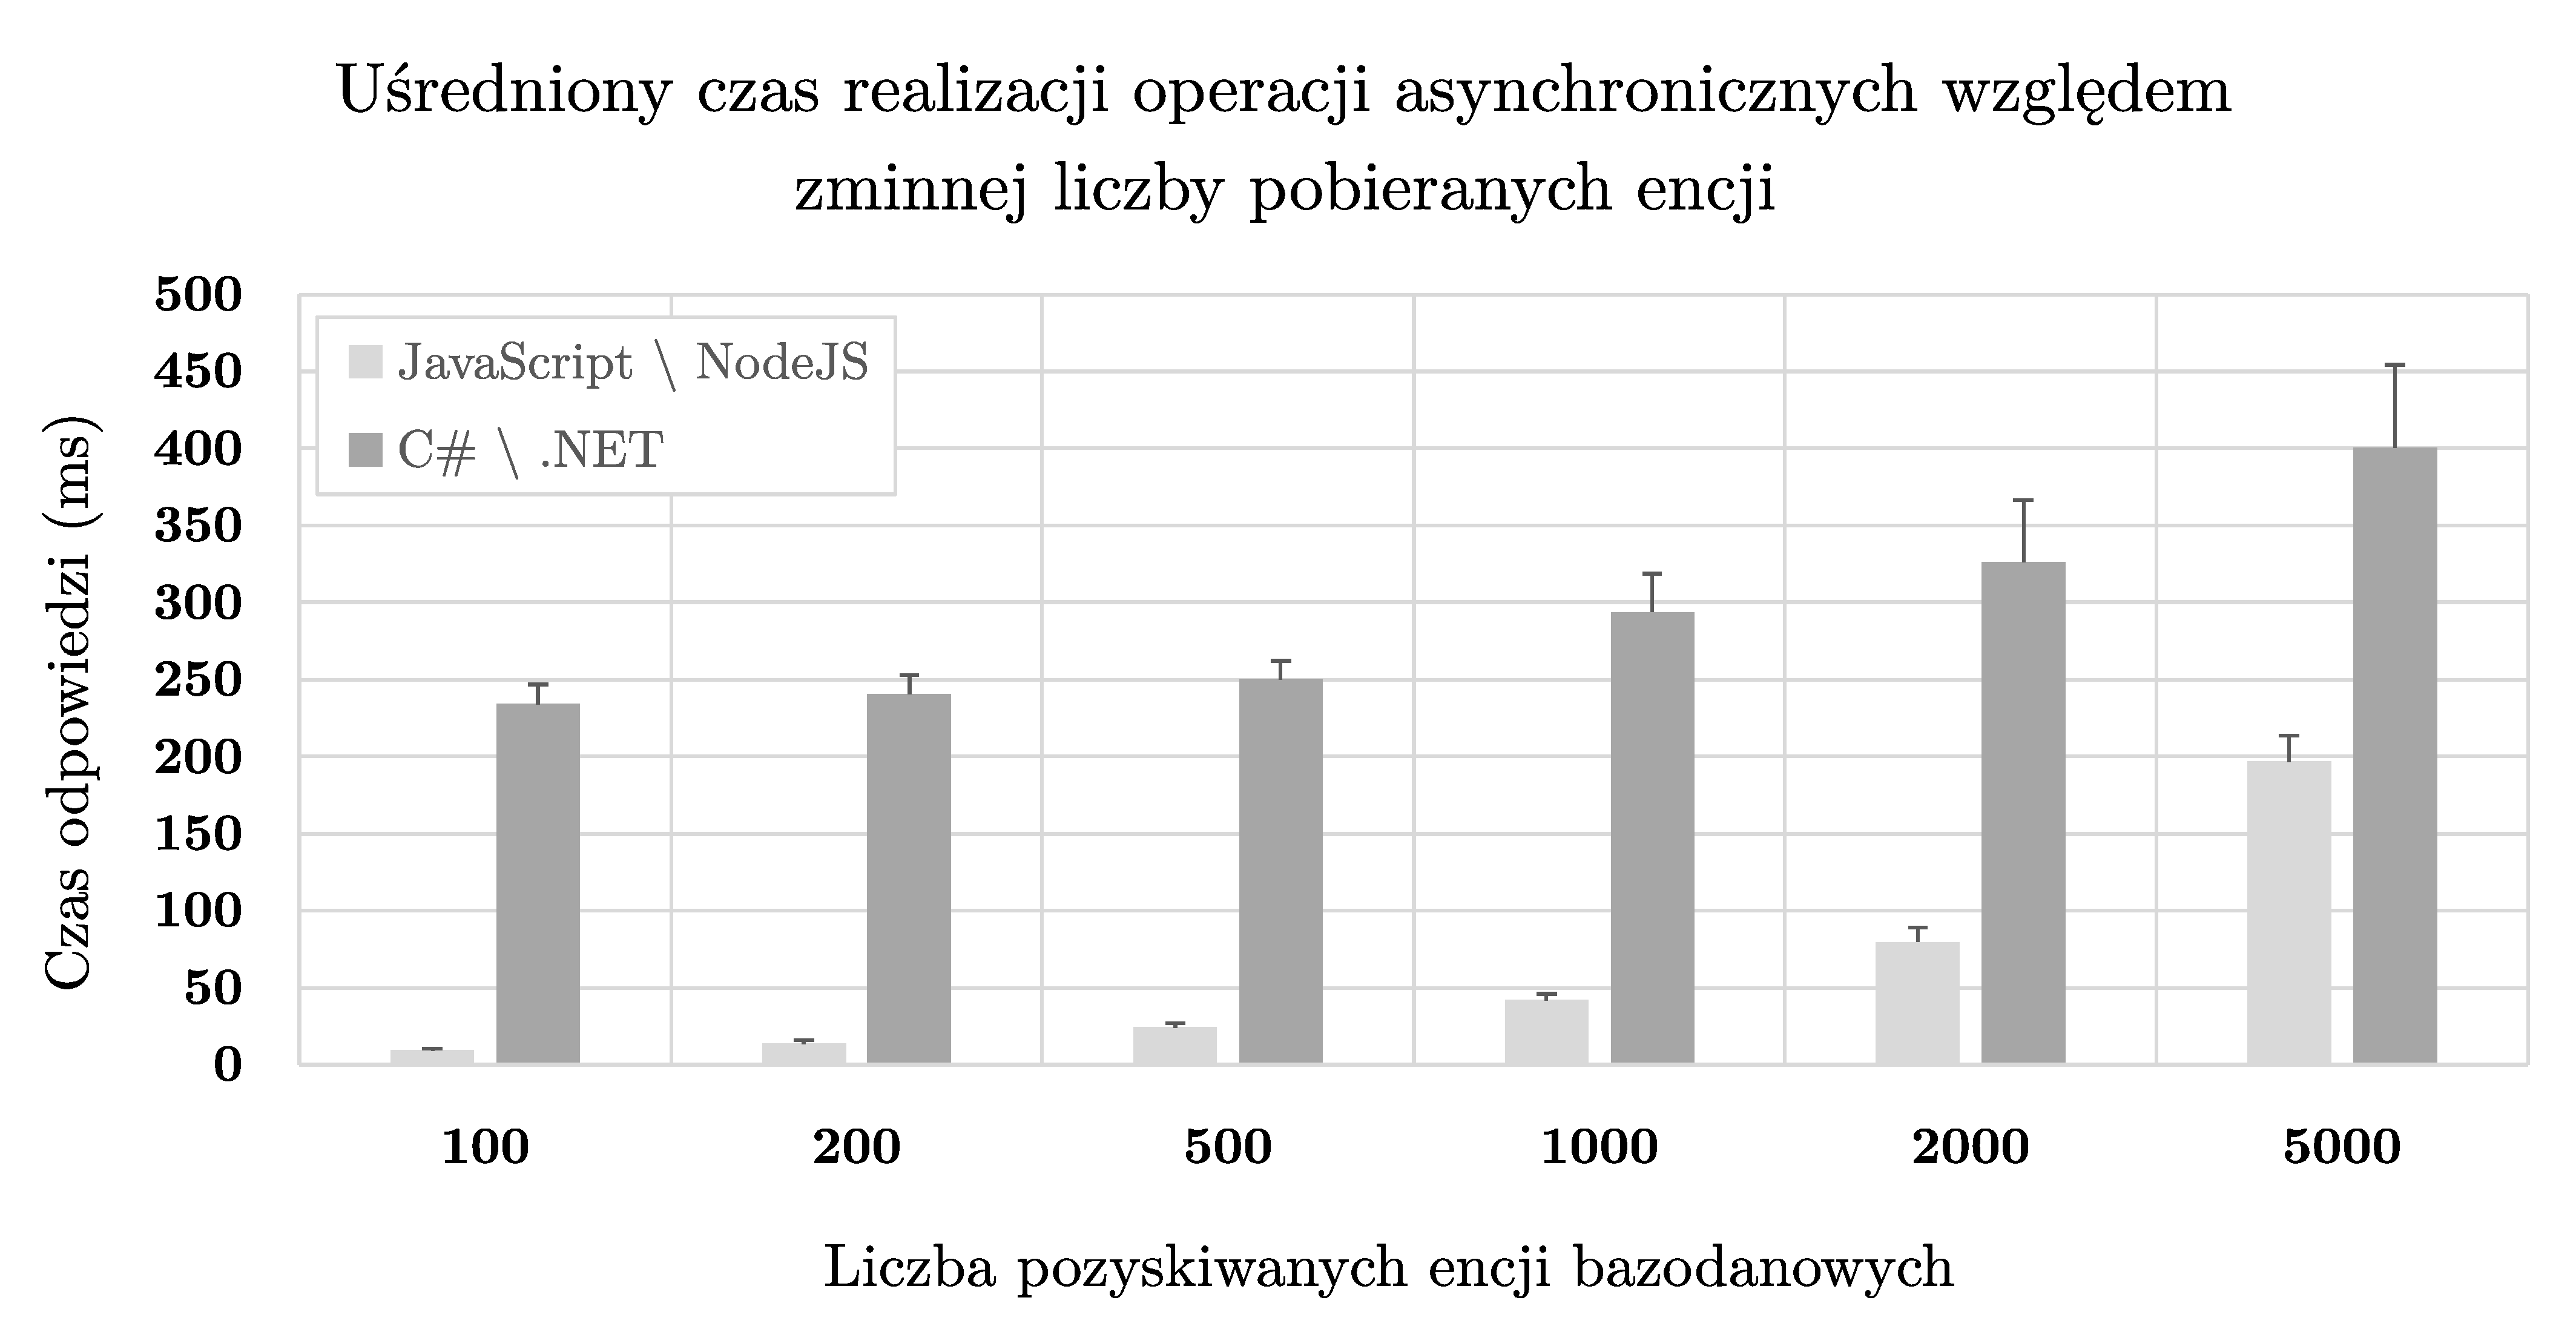
\includegraphics[width=\linewidth]{rys05/async-times.pdf}
  \caption{Uśredniony czas realizacji operacji asynchronicznych względem zmiennej liczby pobieranych encji}
  \label{fig:async-times}
\end{figure}

Zauważyć należy znaczącą wyższość rozwiązania opartego o technologie JavaScript / NodeJS, względem oprogramowania utworzonego z wykorzystaniem C\# .NET. Dla najmniejszej liczby pozyskiwanych encji, różnica średnich czasów odpowiedzi jest ponad 25 krotna. Wraz ze zwiększaniem liczebności pozyskiwanych obiektów modelu danych średni czas odpowiedzi dla NodeJS rośnie co prawda w szybszym tempie, niż ma to miejsce w kontekście rozwiązania uruchamianego na platformie .NET, jednakże nawet dla największej spośród liczb encji, dysproporcja wyników jest ponad dwukrotna. Warto zwrócić również uwagę na dyspersję poszczególnych rozwiązań względem przedstawionych średnich. Zaobserwować można zdecydowanie mniejsze odchylenia standardowe w odniesieniu do rozwiązania języka JavaScript, które zgodnie ze spodziewaną tendencją zwiększają się wraz z liczbą obiektów modelu danych. Dla dużych liczebności encji bazodanowych, rozwiązanie implementowane w języku C\# w niewielkiej liczbie przypadków uzyskuje wyniki bliskie średniej.

Tak znacząca dyferencja w kontekście obu interfejsów programowania aplikacji, wynikać może z implementacji natywnych rozwiązań klienta protokołu hipertekstowego. W środowisku NodeJS, klient ten posiada niewiele opcji konfiguracyjnych, a jakiekolwiek bardziej zaawansowane żądania, realizowane są z wykorzystaniem zewnętrznych bibliotek. Ponadto, klient ten, jest częścią rdzennego modułu środowiska NodeJS, obsługującego zoptymalizowaną komunikację hipertekstową. Rozwiązanie służące do komunikacji HTTP dla języka C\# jest mechanizmem dostarczanym przez biblioteki standardowe języka programowania, a nie samego środowiska uruchomieniowego. Oznacza to, że rozwiązanie dla tej właśnie technologii musi posiadać bardziej generyczną charakterystykę, aby móc być zastosowanym w dowolnym z przypadków użycia języka.
\section{Wpływ implementacji wzorca projektowego CQRS na wydajność obsługi żądania}
\label{sec:cqrs-and-database-improvements}
Celem niniejszego badania była obserwacja wpływu wdrożenia wzorca projektowego podziału odpowiedzialności, a także usprawnień wydajnościowych względem odseparowanych modeli encji, na wydajność obsługi żądań dla ocenianych interfejsów programowania aplikacji. Wdrożenie wzorca projektowego miało na celu odseparowanie operacji dotyczących odczytu danych, od tych, dokonujących ich modyfikacji. Separacja ta, występowała zarówno na poziomie logicznym (tj. modelu danych), jak i fizycznym (tj. systemu bazodanowego). Dzięki temu, możliwe było wprowadzenie optymalizacji wydajnościowych względem modelu odczytu. Aby zachować spójność informacji pomiędzy bazami danych, wprowadzono ponadto mechanizm replikacji transakcyjnej, działający w warstwie systemu bazodanowego. Po wysłaniu wiadomości modyfikującej dane, określony rekord jest zmieniany w bazie zapisu, a następnie wysyłany jest komunikat synchronizacji zmian w kierunku bazy odczytu. Szczegóły implementacyjne dotyczące omawianego badania przedstawiono w sekcji \ref{sec:implementacja-cqrs-i-replikacji}.

Zastosowany protokół badawczy posiada analogiczną strukturę do tego, który został zaprezentowany w badaniu wpływu systemów bazodanowych. Oznacza to, że w przedziale dwudziestu minut, stopniowo zwiększano liczbę współbieżnie pracujących wątków oprogramowania testowego, osiągając szczytową wartość równą 5000. W tym przypadku jednak, poddano analizie tylko pojedynczy system bazodanowy, który wspiera obsługę mechanizmu replikacji transakcyjnej - tj. Microsoft SQL Server. Kluczowym aspektem badania jest próba obserwacji czy, a także w jaki sposób wprowadzony model architektoniczny oraz usprawnienia wydajnościowe wpłyną na zmniejszenie się średniego czasu odpowiedzi, a także procentu błędnych odpowiedzi w stosunku do generowanych wiadomości. W badaniu zastosowano topologię fizyczną nr 4 przedstawioną w sekcji \ref{sec:lokalne-srodowisko-badawcze-ver-4}, a także plan testowy nr 1 wyszczególniony w punkcie \ref{plan-testowy-1}. Ogół przeprowadzonych operacji jest zgodny z wyspecyfikowanym scenariuszem badawczym nr 4 opisanym w tabeli \ref{tab:research-scenario-4}.

Na wykresach \ref{fig:3tier-vs-cqrs} a) do \ref{fig:3tier-vs-cqrs} d) przedstawiono kolejno porównanie procedur odczytu oraz zapisu, zarówno przed jak i po zastosowaniu omówionych modyfikacji.

\begin{figure}[htb]
  \centering
    \begin{tabular}{@{}ll@{}}
    a) & b) \\
    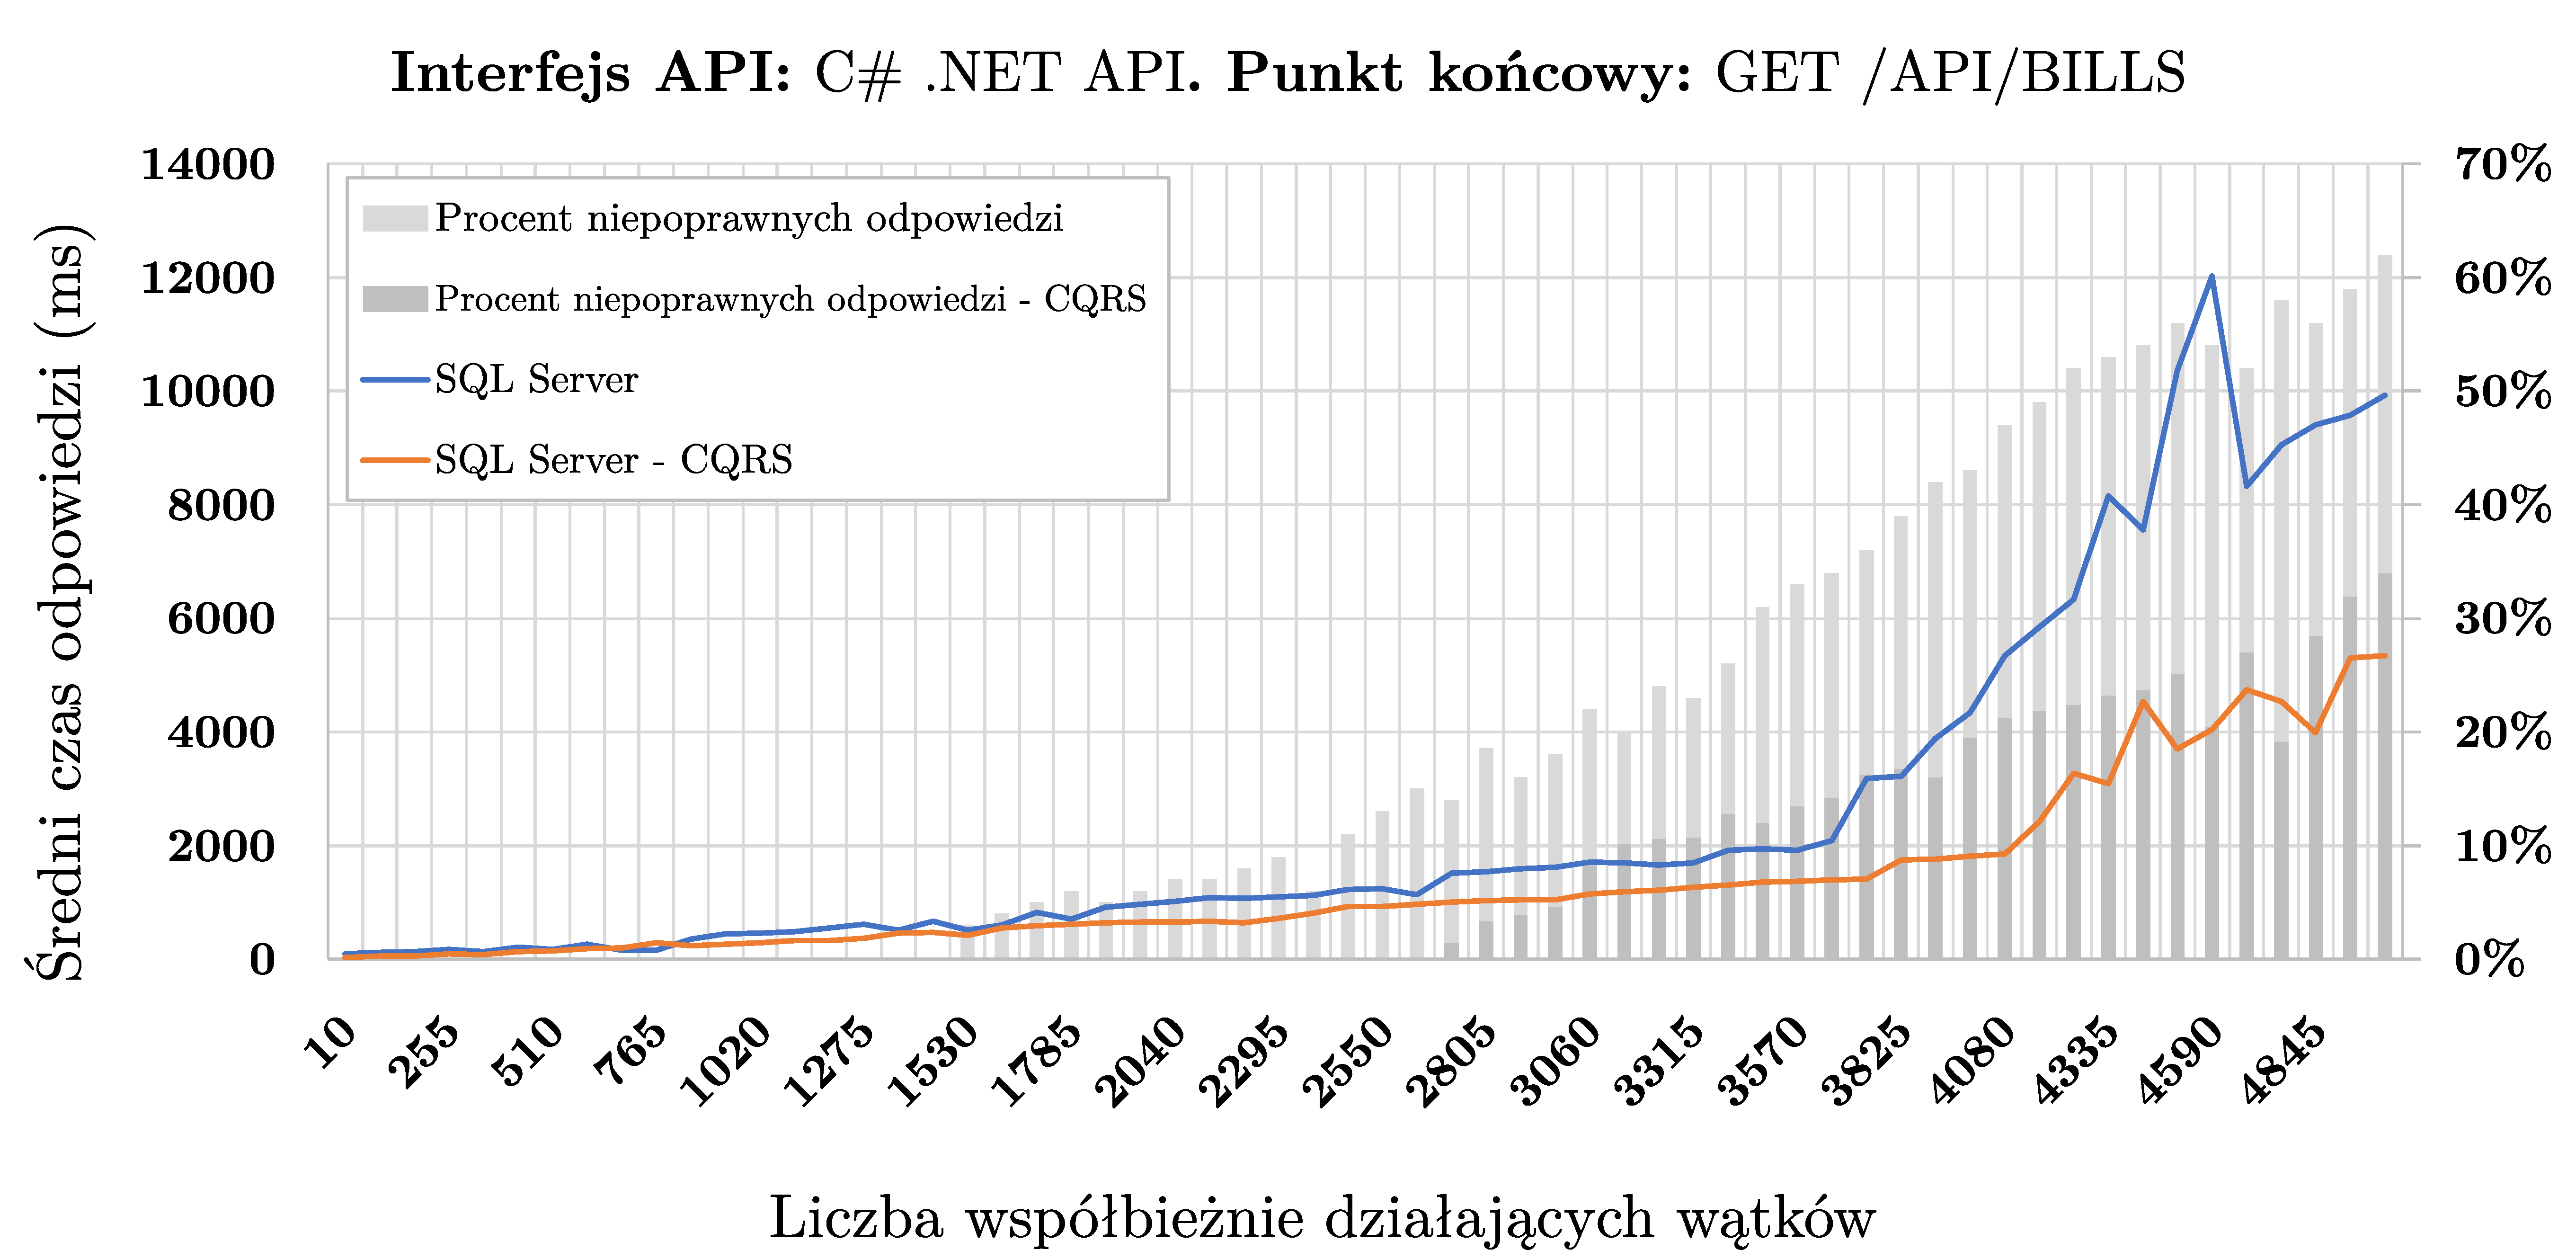
\includegraphics[width=0.49\textwidth]{rys05/dotnet-vs-cqrs.pdf} & 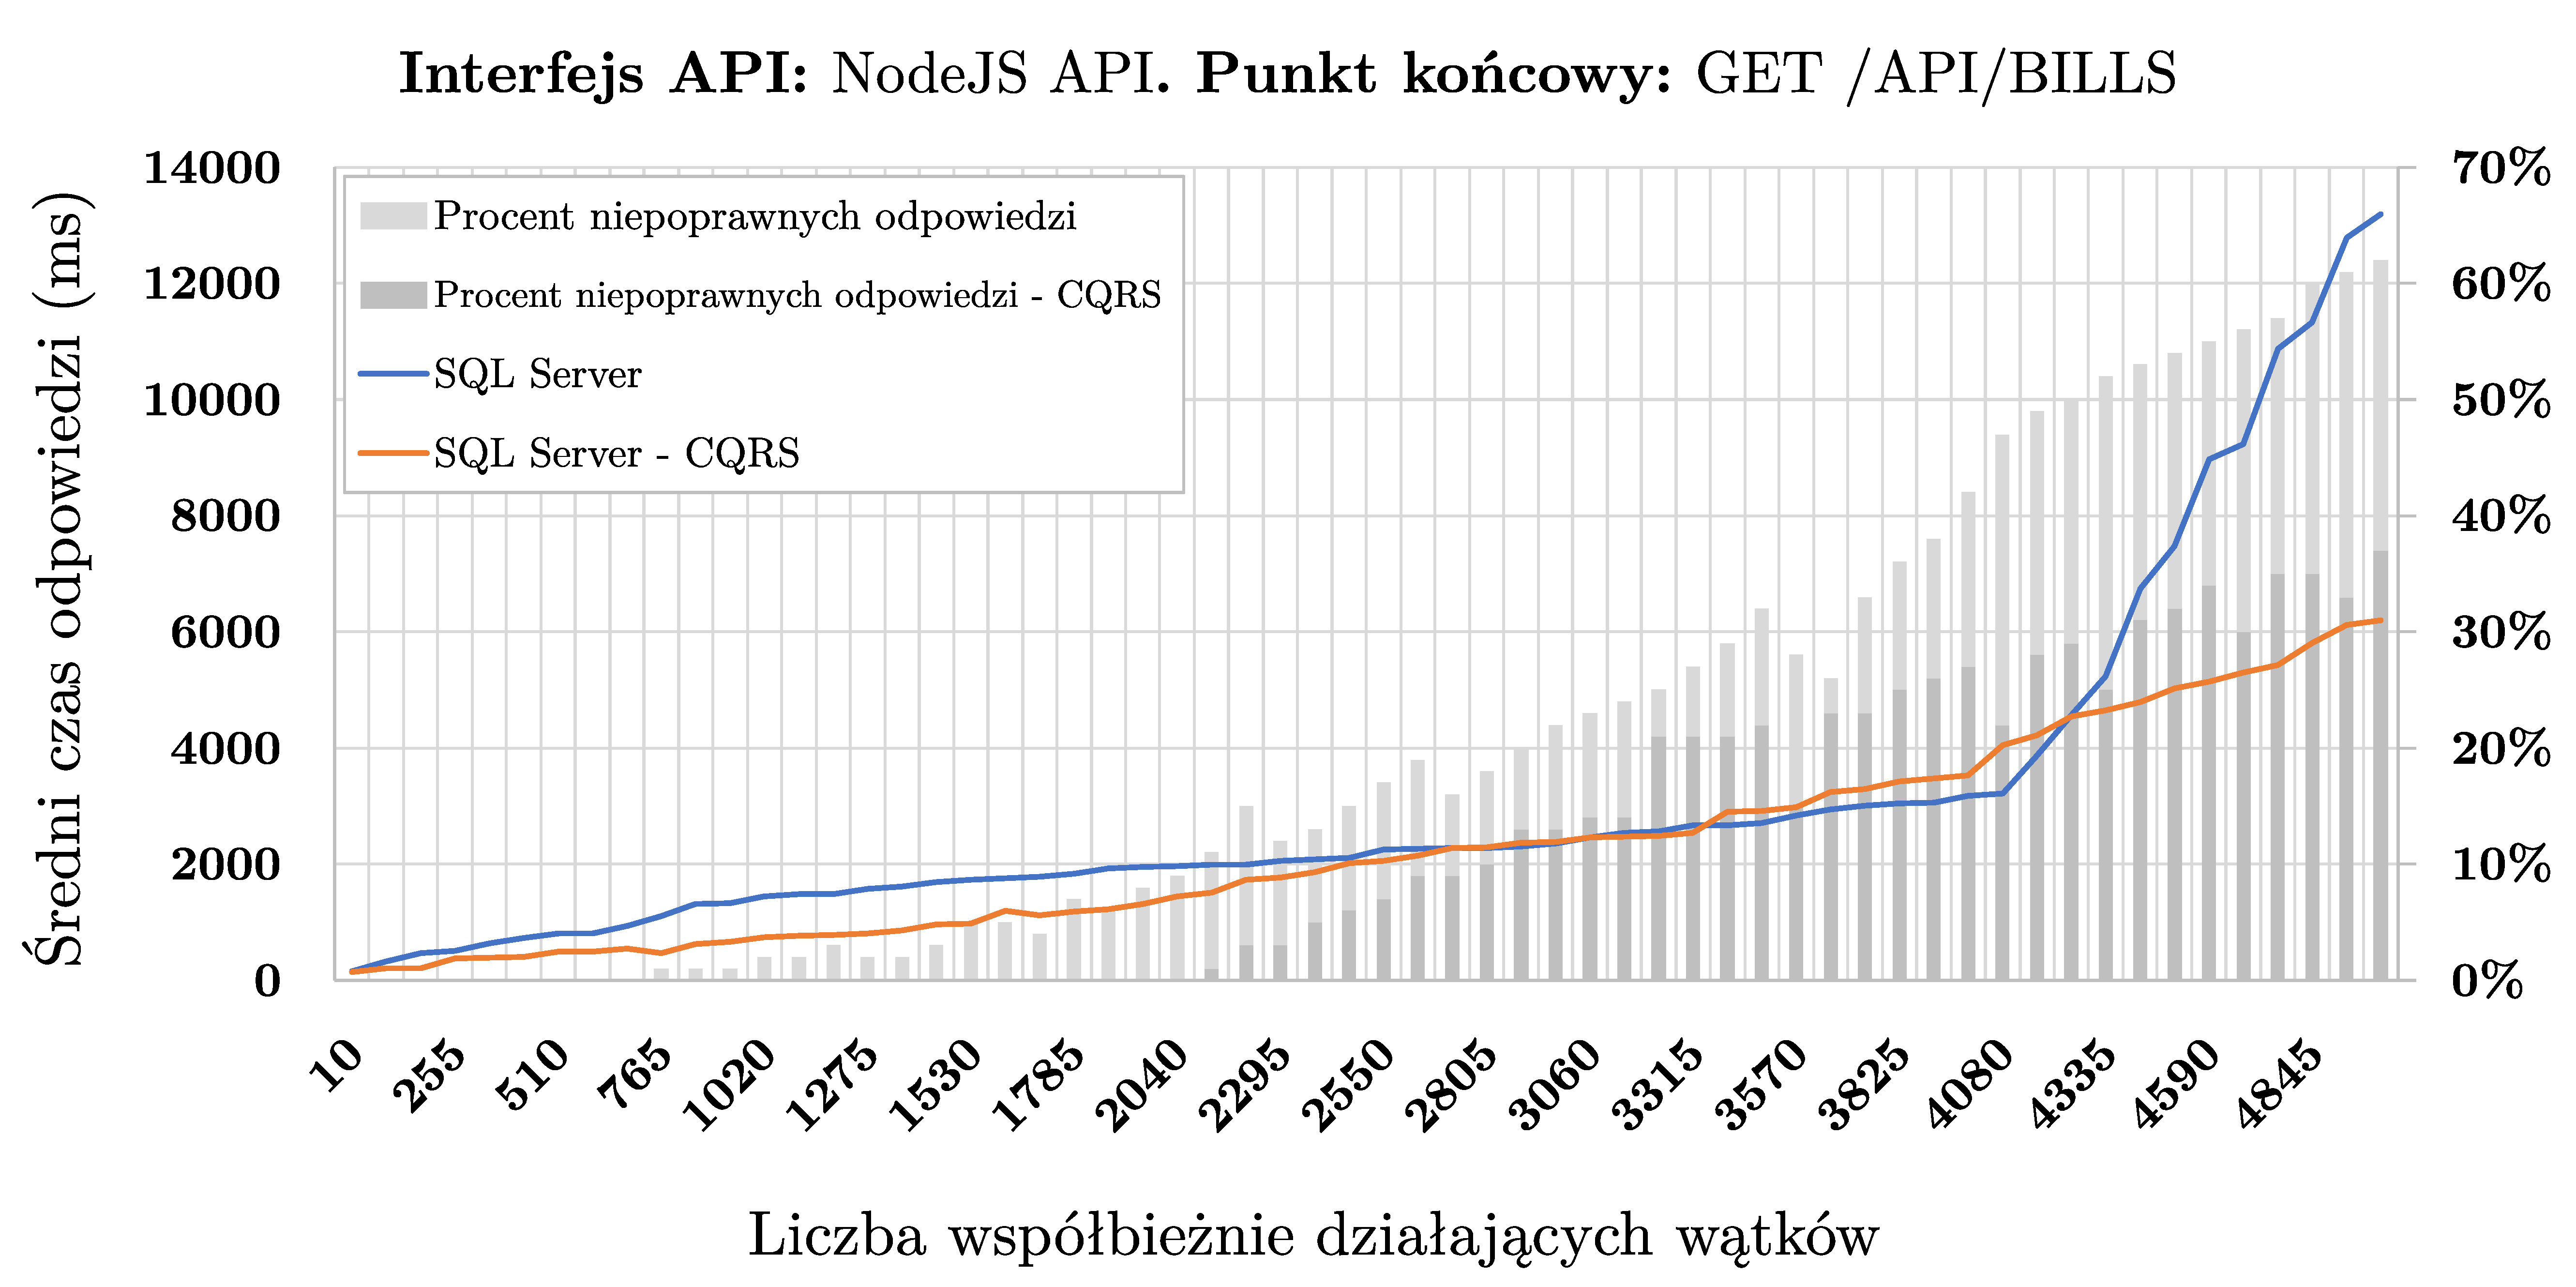
\includegraphics[width=0.49\textwidth]{rys05/nodejs-vs-cqrs.pdf} \\
    c) & d) \\
    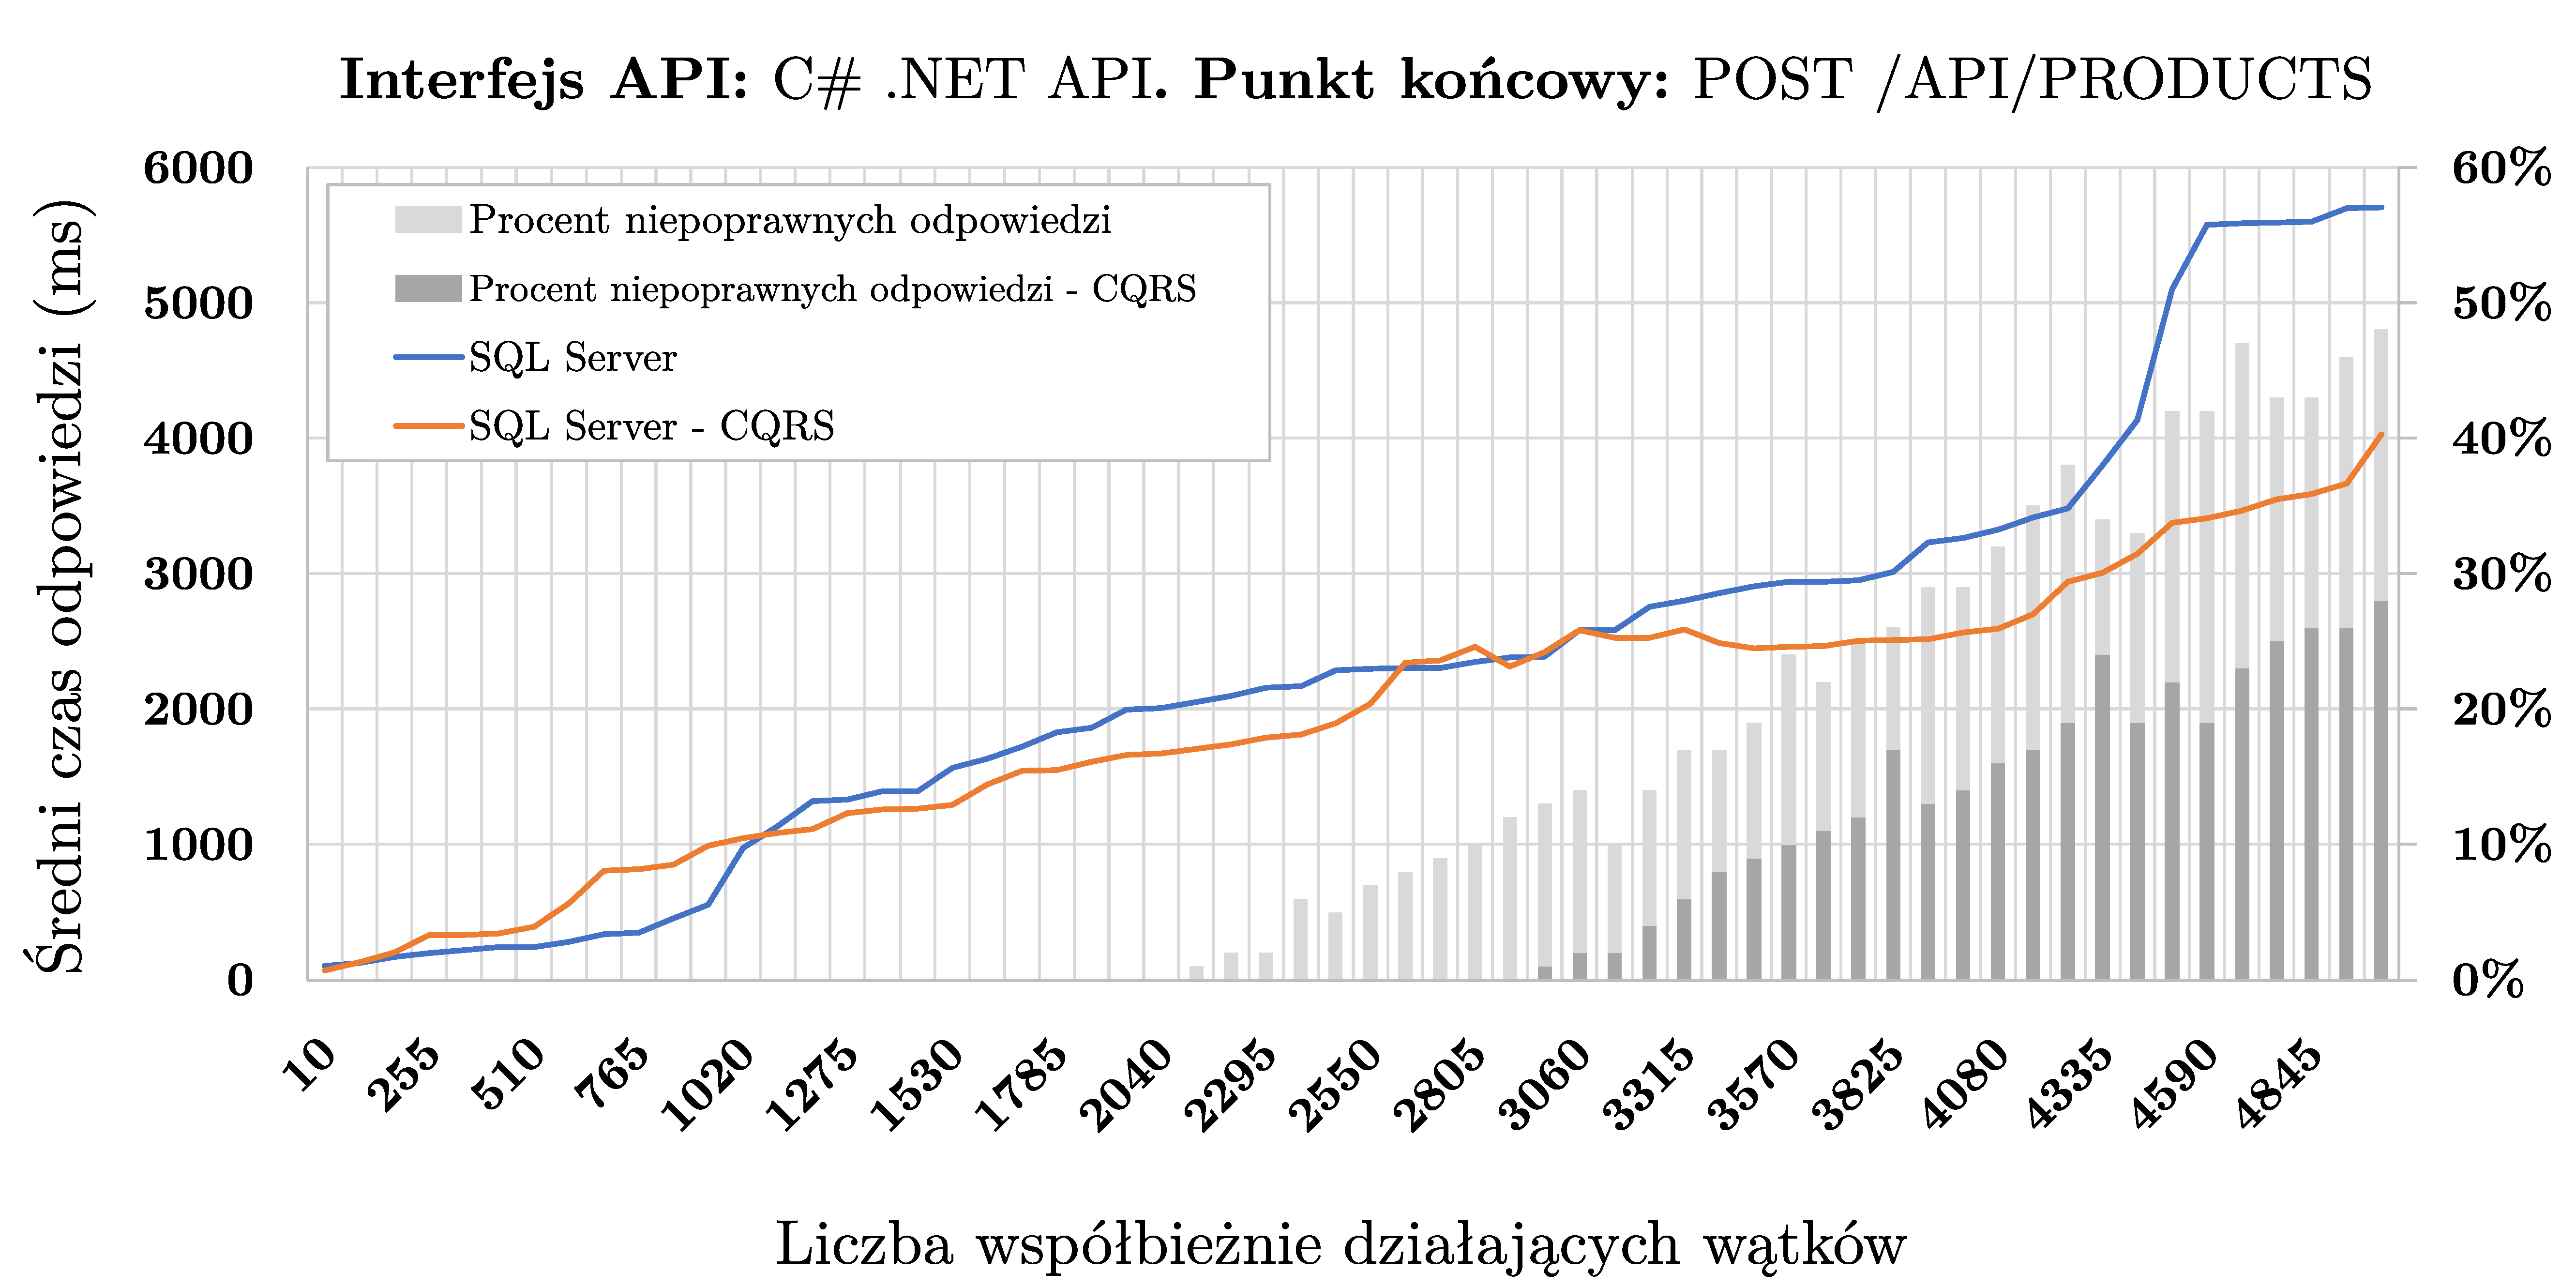
\includegraphics[width=0.49\textwidth]{rys05/dotnet-vs-cqrs-write.pdf} & 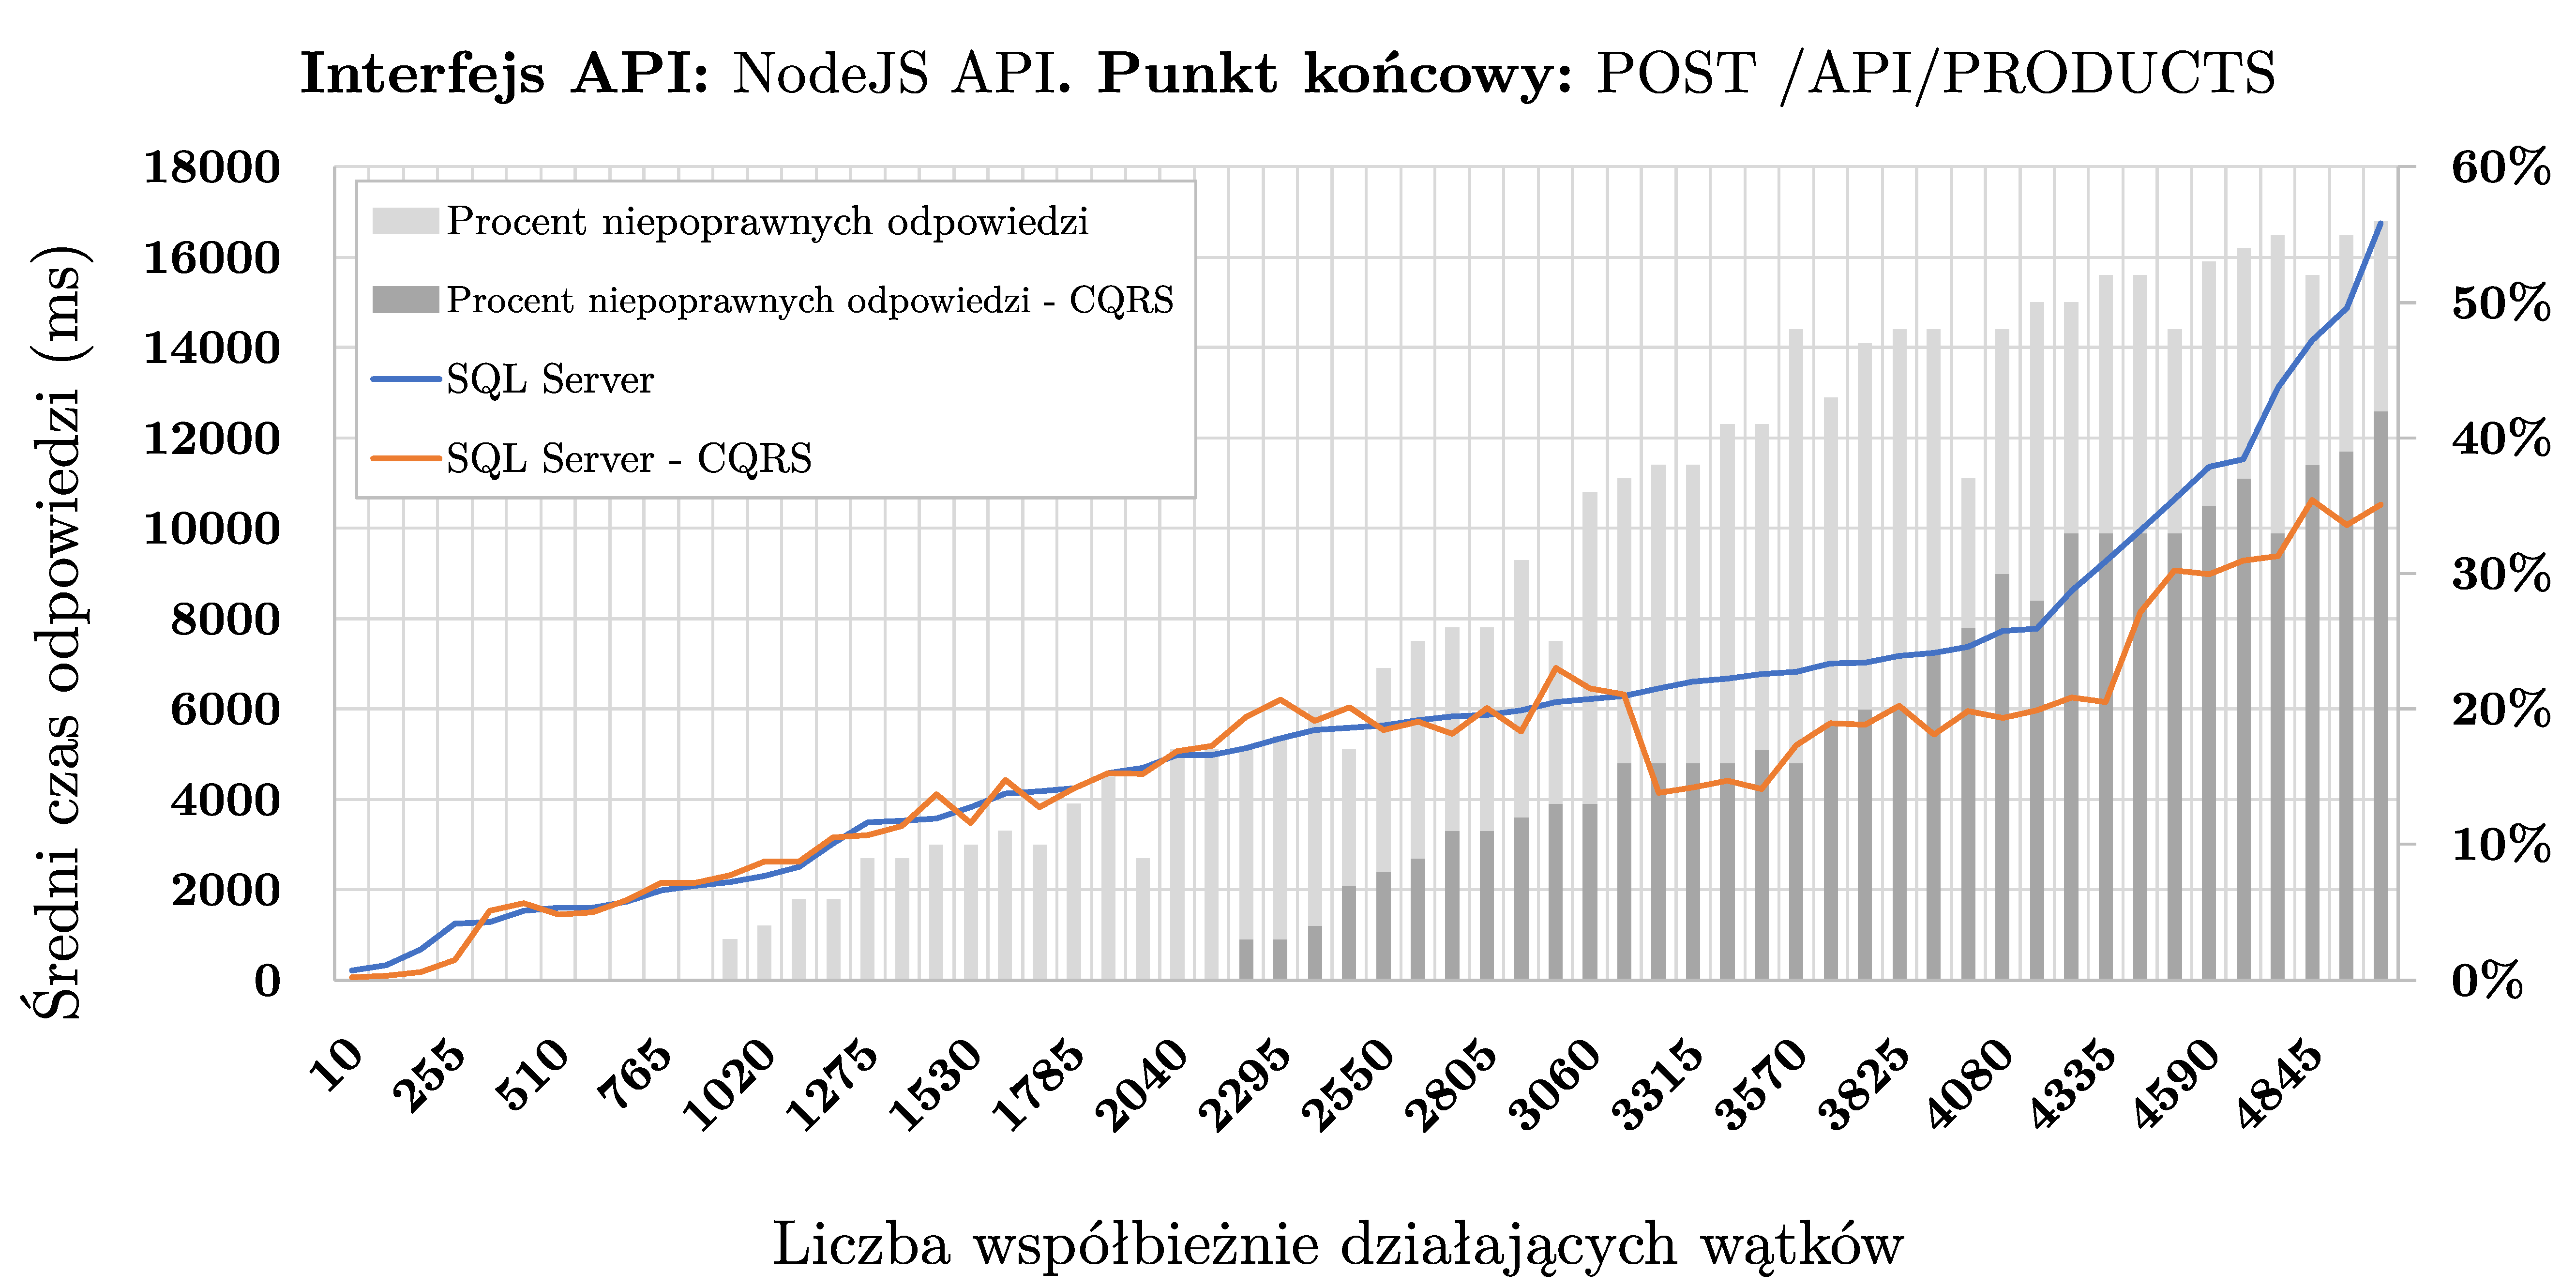
\includegraphics[width=0.49\textwidth]{rys05/nodejs-vs-cqrs-write.pdf}
    % jezeli obraki sa rownej wysokosci, mozna je wyrownac do gory stosujac vtop jak nizej
    % \vtop{\vskip-2ex\hbox{{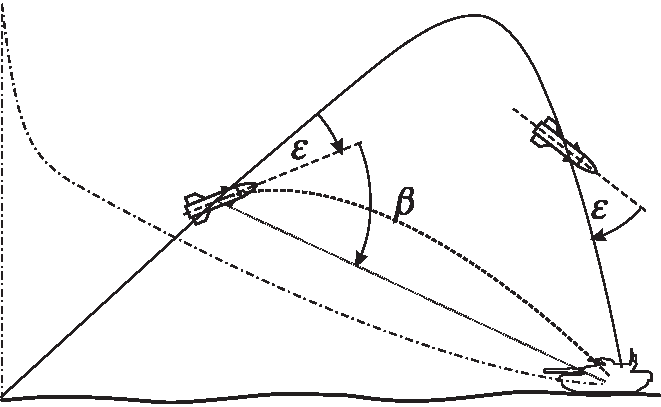
\includegraphics[width=0.475\textwidth]{rys05/beta1}}}} &
    % \vtop{\vskip-2ex\hbox{{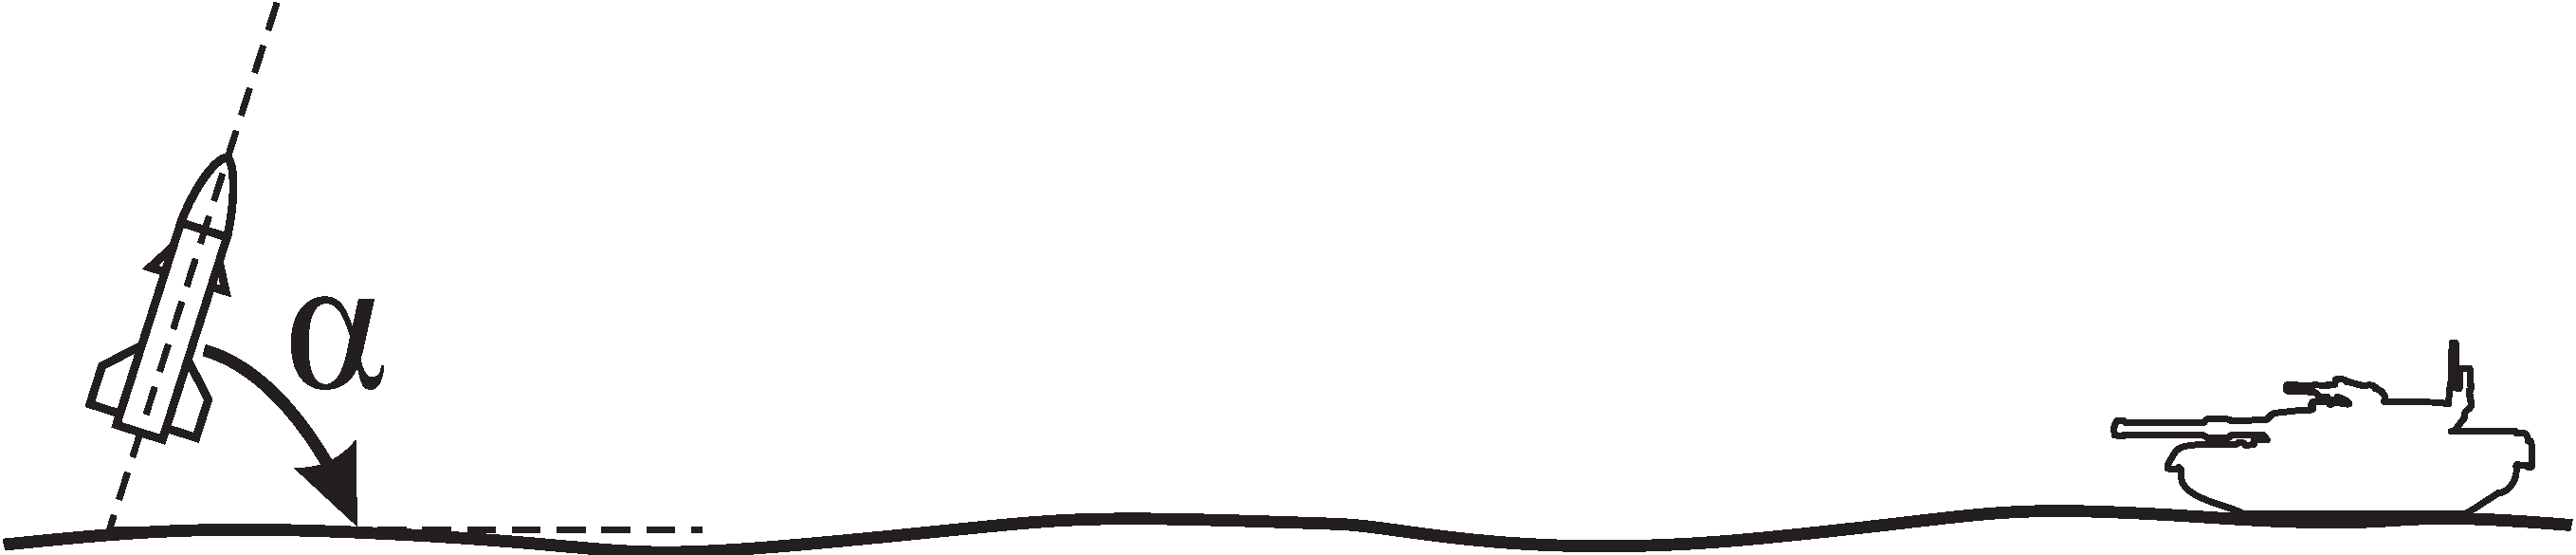
\includegraphics[width=0.475\textwidth]{rys05/alfa1}}}}  \caption{Wyznaczanie trajektorii lotu rakiety: 
    \end{tabular}
  \caption{Wydajność działania interfejsów API dla operacji odczytu oraz zapisu, przed i po zastosowaniu wzorca podziału odpowiedzialności}
  \label{fig:3tier-vs-cqrs}
\end{figure}

Dla każdego z przypadków zauważyć należy zarówno obniżenie się poziomu średniego czasu odpowiedzi, jak i procentowego błędu żądań niepoprawnych. Zachowanie takie, jest zrozumiałe ze względu na silną korelację obu metryk. Dostrzec należy relatywnie większą zmianę średniego czasu odpowiedzi w kontekście odczytu danych, niż ma to miejsce dla procedury ich zapisu. Wynika to z faktu, że dla zadania odczytu, dokonano usprawnień nie tylko związanych z komunikacją z bazą danych (m.in. zdefiniowanie puli połączeń), ale również dotyczących formułowania zapytań, czy też wewnętrznej struktury poszczególnych pól danych. Wpływ pierwszego z wymienionych w poprzednim zdaniu aspektów widoczny jest szczególnie w odniesieniu do zmiany procenta niepoprawnych żądań. Tyczy się to zarówno procedury odczytu, jak i zapisu. Co więcej metryka ta, wpływa na średni czas odpowiedzi. Czym więcej kanałów komunikacji z serwerem bazodanowym posiada interfejs API, tym więcej żądań będzie mógł on obsłużyć bez konieczności czekania na zwolnienie połączenia.

Dla procedury odczytu danych, po wprowadzeniu opisywanych w niniejszym badaniu usprawnień, pierwszy błąd związany z niepoprawną obsługą zapytania, pojawił się przy natężeniu o \textbf{1273} wątki wyższym dla api napisanego w technologii C\# .NET, oraz o \textbf{1527} wątków wyższym w przypadku NodeJS API. W kontekście metryki czasu wykonywania zapytania klienta, w momencie szczytowym zauważyć można różnicę \textbf{4577 ms} dla rozwiązania C\# oraz \textbf{6987 ms} dla systemu opartego o NodeJS.

Odnosząc się do procedury zapisu danych, przedział liczby wątków oprogramowania testowego, w ramach którego nie wystąpiły błędne żądania, rozszerzył się o \textbf{1190} procesów w przypadku interfejsu napisanego w języku JavaScript, a także o \textbf{765} procesów w przypadku api implementowanego w C\#. Doprowadziło to do spadku średniego czasu odpowiedzi w momencie szczytowym o \textbf{6225 ms} dla pierwszej z wymienionych technologii, a także o \textbf{1677 ms} dla drugiej z nich.

Analizując powyższe rezultaty, należy także spojrzeć na nie przez pryzmat ilości zmian, jakie zostały wprowadzone dla poszczególnych technologii. Mówiąc o interfejsie programowania aplikacji języka JavaScript, modyfikacje sprowadzały się do usprawnień na poziomie bazy danych, a także w kontekście momentu uruchamiania instancji mapera obiektowo-relacyjnego. Pomimo stosunkowo niewielkiej liczby zaimplementowanych adaptacji, wydajność rozwiązania wzrosła w sposób znaczący. Lekko odmienną tendencję zauważyć można dla usługi sieciowej napisanej w języku C\#. W tym przypadku wprowadzono nie tylko analogiczne względem konkurenta poprawki, ale także dodatkowo skorzystano z mechanizmów poprawy wydajności, specyficznych względem tylko tej technologii. Co prawda implementacja określonych modyfikacji wpłynęła pozytywnie na efektywność działania interfejsu, to zmiana ta, nie jest tak znacząca, jak dla rozwiązania opartego o technologię JavaScript / NodeJS. 
\section{Porównanie efektywności obsługi zapytań dla odmiennych mechanizmów pamięci podręcznej}
W przedstawionym badaniu dokonano porównania wydajności obsługi żądań klienckich, dotyczących pozyskiwania obiektów danych, w odniesieniu do wykorzystania zaimplementowanych mechanizmów pamięci podręcznej. Wydajność w ramach przeprowadzonej ewaluacji rozumiana była poprzez czas odpowiedzi na żądanie. Warto zaznaczyć, że nie uwzględniono parametru dotyczącego liczby niepoprawnych zapytań ponieważ dla żadnej z próbek, nie uzyskano nieprawidłowej odpowiedzi.

Zdecydowano się na wdrożenie dwóch mechanizmów obsługi pamięci podręcznej. Działanie pierwszego z nich, nazywanego mechanizmem statycznym, polega na zapamiętywaniu odpowiedzi w kontekście żądania o określonych właściwościach (tj. identyfikator zasobu, parametry zapytania), a także przetrzymywaniu jej w buforze przez stały, określony czas. Jeżeli zapytanie charakteryzujące się znaną uprzednio strukturą, zostanie odebrane w tym właśnie czasie, odpowiedź nie zostanie pobrana z bazy danych, a dostarczona bezpośrednio z omawianego bufora. Drugi mechanizm jest autorskim pomysłem twórcy niniejszej pracy i uwzględnia zmienność czasu przechowywania wpisu w odniesieniu do częstości wywoływań, a także unieważnień danych przechowywanych w pamięci cache. Mechanizm ten, wykorzystuje ponadto osobną strukturę danych, która jest aktualizowana przy wywołaniu dowolnego punktu końcowego, a gromadzone w niej dane, dostarczają informacji niezbędnych do wyliczania czasu zapamiętywania wpisu w cache. Niezależnie od omawianego mechanizmu, punkty końcowe odpowiedzialne za modyfikację danych, dla których wpisy przechowywane są w pamięci podręcznej, uruchamiają procedurę unieważnienia określonych obiektów encji. Szczegóły implementacyjne dotyczące obu mechanizmów pamięci podręcznej przytoczone zostały w sekcji \ref{sec:mechanizmy-cache}.

Odnosząc się do procedury badawczej, wykonane zostało 20 eksperymentów, w ramach których 30 współbieżnie pracujących wątków generowało żądania w kierunku dwóch punktów końcowych. Pierwszy z nich, dotyczył pobrania listy encji o stałym rozmiarze, natomiast drugi -- uzyskania pojedynczego obiektu danych. Dla każdej z ewaluacji, przeprowadzanej w kontekście określonego interfejsu programowania aplikacji, zdefiniowano pięć zdarzeń unieważnienia danych (tj. momentów wywołania punktu końcowego modyfikującego encje). Ponadto zaznaczyć należy, że czas trwania pojedynczego eksperymentu był stały i wynosił 20 minut. Co więcej, wprowadzona została celowa dysproporcja pomiędzy liczbą żądań pozyskujących listę obiektów, a liczbą zapytań, których rezultatem jest zwrócenie tylko jednego z nich. Stosunek ten, wynosił dwa do jednego. Taka struktura badań, wynika z charakterystyki dotyczącej sposobu wyliczania czasu przechowywania wpisu w pamięci podręcznej w odniesieniu do autorskiego mechanizmu. Promuje on, te spośród żądań, których częstotliwość wywołań jest większa.

Dla statycznego mechanizmu pamięci cache zastosowano czas życia wynoszący 60s, podczas gdy czasem referencyjnym mechanizmu autorskiego było 120s. Co więcej, wewnętrzna struktura wykorzystywana w rozwiązaniu autorskim, została wygenerowana na podstawie liczby żądań wysłanych w czasie realizacji eksperymentu ze stałym czasem przechowywania wpisu. Dzięki temu, punkt końcowy dotyczący pobierania listy elementów, był postrzegany jako element wywoływany z większą częstotliwością.

Badanie przeprowadzono zgodnie z koncepcją zarysowaną w scenariuszu badawczym nr 5, którego elementy wyspecyfikowano w tabeli \ref{tab:research-scenario-5}, a także wykorzystując konfigurację nr 2 lokalnej topologii fizycznej przedstawionej w sekcji \ref{sec:lokalne-srodowisko-badawcze-ver-2}.

W tabeli \ref{tab:mtc-5-table} zaprezentowano elementy charakterystyczne dla każdego z dwudziestu eksperymentów, a także rezultaty jakie w kontekście nich odnotowano.

\begin{table}[H] \small
\centering
\caption{Wydajność metod obsługi pamięci podręcznej względem technologii oraz momentu unieważnienia wpisu}
\label{tab:mtc-5-table}
\resizebox{\columnwidth}{!}{%
\begin{tabular}{|l|l|ccccc|l|l|}
\hline
\multirow{2}{*}{} &
  \multirow{2}{*}{Typ metody} &
  \multicolumn{5}{c|}{Moment unieważnienia} &
  \multirow{2}{*}{\begin{tabular}[c]{@{}l@{}}Liczba żądań\\ \textgreater 500 ms\end{tabular}} &
  \multirow{2}{*}{\begin{tabular}[c]{@{}l@{}}Zysk względem\\ rozwiązania alternatywnego\end{tabular}} \\ \cline{3-7}
  &
   &
  \multicolumn{1}{c|}{\#1} &
  \multicolumn{1}{c|}{\#2} &
  \multicolumn{1}{c|}{\#3} &
  \multicolumn{1}{c|}{\#4} &
  \#5 &
   &
   \\ \hline\hline\
\multirow{2}{*}{C\# / .NET} &
  statyczna &
  \multicolumn{1}{c|}{06:40} &
  \multicolumn{1}{c|}{10:00} &
  \multicolumn{1}{c|}{13:20} &
  \multicolumn{1}{c|}{15:00} &
  19:40 &
  10 &
  - \\ \cline{2-9} 
 &
  \textbf{autorska} &
  \multicolumn{1}{c|}{06:40} &
  \multicolumn{1}{c|}{10:00} &
  \multicolumn{1}{c|}{13:20} &
  \multicolumn{1}{c|}{15:00} &
  19:40 &
  9 &
  13,77 ms \\ \hline
\multirow{2}{*}{C\# / .NET} &
  statyczna &
  \multicolumn{1}{c|}{00:32} &
  \multicolumn{1}{c|}{03:45} &
  \multicolumn{1}{c|}{06:52} &
  \multicolumn{1}{c|}{07:49} &
  16:40 &
  8 &
  20,16 ms \\ \cline{2-9} 
 &
  autorska &
  \multicolumn{1}{c|}{00:32} &
  \multicolumn{1}{c|}{03:45} &
  \multicolumn{1}{c|}{06:52} &
  \multicolumn{1}{c|}{07:49} &
  16:40 &
  12 &
  - \\ \hline
\multirow{2}{*}{C\# / .NET} &
  statyczna &
  \multicolumn{1}{c|}{02:44} &
  \multicolumn{1}{c|}{06:30} &
  \multicolumn{1}{c|}{14:27} &
  \multicolumn{1}{c|}{16:55} &
  19:42 &
  14 &
  - \\ \cline{2-9} 
 &
  \textbf{autorska} &
  \multicolumn{1}{c|}{02:44} &
  \multicolumn{1}{c|}{06:30} &
  \multicolumn{1}{c|}{14:27} &
  \multicolumn{1}{c|}{16:55} &
  19:42 &
  10 &
  12,54 ms \\ \hline
\multirow{2}{*}{C\# / .NET} &
  statyczna &
  \multicolumn{1}{c|}{01:15} &
  \multicolumn{1}{c|}{05:29} &
  \multicolumn{1}{c|}{08:31} &
  \multicolumn{1}{c|}{14:48} &
  17:45 &
  15 &
  - \\ \cline{2-9} 
 &
  \textbf{autorska} &
  \multicolumn{1}{c|}{01:15} &
  \multicolumn{1}{c|}{05:29} &
  \multicolumn{1}{c|}{08:31} &
  \multicolumn{1}{c|}{14:48} &
  17:45 &
  13 &
  19,29 ms \\ \hline
\multirow{2}{*}{C\# / .NET} &
  statyczna &
  \multicolumn{1}{c|}{02:01} &
  \multicolumn{1}{c|}{07:32} &
  \multicolumn{1}{c|}{12:00} &
  \multicolumn{1}{c|}{13:27} &
  15:56 &
  16 &
  24,85 ms \\ \cline{2-9} 
 &
  autorska &
  \multicolumn{1}{c|}{02:01} &
  \multicolumn{1}{c|}{07:32} &
  \multicolumn{1}{c|}{12:00} &
  \multicolumn{1}{c|}{13:27} &
  15:56 &
  20 &
  - \\ \hline
\multirow{2}{*}{JS / NodeJS} &
  statyczna &
  \multicolumn{1}{c|}{06:40} &
  \multicolumn{1}{c|}{10:00} &
  \multicolumn{1}{c|}{13:20} &
  \multicolumn{1}{c|}{15:00} &
  19:40 &
  17 &
  - \\ \cline{2-9} 
 &
  \textbf{autorska} &
  \multicolumn{1}{c|}{06:40} &
  \multicolumn{1}{c|}{10:00} &
  \multicolumn{1}{c|}{13:20} &
  \multicolumn{1}{c|}{15:00} &
  19:40 &
  14 &
  18,13ms \\ \hline
\multirow{2}{*}{JS / NodeJS} &
  statyczna &
  \multicolumn{1}{c|}{00:32} &
  \multicolumn{1}{c|}{03:45} &
  \multicolumn{1}{c|}{06:52} &
  \multicolumn{1}{c|}{07:49} &
  16:40 &
  13 &
  23,14 ms \\ \cline{2-9} 
 &
  autorska &
  \multicolumn{1}{c|}{00:32} &
  \multicolumn{1}{c|}{03:45} &
  \multicolumn{1}{c|}{06:52} &
  \multicolumn{1}{c|}{07:49} &
  16:40 &
  15 &
  - \\ \hline
\multirow{2}{*}{JS / NodeJS} &
  statyczna &
  \multicolumn{1}{c|}{02:44} &
  \multicolumn{1}{c|}{06:30} &
  \multicolumn{1}{c|}{14:27} &
  \multicolumn{1}{c|}{16:55} &
  19:42 &
  11 &
  11,97 ms \\ \cline{2-9} 
 &
  autorska &
  \multicolumn{1}{c|}{02:44} &
  \multicolumn{1}{c|}{06:30} &
  \multicolumn{1}{c|}{14:27} &
  \multicolumn{1}{c|}{16:55} &
  19:42 &
  16 &
  - \\ \hline
\multirow{2}{*}{JS / NodeJS} &
  statyczna &
  \multicolumn{1}{c|}{01:15} &
  \multicolumn{1}{c|}{05:29} &
  \multicolumn{1}{c|}{08:31} &
  \multicolumn{1}{c|}{14:48} &
  17:45 &
  14 &
  - \\ \cline{2-9} 
 &
  \textbf{autorska} &
  \multicolumn{1}{c|}{01:15} &
  \multicolumn{1}{c|}{05:29} &
  \multicolumn{1}{c|}{08:31} &
  \multicolumn{1}{c|}{14:48} &
  17:45 &
  8 &
  21,91 ms \\ \hline
\multirow{2}{*}{JS / NodeJS} &
  statyczna &
  \multicolumn{1}{c|}{02:01} &
  \multicolumn{1}{c|}{07:32} &
  \multicolumn{1}{c|}{12:00} &
  \multicolumn{1}{c|}{13:27} &
  15:56 &
  15 &
  - \\ \cline{2-9} 
 &
  \textbf{autorska} &
  \multicolumn{1}{c|}{02:01} &
  \multicolumn{1}{c|}{07:32} &
  \multicolumn{1}{c|}{12:00} &
  \multicolumn{1}{c|}{13:27} &
  15:56 &
  13 &
  14,35 ms \\ \hline
\end{tabular}%
}
\end{table}

Moment unieważnienia rozumiany jest jako punkt na osi czasu, kiedy nastąpiło wywołanie żądania aktualizacji encji bazodanowych. Czasy odpowiedzi na żądanie oraz liczby żądań powyżej 500 ms odnoszą się do punktu końcowego pozyskiwania kolekcji obiektów danych.

Zauważyć należy, że autorskie rozwiązanie zakładające zmienny czas przechowywania wpisu w pamięci podręcznej, notuje zysk względem rozwiązania konkurencyjnego w sześciu przypadkach na dziesięć zdefiniowanych. Minimalna wartość zysku, w kontekście eksperymentów to \textbf{12,54 ms} -- interfejs programowania C\# .NET, natomiast maksymalna to \textbf{21,91 ms} -- interfejs JavaScript / NodeJS. Niewątpliwie, zaobserwować można silną korelację pomiędzy wartością omawianego zysku a liczbą żądań, których czas trwania wynosi ponad 500 ms. Bardzo prawdopodobnym jest, że dla większości z tych zapytań, realizowana jest komunikacja z bazą danych wskutek braku określonego wpisu w pamięci cache. Analizując przewagi rozwiązań w obrębie każdego z eksperymentów, zauważyć można, że za każdym razem, gdy liczba żądań o czasie odpowiedzi powyżej 500 ms jest wyższa, to przekłada się to na gorszy wynik średni.

Ponadto, wartym odnotowania jest fakt, że autorskie rozwiązanie zarządzania wpisami pamięci podręcznej, wykazuje lepsze rezultaty w tych przypadkach, kiedy zakresy pomiędzy momentami unieważnień są stosunkowo szerokie. W związku z uzyskaniem dłuższego czasu życia przez określony element gromadzony w pamięci podręcznej, żądanie pobierające dane z systemu bazodanowego może zostać opóźnione, a co za tym idzie, średni czas odpowiedzi może być niższy. Sytuacja staje się z goła odmienna, z chwilą częstej inwalidacji wpisu pamięci cache na przestrzeni czasu, co prowadzi do ograniczenia długości czasu jego życia.

Na wykresach \ref{fig:cache-charts} a) do \ref{fig:cache-charts} d) pokazano faktyczne czasy odpowiedzi, dla żądań generowanych w kontekście pierwszego z eksperymentów przedstawionych w tabeli.

\begin{figure}[htb]
  \centering
    \begin{tabular}{@{}ll@{}}
    a) & b) \\
    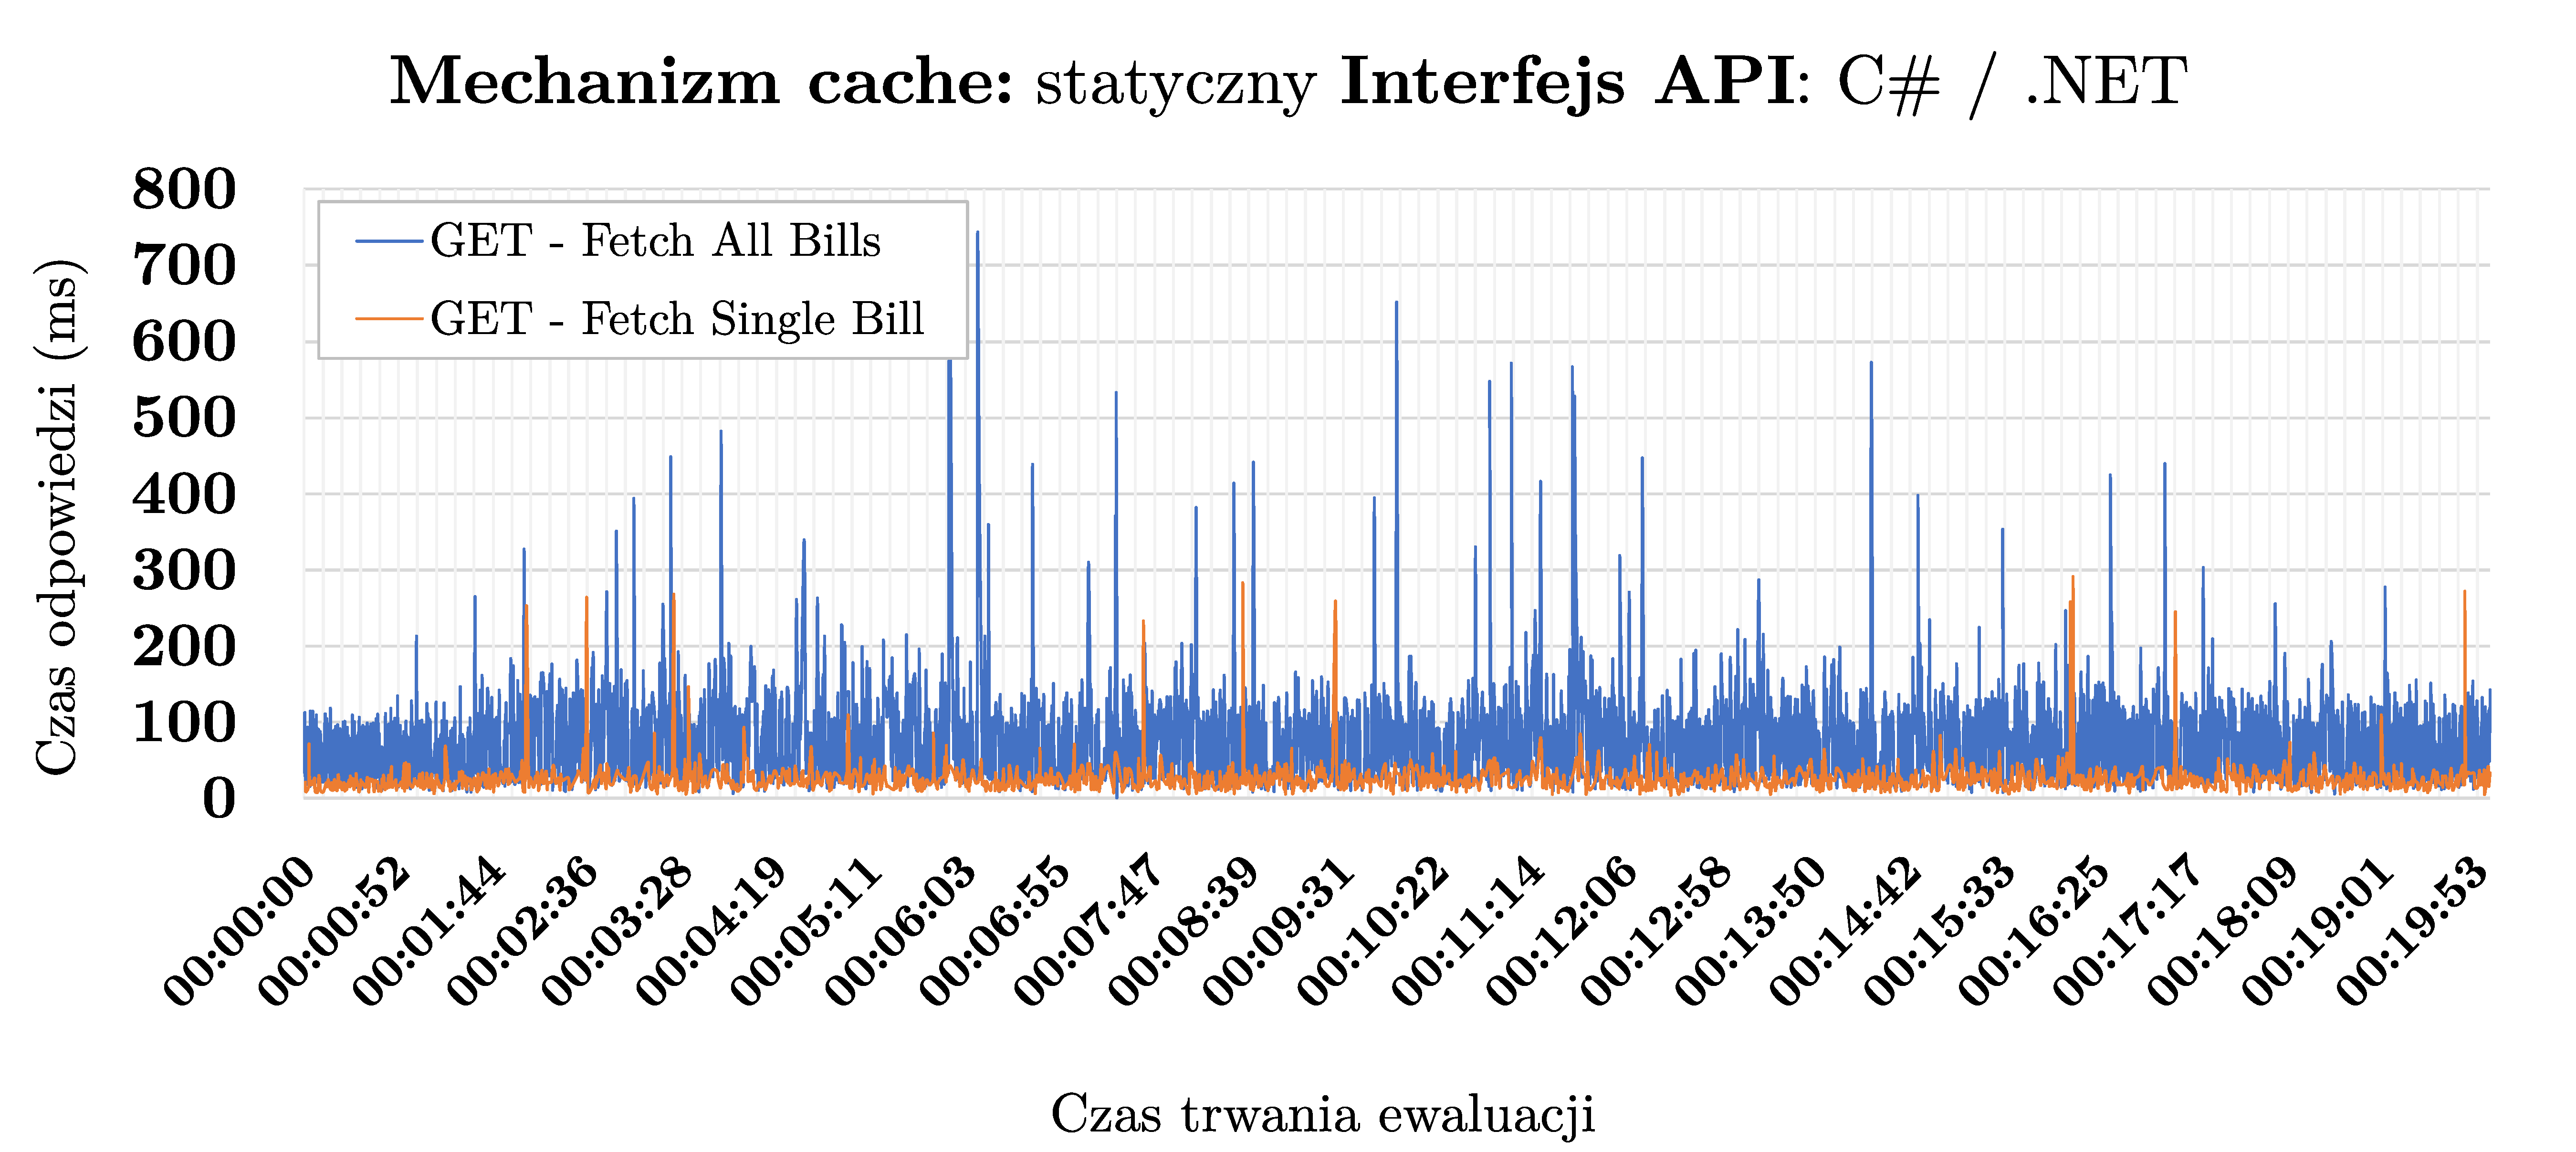
\includegraphics[width=0.49\textwidth]{rys05/dotnet-static-cache-chart.pdf} & 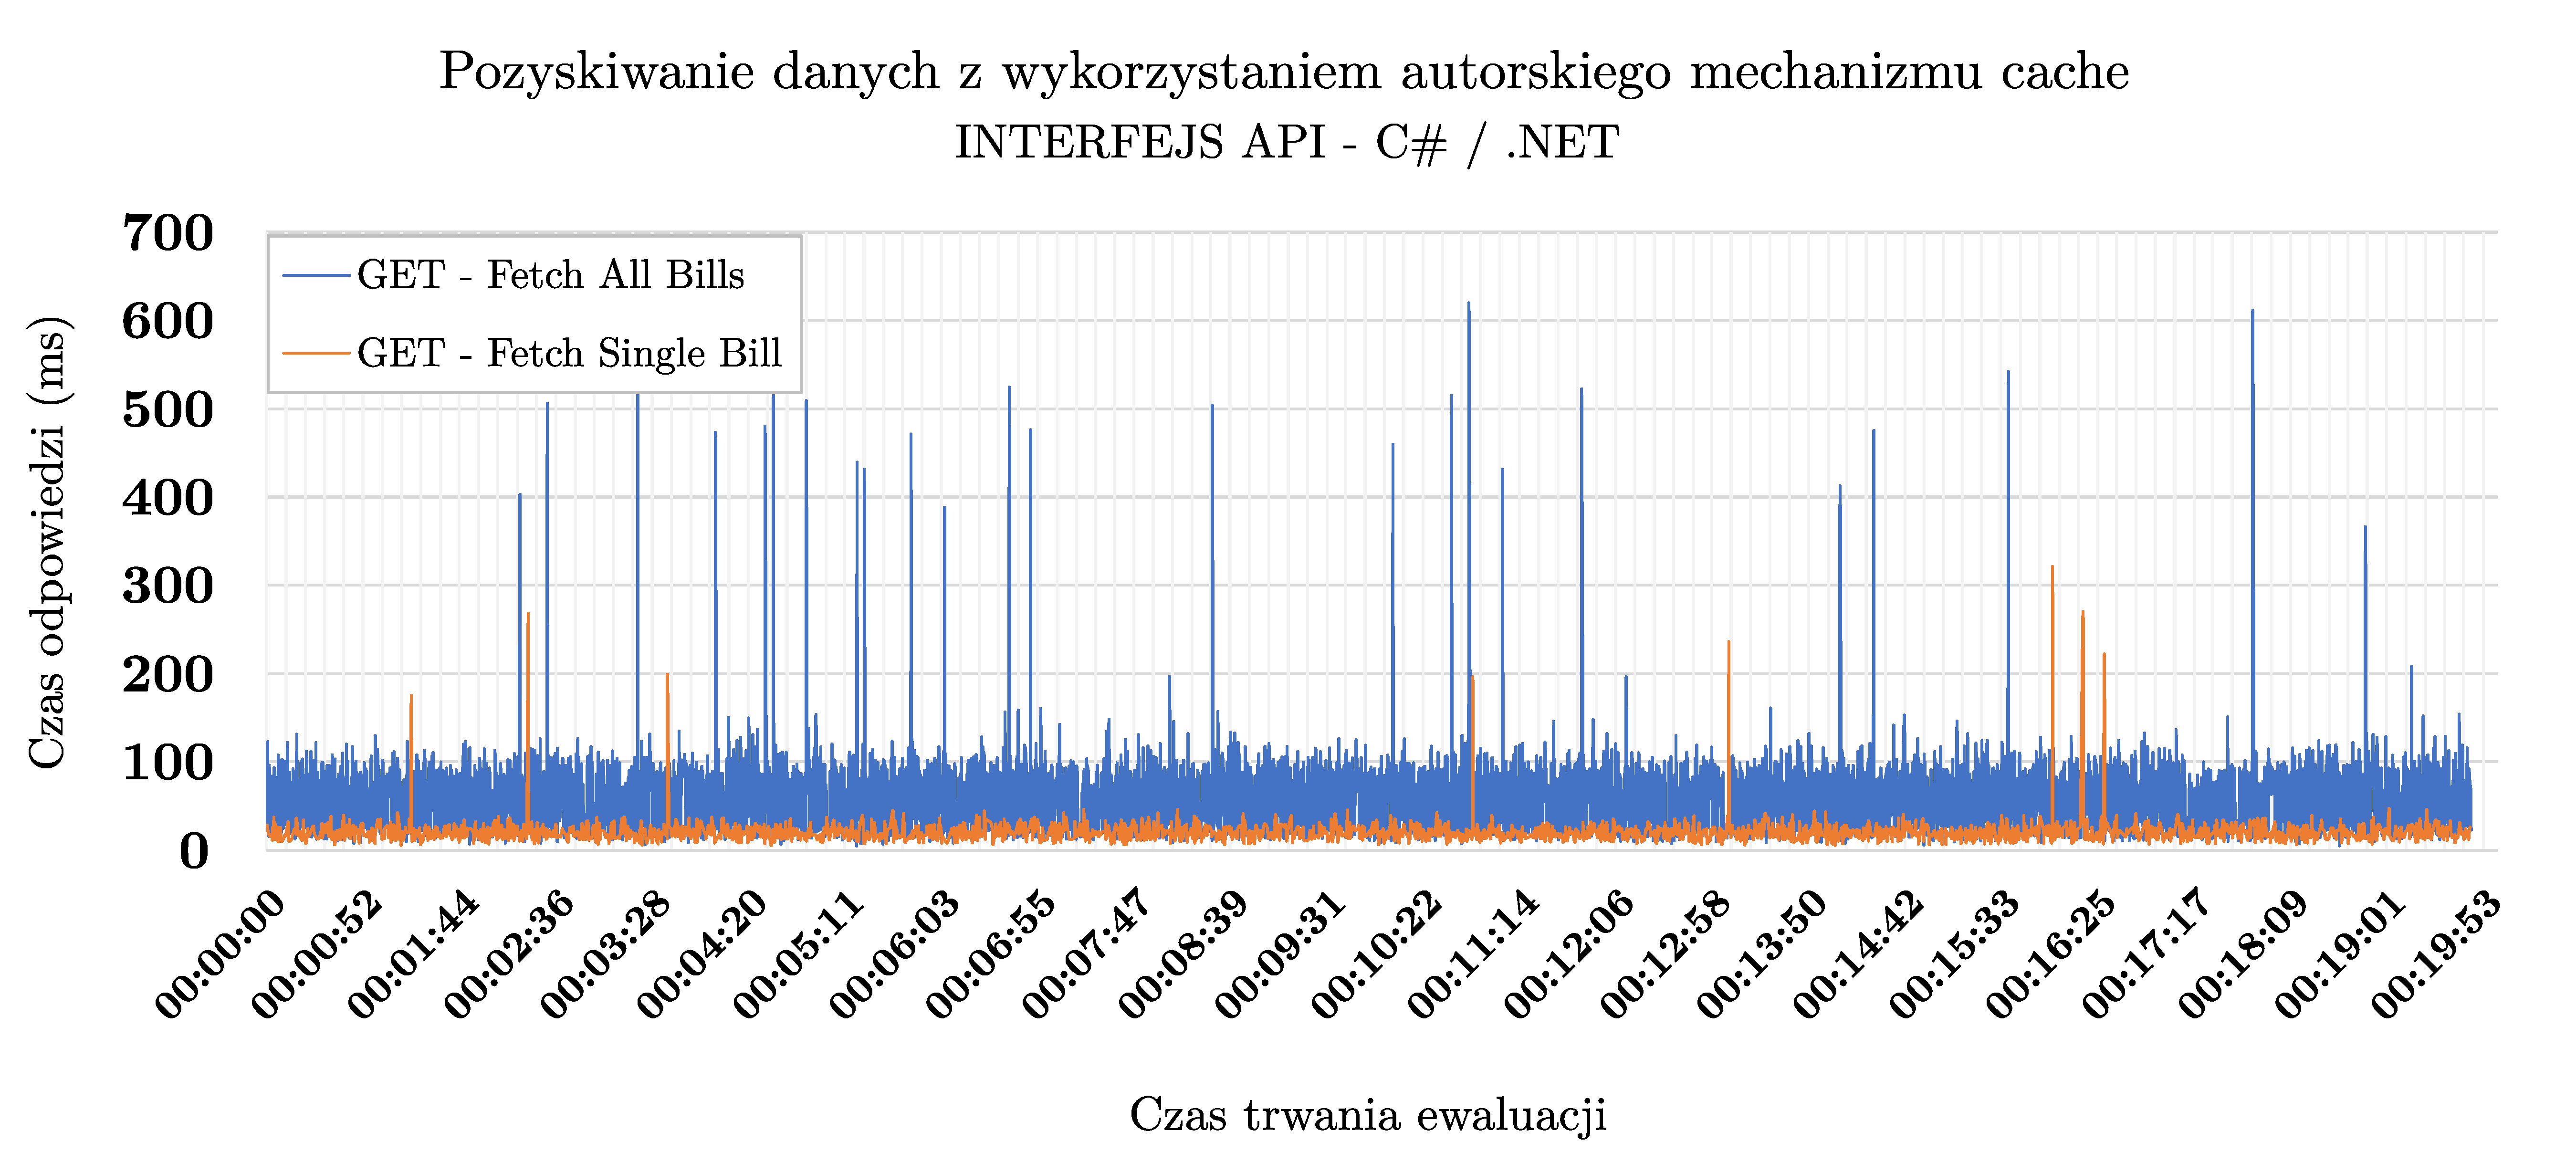
\includegraphics[width=0.49\textwidth]{rys05/dotnet-freq-cache-chart.pdf} \\
    c) & d) \\
    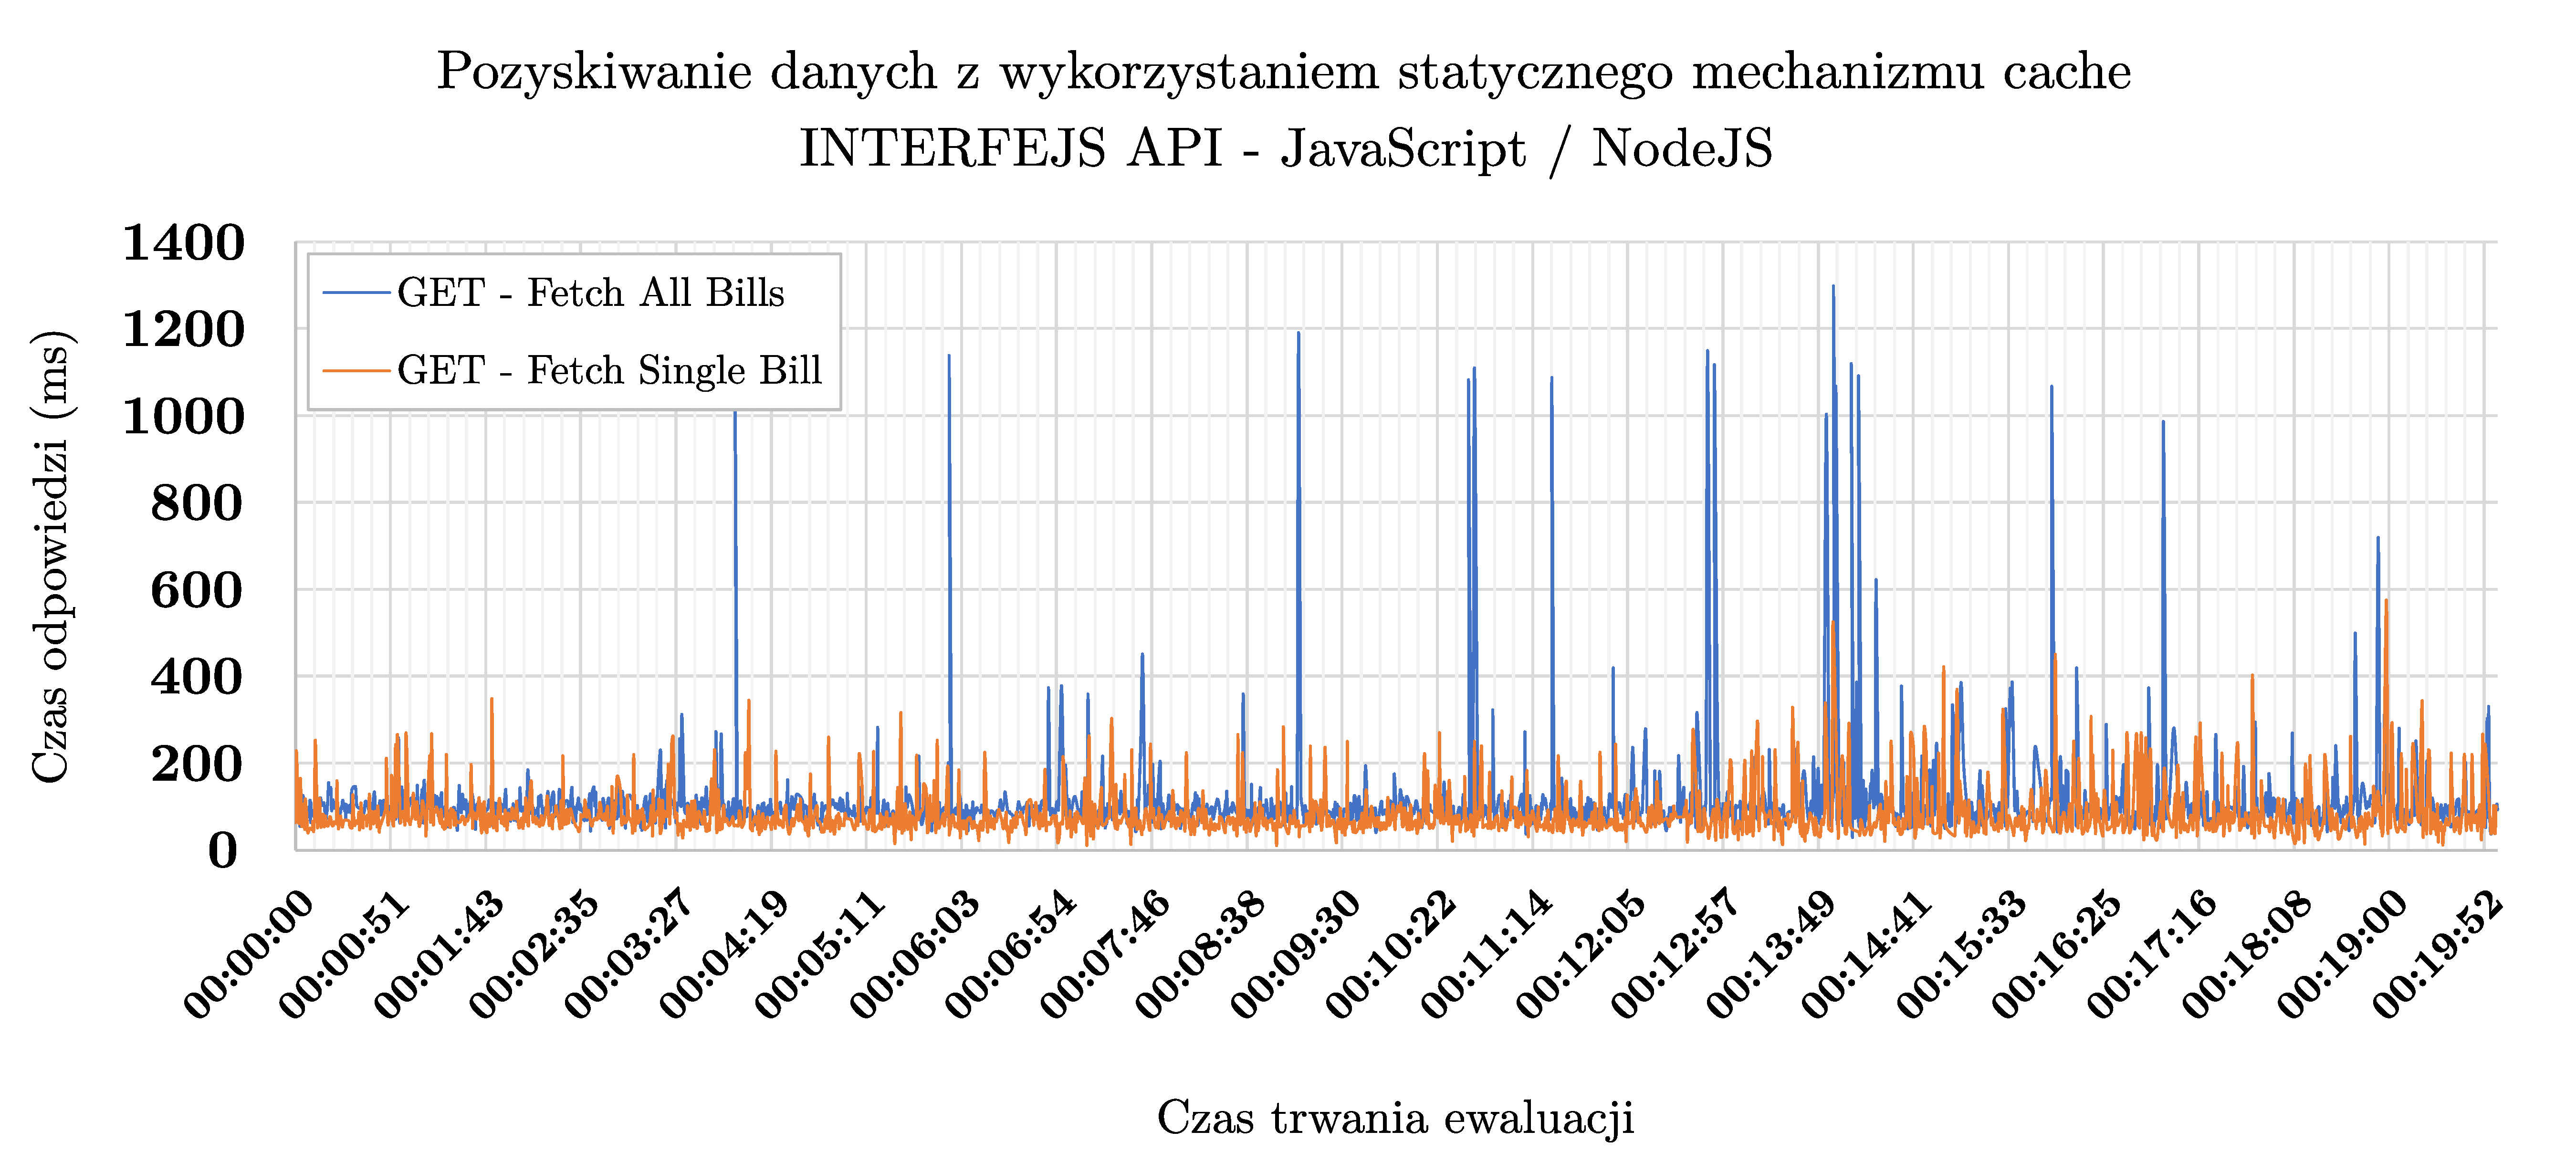
\includegraphics[width=0.49\textwidth]{rys05/nodejs-static-cache.pdf} & 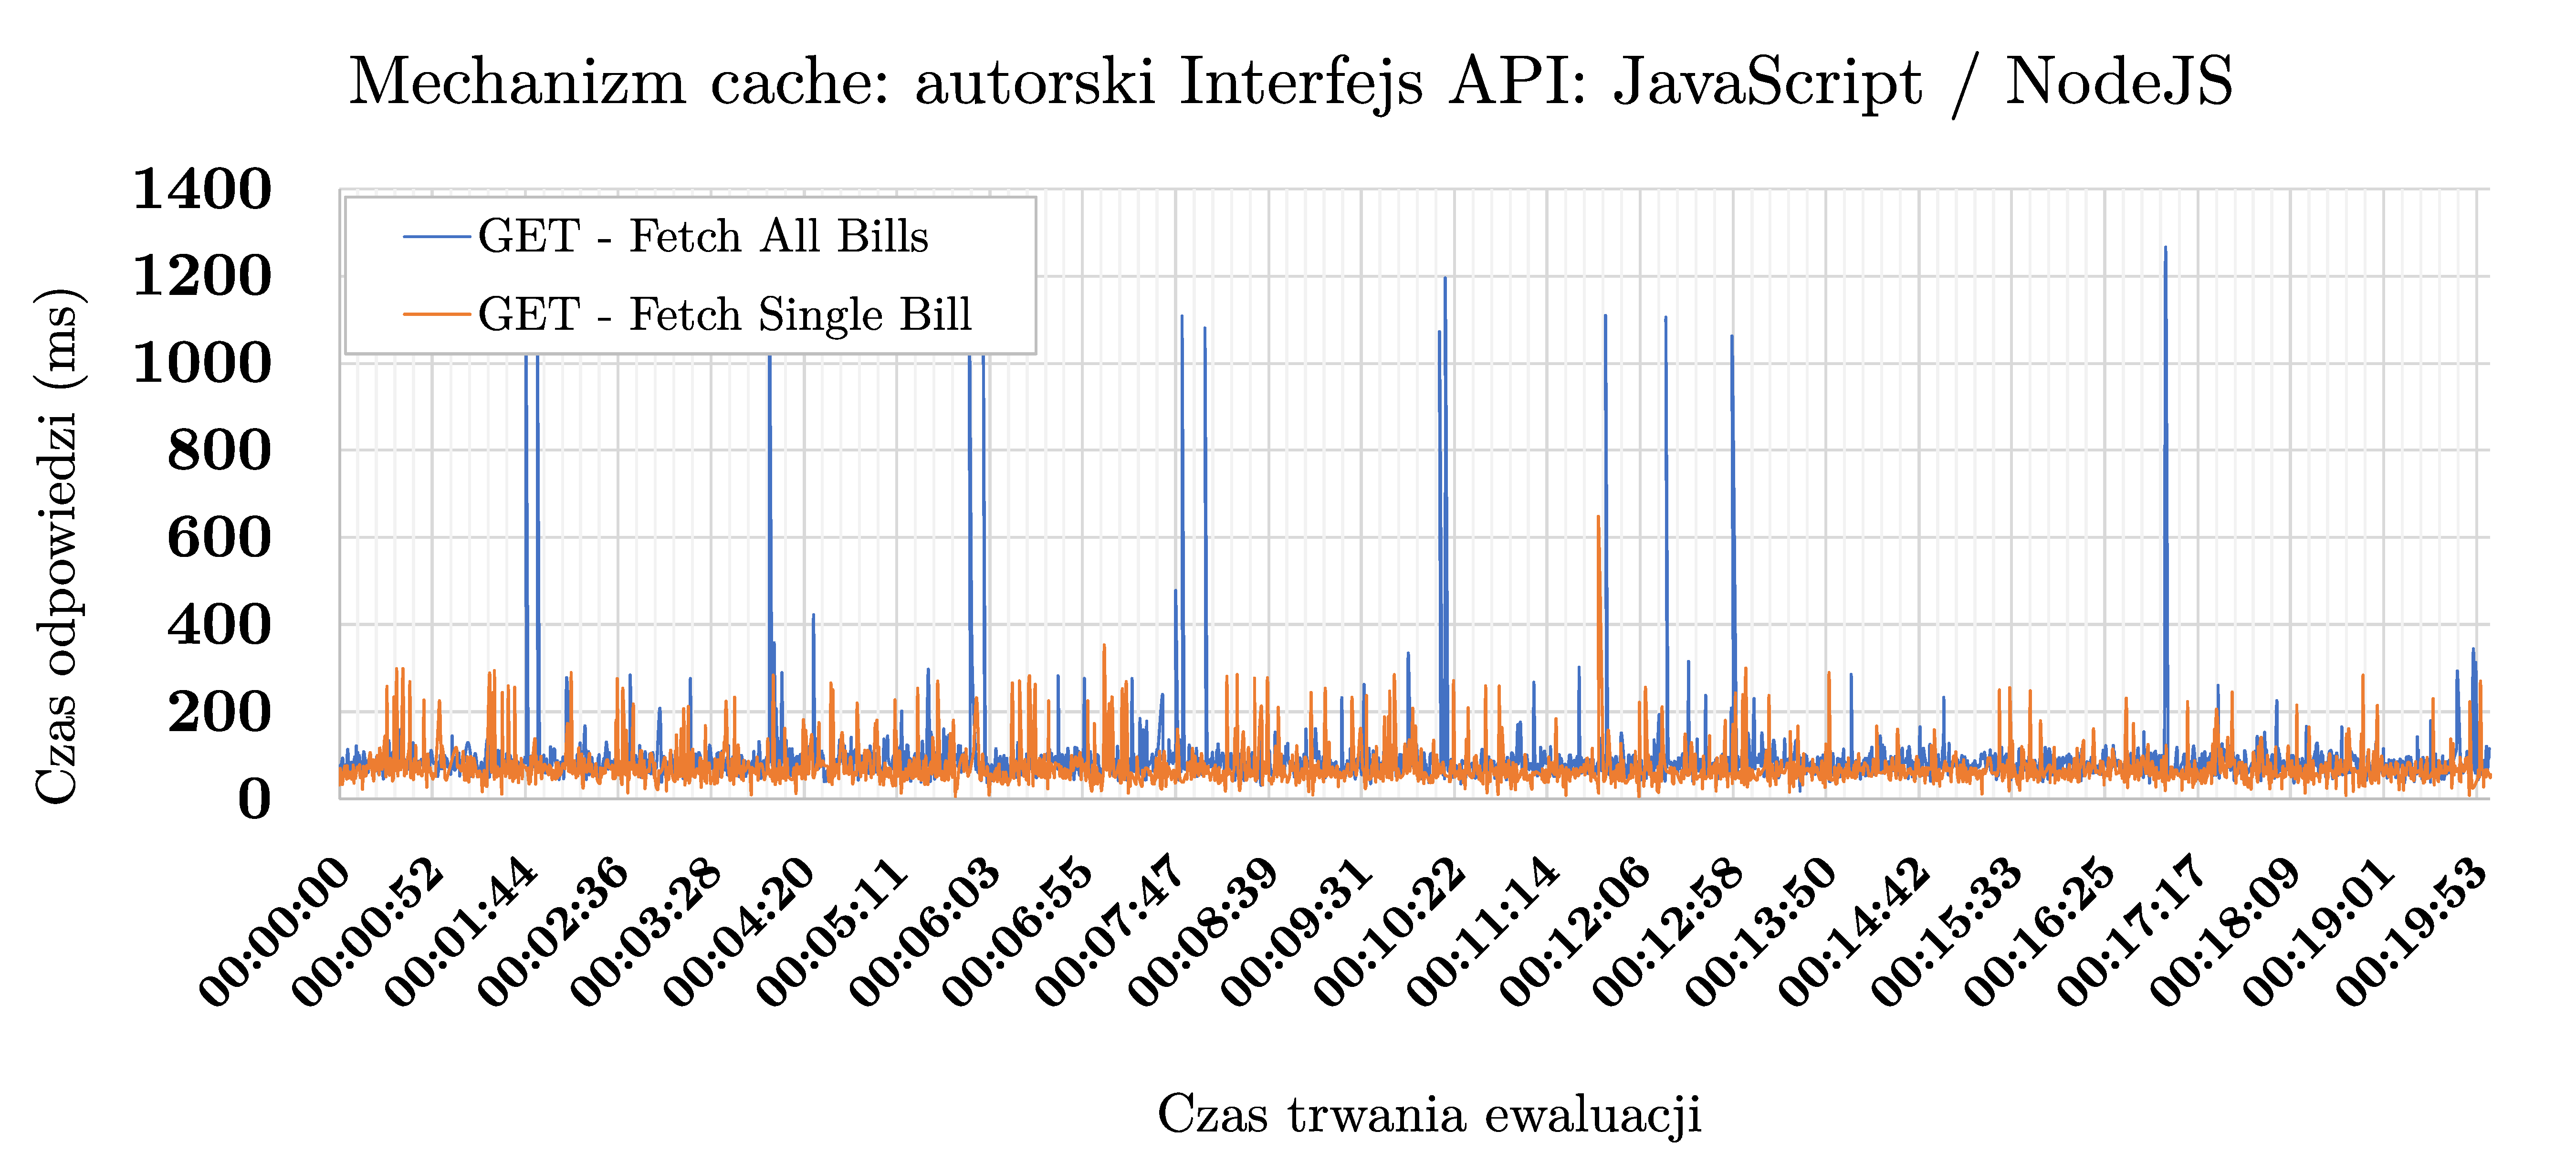
\includegraphics[width=0.49\textwidth]{rys05/nodejs-freq-cache.pdf}
    % jezeli obraki sa rownej wysokosci, mozna je wyrownac do gory stosujac vtop jak nizej
    % \vtop{\vskip-2ex\hbox{{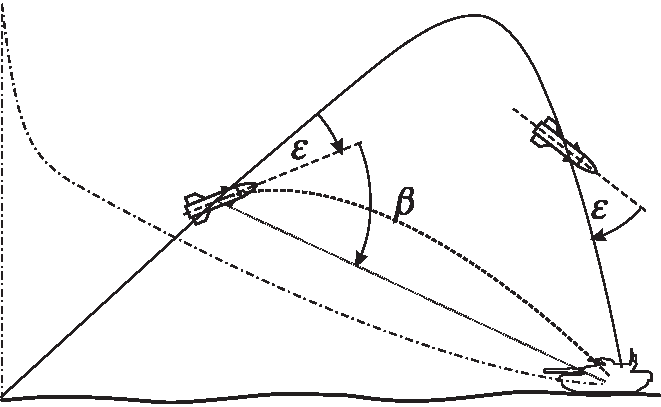
\includegraphics[width=0.475\textwidth]{rys05/beta1}}}} &
    % \vtop{\vskip-2ex\hbox{{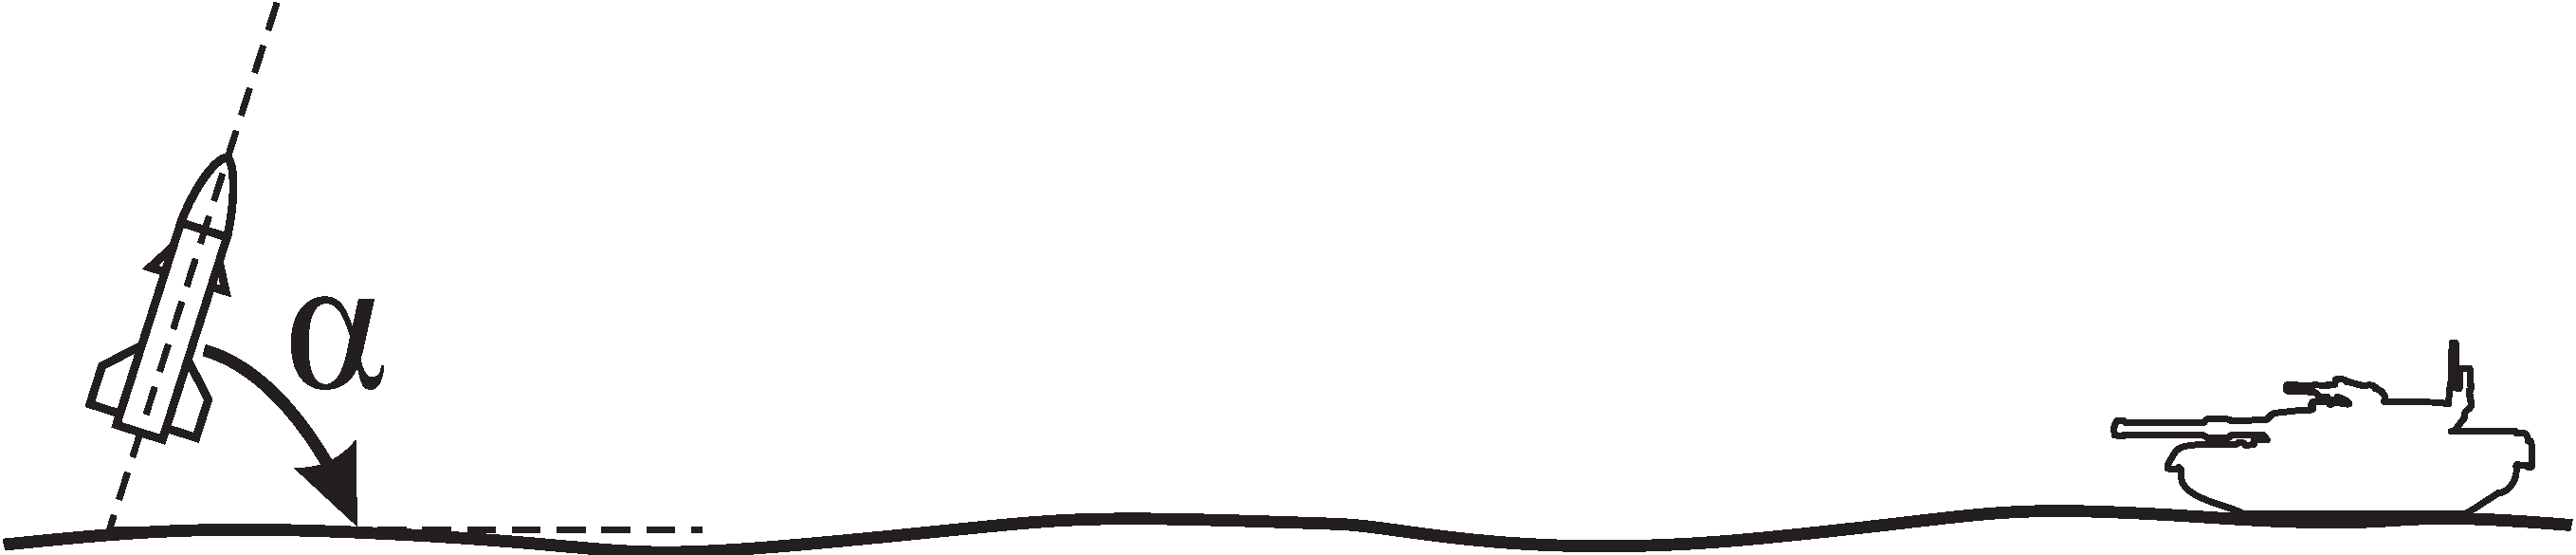
\includegraphics[width=0.475\textwidth]{rys05/alfa1}}}}  \caption{Wyznaczanie trajektorii lotu rakiety: 
    \end{tabular}
  \caption{Porównanie czasów odpowiedzi na żądanie dla odmiennych mechanizmów pamięci podręcznej}
  \label{fig:cache-charts}
\end{figure}

W kontekście interfejsu programowania aplikacji zaimplementowanego w języku C\# zauważyć możemy znaczące wydłużenie się przedziałów czasowych, w ramach których nie występują żądania o wysokim czasie odpowiedzi. Trend ten, nie jest jednakże tak dobrze dostrzegalny w odniesieniu eksperymentu przeprowadzanego z wykorzystaniem interfejsu API napisanego w JavaScript. Ponadto, niezależnie od technologii, nie jest zauważalne spodziewane, stopniowe rozszerzanie się odcinków niskich czasów odpowiedzi, wraz z postępem ewaluacji. Może to być spowodowane nieadekwatnymi wartościami liczników unieważnień, które określone zostały na podstawie poprzednich eksperymentów wykorzystujących mechanizm o stałym czasie przechowywania wpisu.
\section{Zmienność wydajności api wdrożonego na generycznej oraz dedykowanej platformie chmurowej}
Ostatnia ze zrealizowanych w ramach niniejszej pracy ewaluacji odnosi się do analizy zmiany wydajności pracy interfejsów programowania aplikacji w zależności od środowiska wdrożeniowego, w ramach którego usługa sieciowa jest hostowana. Celem niniejszego badania jest sprawdzenie, czy wykorzystanie dedykowanej rozwiązaniu platformy chmurowej, pozwala na uzyskanie lepszych rezultatów działania api, niż w przypadku wdrożenia systemu internetowego na infrastrukturze generycznej, którą jest wirtualny serwer prywatny.

Zdecydowano się na zastosowanie usługi w modelu infrastructure-as-a-service, która pełniła rolę środowiska produkcyjnego niezależnego od technologii implementacji api. W środowisku tym, wdrożono interfejsy programowania aplikacji napisane w językach C\# oraz JavaScript, wykorzystując serwer HTTP Apache oraz usługę odwróconego proxy. Ponadto, każda z poddawanych analizie usług, komunikowała się z silnikiem bazodanowym znajdującym się wewnątrz wirtualnego serwera prywatnego. Dzięki temu, wyeliminiować można było zjawisko zmienności czasu połączenia pomiędzy interfejsem a źródłem danych, która to zmienność wynika z niedeterministycznego charakteru łącza sieciowego. Aby zachować pełną generyczność omawianego rozwiązania zastosowano jeden z najpopularniejszych systemów bazodanowych jakim jest MySQL. System ten, choć w znaczącym stopniu wspierany przez aplikacje tworzone w językach C\# oraz JavaScript, nie jest rozwiązaniem postrzeganym jako dedykowane względem platform .NET oraz NodeJS. 

Jako podejścia referencyjne względem infrastruktury generycznej, wdrożone zostały interfejsy programowania aplikacji na platformach Microsoft Azure oraz Heroku. Pierwsza z nich, jest usługą dedykowaną dla rozwiązań bazujących na platformie .NET oraz napisanych w języku C\#. W tym przypadku, interfejs programowania aplikacji połączono z bazą danych Microsoft SQL Server. Druga z platform to rekomendowane rozwiązanie dla systemów internetowych tworzonych z wykorzystaniem środowiska uruchomieniowego NodeJS. Interfejs API wdrożony na platformie Heroku, skomunikowany został z nierelacyjną bazą danych MongoDB.

Odnosząc się do metryk gromadzonych w ramach niniejszego badania, wspomnieć należy o fakcie, że rezultaty wykonywanych operacji nie stanowią wartości czasu odpowiedzi na żądanie, a jedynie czas przetwarzania zapytania wewnątrz metody kontrolera interfejsu programowania aplikacji. Takie podejście, pozwala na uniezależnienie ewaluacji względem lokalizacji oraz szybkości łącza internetowego urządzeń generujących zapytania.

W przeprowadzonym badaniu generowano zapytania pod pięć punktów końcowych, które wykorzystywane były również w eksperymencie \ref{research:crud}. Ich szczegółowa charakterystyka zawarta została w tabeli \ref{tab:endpointy-scenario-1}. Przed rozpoczęciem analizy, zestawiono rozproszoną konfigurację topologii fizycznej nr 5, która opisana została w sekcji \ref{sec:rozproszone-srodowisko-badawcze-ver-1}, a także dokonano ewaluacji funkcjonalnej zaimplementowanych rozwiązań, poprzez realizację testów linii bazowej. Plan testowy obejmował uruchomienie 40 współbieżnie pracujących wątków oprogramowania Apache JMeter, które generowały ruch sieciowy przez 10 minut. Całość badania była przeprowadzona zgodnie ze zdefiniowanym uprzednio scenariuszem badawczym \ref{tab:research-scenario-6}.

Kluczowymi wskaźnikami wydajności rozwiązań wdrażanych na platformach chmurowych są: czas realizacji pojedynczego zapytania, procent błędnych odpowiedzi w kontekście poprawnych zapytań, a także efektywność wykorzystania zasobów fizycznego sprzętu. Zdecydowano się na pominięcie ostatniego z przytoczonych wskaźników, ponieważ w odniesieniu do tak przygotowanego badania, nie dostarcza on informacji, które mogłaby być przesłanką do formułowania jakichkolwiek hipotez dotyczących omawianego problemu. W czasie generowania zapytań w kierunku interfejsów programowania aplikacji, niezależnie od platform wdrożeniowych oraz uruchomieniowych, konsumpcja fizycznych zasobów sprzętowych cechowała się relatywną stałością w czasie. Oznacza to, że każda z poddawanych analizie platform chmurowych, jest w stanie obsłużyć znacząco większy ruch, niż ten, generowanych w ramach tego badania. Przeanalizowano natomiast, zarówno czas przetwarzania zapytania wewnątrz interfejsu, jak i liczbę błędnych zapytań w stosunku do wszystkich wygenerowanych.     

Na wykresach \ref{fig:dotnet-azure-vs-digitalocean} a) do \ref{fig:dotnet-azure-vs-digitalocean} h) zawarto porównanie rezultatów pozyskanych w czasie ewaluacji interfejsu programowania aplikacji napisanego w języku C\# i uruchamianego na platformach: generycznej (tj. DigitalOcean VPS), oraz dedykowanej (tj. Microsoft Azure).

\begin{figure}[htb]
  \centering
	\begin{tabular}{@{}ll@{}}
    a) & b) \\
    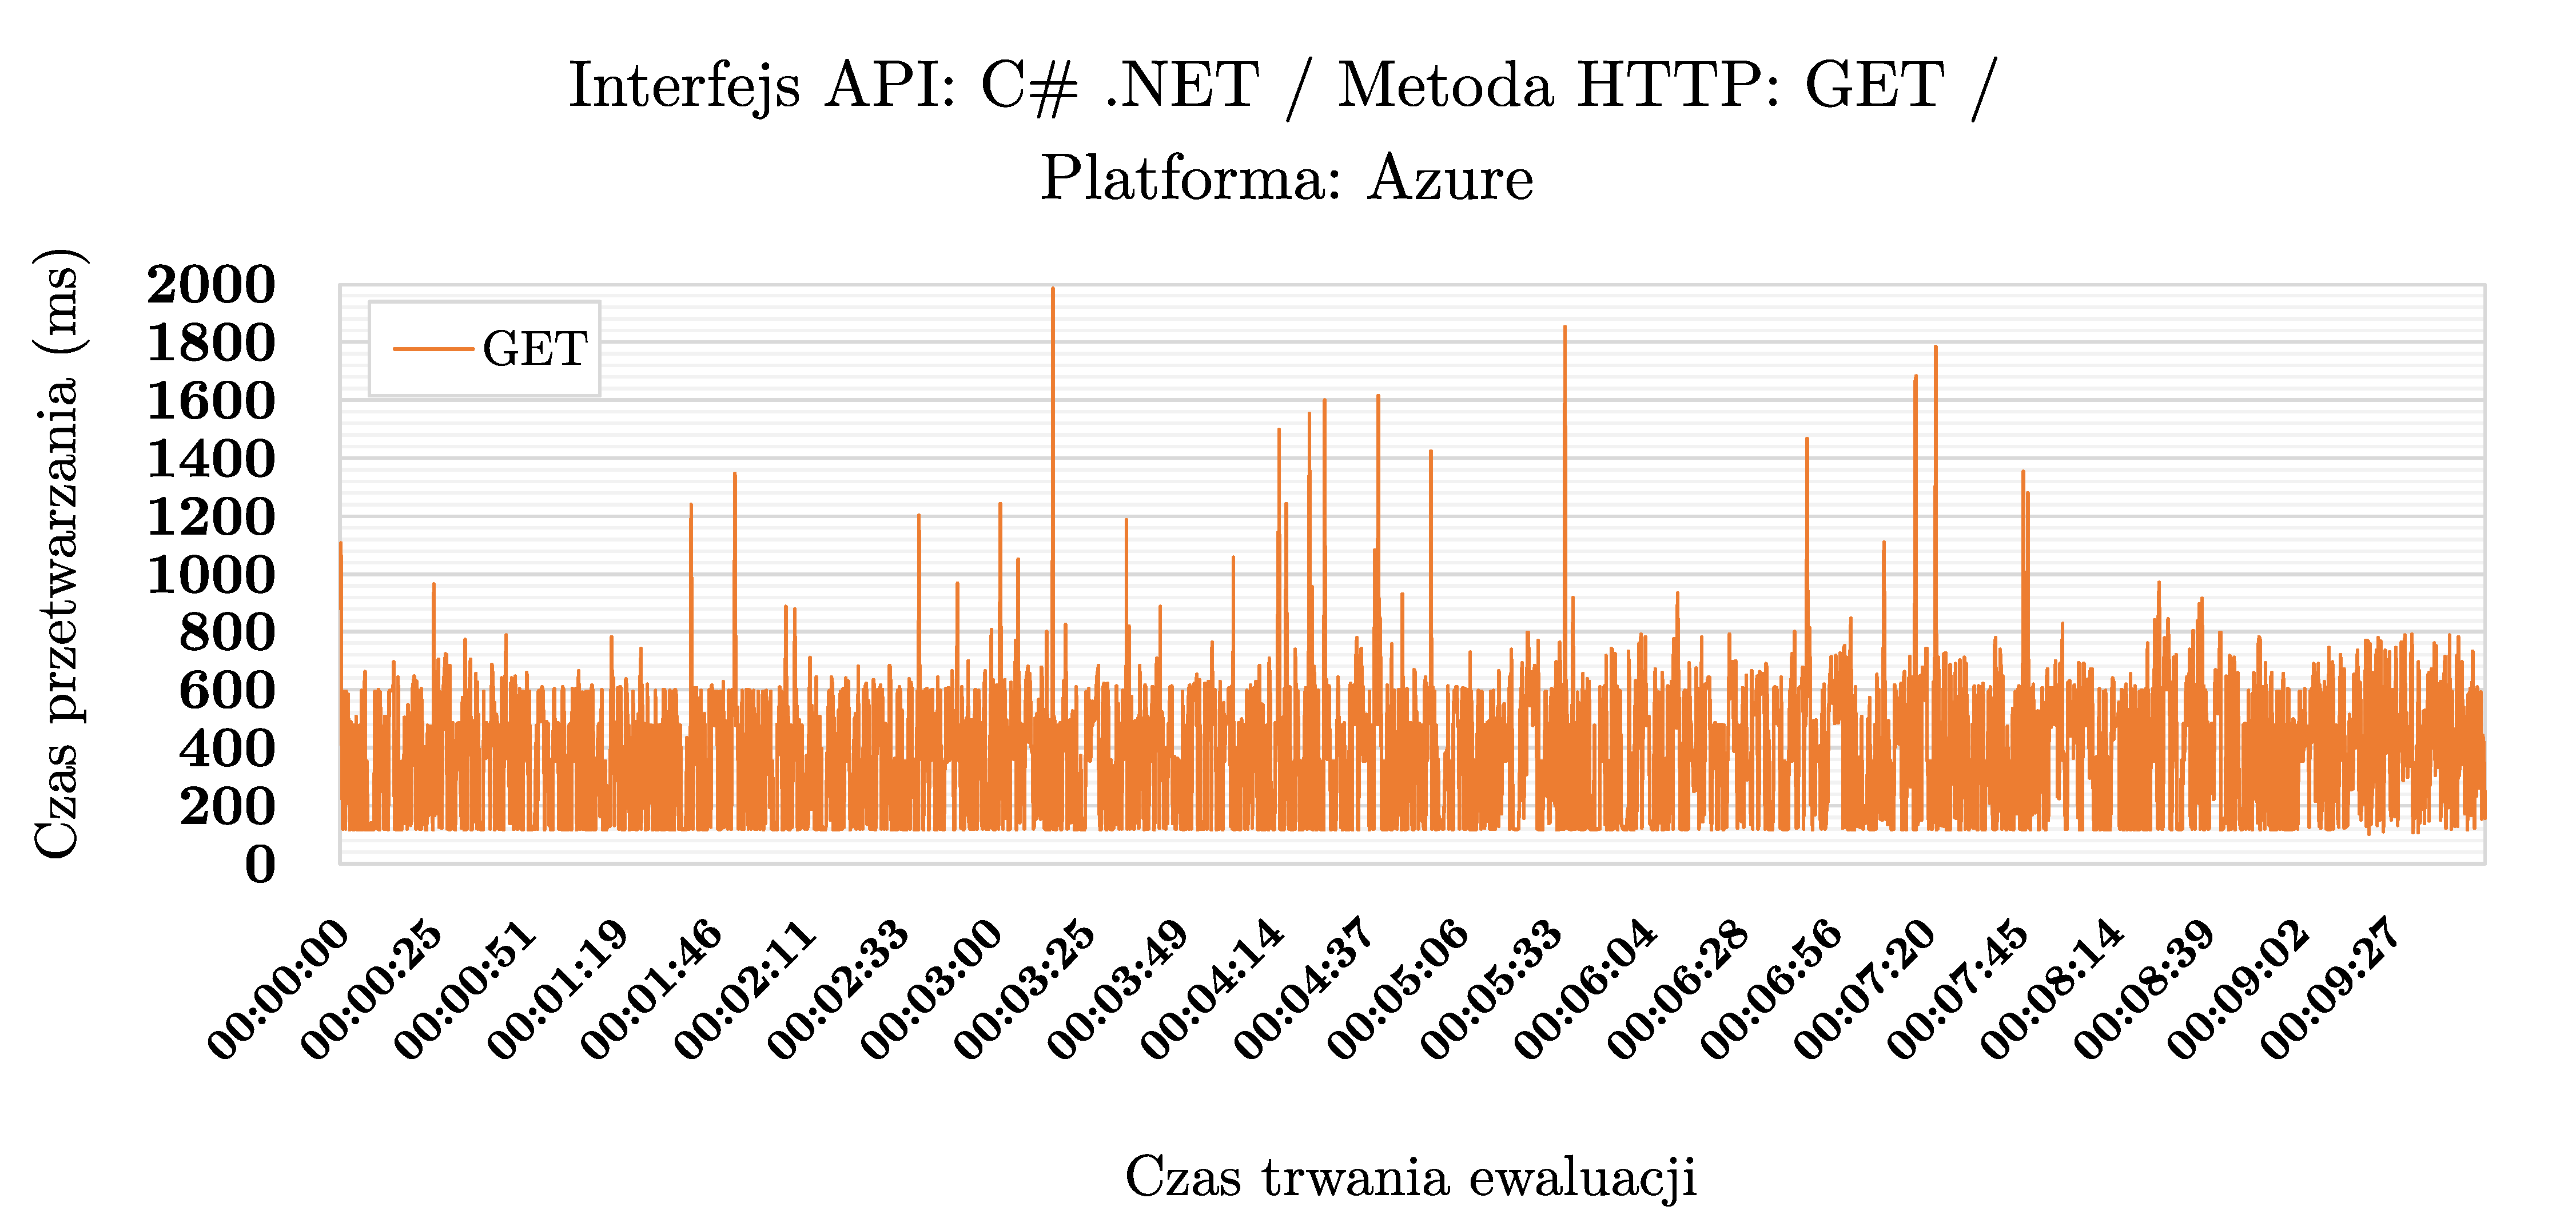
\includegraphics[width=0.49\textwidth]{rys05/dotnet-get-azure.pdf} & \includegraphics[width=0.49\textwidth]{rys05/dotnet-get-digitalocean.pdf} \\
    c) & d) \\
    \includegraphics[width=0.49\textwidth]{rys05/dotnet-post-azure.pdf} & \includegraphics[width=0.49\textwidth]{rys05/dotnet-post-digitalocean.pdf} \\
    e) & f) \\
    \includegraphics[width=0.49\textwidth]{rys05/dotnet-put-azure.pdf} & \includegraphics[width=0.49\textwidth]{rys05/dotnet-put-digitalocean.pdf} \\
    g) & h) \\
    \includegraphics[width=0.49\textwidth]{rys05/dotnet-delete-azure.pdf} & \includegraphics[width=0.49\textwidth]{rys05/dotnet-delete-digitalocean.pdf} \\
	% jezeli obraki sa rownej wysokosci, mozna je wyrownac do gory stosujac vtop jak nizej
	% \vtop{\vskip-2ex\hbox{{\includegraphics[width=0.475\textwidth]{rys05/beta1}}}} &
	% \vtop{\vskip-2ex\hbox{{\includegraphics[width=0.475\textwidth]{rys05/alfa1}}}}  \caption{Wyznaczanie trajektorii lotu rakiety: 
	\end{tabular}
  \caption{Wydajność działania mierzona czasem wewnętrznego przetwarzania operacji CRUD dla platform Azure oraz DigitalOcean -- Interfejs API C\# .NET}
  \label{fig:dotnet-azure-vs-digitalocean}
\end{figure}

Wskazać należy nieznaczą, jednakże występującą przewagę rozwiązania opartego o usługę platform-as-a-service. Jak możemy zauważyć, przewaga ta, występuje niezależnie od typu generowanego żądania klienta. Ponadto, w przypadku rozwiązania generycznego zaobserwowano pojawienie się większej liczby zapytań klienckich, których czasy odpowiedzi nie mieściły się w przedziale definiującym 97\% wszystkich próbek (tj. od 200 ms do 580 ms) dla rozwiązania dedykowanego. Szczególnie trend ten, widoczny jest dla żądań metody HTTP typu PUT. Wartym odnotowania jest fakt niewystępowania jakiegokolwiek wyniku w przedziale od 0 do 119 ms. Wyniki takie, były bez trudu osiągane w środowisku lokalnym dla małej liczby współbieżnie pracujących generatorów. Zjawisko to, jest specyficzne względem względem technologii C\# .NET i nie uwidacznia się w przypadku interfejsów uruchamianych w NodeJS.

\begin{figure}[H]
  \centering
	\begin{tabular}{@{}ll@{}}
    a) & b) \\
    \includegraphics[width=0.49\textwidth]{rys05/nodejs-get-heroku.pdf} & \includegraphics[width=0.49\textwidth]{rys05/nodejs-get-digitalocean.pdf} \\
    c) & d) \\
    \includegraphics[width=0.49\textwidth]{rys05/nodejs-post-heroku.pdf} & \includegraphics[width=0.49\textwidth]{rys05/nodejs-post-digitalocean.pdf} \\
    e) & f) \\
    \includegraphics[width=0.49\textwidth]{rys05/nodejs-put-heroku.pdf} & \includegraphics[width=0.49\textwidth]{rys05/nodejs-put-digitalocean.pdf} \\
    g) & h) \\
    \includegraphics[width=0.49\textwidth]{rys05/nodejs-delete-heroku.pdf} & \includegraphics[width=0.49\textwidth]{rys05/nodejs-delete-digitalocean.pdf} \\
	% jezeli obraki sa rownej wysokosci, mozna je wyrownac do gory stosujac vtop jak nizej
	% \vtop{\vskip-2ex\hbox{{\includegraphics[width=0.475\textwidth]{rys05/beta1}}}} &
	% \vtop{\vskip-2ex\hbox{{\includegraphics[width=0.475\textwidth]{rys05/alfa1}}}}  \caption{Wyznaczanie trajektorii lotu rakiety: 
	\end{tabular}
  \caption{Wydajność działania mierzona czasem wewnętrznego przetwarzania operacji CRUD dla platform Heroku oraz DigitalOcean -- Interfejs API NodeJS}
  \label{fig:nodejs-heroku-vs-digitalocean}
\end{figure}

Kolejna z zaprezentowanych wizualizacji, dotyczy z kolei interfejsu API zaimplementowanego w oparciu o technologię NodeJS, który uruchomiony został na platformie Heroku (konfiguracja dedykowana), a także serwerze udostępnianym w ramach chmury DigitalOcean (konfiguracja generyczna). Zgromadzone czasy przetwarzania żądań dla odmiennych typów operacji pokazane zostały na wykresach \ref{fig:nodejs-heroku-vs-digitalocean} a) do \ref{fig:nodejs-heroku-vs-digitalocean} h).

Odnosząc się do analizowanej technologii, wzrost wydajności rozwiązania dedykowanego względem generycznego jest wydatny, i niezależnie od wybranego typu wykonywanej operacji, różnica wartości metryki go opisującaj jest niemniejsza niż 237 ms. Ponadto, w momencie w którym 99,98\% wszystkich obserwacji należy do przedziału od 34 ms do 900 ms w kontekście rozwiązania dedykowanego, tylko 72,7\% próbek badania dla rozwiązania generycznego, zawarte jest w analogicznym przedziale. Zauważyć należy fakt braku zwiększenia się intensywności żądań dla czasów przetwarzania powyżej 1000 ms, w odniesieniu do rozwiązania generycznego. Co prawda zapytania trwające powyżej 1000 ms pojawiają się w tego typu konfiguracji, to podobnie do rozwiązania dedykowanego, są to obserwacje jednostkowe.  

Kolejną metryką wziętą pod uwagę w ramach niniejszego badania jest liczba niepoprawnych odpowiedzi, które zostały zwrócone dla wygenerowanych zapytań. Podobnie jak dla wizualizacji zaprezentowanych powyżej, w tym przypadku, analiza również prowadzona będzie pod kątem obserwacji różnic wynikających z zastosowania odmiennych platform wdrożeniowych, a nie technologii implementacji interfejsów api. Na wykresach \ref{fig:errors-for-plaforms} a) oraz \ref{fig:errors-for-plaforms} b) przedstawiono wartości odnotowane względem omawianej metryki.

\begin{figure}[htb]
  \centering
	\begin{tabular}{@{}ll@{}}
    a) & b) \\
    \includegraphics[width=0.49\textwidth]{rys05/nodejs-errors.pdf} & \includegraphics[width=0.49\textwidth]{rys05/dotnet-errors.pdf} \\
	% jezeli obraki sa rownej wysokosci, mozna je wyrownac do gory stosujac vtop jak nizej
	% \vtop{\vskip-2ex\hbox{{\includegraphics[width=0.475\textwidth]{rys05/beta1}}}} &
	% \vtop{\vskip-2ex\hbox{{\includegraphics[width=0.475\textwidth]{rys05/alfa1}}}}  \caption{Wyznaczanie trajektorii lotu rakiety: 
	\end{tabular}
  \caption{Liczba błędnych odpowiedzi względem typu żądania oraz platformy wdrożeniowej}
  \label{fig:errors-for-plaforms}
\end{figure}


W przypadku interfejsu implementowanego z wykorzystaniem platformy NodeJS oraz języka JavaScript różnice wydajnościowe uwidaczniają się jeszcze bardziej w momencie w którym brana pod uwagę jest liczba niepowodzeń realizacji zapytań klienckich. Niezależnie od typu operacji, rozwiązanie wdrożone na platformie Heroku, generowało mniejszą liczbę błędnych odpowiedzi. Przytaczając najbardziej skrajny przypadek (tj. żądania typu GET), liczba niezrealizowanych poprawnie zapytań dla platformy generycznej jest ponad dwa razy większa, od tej dla platformy dedykowanej.

Analogiczną tendencję zaobserwować możemy w przypadku interfejsu programowania aplikacji C\# .NET. Tu również, niezależnie od metody protokołu hipertekstowego, rozwiązanie rekomendowane przez twórcę technologii posiada przewagę. Przewaga ta, najbardziej widoczna jest dla żądania typu PUT i wynosi ona 37 niepoprawnych odpowiedzi. Warto zaznaczyć, że całkowita liczba błędnie zrealizowanych żądań dla metody PUT oraz platformy dedykowanej wynosi 26.

Wyniki przeprowadzonego w tej sekcji badania posiadają najbardziej jednoznaczny charakter spośród wszystkich rezultatów otrzymanych w kontekście każdego z przeprowadzonych badań. Co więcej, rezultaty te, prowadzą do sformułowania popartego badaniami wniosku, że niezależnie od faktu, która z technologii implementacyjnych zostanie wybrana, a także jakiego typu operacje będą realizowane, system internetowy przygotowany do przejścia w fazę produkcyjną, powinien być wdrażany z wykorzystaniem narzędzi oraz infrastruktur dedykowanych względem określonej technologii. Usprawnienia wydajnościowe, wprowadzane przez twórców określonych środowisk chmurowych, pozwalają na korzystanie z usług sieciowych w sposób bardziej efektywny, a także generujący mniejszą liczbę błędów.
\chapter{Podsumowanie}
\section{Uzyskane efekty pracy}
Celem niniejszej pracy była ewaluacja wydajności interfejsów programowania aplikacji implementowanych w dwóch różnych technologiach, w odniesieniu do licznych aspektów dotyczących sposobów ich wykorzystania. Zdecydowano się, nie tylko na analizę efektywności podstawowych rodzajów operacji protokołu hipertekstowego, wchodzących w skład tak popularnych dzisiaj usług sieciowych, ale także wykorzystania mechanizmów programowania współbieżnego, technik obsługi żądań asynchronicznych, implementacji zaawansowanego wzorca projektowego, zastosowania rozwiniętych technik optymalizacji pozyskiwania danych, a także wdrożenia rozwiązań w kontekście środowisk chmurowych.

Zwrócenie uwagi na tak wiele aspektów dotyczących interfejsów programowania aplikacji miało na celu uświadomienie czytelnika, że tego typu systemy internetowe, wykorzystywane są powszechnie nie tylko do realizacji najpopularniejszych czterech, podstawowych operacji na danych. Wachlarz możliwości związanych z tworzeniem internetowych API jest znacząco szerszy, a fakt ten uwydatnia się wraz z rosnącym poziomem skomplikowania usług sieciowych, a także zadań, które są przed nimi stawiane.

Zastosowanie mnogości kontekstów, w których odnaleźć musiały się były przygotowane rozwiązania, miało też odmienny cel. Misją autora było dowiedzenie się czy którykolwiek z systemów opartych o dwie porównywane technologie wdrożeniowo-uruchomieniowe, wykazuje wysoką wydajność względem swojego konkurenta w którymkolwiek z obszarów prowadzonych badań. Jeżeli tak, to które z tych obszarów są faworyzowane przez konkretne technologie.

Wyniki przeprowadzonych badań umożliwiły rozwianie powyższych wątpliwości, a także uzyskanie dodatkowej wiedzy, która nawet dla osób posiadających doświadczenie w zakresie kompozycji oraz tworzenia interfejsów API, nie musi wydawać się oczywista. Zrealizowane eksperymenty uwidoczniły niektóre zależności, zadając innym z kolei kłam. Przykładem potwierdzenia spodziewanej hipotezy, może być wykazana wyższość wydajności rozwiązań implementowanych na platformach dedykowanych względem platform generycznych. Kolejną egzemplifikacją, w ramach której, jeszcze przed przeprowadzeniem badania, sformułować można było silną hipotezę, była obserwacja wpływu zastosowania usprawnień wydajnościowych, separacji środowisk bazodanowych, a także wdrożenia wzorca podziału odpowiedzialności. Rezultaty badania systemów bazodanowych z kolei, mogą być doskonałym argumentem, na obalenie hipotezy wyższej efektywności komunikacji silników baz danych oraz interfejsów tworzonych na bazie technologii jednego producenta.

Odnosząc się do dodatkowej wiedzy, której chęć pozyskiwania wzmożona została poprzez ambicję wyjaśnienia pojawiających się w badaniach anomalii, wspomnieć należy o sposobie obsługi wielowątkowej w odniesieniu do współbieżnie generowanych, długotrwających żądań. Obsługa ta, niemalże nie występuje w kontekście interfejsu języka JavaScript, natomiast jest wydatnie rozbudowana w przypadku usługi implementowanej w C\# i uruchamianej na platformie .NET. Ponadto, ciekawym jest również fakt, jak bardzo prostota, tycząca się mechanizmów wywoływania operacji asynchronicznych, może nieść korzyść dotyczącą wydajności ich realizacji.

W niektórych przypadkach jednak, konwencjonalność rozwiązania nie idzie w parze z jego wydajnością. Potwierdzeniem tego właśnie stwierdzenia są przeprowadzone badania dotyczące podstawowego oraz autorskiego podejścia do realizacji mechanizmów pamięci podręcznej. W ramach pracy tej, zaimplementowano, a także zbadano zachowanie systemu cache uwzględniającego częstotliwość wywoływania punktu końcowego, a także liczbę unieważnień identyfikującego go wpisu. Zgromadzone rezultaty należy postrzegać jako obiecujące, jednakże wymagana jest zdecydowanie bardzej obszerna analiza uwzględniająca zmienność liczby momentów unieważnień, czy też wpływ dysproporcji parametrów w różnych chwilach obsługi żądań.

Wspomnieć należy również o przeprowadzonych w ramach niniejszego badania parowych testach statystycznych, które pozwoliły na wykazanie statystycznie istotnej przewagi określonych konfiguracji rozwiązań względem pozostałych z nich. 

Bardzo ważnym jest również uwypuklenie pewnej tezy. Przeprowadzony zestaw badań nie wskazał, jednakże przede wszystkim nie miał wskazać, technologii niezaprzeczalnie lepszej. Technologia taka nie istnieje, a wynika to w głównej mierze z ilości obszarów, w kontekście których może ona zostać wykorzystana oraz badana. Dlatego też, dokument ten, może okazać się pomocny dla tych osób, którzy zainteresowani są oceną poziomu wydajności interfejsu dla konkretnej technologii oraz konkretnego sposobu jej wykorzystania.
\section{Perspektywy rozwoju badań}
Każdy z przytoczonych obszarów wykorzystania interfejsów programowania aplikacji, reprezentowany w niniejszej pracy poprzez odmienne badanie, może zostać z łatwością rozbudowany poprzez ewaluację dodatkowych metryk wydajnościowych, czy też zmianę konfiguracji środowiska badawczego. Zdecydowano się na wskazanie perspektyw rozwoju badań w odniesieniu do tych domen funkcjonalności API, które zostały poruszone w tym dokumencie.

Odwołując się do badania wpływu wykorzystania systemów bazodanowych w kontekście porównywanych technologii, jako perspektywę rozwoju wskazać należy przeprowadzenie ewaluacji wydajności dla przedziałów liczby wątków-generatorów o zmiennej długości. Ponadto, wzięte pod uwagę mogą być również te spośród systemów bazodanowych, w ramach których nie dostarczane jest wsparcie dla mapperów obiektowo-relacyjnych Entity Framework Core oraz Prisma.

W ramach badania realizacji operacji współbieżnych, wprowadzić można dodatkowe rodzaje algorytmów metaheurystycznych dla różnych problemów o wysokiej złożoności obliczeniowej. Interesującą perspektywą rozwoju tego badania, jest również implementacja odmiennych heurystyk dla symetrycznego problemu komiwojażera, a także porównanie ich wykonania dla interfejsów wspierających przetwarzanie wielowątkowe.

Badanie wydajności operacji asynchronicznych może zostać poszerzone o uwzględnienie różnych implementacji klientów protokołu hipertekstowego, a także konfiguracji poszczególnych ich parametrów.

Najwięcej perspektyw rozwoju badań, wyróżnić należy w kontekście ewaluacji porównywanych mechanizmów pamięci podręcznej. Zbadane mogą zostać między innymi odmienne metryki wpływające na zmianę czasu odpowiedzi na żądanie. Jako przykładową metrykę wskazać można narzut wydajnościowy wprowadzany przez metodę kalkulacji czasu życia wpisu w magazynie pamięci podręcznej. Ponadto, struktura wykonanego badania, mogłaby zostać dostosowana względem zmiennego czasu trwania testu, zmiennego natężenia ruchu sieciowego, czy też deterministycznego charakteru wywoływania żądań unieważniających. Co więcej, zaproponowana przez autora metoda może zostać zmodyfikowana poprzez uzależnienie czasu przechowywania wpisu od dodatkowych parametrów, bądź też zmianę ich istotności względem wyliczania czasu życia elementu pamięci cache.

W kontekście wprowadzenia wzorca podziału odpowiedzialności, a także separacji modeli bazodanowych, badanie może zostać poszerzone o zastosowanie odmiennych mechanizmów replikacji, niż wykorzystana w tej pracy technika transakcyjna. W takim przypadku, należy zbadać w jakim czasie, od momentu dodania rekordu bazodanowego, będzie on dostępny w ramach źródła danych przeznaczonego do odczytu. Co więcej, należy pamiętać, że celem zdefiniowania specyficznej struktury obsługi żądania, była możliwość optymalizacji modeli danych. Dlatego też, interesującą perspektywą rozwoju tego badania, mogłoby być wskazanie, które z zaimplementowanych technik optymalizacji mają kluczowe znaczenie pod kątem wydajności, a które wpływają na nią jedynie nieznacznie.

Ostatnie ze zidentyfikowanych perspektyw rozwoju tyczą się obserwacji efektywności działania w odniesieniu do produkcyjnych środowisk chmurowych. Biorąc pod uwagę ten właśnie aspekt, możliwym jest dokonanie porównania dla większej liczby platform wdrożeniowych, czy też zbadanie, w jaki sposób usługi generyczne typu infrastructure-as-a-service mogą zostać zoptymalizowane, aby implementowane wewnątrz nich systemy internetowe, osiągały wydajność przybliżoną, lub wyższą względem rozwiązań dedykowanych. 


%\bibliographystyle{plalpha}
\bibliographystyle{plabbrv}

%UWAGA: bibliotek referencji naley przygotowa samemu. Dobrym do tego narzdziem jest JabRef.
%       Nazw przygotowanej biblioteki wpisuje si poniej bez rozszerzenia 
%       (w tym przypadku jest to "dokumentacja.bib")
\setlength{\bibitemsep}{2pt} % - by zacieni wykaz literatury
%\addtocontents{toc}{\addvspace{5pt}} % ustawiamy odstp przed literatur w spisie treci
\bibliography{dokumentacja}
\appendix
\chapter{Instrukcja instalacji}
Zasady przyznawania stopnia naukowego doktora i doktora habilitowanego w Polsce określa ustawa z dnia 14 marca 2003 r. o stopniach naukowych i~tytule naukowym oraz o stopniach i~tytule w zakresie sztuki (Dz.U. nr 65 z 2003 r., poz. 595 (Dz. U. z 2003 r. Nr 65, poz. 595). Poprzednie polskie uregulowania nie wymagały bezwzględnie posiadania przez kandydata tytułu zawodowego magistra lub równorzędnego (choć zasada ta zazwyczaj była przestrzegana) i zdarzały się nadzwyczajne przypadki nadawania stopnia naukowego doktora osobom bez studiów wyższych, np. słynnemu matematykowi lwowskiemu – późniejszemu profesorowi Stefanowi Banachowi. 

W innych krajach również zazwyczaj do przyznania stopnia naukowego doktora potrzebny jest dyplom ukończenia uczelni wyższej, ale nie wszędzie.


\chapter{Opis załączonej płyty CD/DVD}
Tutaj jest miejsce na zamieszczenie opisu zawartości załączonej płyty.
Należy wymienić, co zawiera.

% Ponisze jest niepotrzebne, jeli nie generuje si indeksu
%%\chapterstyle{noNumbered}
%%\phantomsection % sets an anchor
%%\addcontentsline{toc}{chapter}{Indeks rzeczowy}
%%\printindex

\end{document}
